% Options for packages loaded elsewhere
\PassOptionsToPackage{unicode}{hyperref}
\PassOptionsToPackage{hyphens}{url}
\PassOptionsToPackage{dvipsnames,svgnames,x11names}{xcolor}
%
\documentclass[
  a4paper,
]{scrreport}

\usepackage{amsmath,amssymb}
\usepackage{iftex}
\ifPDFTeX
  \usepackage[T1]{fontenc}
  \usepackage[utf8]{inputenc}
  \usepackage{textcomp} % provide euro and other symbols
\else % if luatex or xetex
  \usepackage{unicode-math}
  \defaultfontfeatures{Scale=MatchLowercase}
  \defaultfontfeatures[\rmfamily]{Ligatures=TeX,Scale=1}
\fi
\usepackage{lmodern}
\ifPDFTeX\else  
    % xetex/luatex font selection
\fi
% Use upquote if available, for straight quotes in verbatim environments
\IfFileExists{upquote.sty}{\usepackage{upquote}}{}
\IfFileExists{microtype.sty}{% use microtype if available
  \usepackage[]{microtype}
  \UseMicrotypeSet[protrusion]{basicmath} % disable protrusion for tt fonts
}{}
\makeatletter
\@ifundefined{KOMAClassName}{% if non-KOMA class
  \IfFileExists{parskip.sty}{%
    \usepackage{parskip}
  }{% else
    \setlength{\parindent}{0pt}
    \setlength{\parskip}{6pt plus 2pt minus 1pt}}
}{% if KOMA class
  \KOMAoptions{parskip=half}}
\makeatother
\usepackage{xcolor}
\setlength{\emergencystretch}{3em} % prevent overfull lines
\setcounter{secnumdepth}{5}
% Make \paragraph and \subparagraph free-standing
\ifx\paragraph\undefined\else
  \let\oldparagraph\paragraph
  \renewcommand{\paragraph}[1]{\oldparagraph{#1}\mbox{}}
\fi
\ifx\subparagraph\undefined\else
  \let\oldsubparagraph\subparagraph
  \renewcommand{\subparagraph}[1]{\oldsubparagraph{#1}\mbox{}}
\fi

\usepackage{color}
\usepackage{fancyvrb}
\newcommand{\VerbBar}{|}
\newcommand{\VERB}{\Verb[commandchars=\\\{\}]}
\DefineVerbatimEnvironment{Highlighting}{Verbatim}{commandchars=\\\{\}}
% Add ',fontsize=\small' for more characters per line
\usepackage{framed}
\definecolor{shadecolor}{RGB}{241,243,245}
\newenvironment{Shaded}{\begin{snugshade}}{\end{snugshade}}
\newcommand{\AlertTok}[1]{\textcolor[rgb]{0.68,0.00,0.00}{#1}}
\newcommand{\AnnotationTok}[1]{\textcolor[rgb]{0.37,0.37,0.37}{#1}}
\newcommand{\AttributeTok}[1]{\textcolor[rgb]{0.40,0.45,0.13}{#1}}
\newcommand{\BaseNTok}[1]{\textcolor[rgb]{0.68,0.00,0.00}{#1}}
\newcommand{\BuiltInTok}[1]{\textcolor[rgb]{0.00,0.23,0.31}{#1}}
\newcommand{\CharTok}[1]{\textcolor[rgb]{0.13,0.47,0.30}{#1}}
\newcommand{\CommentTok}[1]{\textcolor[rgb]{0.37,0.37,0.37}{#1}}
\newcommand{\CommentVarTok}[1]{\textcolor[rgb]{0.37,0.37,0.37}{\textit{#1}}}
\newcommand{\ConstantTok}[1]{\textcolor[rgb]{0.56,0.35,0.01}{#1}}
\newcommand{\ControlFlowTok}[1]{\textcolor[rgb]{0.00,0.23,0.31}{#1}}
\newcommand{\DataTypeTok}[1]{\textcolor[rgb]{0.68,0.00,0.00}{#1}}
\newcommand{\DecValTok}[1]{\textcolor[rgb]{0.68,0.00,0.00}{#1}}
\newcommand{\DocumentationTok}[1]{\textcolor[rgb]{0.37,0.37,0.37}{\textit{#1}}}
\newcommand{\ErrorTok}[1]{\textcolor[rgb]{0.68,0.00,0.00}{#1}}
\newcommand{\ExtensionTok}[1]{\textcolor[rgb]{0.00,0.23,0.31}{#1}}
\newcommand{\FloatTok}[1]{\textcolor[rgb]{0.68,0.00,0.00}{#1}}
\newcommand{\FunctionTok}[1]{\textcolor[rgb]{0.28,0.35,0.67}{#1}}
\newcommand{\ImportTok}[1]{\textcolor[rgb]{0.00,0.46,0.62}{#1}}
\newcommand{\InformationTok}[1]{\textcolor[rgb]{0.37,0.37,0.37}{#1}}
\newcommand{\KeywordTok}[1]{\textcolor[rgb]{0.00,0.23,0.31}{#1}}
\newcommand{\NormalTok}[1]{\textcolor[rgb]{0.00,0.23,0.31}{#1}}
\newcommand{\OperatorTok}[1]{\textcolor[rgb]{0.37,0.37,0.37}{#1}}
\newcommand{\OtherTok}[1]{\textcolor[rgb]{0.00,0.23,0.31}{#1}}
\newcommand{\PreprocessorTok}[1]{\textcolor[rgb]{0.68,0.00,0.00}{#1}}
\newcommand{\RegionMarkerTok}[1]{\textcolor[rgb]{0.00,0.23,0.31}{#1}}
\newcommand{\SpecialCharTok}[1]{\textcolor[rgb]{0.37,0.37,0.37}{#1}}
\newcommand{\SpecialStringTok}[1]{\textcolor[rgb]{0.13,0.47,0.30}{#1}}
\newcommand{\StringTok}[1]{\textcolor[rgb]{0.13,0.47,0.30}{#1}}
\newcommand{\VariableTok}[1]{\textcolor[rgb]{0.07,0.07,0.07}{#1}}
\newcommand{\VerbatimStringTok}[1]{\textcolor[rgb]{0.13,0.47,0.30}{#1}}
\newcommand{\WarningTok}[1]{\textcolor[rgb]{0.37,0.37,0.37}{\textit{#1}}}

\providecommand{\tightlist}{%
  \setlength{\itemsep}{0pt}\setlength{\parskip}{0pt}}\usepackage{longtable,booktabs,array}
\usepackage{calc} % for calculating minipage widths
% Correct order of tables after \paragraph or \subparagraph
\usepackage{etoolbox}
\makeatletter
\patchcmd\longtable{\par}{\if@noskipsec\mbox{}\fi\par}{}{}
\makeatother
% Allow footnotes in longtable head/foot
\IfFileExists{footnotehyper.sty}{\usepackage{footnotehyper}}{\usepackage{footnote}}
\makesavenoteenv{longtable}
\usepackage{graphicx}
\makeatletter
\def\maxwidth{\ifdim\Gin@nat@width>\linewidth\linewidth\else\Gin@nat@width\fi}
\def\maxheight{\ifdim\Gin@nat@height>\textheight\textheight\else\Gin@nat@height\fi}
\makeatother
% Scale images if necessary, so that they will not overflow the page
% margins by default, and it is still possible to overwrite the defaults
% using explicit options in \includegraphics[width, height, ...]{}
\setkeys{Gin}{width=\maxwidth,height=\maxheight,keepaspectratio}
% Set default figure placement to htbp
\makeatletter
\def\fps@figure{htbp}
\makeatother

\usepackage{venndiagram}
\newcommand{\NN}{\mathbb{N}}
\newcommand{\ZZ}{\mathbb{Z}}
\newcommand{\QQ}{\mathbb{Q}}
\newcommand{\RR}{\mathbb{R}}
\newcommand{\CC}{\mathbb{C}}
\DeclareMathOperator{\operatorname{Int}}{Int}
\DeclareMathOperator{\operatorname{Ext}}{Ext}
\DeclareMathOperator{\operatorname{Fr}}{Fr}
\DeclareMathOperator{\Adh}{Adh}
\DeclareMathOperator{\Ac}{Ac}
\DeclareMathOperator{\sen}{sen}
\makeatletter
\@ifpackageloaded{tcolorbox}{}{\usepackage[skins,breakable]{tcolorbox}}
\@ifpackageloaded{fontawesome5}{}{\usepackage{fontawesome5}}
\definecolor{quarto-callout-color}{HTML}{909090}
\definecolor{quarto-callout-note-color}{HTML}{0758E5}
\definecolor{quarto-callout-important-color}{HTML}{CC1914}
\definecolor{quarto-callout-warning-color}{HTML}{EB9113}
\definecolor{quarto-callout-tip-color}{HTML}{00A047}
\definecolor{quarto-callout-caution-color}{HTML}{FC5300}
\definecolor{quarto-callout-color-frame}{HTML}{acacac}
\definecolor{quarto-callout-note-color-frame}{HTML}{4582ec}
\definecolor{quarto-callout-important-color-frame}{HTML}{d9534f}
\definecolor{quarto-callout-warning-color-frame}{HTML}{f0ad4e}
\definecolor{quarto-callout-tip-color-frame}{HTML}{02b875}
\definecolor{quarto-callout-caution-color-frame}{HTML}{fd7e14}
\makeatother
\makeatletter
\@ifpackageloaded{bookmark}{}{\usepackage{bookmark}}
\makeatother
\makeatletter
\@ifpackageloaded{caption}{}{\usepackage{caption}}
\AtBeginDocument{%
\ifdefined\contentsname
  \renewcommand*\contentsname{Tabla de contenidos}
\else
  \newcommand\contentsname{Tabla de contenidos}
\fi
\ifdefined\listfigurename
  \renewcommand*\listfigurename{Listado de Figuras}
\else
  \newcommand\listfigurename{Listado de Figuras}
\fi
\ifdefined\listtablename
  \renewcommand*\listtablename{Listado de Tablas}
\else
  \newcommand\listtablename{Listado de Tablas}
\fi
\ifdefined\figurename
  \renewcommand*\figurename{Figura}
\else
  \newcommand\figurename{Figura}
\fi
\ifdefined\tablename
  \renewcommand*\tablename{Tabla}
\else
  \newcommand\tablename{Tabla}
\fi
}
\@ifpackageloaded{float}{}{\usepackage{float}}
\floatstyle{ruled}
\@ifundefined{c@chapter}{\newfloat{codelisting}{h}{lop}}{\newfloat{codelisting}{h}{lop}[chapter]}
\floatname{codelisting}{Listado}
\newcommand*\listoflistings{\listof{codelisting}{Listado de Listados}}
\usepackage{amsthm}
\theoremstyle{definition}
\newtheorem{exercise}{Ejercicio}[chapter]
\theoremstyle{remark}
\AtBeginDocument{\renewcommand*{\proofname}{Prueba}}
\newtheorem*{remark}{Observación}
\newtheorem*{solution}{Solución}
\newtheorem{refremark}{Observación}[chapter]
\newtheorem{refsolution}{Solución}[chapter]
\makeatother
\makeatletter
\makeatother
\makeatletter
\@ifpackageloaded{caption}{}{\usepackage{caption}}
\@ifpackageloaded{subcaption}{}{\usepackage{subcaption}}
\makeatother
\ifLuaTeX
\usepackage[bidi=basic]{babel}
\else
\usepackage[bidi=default]{babel}
\fi
\babelprovide[main,import]{spanish}
% get rid of language-specific shorthands (see #6817):
\let\LanguageShortHands\languageshorthands
\def\languageshorthands#1{}
\ifLuaTeX
  \usepackage{selnolig}  % disable illegal ligatures
\fi
\usepackage{bookmark}

\IfFileExists{xurl.sty}{\usepackage{xurl}}{} % add URL line breaks if available
\urlstyle{same} % disable monospaced font for URLs
\hypersetup{
  pdftitle={Prácticas de Estadística con R},
  pdfauthor={Alfredo Sánchez Alberca},
  pdflang={es},
  colorlinks=true,
  linkcolor={blue},
  filecolor={Maroon},
  citecolor={Blue},
  urlcolor={Blue},
  pdfcreator={LaTeX via pandoc}}

\title{Prácticas de Estadística con R}
\author{Alfredo Sánchez Alberca}
\date{2022-01-06}

\begin{document}
\begin{titlepage}

%\AddToShipoutPicture*{\put(0,0){\includegraphics[scale=0.8]{img/background2}}} % Imagen de fondo, requiere el paquete eso-pic.
\begin{center}
\vspace*{5cm}

\Huge
{\textbf{\textsf{Prácticas de Estadística con R}}}

\vspace{0.5cm}
\LARGE
{\textbf{\textsf{}}}

\vspace{1.5cm}


\includegraphics[width=0.4\textwidth]{img/logos/sticker-estadistica-r.png}
\end{center}

\vfill

\begin{flushleft}
\begin{tabular}{ll}

\includegraphics[width=0.1\textwidth]{img/logos/aprendeconalf.png} & \parbox[b]{5cm}{\Large\textsf{Alfredo
Sánchez
Alberca}\\ \textsf{asalber@ceu.es} \\ \textsf{https://aprendeconalf.es}}
\end{tabular}
\end{flushleft}
\end{titlepage}
\renewcommand*\contentsname{Tabla de contenidos}
{
\hypersetup{linkcolor=}
\setcounter{tocdepth}{2}
\tableofcontents
}
\bookmarksetup{startatroot}

\chapter*{Prefacio}\label{prefacio}
\addcontentsline{toc}{chapter}{Prefacio}

\markboth{Prefacio}{Prefacio}

¡Bienvenido a Prácticas de Estadística con R!

Este libro presenta una recopilación de prácticas de Estadística
Descriptiva e Inferencial con el lenguaje de programación
\href{https://www.r-project.org/}{R}, con problemas aplicados a las
Ciencias y las Ingenierías.

No es un libro para aprender a programar con R, ya que solo enseña el
uso del lenguaje y de algunos de sus paquetes para resolver problemas de
Estadística. Para quienes estén interesados en aprender a programar en
este lenguaje, os recomiendo leer este
\href{https://aprendeconalf.es/manual-r/}{manual de R}.

\section*{Capítulos}\label{capuxedtulos}
\addcontentsline{toc}{section}{Capítulos}

\markright{Capítulos}

\phantomsection\label{toc}

\section*{Licencia}\label{licencia}
\addcontentsline{toc}{section}{Licencia}

\markright{Licencia}

Esta obra está bajo una licencia Reconocimiento -- No comercial --
Compartir bajo la misma licencia 3.0 España de Creative Commons. Para
ver una copia de esta licencia, visite
\url{https://creativecommons.org/licenses/by-nc-sa/3.0/es/}.

Con esta licencia eres libre de:

\begin{itemize}
\tightlist
\item
  Copiar, distribuir y mostrar este trabajo.
\item
  Realizar modificaciones de este trabajo.
\end{itemize}

Bajo las siguientes condiciones:

\begin{itemize}
\item
  \textbf{Reconocimiento}. Debe reconocer los créditos de la obra de la
  manera especificada por el autor o el licenciador (pero no de una
  manera que sugiera que tiene su apoyo o apoyan el uso que hace de su
  obra).
\item
  \textbf{No comercial}. No puede utilizar esta obra para fines
  comerciales.
\item
  \textbf{Compartir bajo la misma licencia}. Si altera o transforma esta
  obra, o genera una obra derivada, sólo puede distribuir la obra
  generada bajo una licencia idéntica a ésta.
\end{itemize}

Al reutilizar o distribuir la obra, tiene que dejar bien claro los
términos de la licencia de esta obra.

Estas condiciones pueden no aplicarse si se obtiene el permiso del
titular de los derechos de autor.

Nada en esta licencia menoscaba o restringe los derechos morales del
autor.

\bookmarksetup{startatroot}

\chapter{Introducción a R}\label{introducciuxf3n-a-r}

La gran potencia de cómputo alcanzada por los ordenadores ha convertido
a los mismos en poderosas herramientas al servicio de todas aquellas
disciplinas que, como la Estadística, requieren manejar un gran volumen
de datos. Actualmente, prácticamente nadie se plantea hacer un estudio
estadístico serio sin la ayuda de un buen programa de análisis de datos.

\emph{R} es un potente lenguaje de programación que incluye multitud de
funciones para la representación y el análisis de datos. Fue
desarrollado por Robert Gentleman y Ross Ihaka en la Universidad de
Auckland en Nueva Zelanda, aunque actualmente es mantenido por una
enorme comunidad científica en todo el mundo.

\begin{figure}[H]

{\centering 
\includegraphics[width=0.25\textwidth,height=\textheight]{img/logos/Rlogo.png}

}

\caption{Logotipo de R}

\end{figure}%

Las ventajas de R frente a otros programas habituales de análisis de
datos, como pueden ser SPSS, SAS o Matlab, son múltiples:

\begin{itemize}
\tightlist
\item
  Es software libre y por tanto gratuito. Puede descargarse desde la web
  \url{http://www.r-project.org/}.
\item
  Es multiplataforma. Existen versiones para Windows, Macintosh, Linux y
  otras plataformas.
\item
  Está avalado y en constante desarrollo por una amplia comunidad
  científica distribuida por todo el mundo que lo utiliza como estándar
  para el análisis de datos.
\item
  Cuenta con multitud de paquetes para todo tipo de análisis
  estadísticos y representaciones gráficas, desde los más habituales,
  hasta los más novedosos y sofisticados que no incluyen otros
  programas. Los paquetes están organizados y documentados en un
  \href{https://cran.r-project.org/}{repositorio CRAN} (Comprehensive R
  Archive Network) desde donde pueden descargarse libremente.
\item
  Es programable, lo que permite que el usuario pueda crear fácilmente
  sus propias funciones o paquetes para análisis de datos específicos.
  Existen multitud de libros, manuales y tutoriales libres que permiten
  su aprendizaje e ilustran el análisis estadístico de datos en
  distintas disciplinas científicas como las Matemáticas, la Física, la
  Biología, la Psicología, la Medicina, etc.
\end{itemize}

\section{Instalación de R}\label{instalaciuxf3n-de-r}

R puede descargarse desde el \href{https://www.r-project.org/}{sitio web
oficial de R} o desde el repositorio principal de paquetes de R
\href{https://cran.r-project.org/}{CRAN}. Basta con descargar el archivo
de instalación correspondiente al sistema operativo de nuestro ordenador
y realizar la instalación como cualquier otro programa.

El intérprete de R se arranca desde la terminal, aunque en Windows
incorpora su propia aplicación, pero es muy básica. En general, para
trabajos serios, conviene utilizar un entorno de desarrollo para R.

\section{Entornos de desarrollo}\label{entornos-de-desarrollo}

Por defecto el entorno de trabajo de R es en línea de comandos, lo que
significa que los cálculos y los análisis se realizan mediante comandos
o instrucciones que el usuario teclea en una ventana de texto. No
obstante, existen distintas interfaces gráficas de usuario que facilitan
su uso, sobre todo para usuarios noveles. Algunas de ellas, como las que
se enumeran a continuación, son completos entornos de desarrollo que
facilitan la gestión de cualquier proyecto:

\begin{itemize}
\item
  \href{https://www.rstudio.com/}{RStudio}. Probablemente el entorno de
  desarrollo más extendido para programar con R ya que incorpora
  multitud de utilidades para facilitar la programación con R.
\item
  \href{https://rkward.kde.org}{RKWard}. Es otra otro de los entornos de
  desarrollo más completos que además incluye a posibilidad de añadir
  nuevos menús y cuadros de diálogo personalizados.
\item
  \href{https://code.visualstudio.com/}{Visual Studio Code}. Es un
  entorno de desarrollo de propósito general ampliamente extendido.
  Aunque no es un entorno de desarrollo específico para R, incluye una
  extensión con utilidades que facilitan mucho el desarrollo con R.
\end{itemize}

\bookmarksetup{startatroot}

\chapter{Preprocesamiento de datos}\label{preprocesamiento-de-datos}

\section{Ejercicios Resueltos}\label{ejercicios-resueltos}

Para la realización de esta práctica se requieren los paquetes
\texttt{readr} y
\href{https://aprendeconalf.es/manual-r/06-preprocesamiento.html\#el-paquete-dplyr}{\texttt{dplyr}}
de la colección de paquetes
\href{https://aprendeconalf.es/manual-r/06-preprocesamiento.html\#la-colecci\%C3\%B3n-de-paquetes-tidyverse}{\texttt{tidyverse}}.

\begin{Shaded}
\begin{Highlighting}[]
\FunctionTok{library}\NormalTok{(tidyverse) }
\CommentTok{\# Incluye los siguientes paquetes:}
\CommentTok{\# {-} readr: para la lectura de ficheros csv. }
\CommentTok{\# {-} dplyr: para el preprocesamiento y manipulación de datos.}
\end{Highlighting}
\end{Shaded}

\begin{exercise}[]\protect\hypertarget{exr-preprocesamiento-1}{}\label{exr-preprocesamiento-1}

La siguiente tabla contiene los ingresos y gastos de una empresa durante
el primer trimestre del año.

\begin{tabu} to \linewidth {>{\raggedright}X>{\raggedleft}X>{\raggedleft}X>{\raggedleft}X}
\hline
Mes & Ingresos & Gastos & Impuestos\\
\hline
Enero & 45000 & 33400 & 6450\\
\hline
Febrero & 41500 & 35400 & 6300\\
\hline
Marzo & 51200 & 35600 & 7100\\
\hline
\end{tabu}

\begin{enumerate}
\def\labelenumi{\alph{enumi}.}
\item
  Crear un data frame con los datos de la tabla.

  \begin{tcolorbox}[enhanced jigsaw, toprule=.15mm, rightrule=.15mm, arc=.35mm, colback=white, colbacktitle=quarto-callout-tip-color!10!white, toptitle=1mm, left=2mm, colframe=quarto-callout-tip-color-frame, opacityback=0, breakable, opacitybacktitle=0.6, bottomtitle=1mm, titlerule=0mm, title=\textcolor{quarto-callout-tip-color}{\faLightbulb}\hspace{0.5em}{Solución}, bottomrule=.15mm, coltitle=black, leftrule=.75mm]

\begin{Shaded}
\begin{Highlighting}[]
\NormalTok{df }\OtherTok{\textless{}{-}} \FunctionTok{data.frame}\NormalTok{(}
    \AttributeTok{Mes =} \FunctionTok{c}\NormalTok{(}\StringTok{"Enero"}\NormalTok{, }\StringTok{"Febrero"}\NormalTok{, }\StringTok{"Marzo"}\NormalTok{),}
    \AttributeTok{Ingresos =} \FunctionTok{c}\NormalTok{(}\DecValTok{45000}\NormalTok{, }\DecValTok{41500}\NormalTok{, }\DecValTok{51200}\NormalTok{),}
    \AttributeTok{Gastos =} \FunctionTok{c}\NormalTok{(}\DecValTok{33400}\NormalTok{, }\DecValTok{35400}\NormalTok{, }\DecValTok{35600}\NormalTok{)}
\NormalTok{    )}
\NormalTok{df }
\end{Highlighting}
\end{Shaded}

\begin{verbatim}
      Mes Ingresos Gastos
1   Enero    45000  33400
2 Febrero    41500  35400
3   Marzo    51200  35600
\end{verbatim}

  \end{tcolorbox}
\item
  Añadir una nueva columna con los siguientes impuestos pagados.

  \begin{table}
  \centering
  \begin{tabular}{l|r}
  \hline
  Mes & Impuestos\\
  \hline
  Enero & 6450\\
  \hline
  Febrero & 6300\\
  \hline
  Marzo & 7100\\
  \hline
  \end{tabular}
  \end{table}

  \begin{tcolorbox}[enhanced jigsaw, toprule=.15mm, rightrule=.15mm, arc=.35mm, colback=white, colbacktitle=quarto-callout-tip-color!10!white, toptitle=1mm, left=2mm, colframe=quarto-callout-tip-color-frame, opacityback=0, breakable, opacitybacktitle=0.6, bottomtitle=1mm, titlerule=0mm, title=\textcolor{quarto-callout-tip-color}{\faLightbulb}\hspace{0.5em}{Solución 1}, bottomrule=.15mm, coltitle=black, leftrule=.75mm]

  Con las funciones básicas de R.

\begin{Shaded}
\begin{Highlighting}[]
\NormalTok{df}\SpecialCharTok{$}\NormalTok{Impuestos }\OtherTok{\textless{}{-}} \FunctionTok{c}\NormalTok{(}\DecValTok{6450}\NormalTok{, }\DecValTok{6300}\NormalTok{, }\DecValTok{7100}\NormalTok{)}
\NormalTok{df}
\end{Highlighting}
\end{Shaded}

\begin{verbatim}
      Mes Ingresos Gastos Impuestos
1   Enero    45000  33400      6450
2 Febrero    41500  35400      6300
3   Marzo    51200  35600      7100
\end{verbatim}

  \end{tcolorbox}

  \begin{tcolorbox}[enhanced jigsaw, toprule=.15mm, rightrule=.15mm, arc=.35mm, colback=white, colbacktitle=quarto-callout-tip-color!10!white, toptitle=1mm, left=2mm, colframe=quarto-callout-tip-color-frame, opacityback=0, breakable, opacitybacktitle=0.6, bottomtitle=1mm, titlerule=0mm, title=\textcolor{quarto-callout-tip-color}{\faLightbulb}\hspace{0.5em}{Solución 2}, bottomrule=.15mm, coltitle=black, leftrule=.75mm]

  Con las funciones del paquete \texttt{dplyr}.

\begin{Shaded}
\begin{Highlighting}[]
\NormalTok{df }\OtherTok{\textless{}{-}}\NormalTok{ df }\SpecialCharTok{|\textgreater{}}
    \FunctionTok{mutate}\NormalTok{(}\AttributeTok{Impuestos =} \FunctionTok{c}\NormalTok{(}\DecValTok{6450}\NormalTok{, }\DecValTok{6300}\NormalTok{, }\DecValTok{7100}\NormalTok{))}
\NormalTok{df}
\end{Highlighting}
\end{Shaded}

\begin{verbatim}
      Mes Ingresos Gastos Impuestos
1   Enero    45000  33400      6450
2 Febrero    41500  35400      6300
3   Marzo    51200  35600      7100
\end{verbatim}

  \end{tcolorbox}
\item
  Añadir una nueva fila con los siguientes datos de Abril.

  \begin{tabu} to \linewidth {>{\raggedright}X>{\raggedleft}X>{\raggedleft}X>{\raggedleft}X}
  \hline
  Mes & Ingresos & Gastos & Impuestos\\
  \hline
  Abril & 49700 & 36300 & 6850\\
  \hline
  \end{tabu}

  \begin{tcolorbox}[enhanced jigsaw, toprule=.15mm, rightrule=.15mm, arc=.35mm, colback=white, colbacktitle=quarto-callout-tip-color!10!white, toptitle=1mm, left=2mm, colframe=quarto-callout-tip-color-frame, opacityback=0, breakable, opacitybacktitle=0.6, bottomtitle=1mm, titlerule=0mm, title=\textcolor{quarto-callout-tip-color}{\faLightbulb}\hspace{0.5em}{Solución 1}, bottomrule=.15mm, coltitle=black, leftrule=.75mm]

  Con las funciones básicas de R.

\begin{Shaded}
\begin{Highlighting}[]
\NormalTok{df }\OtherTok{\textless{}{-}} \FunctionTok{rbind}\NormalTok{(df, }\FunctionTok{list}\NormalTok{(}\AttributeTok{Mes =} \StringTok{"Abril"}\NormalTok{, }\AttributeTok{Ingresos =} \DecValTok{49700}\NormalTok{, }\AttributeTok{Gastos =} \DecValTok{36300}\NormalTok{, }\AttributeTok{Impuestos =} \DecValTok{6850}\NormalTok{))}
\NormalTok{df}
\end{Highlighting}
\end{Shaded}

\begin{verbatim}
      Mes Ingresos Gastos Impuestos
1   Enero    45000  33400      6450
2 Febrero    41500  35400      6300
3   Marzo    51200  35600      7100
4   Abril    49700  36300      6850
\end{verbatim}

  \end{tcolorbox}

  \begin{tcolorbox}[enhanced jigsaw, toprule=.15mm, rightrule=.15mm, arc=.35mm, colback=white, colbacktitle=quarto-callout-tip-color!10!white, toptitle=1mm, left=2mm, colframe=quarto-callout-tip-color-frame, opacityback=0, breakable, opacitybacktitle=0.6, bottomtitle=1mm, titlerule=0mm, title=\textcolor{quarto-callout-tip-color}{\faLightbulb}\hspace{0.5em}{Solución 2}, bottomrule=.15mm, coltitle=black, leftrule=.75mm]

  Con las funciones del paquete \texttt{dplyr}.

\begin{Shaded}
\begin{Highlighting}[]
\NormalTok{df }\OtherTok{\textless{}{-}}\NormalTok{ df }\SpecialCharTok{|\textgreater{}}
    \FunctionTok{add\_row}\NormalTok{(}\AttributeTok{Mes =} \StringTok{"Abril"}\NormalTok{, }\AttributeTok{Ingresos =} \DecValTok{49700}\NormalTok{, }\AttributeTok{Gastos =} \DecValTok{36300}\NormalTok{, }\AttributeTok{Impuestos =} \DecValTok{6850}\NormalTok{)}
\NormalTok{df}
\end{Highlighting}
\end{Shaded}

\begin{verbatim}
      Mes Ingresos Gastos Impuestos
1   Enero    45000  33400      6450
2 Febrero    41500  35400      6300
3   Marzo    51200  35600      7100
4   Abril    49700  36300      6850
\end{verbatim}

  \end{tcolorbox}
\item
  Cambiar los ingresos de Marzo por 50400.

  \begin{tcolorbox}[enhanced jigsaw, toprule=.15mm, rightrule=.15mm, arc=.35mm, colback=white, colbacktitle=quarto-callout-tip-color!10!white, toptitle=1mm, left=2mm, colframe=quarto-callout-tip-color-frame, opacityback=0, breakable, opacitybacktitle=0.6, bottomtitle=1mm, titlerule=0mm, title=\textcolor{quarto-callout-tip-color}{\faLightbulb}\hspace{0.5em}{Solución}, bottomrule=.15mm, coltitle=black, leftrule=.75mm]

\begin{Shaded}
\begin{Highlighting}[]
\NormalTok{df[}\DecValTok{3}\NormalTok{, }\StringTok{"Ingresos"}\NormalTok{] }\OtherTok{\textless{}{-}} \DecValTok{50400}
\NormalTok{df}
\end{Highlighting}
\end{Shaded}

\begin{verbatim}
      Mes Ingresos Gastos Impuestos
1   Enero    45000  33400      6450
2 Febrero    41500  35400      6300
3   Marzo    50400  35600      7100
4   Abril    49700  36300      6850
\end{verbatim}

  \end{tcolorbox}
\item
  Crear una nueva columna con los beneficios de cada mes (ingresos -
  gastos - impuestos).

  \begin{tcolorbox}[enhanced jigsaw, toprule=.15mm, rightrule=.15mm, arc=.35mm, colback=white, colbacktitle=quarto-callout-tip-color!10!white, toptitle=1mm, left=2mm, colframe=quarto-callout-tip-color-frame, opacityback=0, breakable, opacitybacktitle=0.6, bottomtitle=1mm, titlerule=0mm, title=\textcolor{quarto-callout-tip-color}{\faLightbulb}\hspace{0.5em}{Solución 1}, bottomrule=.15mm, coltitle=black, leftrule=.75mm]

  Con las funciones básicas de R.

\begin{Shaded}
\begin{Highlighting}[]
\NormalTok{df}\SpecialCharTok{$}\NormalTok{Beneficios }\OtherTok{\textless{}{-}}\NormalTok{ df}\SpecialCharTok{$}\NormalTok{Ingresos }\SpecialCharTok{{-}}\NormalTok{ df}\SpecialCharTok{$}\NormalTok{Gastos }\SpecialCharTok{{-}}\NormalTok{ df}\SpecialCharTok{$}\NormalTok{Impuestos}
\NormalTok{df}
\end{Highlighting}
\end{Shaded}

\begin{verbatim}
      Mes Ingresos Gastos Impuestos Beneficios
1   Enero    45000  33400      6450       5150
2 Febrero    41500  35400      6300       -200
3   Marzo    50400  35600      7100       7700
4   Abril    49700  36300      6850       6550
\end{verbatim}

  \end{tcolorbox}

  \begin{tcolorbox}[enhanced jigsaw, toprule=.15mm, rightrule=.15mm, arc=.35mm, colback=white, colbacktitle=quarto-callout-tip-color!10!white, toptitle=1mm, left=2mm, colframe=quarto-callout-tip-color-frame, opacityback=0, breakable, opacitybacktitle=0.6, bottomtitle=1mm, titlerule=0mm, title=\textcolor{quarto-callout-tip-color}{\faLightbulb}\hspace{0.5em}{Solución 2}, bottomrule=.15mm, coltitle=black, leftrule=.75mm]

  Con las funciones del paquete \texttt{dplyr}.

\begin{Shaded}
\begin{Highlighting}[]
\NormalTok{df }\OtherTok{\textless{}{-}}\NormalTok{ df }\SpecialCharTok{|\textgreater{}}
    \FunctionTok{mutate}\NormalTok{(}\AttributeTok{Beneficios =}\NormalTok{ Ingresos }\SpecialCharTok{{-}}\NormalTok{ Gastos }\SpecialCharTok{{-}}\NormalTok{ Impuestos)}
\NormalTok{df}
\end{Highlighting}
\end{Shaded}

\begin{verbatim}
      Mes Ingresos Gastos Impuestos Beneficios
1   Enero    45000  33400      6450       5150
2 Febrero    41500  35400      6300       -200
3   Marzo    50400  35600      7100       7700
4   Abril    49700  36300      6850       6550
\end{verbatim}

  \end{tcolorbox}
\item
  Crear una nueva columna con el factor \texttt{Balance} con dos
  posibles categorías: \texttt{positivo} si ha habido beneficios y
  \texttt{negativo} si ha habido pérdidas.

  \begin{tcolorbox}[enhanced jigsaw, toprule=.15mm, rightrule=.15mm, arc=.35mm, colback=white, colbacktitle=quarto-callout-tip-color!10!white, toptitle=1mm, left=2mm, colframe=quarto-callout-tip-color-frame, opacityback=0, breakable, opacitybacktitle=0.6, bottomtitle=1mm, titlerule=0mm, title=\textcolor{quarto-callout-tip-color}{\faLightbulb}\hspace{0.5em}{Solución 1}, bottomrule=.15mm, coltitle=black, leftrule=.75mm]

  Con las funciones básicas de R.

\begin{Shaded}
\begin{Highlighting}[]
\NormalTok{df}\SpecialCharTok{$}\NormalTok{Balance }\OtherTok{\textless{}{-}} \FunctionTok{cut}\NormalTok{(df}\SpecialCharTok{$}\NormalTok{Beneficios, }\AttributeTok{breaks =} \FunctionTok{c}\NormalTok{(}\SpecialCharTok{{-}}\ConstantTok{Inf}\NormalTok{, }\DecValTok{0}\NormalTok{, }\ConstantTok{Inf}\NormalTok{), }\AttributeTok{labels =} \FunctionTok{c}\NormalTok{(}\StringTok{"negativo"}\NormalTok{, }\StringTok{"positivo"}\NormalTok{))}
\NormalTok{df}
\end{Highlighting}
\end{Shaded}

\begin{verbatim}
      Mes Ingresos Gastos Impuestos Beneficios  Balance
1   Enero    45000  33400      6450       5150 positivo
2 Febrero    41500  35400      6300       -200 negativo
3   Marzo    50400  35600      7100       7700 positivo
4   Abril    49700  36300      6850       6550 positivo
\end{verbatim}

  \end{tcolorbox}

  \begin{tcolorbox}[enhanced jigsaw, toprule=.15mm, rightrule=.15mm, arc=.35mm, colback=white, colbacktitle=quarto-callout-tip-color!10!white, toptitle=1mm, left=2mm, colframe=quarto-callout-tip-color-frame, opacityback=0, breakable, opacitybacktitle=0.6, bottomtitle=1mm, titlerule=0mm, title=\textcolor{quarto-callout-tip-color}{\faLightbulb}\hspace{0.5em}{Solución 2}, bottomrule=.15mm, coltitle=black, leftrule=.75mm]

  Con las funciones del paquete \texttt{dplyr}.

\begin{Shaded}
\begin{Highlighting}[]
\NormalTok{df }\OtherTok{\textless{}{-}}\NormalTok{ df }\SpecialCharTok{|\textgreater{}}
    \FunctionTok{mutate}\NormalTok{(}\AttributeTok{Balance =} \FunctionTok{cut}\NormalTok{(Beneficios, }\AttributeTok{breaks =} \FunctionTok{c}\NormalTok{(}\SpecialCharTok{{-}}\ConstantTok{Inf}\NormalTok{, }\DecValTok{0}\NormalTok{, }\ConstantTok{Inf}\NormalTok{), }\AttributeTok{labels =} \FunctionTok{c}\NormalTok{(}\StringTok{"negativo"}\NormalTok{, }\StringTok{"positivo"}\NormalTok{)))}
\NormalTok{df}
\end{Highlighting}
\end{Shaded}

\begin{verbatim}
      Mes Ingresos Gastos Impuestos Beneficios  Balance
1   Enero    45000  33400      6450       5150 positivo
2 Febrero    41500  35400      6300       -200 negativo
3   Marzo    50400  35600      7100       7700 positivo
4   Abril    49700  36300      6850       6550 positivo
\end{verbatim}

  \end{tcolorbox}
\item
  Filtrar el conjunto de datos para quedarse con los nombres de los
  meses y los beneficios de los meses con balance positivo.

  \begin{tcolorbox}[enhanced jigsaw, toprule=.15mm, rightrule=.15mm, arc=.35mm, colback=white, colbacktitle=quarto-callout-tip-color!10!white, toptitle=1mm, left=2mm, colframe=quarto-callout-tip-color-frame, opacityback=0, breakable, opacitybacktitle=0.6, bottomtitle=1mm, titlerule=0mm, title=\textcolor{quarto-callout-tip-color}{\faLightbulb}\hspace{0.5em}{Solución 1}, bottomrule=.15mm, coltitle=black, leftrule=.75mm]

  Con las funciones básicas de R.

\begin{Shaded}
\begin{Highlighting}[]
\NormalTok{df[df}\SpecialCharTok{$}\NormalTok{Balance }\SpecialCharTok{==} \StringTok{"positivo"}\NormalTok{, }\FunctionTok{c}\NormalTok{(}\StringTok{"Mes"}\NormalTok{, }\StringTok{"Beneficios"}\NormalTok{)]}
\end{Highlighting}
\end{Shaded}

\begin{verbatim}
    Mes Beneficios
1 Enero       5150
3 Marzo       7700
4 Abril       6550
\end{verbatim}

  \end{tcolorbox}

  \begin{tcolorbox}[enhanced jigsaw, toprule=.15mm, rightrule=.15mm, arc=.35mm, colback=white, colbacktitle=quarto-callout-tip-color!10!white, toptitle=1mm, left=2mm, colframe=quarto-callout-tip-color-frame, opacityback=0, breakable, opacitybacktitle=0.6, bottomtitle=1mm, titlerule=0mm, title=\textcolor{quarto-callout-tip-color}{\faLightbulb}\hspace{0.5em}{Solución 2}, bottomrule=.15mm, coltitle=black, leftrule=.75mm]

  Con las funciones del paquete \texttt{dplyr}.

\begin{Shaded}
\begin{Highlighting}[]
\NormalTok{df }\SpecialCharTok{|\textgreater{}}
    \FunctionTok{filter}\NormalTok{(Balance }\SpecialCharTok{==} \StringTok{"positivo"}\NormalTok{) }\SpecialCharTok{|\textgreater{}} 
    \FunctionTok{select}\NormalTok{(Mes, Beneficios)}
\end{Highlighting}
\end{Shaded}

\begin{verbatim}
    Mes Beneficios
1 Enero       5150
2 Marzo       7700
3 Abril       6550
\end{verbatim}

  \end{tcolorbox}
\end{enumerate}

\end{exercise}

\begin{exercise}[]\protect\hypertarget{exr-preprocesamiento-2}{}\label{exr-preprocesamiento-2}

El fichero \href{datos/colesterol.csv}{\texttt{colesterol.csv}} contiene
información de una muestra de pacientes donde se han medido la edad, el
sexo, el peso, la altura y el nivel de colesterol, además de su nombre.

\begin{enumerate}
\def\labelenumi{\alph{enumi}.}
\item
  Crear un data frame con los datos de todos los pacientes del estudio a
  partir del fichero
  \href{datos/colesterol.csv}{\texttt{colesterol.csv}}.

  \begin{tcolorbox}[enhanced jigsaw, toprule=.15mm, rightrule=.15mm, arc=.35mm, colback=white, colbacktitle=quarto-callout-tip-color!10!white, toptitle=1mm, left=2mm, colframe=quarto-callout-tip-color-frame, opacityback=0, breakable, opacitybacktitle=0.6, bottomtitle=1mm, titlerule=0mm, title=\textcolor{quarto-callout-tip-color}{\faLightbulb}\hspace{0.5em}{Solución 1}, bottomrule=.15mm, coltitle=black, leftrule=.75mm]

  Con las funciones básicas de R.

\begin{Shaded}
\begin{Highlighting}[]
\NormalTok{df }\OtherTok{\textless{}{-}} \FunctionTok{read.csv}\NormalTok{(}\StringTok{"https://raw.githubusercontent.com/asalber/estadistica{-}practicas{-}r/main/datos/colesterol.csv"}\NormalTok{)}
\end{Highlighting}
\end{Shaded}

  \end{tcolorbox}

  \begin{tcolorbox}[enhanced jigsaw, toprule=.15mm, rightrule=.15mm, arc=.35mm, colback=white, colbacktitle=quarto-callout-tip-color!10!white, toptitle=1mm, left=2mm, colframe=quarto-callout-tip-color-frame, opacityback=0, breakable, opacitybacktitle=0.6, bottomtitle=1mm, titlerule=0mm, title=\textcolor{quarto-callout-tip-color}{\faLightbulb}\hspace{0.5em}{Solución 2}, bottomrule=.15mm, coltitle=black, leftrule=.75mm]

  Con la función
  \href{https://readr.tidyverse.org/reference/read_delim.html}{\texttt{read\_csv}}
  del paquete del paquete
  \href{https://readr.tidyverse.org/index.html}{\texttt{readr}}.

\begin{Shaded}
\begin{Highlighting}[]
\NormalTok{df }\OtherTok{\textless{}{-}} \FunctionTok{read\_csv}\NormalTok{(}\StringTok{"https://raw.githubusercontent.com/asalber/estadistica{-}practicas{-}r/main/datos/colesterol.csv"}\NormalTok{)}
\end{Highlighting}
\end{Shaded}

  \end{tcolorbox}
\item
  Mostrar el contenido del data frame.

  \begin{tcolorbox}[enhanced jigsaw, toprule=.15mm, rightrule=.15mm, arc=.35mm, colback=white, colbacktitle=quarto-callout-tip-color!10!white, toptitle=1mm, left=2mm, colframe=quarto-callout-tip-color-frame, opacityback=0, breakable, opacitybacktitle=0.6, bottomtitle=1mm, titlerule=0mm, title=\textcolor{quarto-callout-tip-color}{\faLightbulb}\hspace{0.5em}{Solución 1}, bottomrule=.15mm, coltitle=black, leftrule=.75mm]

  Con las funciones básicas de R.

\begin{Shaded}
\begin{Highlighting}[]
\NormalTok{df }
\end{Highlighting}
\end{Shaded}

\begin{verbatim}
# A tibble: 14 x 6
   nombre                           edad sexo   peso altura colesterol
   <chr>                           <dbl> <chr> <dbl>  <dbl>      <dbl>
 1 José Luis Martínez Izquierdo       18 H        85   1.79        182
 2 Rosa Díaz Díaz                     32 M        65   1.73        232
 3 Javier García Sánchez              24 H        NA   1.81        191
 4 Carmen López Pinzón                35 M        65   1.7         200
 5 Marisa López Collado               46 M        51   1.58        148
 6 Antonio Ruiz Cruz                  68 H        66   1.74        249
 7 Antonio Fernández Ocaña            51 H        62   1.72        276
 8 Pilar Martín González              22 M        60   1.66         NA
 9 Pedro Gálvez Tenorio               35 H        90   1.94        241
10 Santiago Reillo Manzano            46 H        75   1.85        280
11 Macarena Álvarez Luna              53 M        55   1.62        262
12 José María de la Guía Sanz         58 H        78   1.87        198
13 Miguel Angel Cuadrado Gutiérrez    27 H       109   1.98        210
14 Carolina Rubio Moreno              20 M        61   1.77        194
\end{verbatim}

  \end{tcolorbox}

  \begin{tcolorbox}[enhanced jigsaw, toprule=.15mm, rightrule=.15mm, arc=.35mm, colback=white, colbacktitle=quarto-callout-tip-color!10!white, toptitle=1mm, left=2mm, colframe=quarto-callout-tip-color-frame, opacityback=0, breakable, opacitybacktitle=0.6, bottomtitle=1mm, titlerule=0mm, title=\textcolor{quarto-callout-tip-color}{\faLightbulb}\hspace{0.5em}{Solución 2}, bottomrule=.15mm, coltitle=black, leftrule=.75mm]

  Con la función
  \href{https://dplyr.tidyverse.org/reference/glimpse.html?q=read_csv\#undefined}{\texttt{glimpse}}
  del paquete
  \href{https://dplyr.tidyverse.org/index.html}{\texttt{dplyr}}. Esta
  función muestra las columnas del data frame en filas, de manera que
  permite ver todas las columnas de un data frame cuando este tiene
  muchas columnas.

\begin{Shaded}
\begin{Highlighting}[]
\FunctionTok{glimpse}\NormalTok{(df)}
\end{Highlighting}
\end{Shaded}

\begin{verbatim}
Rows: 14
Columns: 6
$ nombre     <chr> "José Luis Martínez Izquierdo", "Rosa Díaz Díaz", "Javier G~
$ edad       <dbl> 18, 32, 24, 35, 46, 68, 51, 22, 35, 46, 53, 58, 27, 20
$ sexo       <chr> "H", "M", "H", "M", "M", "H", "H", "M", "H", "H", "M", "H",~
$ peso       <dbl> 85, 65, NA, 65, 51, 66, 62, 60, 90, 75, 55, 78, 109, 61
$ altura     <dbl> 1.79, 1.73, 1.81, 1.70, 1.58, 1.74, 1.72, 1.66, 1.94, 1.85,~
$ colesterol <dbl> 182, 232, 191, 200, 148, 249, 276, NA, 241, 280, 262, 198, ~
\end{verbatim}

  \end{tcolorbox}
\item
  Crear una nueva columna con el índice de masa corporal, usando la
  siguiente fórmula

  \[
  \mbox{IMC} = \frac{\mbox{Peso (kg)}}{\mbox{Altura (cm)}^2}
  \]

  \begin{tcolorbox}[enhanced jigsaw, toprule=.15mm, rightrule=.15mm, arc=.35mm, colback=white, colbacktitle=quarto-callout-tip-color!10!white, toptitle=1mm, left=2mm, colframe=quarto-callout-tip-color-frame, opacityback=0, breakable, opacitybacktitle=0.6, bottomtitle=1mm, titlerule=0mm, title=\textcolor{quarto-callout-tip-color}{\faLightbulb}\hspace{0.5em}{Solución}, bottomrule=.15mm, coltitle=black, leftrule=.75mm]

\begin{Shaded}
\begin{Highlighting}[]
\NormalTok{df }\OtherTok{\textless{}{-}}\NormalTok{ df }\SpecialCharTok{|\textgreater{}}
    \FunctionTok{mutate}\NormalTok{(}\AttributeTok{imc =} \FunctionTok{round}\NormalTok{(peso}\SpecialCharTok{/}\NormalTok{altura}\SpecialCharTok{\^{}}\DecValTok{2}\NormalTok{))}
\NormalTok{df}
\end{Highlighting}
\end{Shaded}

\begin{verbatim}
# A tibble: 14 x 7
   nombre                           edad sexo   peso altura colesterol   imc
   <chr>                           <dbl> <chr> <dbl>  <dbl>      <dbl> <dbl>
 1 José Luis Martínez Izquierdo       18 H        85   1.79        182    27
 2 Rosa Díaz Díaz                     32 M        65   1.73        232    22
 3 Javier García Sánchez              24 H        NA   1.81        191    NA
 4 Carmen López Pinzón                35 M        65   1.7         200    22
 5 Marisa López Collado               46 M        51   1.58        148    20
 6 Antonio Ruiz Cruz                  68 H        66   1.74        249    22
 7 Antonio Fernández Ocaña            51 H        62   1.72        276    21
 8 Pilar Martín González              22 M        60   1.66         NA    22
 9 Pedro Gálvez Tenorio               35 H        90   1.94        241    24
10 Santiago Reillo Manzano            46 H        75   1.85        280    22
11 Macarena Álvarez Luna              53 M        55   1.62        262    21
12 José María de la Guía Sanz         58 H        78   1.87        198    22
13 Miguel Angel Cuadrado Gutiérrez    27 H       109   1.98        210    28
14 Carolina Rubio Moreno              20 M        61   1.77        194    19
\end{verbatim}

  \end{tcolorbox}
\item
  Crear una nueva columna con la variable \texttt{obesidad}
  recodificando la columna \texttt{imc} en las siguientes categorías.

  \begin{longtable}[]{@{}ll@{}}
  \toprule\noalign{}
  Rango IMC & Categoría \\
  \midrule\noalign{}
  \endhead
  \bottomrule\noalign{}
  \endlastfoot
  Menor de 18.5 & Bajo peso \\
  De 18.5 a 24.5 & Saludable \\
  De 24.5 a 30 & Sobrepeso \\
  Mayor de 30 & Obeso \\
  \end{longtable}

  \begin{tcolorbox}[enhanced jigsaw, toprule=.15mm, rightrule=.15mm, arc=.35mm, colback=white, colbacktitle=quarto-callout-tip-color!10!white, toptitle=1mm, left=2mm, colframe=quarto-callout-tip-color-frame, opacityback=0, breakable, opacitybacktitle=0.6, bottomtitle=1mm, titlerule=0mm, title=\textcolor{quarto-callout-tip-color}{\faLightbulb}\hspace{0.5em}{Solución}, bottomrule=.15mm, coltitle=black, leftrule=.75mm]

\begin{Shaded}
\begin{Highlighting}[]
\NormalTok{df }\OtherTok{\textless{}{-}}\NormalTok{ df }\SpecialCharTok{|\textgreater{}}
    \FunctionTok{mutate}\NormalTok{(}\AttributeTok{Obesidad =} \FunctionTok{cut}\NormalTok{(imc, }\AttributeTok{breaks =} \FunctionTok{c}\NormalTok{(}\DecValTok{0}\NormalTok{, }\FloatTok{18.5}\NormalTok{, }\FloatTok{24.5}\NormalTok{, }\DecValTok{30}\NormalTok{, }\ConstantTok{Inf}\NormalTok{), }\AttributeTok{labels =} \FunctionTok{c}\NormalTok{(}\StringTok{"Bajo peso"}\NormalTok{, }\StringTok{"Saludable"}\NormalTok{, }\StringTok{"Sobrepeso"}\NormalTok{, }\StringTok{"Obeso"}\NormalTok{)))}
\NormalTok{df}
\end{Highlighting}
\end{Shaded}

\begin{verbatim}
# A tibble: 14 x 8
   nombre                      edad sexo   peso altura colesterol   imc Obesidad
   <chr>                      <dbl> <chr> <dbl>  <dbl>      <dbl> <dbl> <fct>   
 1 José Luis Martínez Izquie~    18 H        85   1.79        182    27 Sobrepe~
 2 Rosa Díaz Díaz                32 M        65   1.73        232    22 Saludab~
 3 Javier García Sánchez         24 H        NA   1.81        191    NA <NA>    
 4 Carmen López Pinzón           35 M        65   1.7         200    22 Saludab~
 5 Marisa López Collado          46 M        51   1.58        148    20 Saludab~
 6 Antonio Ruiz Cruz             68 H        66   1.74        249    22 Saludab~
 7 Antonio Fernández Ocaña       51 H        62   1.72        276    21 Saludab~
 8 Pilar Martín González         22 M        60   1.66         NA    22 Saludab~
 9 Pedro Gálvez Tenorio          35 H        90   1.94        241    24 Saludab~
10 Santiago Reillo Manzano       46 H        75   1.85        280    22 Saludab~
11 Macarena Álvarez Luna         53 M        55   1.62        262    21 Saludab~
12 José María de la Guía Sanz    58 H        78   1.87        198    22 Saludab~
13 Miguel Angel Cuadrado Gut~    27 H       109   1.98        210    28 Sobrepe~
14 Carolina Rubio Moreno         20 M        61   1.77        194    19 Saludab~
\end{verbatim}

  \end{tcolorbox}
\item
  Seleccionar las columnas \texttt{nombre}, \texttt{sexo} y
  \texttt{edad}.

  \begin{tcolorbox}[enhanced jigsaw, toprule=.15mm, rightrule=.15mm, arc=.35mm, colback=white, colbacktitle=quarto-callout-tip-color!10!white, toptitle=1mm, left=2mm, colframe=quarto-callout-tip-color-frame, opacityback=0, breakable, opacitybacktitle=0.6, bottomtitle=1mm, titlerule=0mm, title=\textcolor{quarto-callout-tip-color}{\faLightbulb}\hspace{0.5em}{Solución}, bottomrule=.15mm, coltitle=black, leftrule=.75mm]

\begin{Shaded}
\begin{Highlighting}[]
\NormalTok{df }\SpecialCharTok{|\textgreater{}}
    \FunctionTok{select}\NormalTok{(nombre, sexo, edad)}
\end{Highlighting}
\end{Shaded}

\begin{verbatim}
# A tibble: 14 x 3
   nombre                          sexo   edad
   <chr>                           <chr> <dbl>
 1 José Luis Martínez Izquierdo    H        18
 2 Rosa Díaz Díaz                  M        32
 3 Javier García Sánchez           H        24
 4 Carmen López Pinzón             M        35
 5 Marisa López Collado            M        46
 6 Antonio Ruiz Cruz               H        68
 7 Antonio Fernández Ocaña         H        51
 8 Pilar Martín González           M        22
 9 Pedro Gálvez Tenorio            H        35
10 Santiago Reillo Manzano         H        46
11 Macarena Álvarez Luna           M        53
12 José María de la Guía Sanz      H        58
13 Miguel Angel Cuadrado Gutiérrez H        27
14 Carolina Rubio Moreno           M        20
\end{verbatim}

  \end{tcolorbox}
\item
  Anonimizar los datos eliminando la columna \texttt{nombre}.

  \begin{tcolorbox}[enhanced jigsaw, toprule=.15mm, rightrule=.15mm, arc=.35mm, colback=white, colbacktitle=quarto-callout-tip-color!10!white, toptitle=1mm, left=2mm, colframe=quarto-callout-tip-color-frame, opacityback=0, breakable, opacitybacktitle=0.6, bottomtitle=1mm, titlerule=0mm, title=\textcolor{quarto-callout-tip-color}{\faLightbulb}\hspace{0.5em}{Solución}, bottomrule=.15mm, coltitle=black, leftrule=.75mm]

\begin{Shaded}
\begin{Highlighting}[]
\NormalTok{df }\SpecialCharTok{|\textgreater{}}
    \FunctionTok{select}\NormalTok{(}\SpecialCharTok{{-}}\NormalTok{nombre)}
\end{Highlighting}
\end{Shaded}

\begin{verbatim}
# A tibble: 14 x 7
    edad sexo   peso altura colesterol   imc Obesidad 
   <dbl> <chr> <dbl>  <dbl>      <dbl> <dbl> <fct>    
 1    18 H        85   1.79        182    27 Sobrepeso
 2    32 M        65   1.73        232    22 Saludable
 3    24 H        NA   1.81        191    NA <NA>     
 4    35 M        65   1.7         200    22 Saludable
 5    46 M        51   1.58        148    20 Saludable
 6    68 H        66   1.74        249    22 Saludable
 7    51 H        62   1.72        276    21 Saludable
 8    22 M        60   1.66         NA    22 Saludable
 9    35 H        90   1.94        241    24 Saludable
10    46 H        75   1.85        280    22 Saludable
11    53 M        55   1.62        262    21 Saludable
12    58 H        78   1.87        198    22 Saludable
13    27 H       109   1.98        210    28 Sobrepeso
14    20 M        61   1.77        194    19 Saludable
\end{verbatim}

  \end{tcolorbox}
\item
  Reordenar las columnas poniendo la columna \texttt{sexo} antes que la
  columna \texttt{edad}.

  \begin{tcolorbox}[enhanced jigsaw, toprule=.15mm, rightrule=.15mm, arc=.35mm, colback=white, colbacktitle=quarto-callout-tip-color!10!white, toptitle=1mm, left=2mm, colframe=quarto-callout-tip-color-frame, opacityback=0, breakable, opacitybacktitle=0.6, bottomtitle=1mm, titlerule=0mm, title=\textcolor{quarto-callout-tip-color}{\faLightbulb}\hspace{0.5em}{Solución}, bottomrule=.15mm, coltitle=black, leftrule=.75mm]

\begin{Shaded}
\begin{Highlighting}[]
\NormalTok{df }\SpecialCharTok{|\textgreater{}}
    \FunctionTok{select}\NormalTok{(nombre, sexo, edad, }\FunctionTok{everything}\NormalTok{())}
\end{Highlighting}
\end{Shaded}

\begin{verbatim}
# A tibble: 14 x 8
   nombre                     sexo   edad  peso altura colesterol   imc Obesidad
   <chr>                      <chr> <dbl> <dbl>  <dbl>      <dbl> <dbl> <fct>   
 1 José Luis Martínez Izquie~ H        18    85   1.79        182    27 Sobrepe~
 2 Rosa Díaz Díaz             M        32    65   1.73        232    22 Saludab~
 3 Javier García Sánchez      H        24    NA   1.81        191    NA <NA>    
 4 Carmen López Pinzón        M        35    65   1.7         200    22 Saludab~
 5 Marisa López Collado       M        46    51   1.58        148    20 Saludab~
 6 Antonio Ruiz Cruz          H        68    66   1.74        249    22 Saludab~
 7 Antonio Fernández Ocaña    H        51    62   1.72        276    21 Saludab~
 8 Pilar Martín González      M        22    60   1.66         NA    22 Saludab~
 9 Pedro Gálvez Tenorio       H        35    90   1.94        241    24 Saludab~
10 Santiago Reillo Manzano    H        46    75   1.85        280    22 Saludab~
11 Macarena Álvarez Luna      M        53    55   1.62        262    21 Saludab~
12 José María de la Guía Sanz H        58    78   1.87        198    22 Saludab~
13 Miguel Angel Cuadrado Gut~ H        27   109   1.98        210    28 Sobrepe~
14 Carolina Rubio Moreno      M        20    61   1.77        194    19 Saludab~
\end{verbatim}

  \end{tcolorbox}
\item
  Filtrar el data frame para quedarse con las mujeres.

  \begin{tcolorbox}[enhanced jigsaw, toprule=.15mm, rightrule=.15mm, arc=.35mm, colback=white, colbacktitle=quarto-callout-tip-color!10!white, toptitle=1mm, left=2mm, colframe=quarto-callout-tip-color-frame, opacityback=0, breakable, opacitybacktitle=0.6, bottomtitle=1mm, titlerule=0mm, title=\textcolor{quarto-callout-tip-color}{\faLightbulb}\hspace{0.5em}{Solución}, bottomrule=.15mm, coltitle=black, leftrule=.75mm]

\begin{Shaded}
\begin{Highlighting}[]
\NormalTok{df }\SpecialCharTok{|\textgreater{}}
    \FunctionTok{filter}\NormalTok{(sexo }\SpecialCharTok{==} \StringTok{"M"}\NormalTok{)}
\end{Highlighting}
\end{Shaded}

\begin{verbatim}
# A tibble: 6 x 8
  nombre                 edad sexo   peso altura colesterol   imc Obesidad 
  <chr>                 <dbl> <chr> <dbl>  <dbl>      <dbl> <dbl> <fct>    
1 Rosa Díaz Díaz           32 M        65   1.73        232    22 Saludable
2 Carmen López Pinzón      35 M        65   1.7         200    22 Saludable
3 Marisa López Collado     46 M        51   1.58        148    20 Saludable
4 Pilar Martín González    22 M        60   1.66         NA    22 Saludable
5 Macarena Álvarez Luna    53 M        55   1.62        262    21 Saludable
6 Carolina Rubio Moreno    20 M        61   1.77        194    19 Saludable
\end{verbatim}

  \end{tcolorbox}
\item
  Filtrar el data frame para quedarse con los hombres mayores de 30
  años.

  \begin{tcolorbox}[enhanced jigsaw, toprule=.15mm, rightrule=.15mm, arc=.35mm, colback=white, colbacktitle=quarto-callout-tip-color!10!white, toptitle=1mm, left=2mm, colframe=quarto-callout-tip-color-frame, opacityback=0, breakable, opacitybacktitle=0.6, bottomtitle=1mm, titlerule=0mm, title=\textcolor{quarto-callout-tip-color}{\faLightbulb}\hspace{0.5em}{Solución}, bottomrule=.15mm, coltitle=black, leftrule=.75mm]

\begin{Shaded}
\begin{Highlighting}[]
\NormalTok{df }\SpecialCharTok{|\textgreater{}}
    \FunctionTok{filter}\NormalTok{( sexo }\SpecialCharTok{==} \StringTok{"H"} \SpecialCharTok{\&}\NormalTok{ edad }\SpecialCharTok{\textgreater{}} \DecValTok{30}\NormalTok{)}
\end{Highlighting}
\end{Shaded}

\begin{verbatim}
# A tibble: 5 x 8
  nombre                      edad sexo   peso altura colesterol   imc Obesidad 
  <chr>                      <dbl> <chr> <dbl>  <dbl>      <dbl> <dbl> <fct>    
1 Antonio Ruiz Cruz             68 H        66   1.74        249    22 Saludable
2 Antonio Fernández Ocaña       51 H        62   1.72        276    21 Saludable
3 Pedro Gálvez Tenorio          35 H        90   1.94        241    24 Saludable
4 Santiago Reillo Manzano       46 H        75   1.85        280    22 Saludable
5 José María de la Guía Sanz    58 H        78   1.87        198    22 Saludable
\end{verbatim}

  \end{tcolorbox}
\item
  Filtrar el data frame para eliminar las filas con datos perdidos en la
  columna \texttt{colesterol}.

  \begin{tcolorbox}[enhanced jigsaw, toprule=.15mm, rightrule=.15mm, arc=.35mm, colback=white, colbacktitle=quarto-callout-tip-color!10!white, toptitle=1mm, left=2mm, colframe=quarto-callout-tip-color-frame, opacityback=0, breakable, opacitybacktitle=0.6, bottomtitle=1mm, titlerule=0mm, title=\textcolor{quarto-callout-tip-color}{\faLightbulb}\hspace{0.5em}{Solución}, bottomrule=.15mm, coltitle=black, leftrule=.75mm]

\begin{Shaded}
\begin{Highlighting}[]
\NormalTok{df }\SpecialCharTok{|\textgreater{}}
    \FunctionTok{filter}\NormalTok{(}\SpecialCharTok{!}\FunctionTok{is.na}\NormalTok{(colesterol))}
\end{Highlighting}
\end{Shaded}

\begin{verbatim}
# A tibble: 13 x 8
   nombre                      edad sexo   peso altura colesterol   imc Obesidad
   <chr>                      <dbl> <chr> <dbl>  <dbl>      <dbl> <dbl> <fct>   
 1 José Luis Martínez Izquie~    18 H        85   1.79        182    27 Sobrepe~
 2 Rosa Díaz Díaz                32 M        65   1.73        232    22 Saludab~
 3 Javier García Sánchez         24 H        NA   1.81        191    NA <NA>    
 4 Carmen López Pinzón           35 M        65   1.7         200    22 Saludab~
 5 Marisa López Collado          46 M        51   1.58        148    20 Saludab~
 6 Antonio Ruiz Cruz             68 H        66   1.74        249    22 Saludab~
 7 Antonio Fernández Ocaña       51 H        62   1.72        276    21 Saludab~
 8 Pedro Gálvez Tenorio          35 H        90   1.94        241    24 Saludab~
 9 Santiago Reillo Manzano       46 H        75   1.85        280    22 Saludab~
10 Macarena Álvarez Luna         53 M        55   1.62        262    21 Saludab~
11 José María de la Guía Sanz    58 H        78   1.87        198    22 Saludab~
12 Miguel Angel Cuadrado Gut~    27 H       109   1.98        210    28 Sobrepe~
13 Carolina Rubio Moreno         20 M        61   1.77        194    19 Saludab~
\end{verbatim}

  \end{tcolorbox}
\item
  Ordenar el data frame según la columna \texttt{nombre}.

  \begin{tcolorbox}[enhanced jigsaw, toprule=.15mm, rightrule=.15mm, arc=.35mm, colback=white, colbacktitle=quarto-callout-tip-color!10!white, toptitle=1mm, left=2mm, colframe=quarto-callout-tip-color-frame, opacityback=0, breakable, opacitybacktitle=0.6, bottomtitle=1mm, titlerule=0mm, title=\textcolor{quarto-callout-tip-color}{\faLightbulb}\hspace{0.5em}{Solución}, bottomrule=.15mm, coltitle=black, leftrule=.75mm]

\begin{Shaded}
\begin{Highlighting}[]
\NormalTok{df }\SpecialCharTok{|\textgreater{}}
    \FunctionTok{arrange}\NormalTok{(nombre)}
\end{Highlighting}
\end{Shaded}

\begin{verbatim}
# A tibble: 14 x 8
   nombre                      edad sexo   peso altura colesterol   imc Obesidad
   <chr>                      <dbl> <chr> <dbl>  <dbl>      <dbl> <dbl> <fct>   
 1 Antonio Fernández Ocaña       51 H        62   1.72        276    21 Saludab~
 2 Antonio Ruiz Cruz             68 H        66   1.74        249    22 Saludab~
 3 Carmen López Pinzón           35 M        65   1.7         200    22 Saludab~
 4 Carolina Rubio Moreno         20 M        61   1.77        194    19 Saludab~
 5 Javier García Sánchez         24 H        NA   1.81        191    NA <NA>    
 6 José Luis Martínez Izquie~    18 H        85   1.79        182    27 Sobrepe~
 7 José María de la Guía Sanz    58 H        78   1.87        198    22 Saludab~
 8 Macarena Álvarez Luna         53 M        55   1.62        262    21 Saludab~
 9 Marisa López Collado          46 M        51   1.58        148    20 Saludab~
10 Miguel Angel Cuadrado Gut~    27 H       109   1.98        210    28 Sobrepe~
11 Pedro Gálvez Tenorio          35 H        90   1.94        241    24 Saludab~
12 Pilar Martín González         22 M        60   1.66         NA    22 Saludab~
13 Rosa Díaz Díaz                32 M        65   1.73        232    22 Saludab~
14 Santiago Reillo Manzano       46 H        75   1.85        280    22 Saludab~
\end{verbatim}

  \end{tcolorbox}
\item
  Ordenar el data frame ascendentemente por la columna \texttt{sexo} y
  descendentemente por la columna \texttt{edad}.

  \begin{tcolorbox}[enhanced jigsaw, toprule=.15mm, rightrule=.15mm, arc=.35mm, colback=white, colbacktitle=quarto-callout-tip-color!10!white, toptitle=1mm, left=2mm, colframe=quarto-callout-tip-color-frame, opacityback=0, breakable, opacitybacktitle=0.6, bottomtitle=1mm, titlerule=0mm, title=\textcolor{quarto-callout-tip-color}{\faLightbulb}\hspace{0.5em}{Solución}, bottomrule=.15mm, coltitle=black, leftrule=.75mm]

\begin{Shaded}
\begin{Highlighting}[]
\NormalTok{df }\SpecialCharTok{|\textgreater{}}
    \FunctionTok{arrange}\NormalTok{(sexo, }\FunctionTok{desc}\NormalTok{(edad))}
\end{Highlighting}
\end{Shaded}

\begin{verbatim}
# A tibble: 14 x 8
   nombre                      edad sexo   peso altura colesterol   imc Obesidad
   <chr>                      <dbl> <chr> <dbl>  <dbl>      <dbl> <dbl> <fct>   
 1 Antonio Ruiz Cruz             68 H        66   1.74        249    22 Saludab~
 2 José María de la Guía Sanz    58 H        78   1.87        198    22 Saludab~
 3 Antonio Fernández Ocaña       51 H        62   1.72        276    21 Saludab~
 4 Santiago Reillo Manzano       46 H        75   1.85        280    22 Saludab~
 5 Pedro Gálvez Tenorio          35 H        90   1.94        241    24 Saludab~
 6 Miguel Angel Cuadrado Gut~    27 H       109   1.98        210    28 Sobrepe~
 7 Javier García Sánchez         24 H        NA   1.81        191    NA <NA>    
 8 José Luis Martínez Izquie~    18 H        85   1.79        182    27 Sobrepe~
 9 Macarena Álvarez Luna         53 M        55   1.62        262    21 Saludab~
10 Marisa López Collado          46 M        51   1.58        148    20 Saludab~
11 Carmen López Pinzón           35 M        65   1.7         200    22 Saludab~
12 Rosa Díaz Díaz                32 M        65   1.73        232    22 Saludab~
13 Pilar Martín González         22 M        60   1.66         NA    22 Saludab~
14 Carolina Rubio Moreno         20 M        61   1.77        194    19 Saludab~
\end{verbatim}

  \end{tcolorbox}
\end{enumerate}

\end{exercise}

\begin{exercise}[]\protect\hypertarget{exr-preprocesamiento-3}{}\label{exr-preprocesamiento-3}

El fichero \href{datos/notas-curso2.csv}{\texttt{notas-curso2.csv}}
contiene las notas de las asignaturas de un curso en varios grupos de
alumnos.

\begin{enumerate}
\def\labelenumi{\alph{enumi}.}
\item
  Crear un data frame con los datos del curso a partir del fichero
  \href{datos/notas-curso2.csv}{\texttt{notas-curso2.csv}}.

  \begin{tcolorbox}[enhanced jigsaw, toprule=.15mm, rightrule=.15mm, arc=.35mm, colback=white, colbacktitle=quarto-callout-tip-color!10!white, toptitle=1mm, left=2mm, colframe=quarto-callout-tip-color-frame, opacityback=0, breakable, opacitybacktitle=0.6, bottomtitle=1mm, titlerule=0mm, title=\textcolor{quarto-callout-tip-color}{\faLightbulb}\hspace{0.5em}{Solución}, bottomrule=.15mm, coltitle=black, leftrule=.75mm]

\begin{Shaded}
\begin{Highlighting}[]
\NormalTok{df }\OtherTok{\textless{}{-}} \FunctionTok{read\_csv}\NormalTok{(}\StringTok{"https://raw.githubusercontent.com/asalber/estadistica{-}practicas{-}r/main/datos/notas{-}curso2.csv"}\NormalTok{)}
\NormalTok{df}
\end{Highlighting}
\end{Shaded}

\begin{verbatim}
# A tibble: 120 x 9
   sexo   turno  grupo trabaja notaA notaB notaC notaD notaE
   <chr>  <chr>  <chr> <chr>   <dbl> <dbl> <dbl> <dbl> <dbl>
 1 Mujer  Tarde  C     N         5.2   6.3   3.4   2.3   2  
 2 Hombre Mañana A     N         5.7   5.7   4.2   3.5   2.7
 3 Hombre Mañana B     N         8.3   8.8   8.8   8     5.5
 4 Hombre Mañana B     N         6.1   6.8   4     3.5   2.2
 5 Hombre Mañana A     N         6.2   9     5     4.4   3.7
 6 Hombre Mañana A     S         8.6   8.9   9.5   8.4   3.9
 7 Mujer  Mañana A     N         6.7   7.9   5.6   4.8   4.2
 8 Mujer  Tarde  C     S         4.1   5.2   1.7   0.3   1  
 9 Hombre Tarde  C     N         5     5     3.3   2.7   6  
10 Hombre Tarde  C     N         5.3   6.3   4.8   3.6   2.3
# i 110 more rows
\end{verbatim}

  \end{tcolorbox}
\item
  Convertir el data frame a formato largo.

  \begin{tcolorbox}[enhanced jigsaw, toprule=.15mm, rightrule=.15mm, arc=.35mm, colback=white, colbacktitle=quarto-callout-tip-color!10!white, toptitle=1mm, left=2mm, colframe=quarto-callout-tip-color-frame, opacityback=0, breakable, opacitybacktitle=0.6, bottomtitle=1mm, titlerule=0mm, title=\textcolor{quarto-callout-tip-color}{\faLightbulb}\hspace{0.5em}{Solución}, bottomrule=.15mm, coltitle=black, leftrule=.75mm]

\begin{Shaded}
\begin{Highlighting}[]
\NormalTok{df\_largo }\OtherTok{\textless{}{-}}\NormalTok{ df }\SpecialCharTok{|\textgreater{}} \FunctionTok{pivot\_longer}\NormalTok{(notaA}\SpecialCharTok{:}\NormalTok{notaE, }\AttributeTok{names\_to =} \StringTok{"Asignatura"}\NormalTok{, }\AttributeTok{values\_to =} \StringTok{"Nota"}\NormalTok{)}
\NormalTok{df\_largo}
\end{Highlighting}
\end{Shaded}

\begin{verbatim}
# A tibble: 600 x 6
   sexo   turno  grupo trabaja Asignatura  Nota
   <chr>  <chr>  <chr> <chr>   <chr>      <dbl>
 1 Mujer  Tarde  C     N       notaA        5.2
 2 Mujer  Tarde  C     N       notaB        6.3
 3 Mujer  Tarde  C     N       notaC        3.4
 4 Mujer  Tarde  C     N       notaD        2.3
 5 Mujer  Tarde  C     N       notaE        2  
 6 Hombre Mañana A     N       notaA        5.7
 7 Hombre Mañana A     N       notaB        5.7
 8 Hombre Mañana A     N       notaC        4.2
 9 Hombre Mañana A     N       notaD        3.5
10 Hombre Mañana A     N       notaE        2.7
# i 590 more rows
\end{verbatim}

  \end{tcolorbox}
\item
  Crear una nueva columna con la variable \texttt{calificación} que
  contenga las calificaciones de cada asignatura.

  \begin{tcolorbox}[enhanced jigsaw, toprule=.15mm, rightrule=.15mm, arc=.35mm, colback=white, colbacktitle=quarto-callout-tip-color!10!white, toptitle=1mm, left=2mm, colframe=quarto-callout-tip-color-frame, opacityback=0, breakable, opacitybacktitle=0.6, bottomtitle=1mm, titlerule=0mm, title=\textcolor{quarto-callout-tip-color}{\faLightbulb}\hspace{0.5em}{Solución}, bottomrule=.15mm, coltitle=black, leftrule=.75mm]

\begin{Shaded}
\begin{Highlighting}[]
\NormalTok{df\_largo }\OtherTok{\textless{}{-}}\NormalTok{ df\_largo }\SpecialCharTok{|\textgreater{}}
    \FunctionTok{mutate}\NormalTok{(Califiación }\OtherTok{=} \FunctionTok{cut}\NormalTok{(Nota, }\AttributeTok{breaks =} \FunctionTok{c}\NormalTok{(}\DecValTok{0}\NormalTok{, }\FloatTok{4.99}\NormalTok{, }\FloatTok{6.99}\NormalTok{, }\FloatTok{8.99}\NormalTok{, }\DecValTok{10}\NormalTok{), }\AttributeTok{labels =} \FunctionTok{c}\NormalTok{(}\StringTok{"SS"}\NormalTok{, }\StringTok{"AP"}\NormalTok{, }\StringTok{"NT"}\NormalTok{, }\StringTok{"SB"}\NormalTok{)))}
\NormalTok{df\_largo}
\end{Highlighting}
\end{Shaded}

\begin{verbatim}
# A tibble: 600 x 7
   sexo   turno  grupo trabaja Asignatura  Nota Califiación
   <chr>  <chr>  <chr> <chr>   <chr>      <dbl> <fct>      
 1 Mujer  Tarde  C     N       notaA        5.2 AP         
 2 Mujer  Tarde  C     N       notaB        6.3 AP         
 3 Mujer  Tarde  C     N       notaC        3.4 SS         
 4 Mujer  Tarde  C     N       notaD        2.3 SS         
 5 Mujer  Tarde  C     N       notaE        2   SS         
 6 Hombre Mañana A     N       notaA        5.7 AP         
 7 Hombre Mañana A     N       notaB        5.7 AP         
 8 Hombre Mañana A     N       notaC        4.2 SS         
 9 Hombre Mañana A     N       notaD        3.5 SS         
10 Hombre Mañana A     N       notaE        2.7 SS         
# i 590 more rows
\end{verbatim}

  \end{tcolorbox}
\item
  Filtrar el conjunto de datos para obtener las asignaturas y las notas
  de las mujeres del grupo A, ordenadas de mayor a menor.

  \begin{tcolorbox}[enhanced jigsaw, toprule=.15mm, rightrule=.15mm, arc=.35mm, colback=white, colbacktitle=quarto-callout-tip-color!10!white, toptitle=1mm, left=2mm, colframe=quarto-callout-tip-color-frame, opacityback=0, breakable, opacitybacktitle=0.6, bottomtitle=1mm, titlerule=0mm, title=\textcolor{quarto-callout-tip-color}{\faLightbulb}\hspace{0.5em}{Solución}, bottomrule=.15mm, coltitle=black, leftrule=.75mm]

\begin{Shaded}
\begin{Highlighting}[]
\NormalTok{df\_largo }\SpecialCharTok{|\textgreater{}}
    \FunctionTok{filter}\NormalTok{(sexo }\SpecialCharTok{==} \StringTok{"Mujer"}\NormalTok{, grupo }\SpecialCharTok{==} \StringTok{"A"}\NormalTok{) }\SpecialCharTok{|\textgreater{}}
    \FunctionTok{select}\NormalTok{(Asignatura, Nota) }\SpecialCharTok{|\textgreater{}}
    \FunctionTok{arrange}\NormalTok{(}\FunctionTok{desc}\NormalTok{(Nota))}
\end{Highlighting}
\end{Shaded}

\begin{verbatim}
# A tibble: 75 x 2
   Asignatura  Nota
   <chr>      <dbl>
 1 notaB        9.2
 2 notaE        9.2
 3 notaB        8.8
 4 notaB        8.6
 5 notaB        8.6
 6 notaA        8.3
 7 notaB        8.2
 8 notaB        8.1
 9 notaA        8  
10 notaB        8  
# i 65 more rows
\end{verbatim}

  \end{tcolorbox}
\end{enumerate}

\end{exercise}

\section{Ejercicios Propuestos}\label{ejercicios-propuestos}

\begin{exercise}[]\protect\hypertarget{exr-preprocesaimento-5}{}\label{exr-preprocesaimento-5}

La siguiente tabla recoge las notas de los alumnos de un curso con dos
asignaturas.

\begin{longtable}[]{@{}lccc@{}}
\toprule\noalign{}
Alumno & Sexo & Física & Química \\
\midrule\noalign{}
\endhead
\bottomrule\noalign{}
\endlastfoot
Carlos & H & 6.7 & 8.1 \\
María & M & 7.2 & 9.5 \\
Carmen & M & 5.5 & 5 \\
Pedro & H & & 4.5 \\
Luis & H & 3.5 & 5 \\
Sara & M & 6.2 & 4 \\
\end{longtable}

\begin{enumerate}
\def\labelenumi{\alph{enumi}.}
\item
  Definir cuatro vectores con el nombre, el sexo y las notas de Física y
  Química.

  \begin{tcolorbox}[enhanced jigsaw, toprule=.15mm, rightrule=.15mm, arc=.35mm, colback=white, colbacktitle=quarto-callout-tip-color!10!white, toptitle=1mm, left=2mm, colframe=quarto-callout-tip-color-frame, opacityback=0, breakable, opacitybacktitle=0.6, bottomtitle=1mm, titlerule=0mm, title=\textcolor{quarto-callout-tip-color}{\faLightbulb}\hspace{0.5em}{Solución}, bottomrule=.15mm, coltitle=black, leftrule=.75mm]

\begin{Shaded}
\begin{Highlighting}[]
\NormalTok{nombre }\OtherTok{\textless{}{-}} \FunctionTok{c}\NormalTok{(}\StringTok{"Carlos"}\NormalTok{, }\StringTok{"María"}\NormalTok{, }\StringTok{"Carmen"}\NormalTok{, }\StringTok{"Pedro"}\NormalTok{, }\StringTok{"Luis"}\NormalTok{, }\StringTok{"Sara"}\NormalTok{)}
\NormalTok{sexo }\OtherTok{\textless{}{-}} \FunctionTok{c}\NormalTok{(}\StringTok{"H"}\NormalTok{, }\StringTok{"M"}\NormalTok{, }\StringTok{"M"}\NormalTok{, }\StringTok{"H"}\NormalTok{, }\StringTok{"H"}\NormalTok{, }\StringTok{"M"}\NormalTok{)}
\NormalTok{fisica }\OtherTok{\textless{}{-}} \FunctionTok{c}\NormalTok{(}\FloatTok{6.7}\NormalTok{, }\FloatTok{7.2}\NormalTok{, }\FloatTok{5.5}\NormalTok{, }\ConstantTok{NA}\NormalTok{, }\FloatTok{3.5}\NormalTok{, }\FloatTok{6.2}\NormalTok{)}
\NormalTok{quimica }\OtherTok{\textless{}{-}} \FunctionTok{c}\NormalTok{(}\FloatTok{8.1}\NormalTok{, }\FloatTok{9.5}\NormalTok{, }\DecValTok{5}\NormalTok{, }\FloatTok{4.5}\NormalTok{, }\DecValTok{5}\NormalTok{, }\DecValTok{4}\NormalTok{)}
\end{Highlighting}
\end{Shaded}

  \end{tcolorbox}
\item
  Convertir el sexo en un factor y mostrar sus niveles.

  \begin{tcolorbox}[enhanced jigsaw, toprule=.15mm, rightrule=.15mm, arc=.35mm, colback=white, colbacktitle=quarto-callout-tip-color!10!white, toptitle=1mm, left=2mm, colframe=quarto-callout-tip-color-frame, opacityback=0, breakable, opacitybacktitle=0.6, bottomtitle=1mm, titlerule=0mm, title=\textcolor{quarto-callout-tip-color}{\faLightbulb}\hspace{0.5em}{Solución}, bottomrule=.15mm, coltitle=black, leftrule=.75mm]

\begin{Shaded}
\begin{Highlighting}[]
\NormalTok{sexo }\OtherTok{\textless{}{-}} \FunctionTok{factor}\NormalTok{(sexo)}
\FunctionTok{levels}\NormalTok{(sexo)}
\end{Highlighting}
\end{Shaded}

\begin{verbatim}
[1] "H" "M"
\end{verbatim}

  \end{tcolorbox}
\item
  Crear un data frame con el nombre, sexo y las notas de Física y
  Química.

  \begin{tcolorbox}[enhanced jigsaw, toprule=.15mm, rightrule=.15mm, arc=.35mm, colback=white, colbacktitle=quarto-callout-tip-color!10!white, toptitle=1mm, left=2mm, colframe=quarto-callout-tip-color-frame, opacityback=0, breakable, opacitybacktitle=0.6, bottomtitle=1mm, titlerule=0mm, title=\textcolor{quarto-callout-tip-color}{\faLightbulb}\hspace{0.5em}{Solución}, bottomrule=.15mm, coltitle=black, leftrule=.75mm]

\begin{Shaded}
\begin{Highlighting}[]
\NormalTok{df }\OtherTok{\textless{}{-}} \FunctionTok{data.frame}\NormalTok{(nombre, sexo, fisica, quimica)}
\NormalTok{df}
\end{Highlighting}
\end{Shaded}

\begin{verbatim}
  nombre sexo fisica quimica
1 Carlos    H    6.7     8.1
2  María    M    7.2     9.5
3 Carmen    M    5.5     5.0
4  Pedro    H     NA     4.5
5   Luis    H    3.5     5.0
6   Sara    M    6.2     4.0
\end{verbatim}

  \end{tcolorbox}
\item
  Crear una nueva columna con la nota media de Física y Química.

  \begin{tcolorbox}[enhanced jigsaw, toprule=.15mm, rightrule=.15mm, arc=.35mm, colback=white, colbacktitle=quarto-callout-tip-color!10!white, toptitle=1mm, left=2mm, colframe=quarto-callout-tip-color-frame, opacityback=0, breakable, opacitybacktitle=0.6, bottomtitle=1mm, titlerule=0mm, title=\textcolor{quarto-callout-tip-color}{\faLightbulb}\hspace{0.5em}{Solución}, bottomrule=.15mm, coltitle=black, leftrule=.75mm]

\begin{Shaded}
\begin{Highlighting}[]
\NormalTok{df}\SpecialCharTok{$}\NormalTok{media }\OtherTok{\textless{}{-}}\NormalTok{ (df}\SpecialCharTok{$}\NormalTok{fisica }\SpecialCharTok{+}\NormalTok{ df}\SpecialCharTok{$}\NormalTok{quimica) }\SpecialCharTok{/} \DecValTok{2}
\NormalTok{df}
\end{Highlighting}
\end{Shaded}

\begin{verbatim}
  nombre sexo fisica quimica media
1 Carlos    H    6.7     8.1  7.40
2  María    M    7.2     9.5  8.35
3 Carmen    M    5.5     5.0  5.25
4  Pedro    H     NA     4.5    NA
5   Luis    H    3.5     5.0  4.25
6   Sara    M    6.2     4.0  5.10
\end{verbatim}

  \end{tcolorbox}
\item
  Crear una nueva columna booleana \texttt{aprobado} que tenga el valor
  \texttt{TRUE} si la media es mayor o igual que 5 y \texttt{FALSE} en
  caso contrario.

  \begin{tcolorbox}[enhanced jigsaw, toprule=.15mm, rightrule=.15mm, arc=.35mm, colback=white, colbacktitle=quarto-callout-tip-color!10!white, toptitle=1mm, left=2mm, colframe=quarto-callout-tip-color-frame, opacityback=0, breakable, opacitybacktitle=0.6, bottomtitle=1mm, titlerule=0mm, title=\textcolor{quarto-callout-tip-color}{\faLightbulb}\hspace{0.5em}{Solución}, bottomrule=.15mm, coltitle=black, leftrule=.75mm]

\begin{Shaded}
\begin{Highlighting}[]
\NormalTok{df}\SpecialCharTok{$}\NormalTok{aprobado }\OtherTok{\textless{}{-}}\NormalTok{ df}\SpecialCharTok{$}\NormalTok{media }\SpecialCharTok{\textgreater{}=} \DecValTok{5}
\NormalTok{df}
\end{Highlighting}
\end{Shaded}

\begin{verbatim}
  nombre sexo fisica quimica media aprobado
1 Carlos    H    6.7     8.1  7.40     TRUE
2  María    M    7.2     9.5  8.35     TRUE
3 Carmen    M    5.5     5.0  5.25     TRUE
4  Pedro    H     NA     4.5    NA       NA
5   Luis    H    3.5     5.0  4.25    FALSE
6   Sara    M    6.2     4.0  5.10     TRUE
\end{verbatim}

  \end{tcolorbox}
\item
  Filtrar el data frame para quedarse con el nombre y la media de las
  mujeres que han aprobado.

  \begin{tcolorbox}[enhanced jigsaw, toprule=.15mm, rightrule=.15mm, arc=.35mm, colback=white, colbacktitle=quarto-callout-tip-color!10!white, toptitle=1mm, left=2mm, colframe=quarto-callout-tip-color-frame, opacityback=0, breakable, opacitybacktitle=0.6, bottomtitle=1mm, titlerule=0mm, title=\textcolor{quarto-callout-tip-color}{\faLightbulb}\hspace{0.5em}{Solución}, bottomrule=.15mm, coltitle=black, leftrule=.75mm]

\begin{Shaded}
\begin{Highlighting}[]
\NormalTok{df[df}\SpecialCharTok{$}\NormalTok{sexo }\SpecialCharTok{==} \StringTok{"M"} \SpecialCharTok{\&}\NormalTok{ df}\SpecialCharTok{$}\NormalTok{media }\SpecialCharTok{\textgreater{}=} \DecValTok{5}\NormalTok{, }\FunctionTok{c}\NormalTok{(}\StringTok{"nombre"}\NormalTok{, }\StringTok{"media"}\NormalTok{)]}
\end{Highlighting}
\end{Shaded}

\begin{verbatim}
  nombre media
2  María  8.35
3 Carmen  5.25
6   Sara  5.10
\end{verbatim}

  \end{tcolorbox}
\end{enumerate}

\end{exercise}

\begin{exercise}[]\protect\hypertarget{exr-preprocesamiento-5}{}\label{exr-preprocesamiento-5}

Se ha diseñado un ensayo clínico aleatorizado, doble-ciego y controlado
con placebo, para estudiar el efecto de dos alternativas terapéuticas en
el control de la hipertensión arterial. Se han reclutado 100 pacientes
hipertensos y estos han sido distribuidos aleatoriamente en tres grupos
de tratamiento. A uno de los grupos (control) se le administró un
placebo, a otro grupo se le administró un inhibidor de la enzima
conversora de la angiotensina (IECA) y al otro un tratamiento combinado
de un diurético y un Antagonista del Calcio. Las variables respuesta
final fueron las presiones arteriales sistólica y diastólica.

Los datos con las claves de aleatorización han sido introducidos en una
base de datos que reside en la central de aleatorización, mientras que
los datos clínicos han sido archivados en dos archivos distintos, uno
para cada uno de los dos centros participantes en el estudio.

Las variables almacenadas en estos archivos clínicos son las siguientes:

\begin{itemize}
\tightlist
\item
  CLAVE: Clave de aleatorización
\item
  NOMBRE: Iniciales del paciente
\item
  F\_NACIM: Fecha de Nacimiento
\item
  F\_INCLUS: Fecha de inclusión
\item
  SEXO: Sexo (0: Hombre 1: Mujer)
\item
  ALTURA: Altura en cm.
\item
  PESO: Peso en Kg.
\item
  PAD\_INI: Presión diastólica basal (inicial)
\item
  PAD\_FIN: Presión diastólica final
\item
  PAS\_INI: Presión sistólica basal (inicial)
\item
  PAS\_FIN: Presión sistólica final
\end{itemize}

El archivo de claves de aleatorización contiene sólo dos variables.

\begin{itemize}
\tightlist
\item
  CLAVE: Clave de aleatorización
\item
  FARMACO: Fármaco administrado (0: Placebo, 1: IECA, 2:Ca Antagonista +
  diurético)
\end{itemize}

\begin{enumerate}
\def\labelenumi{\alph{enumi}.}
\item
  Crear un data frame con los datos de los pacientes del hospital A
  (fichero de csv
  \href{datos/hipertension/datos-hospital-a.csv}{datos-hospital-a.csv}).
\item
  Crear un data frame con los datos de los pacientes del hospital B
  (fichero csv
  \href{datos/hipertension/datos-hospital-b.csv}{datos-hospital-b.csv}).
\item
  Fusionar los datos de los dos hospitales en un nuevo data frame.

  \begin{tcolorbox}[enhanced jigsaw, toprule=.15mm, rightrule=.15mm, arc=.35mm, colback=white, colbacktitle=quarto-callout-note-color!10!white, toptitle=1mm, left=2mm, colframe=quarto-callout-note-color-frame, opacityback=0, breakable, opacitybacktitle=0.6, bottomtitle=1mm, titlerule=0mm, title=\textcolor{quarto-callout-note-color}{\faInfo}\hspace{0.5em}{Ayuda}, bottomrule=.15mm, coltitle=black, leftrule=.75mm]

  Para fusionar las filas de dos data frames con las mismas columnas
  usar la función
  \href{https://aprendeconalf.es/manual-r/03-tipos-datos-estructurados.html\#a\%C3\%B1adir-elementos-a-un-data-frame}{\texttt{rbind}}.

  \end{tcolorbox}
\item
  Crear un data frame con los datos de las claves de aleatorización
  (fichero csv
  \href{datos/hipertension/claves-aleatorizacion.csv}{claves-aleatorizacion.csv})
\item
  Fusionar el data frame con los datos clínicos y el data frame con
  claves de aleatorización en un nuevo data frame.

  \begin{tcolorbox}[enhanced jigsaw, toprule=.15mm, rightrule=.15mm, arc=.35mm, colback=white, colbacktitle=quarto-callout-note-color!10!white, toptitle=1mm, left=2mm, colframe=quarto-callout-note-color-frame, opacityback=0, breakable, opacitybacktitle=0.6, bottomtitle=1mm, titlerule=0mm, title=\textcolor{quarto-callout-note-color}{\faInfo}\hspace{0.5em}{Ayuda}, bottomrule=.15mm, coltitle=black, leftrule=.75mm]

  Para fusionar las columnas de dos data frames usando una misma columna
  como clave en ambos data frames usar la función
  \href{https://dtplyr.tidyverse.org/reference/left_join.dtplyr_step.html}{\texttt{left\_join}}
  del paquete \texttt{dplyr}.

  \end{tcolorbox}
\item
  Convertir en un factor el sexo.
\item
  Crear una nueva columna para la evolución de la presión arterial
  diastólica restando las columnas \texttt{PAS\_FIN} y
  \texttt{PAS\_FIN}.
\end{enumerate}

\end{exercise}

\bookmarksetup{startatroot}

\chapter{Distribuciones de frecuencias y representaciones
gráficas}\label{distribuciones-de-frecuencias-y-representaciones-gruxe1ficas}

\section{Ejercicios Resueltos}\label{ejercicios-resueltos-1}

Para la realización de esta práctica se requieren los siguientes
paquetes:

\begin{Shaded}
\begin{Highlighting}[]
\FunctionTok{library}\NormalTok{(tidyverse) }
\CommentTok{\# Incluye los siguientes paquetes:}
\CommentTok{\# {-} readr: para la lectura de ficheros csv. }
\CommentTok{\# {-} dplyr: para el preprocesamiento y manipulación de datos.}
\CommentTok{\# {-} ggplot2: para la representación gráfica.}
\FunctionTok{library}\NormalTok{(knitr) }\CommentTok{\# para el formateo de tablas.}
\FunctionTok{library}\NormalTok{(kableExtra) }\CommentTok{\# para personalizar el formato de las tablas.}
\end{Highlighting}
\end{Shaded}

\begin{exercise}[]\protect\hypertarget{exr-frecuencias-graficos-1}{}\label{exr-frecuencias-graficos-1}

En una encuesta a 25 matrimonios sobre el número de hijos que tenían se
obtuvieron los siguientes datos:

\begin{longtable}[]{@{}
  >{\centering\arraybackslash}p{(\columnwidth - 0\tabcolsep) * \real{1.0000}}@{}}
\toprule\noalign{}
\endhead
\bottomrule\noalign{}
\endlastfoot
1, 2, 4, 2, 2, 2, 3, 2, 1, 1, 0, 2, 2, 0, 2, 2, 1, 2, 2, 3, 1, 2, 2, 1,
2 \\
\end{longtable}

\begin{enumerate}
\def\labelenumi{\alph{enumi}.}
\item
  Crear un conjunto de datos con la variable \texttt{hijos}.

  \begin{tcolorbox}[enhanced jigsaw, toprule=.15mm, rightrule=.15mm, arc=.35mm, colback=white, colbacktitle=quarto-callout-tip-color!10!white, toptitle=1mm, left=2mm, colframe=quarto-callout-tip-color-frame, opacityback=0, breakable, opacitybacktitle=0.6, bottomtitle=1mm, titlerule=0mm, title=\textcolor{quarto-callout-tip-color}{\faLightbulb}\hspace{0.5em}{Solución}, bottomrule=.15mm, coltitle=black, leftrule=.75mm]

\begin{Shaded}
\begin{Highlighting}[]
\NormalTok{df }\OtherTok{\textless{}{-}} \FunctionTok{data.frame}\NormalTok{(}\AttributeTok{hijos =} \FunctionTok{c}\NormalTok{(}\DecValTok{1}\NormalTok{, }\DecValTok{2}\NormalTok{, }\DecValTok{4}\NormalTok{, }\DecValTok{2}\NormalTok{, }\DecValTok{2}\NormalTok{, }\DecValTok{2}\NormalTok{, }\DecValTok{3}\NormalTok{, }\DecValTok{2}\NormalTok{, }\DecValTok{1}\NormalTok{, }\DecValTok{1}\NormalTok{, }\DecValTok{0}\NormalTok{, }\DecValTok{2}\NormalTok{, }\DecValTok{2}\NormalTok{, }\DecValTok{0}\NormalTok{, }\DecValTok{2}\NormalTok{, }\DecValTok{2}\NormalTok{, }\DecValTok{1}\NormalTok{, }\DecValTok{2}\NormalTok{, }\DecValTok{2}\NormalTok{, }\DecValTok{3}\NormalTok{, }\DecValTok{1}\NormalTok{, }\DecValTok{2}\NormalTok{, }\DecValTok{2}\NormalTok{, }\DecValTok{1}\NormalTok{, }\DecValTok{2}\NormalTok{))}
\end{Highlighting}
\end{Shaded}

  \end{tcolorbox}
\item
  Construir la tabla de frecuencias.

  \begin{tcolorbox}[enhanced jigsaw, toprule=.15mm, rightrule=.15mm, arc=.35mm, colback=white, colbacktitle=quarto-callout-tip-color!10!white, toptitle=1mm, left=2mm, colframe=quarto-callout-tip-color-frame, opacityback=0, breakable, opacitybacktitle=0.6, bottomtitle=1mm, titlerule=0mm, title=\textcolor{quarto-callout-tip-color}{\faLightbulb}\hspace{0.5em}{Solución 1}, bottomrule=.15mm, coltitle=black, leftrule=.75mm]

  Para obtener las frecuencias absolutas se puede usar la función
  \href{https://www.rdocumentation.org/packages/base/versions/3.6.2/topics/table}{\texttt{table}},
  y para las frecuencias relativas la función
  \href{https://www.rdocumentation.org/packages/base/versions/3.6.2/topics/prop.table}{\texttt{prop.table}}
  ambas del paquete base de R.

\begin{Shaded}
\begin{Highlighting}[]
\CommentTok{\# Frecuencias absolutas.}
\NormalTok{ni }\OtherTok{\textless{}{-}} \FunctionTok{table}\NormalTok{(df}\SpecialCharTok{$}\NormalTok{hijos)}
\CommentTok{\# Frecuencias relativas}
\NormalTok{fi }\OtherTok{\textless{}{-}} \FunctionTok{prop.table}\NormalTok{(ni)}
\CommentTok{\# Frecuencias acumuladas.}
\NormalTok{Ni }\OtherTok{\textless{}{-}} \FunctionTok{cumsum}\NormalTok{(ni)}
\CommentTok{\# Frecuencias relativas acumuladas.}
\NormalTok{Fi }\OtherTok{\textless{}{-}} \FunctionTok{cumsum}\NormalTok{(fi)}
\CommentTok{\# Creación de un data frame con las frecuencias.}
\NormalTok{tabla\_frec }\OtherTok{\textless{}{-}} \FunctionTok{cbind}\NormalTok{(ni, fi, Ni, Fi)}
\NormalTok{tabla\_frec}
\end{Highlighting}
\end{Shaded}

\begin{verbatim}
  ni   fi Ni   Fi
0  2 0.08  2 0.08
1  6 0.24  8 0.32
2 14 0.56 22 0.88
3  2 0.08 24 0.96
4  1 0.04 25 1.00
\end{verbatim}

  \end{tcolorbox}

  \begin{tcolorbox}[enhanced jigsaw, toprule=.15mm, rightrule=.15mm, arc=.35mm, colback=white, colbacktitle=quarto-callout-tip-color!10!white, toptitle=1mm, left=2mm, colframe=quarto-callout-tip-color-frame, opacityback=0, breakable, opacitybacktitle=0.6, bottomtitle=1mm, titlerule=0mm, title=\textcolor{quarto-callout-tip-color}{\faLightbulb}\hspace{0.5em}{Solución 2}, bottomrule=.15mm, coltitle=black, leftrule=.75mm]

  Otra alternativa es usar la función
  \href{https://aprendeconalf.es/manual-r/06-preprocesamiento.html\#conteo-del-n\%C3\%BAmero-de-observaciones}{\texttt{count}}
  del paquete \texttt{dplyr}.

\begin{Shaded}
\begin{Highlighting}[]
\FunctionTok{library}\NormalTok{(dplyr)}
\FunctionTok{library}\NormalTok{(knitr)}
\FunctionTok{library}\NormalTok{(kableExtra)}
\FunctionTok{count}\NormalTok{(df, hijos) }\SpecialCharTok{|\textgreater{}} 
    \FunctionTok{mutate}\NormalTok{(}\AttributeTok{fi =}\NormalTok{ n}\SpecialCharTok{/}\FunctionTok{sum}\NormalTok{(n), }\AttributeTok{Ni =} \FunctionTok{cumsum}\NormalTok{(n), }\AttributeTok{Fi =} \FunctionTok{cumsum}\NormalTok{(n)}\SpecialCharTok{/}\FunctionTok{sum}\NormalTok{(n)) }\SpecialCharTok{|\textgreater{}}
    \FunctionTok{kable}\NormalTok{()}
\end{Highlighting}
\end{Shaded}

  \begin{tabular}{r|r|r|r|r}
  \hline
  hijos & n & fi & Ni & Fi\\
  \hline
  0 & 2 & 0.08 & 2 & 0.08\\
  \hline
  1 & 6 & 0.24 & 8 & 0.32\\
  \hline
  2 & 14 & 0.56 & 22 & 0.88\\
  \hline
  3 & 2 & 0.08 & 24 & 0.96\\
  \hline
  4 & 1 & 0.04 & 25 & 1.00\\
  \hline
  \end{tabular}

  \end{tcolorbox}
\item
  Dibujar el diagrama de barras de las frecuencias absolutas, relativas,
  absolutas acumuladas y relativas acumuladas.

  \begin{tcolorbox}[enhanced jigsaw, toprule=.15mm, rightrule=.15mm, arc=.35mm, colback=white, colbacktitle=quarto-callout-tip-color!10!white, toptitle=1mm, left=2mm, colframe=quarto-callout-tip-color-frame, opacityback=0, breakable, opacitybacktitle=0.6, bottomtitle=1mm, titlerule=0mm, title=\textcolor{quarto-callout-tip-color}{\faLightbulb}\hspace{0.5em}{Solución 1}, bottomrule=.15mm, coltitle=black, leftrule=.75mm]

  Para dibujar un diagrama de barras se puede usar la función
  \href{https://www.rdocumentation.org/packages/graphics/versions/3.6.2/topics/barplot}{\texttt{barplot}}
  del paquete \texttt{graphics}.

\begin{Shaded}
\begin{Highlighting}[]
\CommentTok{\# Diagrama de barras de frecuencias absolutas.}
\FunctionTok{barplot}\NormalTok{(ni, }\AttributeTok{col =} \StringTok{"steelblue"}\NormalTok{, }\AttributeTok{main=}\StringTok{"Distribución del número de hijos"}\NormalTok{, }\AttributeTok{xlab=}\StringTok{"Hijos"}\NormalTok{, }\AttributeTok{ylab=}\StringTok{"Frecuencia absoluta"}\NormalTok{)}
\end{Highlighting}
\end{Shaded}

  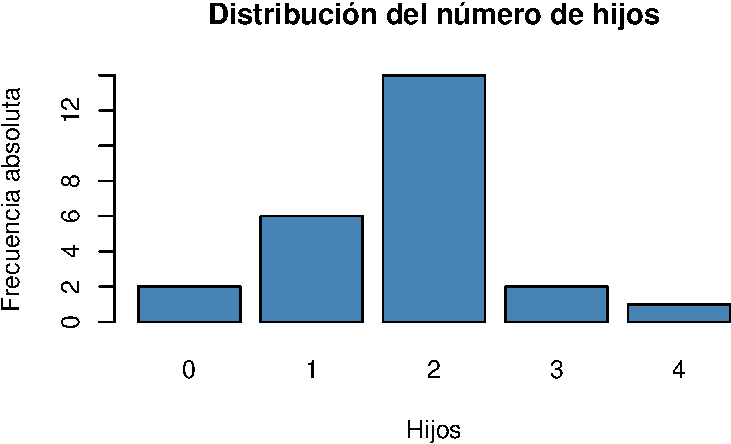
\includegraphics{03-frecuencias-graficos_files/figure-pdf/unnamed-chunk-6-1.pdf}

\begin{Shaded}
\begin{Highlighting}[]
\CommentTok{\# Diagrama de barras de frecuencias relativas.}
\FunctionTok{barplot}\NormalTok{(fi, }\AttributeTok{col =} \StringTok{"steelblue"}\NormalTok{, }\AttributeTok{main=}\StringTok{"Distribución del número de hijos"}\NormalTok{, }\AttributeTok{xlab=}\StringTok{"Hijos"}\NormalTok{, }\AttributeTok{ylab=}\StringTok{"Frecuencia relativa"}\NormalTok{)}
\end{Highlighting}
\end{Shaded}

  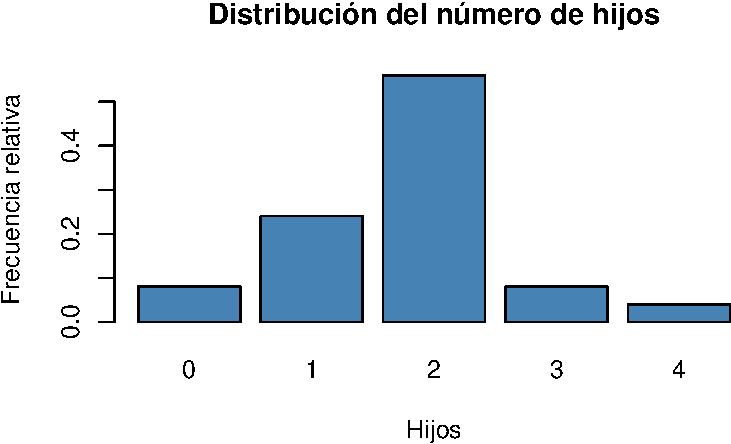
\includegraphics{03-frecuencias-graficos_files/figure-pdf/unnamed-chunk-6-2.pdf}

\begin{Shaded}
\begin{Highlighting}[]
\CommentTok{\# Diagrama de barras de frecuencias absolutas acumuladas.}
\FunctionTok{barplot}\NormalTok{(Ni, }\AttributeTok{col =} \StringTok{"steelblue"}\NormalTok{, }\AttributeTok{main=}\StringTok{"Distribución acumulada del número de hijos"}\NormalTok{, }\AttributeTok{xlab=}\StringTok{"Hijos"}\NormalTok{, }\AttributeTok{ylab=}\StringTok{"Frecuencia absoluta acumulada"}\NormalTok{)}
\end{Highlighting}
\end{Shaded}

  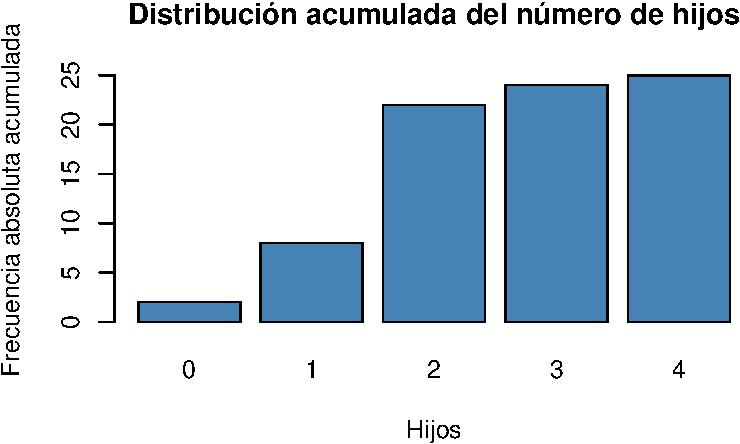
\includegraphics{03-frecuencias-graficos_files/figure-pdf/unnamed-chunk-6-3.pdf}

\begin{Shaded}
\begin{Highlighting}[]
\CommentTok{\# Diagrama de barras de frecuencias relativas acumuladas.}
\FunctionTok{barplot}\NormalTok{(Fi, }\AttributeTok{col =} \StringTok{"steelblue"}\NormalTok{, }\AttributeTok{main=}\StringTok{"Distribución acumulada del número de hijos"}\NormalTok{, }\AttributeTok{xlab=}\StringTok{"Hijos"}\NormalTok{, }\AttributeTok{ylab=}\StringTok{"Frecuencia relativa acumulada"}\NormalTok{)}
\end{Highlighting}
\end{Shaded}

  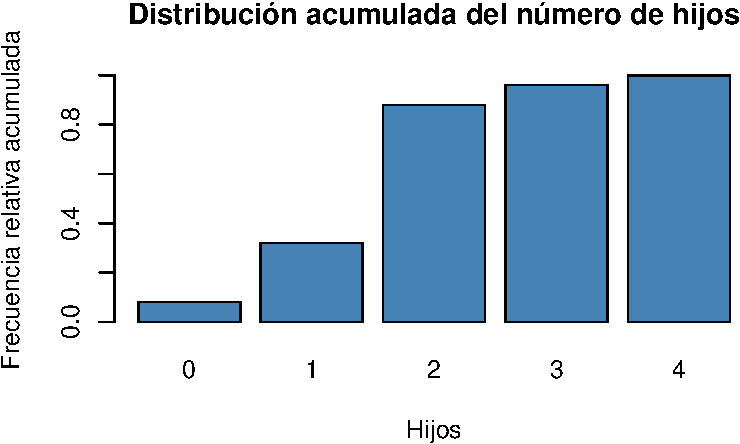
\includegraphics{03-frecuencias-graficos_files/figure-pdf/unnamed-chunk-6-4.pdf}

  \end{tcolorbox}

  \begin{tcolorbox}[enhanced jigsaw, toprule=.15mm, rightrule=.15mm, arc=.35mm, colback=white, colbacktitle=quarto-callout-tip-color!10!white, toptitle=1mm, left=2mm, colframe=quarto-callout-tip-color-frame, opacityback=0, breakable, opacitybacktitle=0.6, bottomtitle=1mm, titlerule=0mm, title=\textcolor{quarto-callout-tip-color}{\faLightbulb}\hspace{0.5em}{Solución 2}, bottomrule=.15mm, coltitle=black, leftrule=.75mm]

  Otra alternativa es usar la función la función
  \href{https://aprendeconalf.es/manual-r/07-graficos.html\#diagramas-de-barras}{\texttt{geom\_bar}}
  del paquete \texttt{ggplot2}.

\begin{Shaded}
\begin{Highlighting}[]
\FunctionTok{library}\NormalTok{(ggplot2)}
\CommentTok{\# Diagarma de barras de frecuencias absolutas}
\FunctionTok{ggplot}\NormalTok{(df, }\FunctionTok{aes}\NormalTok{(}\AttributeTok{x =}\NormalTok{ hijos)) }\SpecialCharTok{+}
    \FunctionTok{geom\_bar}\NormalTok{(}\AttributeTok{fill =} \StringTok{"steelblue"}\NormalTok{) }\SpecialCharTok{+} 
    \FunctionTok{labs}\NormalTok{(}\AttributeTok{title =} \StringTok{"Distribución del número de hijos"}\NormalTok{, }\AttributeTok{y =} \StringTok{"Frecuencia absoluta"}\NormalTok{)}
\end{Highlighting}
\end{Shaded}

  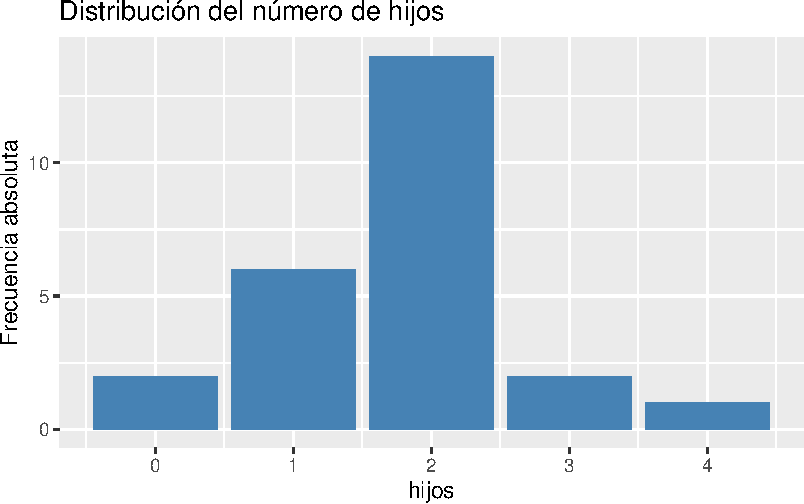
\includegraphics{03-frecuencias-graficos_files/figure-pdf/unnamed-chunk-7-1.pdf}

\begin{Shaded}
\begin{Highlighting}[]
\CommentTok{\# Diagarma de barras de frecuencias relativas}
\FunctionTok{ggplot}\NormalTok{(df, }\FunctionTok{aes}\NormalTok{(}\AttributeTok{x =}\NormalTok{ hijos)) }\SpecialCharTok{+}
    \FunctionTok{geom\_bar}\NormalTok{(}\FunctionTok{aes}\NormalTok{(}\AttributeTok{y =} \FunctionTok{after\_stat}\NormalTok{(count}\SpecialCharTok{/}\FunctionTok{sum}\NormalTok{(count))), }\AttributeTok{fill =} \StringTok{"steelblue"}\NormalTok{) }\SpecialCharTok{+}
    \FunctionTok{labs}\NormalTok{(}\AttributeTok{title =} \StringTok{"Distribución del número de hijos"}\NormalTok{, }\AttributeTok{y =} \StringTok{"Frecuencia relativa"}\NormalTok{)}
\end{Highlighting}
\end{Shaded}

  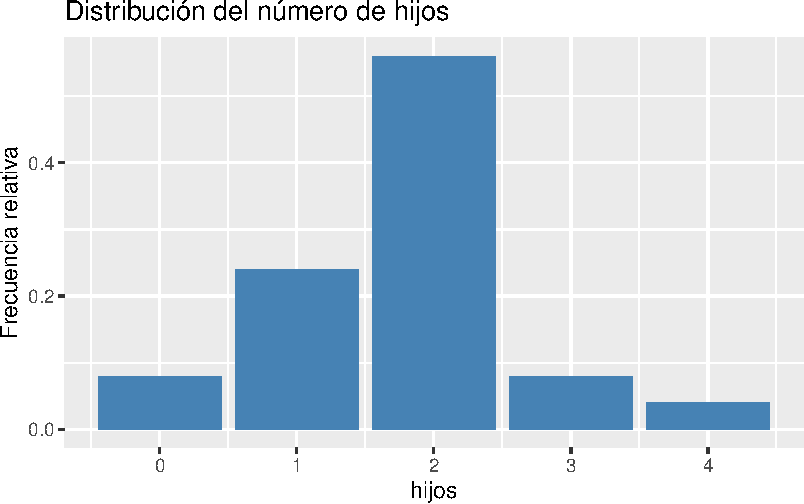
\includegraphics{03-frecuencias-graficos_files/figure-pdf/unnamed-chunk-7-2.pdf}

\begin{Shaded}
\begin{Highlighting}[]
\CommentTok{\# Diagarma de barras de frecuencias acumuladas}
\FunctionTok{ggplot}\NormalTok{(df, }\FunctionTok{aes}\NormalTok{(}\AttributeTok{x =}\NormalTok{ hijos)) }\SpecialCharTok{+}
    \FunctionTok{geom\_bar}\NormalTok{(}\FunctionTok{aes}\NormalTok{(}\AttributeTok{y =} \FunctionTok{after\_stat}\NormalTok{(}\FunctionTok{cumsum}\NormalTok{(count))), }\AttributeTok{fill =} \StringTok{"steelblue"}\NormalTok{) }\SpecialCharTok{+}
    \FunctionTok{labs}\NormalTok{(}\AttributeTok{title =} \StringTok{"Distribución acumulada del número de hijos"}\NormalTok{, }\AttributeTok{y =} \StringTok{"Frecuencia absoluta acumulada"}\NormalTok{)}
\end{Highlighting}
\end{Shaded}

  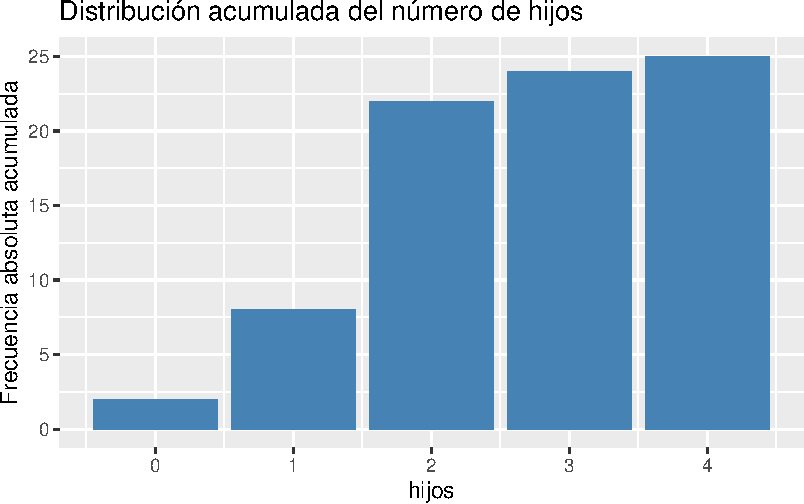
\includegraphics{03-frecuencias-graficos_files/figure-pdf/unnamed-chunk-7-3.pdf}

\begin{Shaded}
\begin{Highlighting}[]
\CommentTok{\# Diagarma de barras de frecuencias acumuladas}
\FunctionTok{ggplot}\NormalTok{(df, }\FunctionTok{aes}\NormalTok{(}\AttributeTok{x =}\NormalTok{ hijos)) }\SpecialCharTok{+}
    \FunctionTok{geom\_bar}\NormalTok{(}\FunctionTok{aes}\NormalTok{(}\AttributeTok{y =} \FunctionTok{after\_stat}\NormalTok{(}\FunctionTok{cumsum}\NormalTok{(count)}\SpecialCharTok{/}\FunctionTok{sum}\NormalTok{(count))), }\AttributeTok{fill =} \StringTok{"steelblue"}\NormalTok{) }\SpecialCharTok{+}
    \FunctionTok{labs}\NormalTok{(}\AttributeTok{title =} \StringTok{"Distribución acumulada del número de hijos"}\NormalTok{, }\AttributeTok{y =} \StringTok{"Frecuencia relativa acumulada"}\NormalTok{)}
\end{Highlighting}
\end{Shaded}

  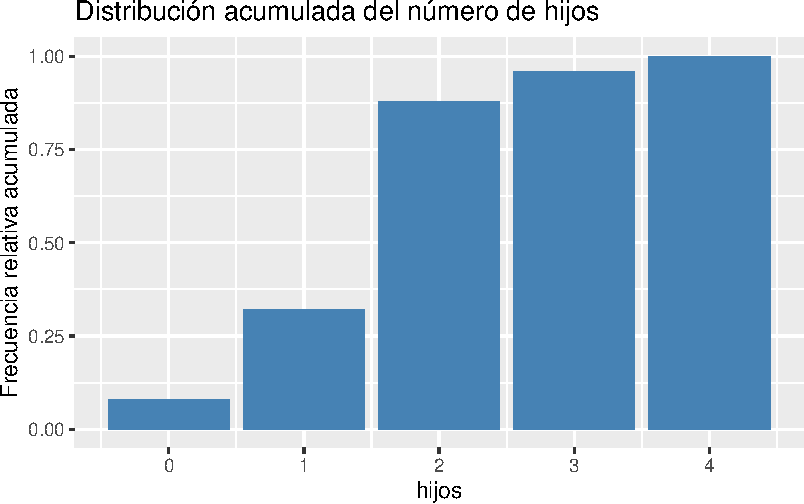
\includegraphics{03-frecuencias-graficos_files/figure-pdf/unnamed-chunk-7-4.pdf}

  \end{tcolorbox}
\item
  Dibujar el polígono de frecuencias relativas.

  \begin{tcolorbox}[enhanced jigsaw, toprule=.15mm, rightrule=.15mm, arc=.35mm, colback=white, colbacktitle=quarto-callout-tip-color!10!white, toptitle=1mm, left=2mm, colframe=quarto-callout-tip-color-frame, opacityback=0, breakable, opacitybacktitle=0.6, bottomtitle=1mm, titlerule=0mm, title=\textcolor{quarto-callout-tip-color}{\faLightbulb}\hspace{0.5em}{Solución 1}, bottomrule=.15mm, coltitle=black, leftrule=.75mm]

  Para dibujar un diagrama de lineas se puede usar la función
  \href{https://www.rdocumentation.org/packages/graphics/versions/3.6.2/topics/plot}{\texttt{plot}}
  del paquete \texttt{graphics}.

\begin{Shaded}
\begin{Highlighting}[]
\CommentTok{\# Frecuencias relativas.}
\FunctionTok{plot}\NormalTok{(}\FunctionTok{names}\NormalTok{(fi), fi, }\AttributeTok{type =} \StringTok{"l"}\NormalTok{, }\AttributeTok{col =} \StringTok{"steelblue"}\NormalTok{, }\AttributeTok{main=}\StringTok{"Distribución del número de hijos"}\NormalTok{, }\AttributeTok{xlab=}\StringTok{"Hijos"}\NormalTok{, }\AttributeTok{ylab=}\StringTok{"Frecuencia relativa"}\NormalTok{)}
\end{Highlighting}
\end{Shaded}

  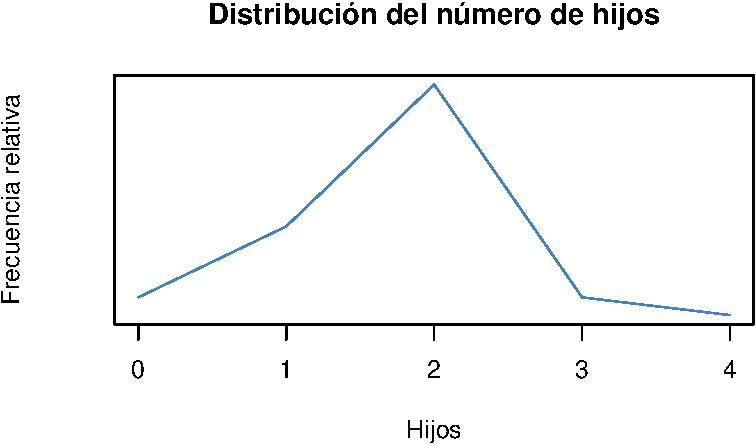
\includegraphics{03-frecuencias-graficos_files/figure-pdf/unnamed-chunk-8-1.pdf}

  \end{tcolorbox}

  \begin{tcolorbox}[enhanced jigsaw, toprule=.15mm, rightrule=.15mm, arc=.35mm, colback=white, colbacktitle=quarto-callout-tip-color!10!white, toptitle=1mm, left=2mm, colframe=quarto-callout-tip-color-frame, opacityback=0, breakable, opacitybacktitle=0.6, bottomtitle=1mm, titlerule=0mm, title=\textcolor{quarto-callout-tip-color}{\faLightbulb}\hspace{0.5em}{Solución 2}, bottomrule=.15mm, coltitle=black, leftrule=.75mm]

  Otra alternativa es usar la función la función
  \href{https://aprendeconalf.es/manual-r/07-graficos.html\#diagramas-de-lineas}{\texttt{geom\_line}}
  del paquete \texttt{ggplot2}.

\begin{Shaded}
\begin{Highlighting}[]
\FunctionTok{library}\NormalTok{(ggplot2)}
\FunctionTok{count}\NormalTok{(df, hijos) }\SpecialCharTok{|\textgreater{}} 
    \FunctionTok{mutate}\NormalTok{(}\AttributeTok{fi =}\NormalTok{ n}\SpecialCharTok{/}\FunctionTok{sum}\NormalTok{(n)) }\SpecialCharTok{|\textgreater{}}
    \FunctionTok{ggplot}\NormalTok{(}\FunctionTok{aes}\NormalTok{(}\AttributeTok{x=}\NormalTok{hijos, }\AttributeTok{y=}\NormalTok{fi)) }\SpecialCharTok{+}
    \FunctionTok{geom\_line}\NormalTok{(}\AttributeTok{col =} \StringTok{"steelblue"}\NormalTok{) }\SpecialCharTok{+}
    \FunctionTok{labs}\NormalTok{(}\AttributeTok{title =} \StringTok{"Distribución del número de hijos"}\NormalTok{, }\AttributeTok{y =} \StringTok{"Frecuencia relativa"}\NormalTok{)}
\end{Highlighting}
\end{Shaded}

  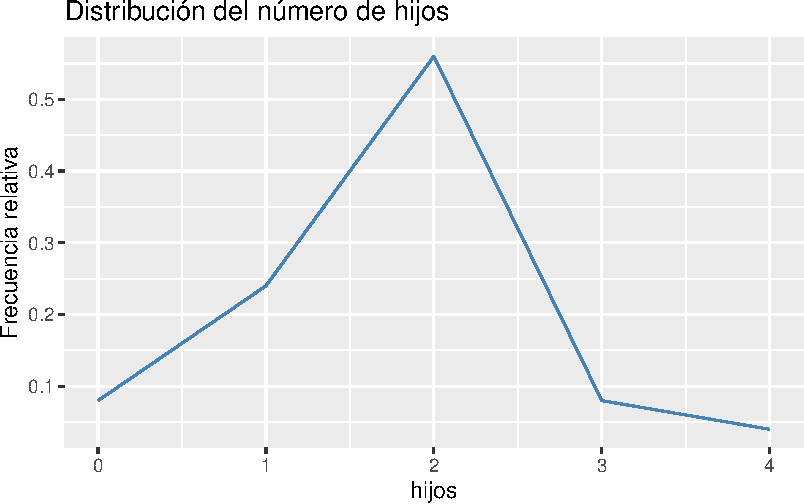
\includegraphics{03-frecuencias-graficos_files/figure-pdf/unnamed-chunk-9-1.pdf}

  \end{tcolorbox}
\end{enumerate}

\end{exercise}

\begin{exercise}[]\protect\hypertarget{exr-frecuencias-graficos-2}{}\label{exr-frecuencias-graficos-2}

En un servicio de atención al cliente se han registrado el número de
llamadas de clientes cada día del mes de noviembre, obteniendo los
siguientes datos:

\begin{longtable}[]{@{}
  >{\centering\arraybackslash}p{(\columnwidth - 0\tabcolsep) * \real{1.0000}}@{}}
\toprule\noalign{}
\endhead
\bottomrule\noalign{}
\endlastfoot
15, 23, 12, 10, 28, 50, 12, 17, 20, 21, 18, 13, 11, 12, 26, 30, 6, 16,
19, 22, 14, 17, 21, 28, 9, 16, 13, 11, 16, 20 \\
\end{longtable}

\begin{enumerate}
\def\labelenumi{\alph{enumi}.}
\item
  Crear un conjunto de datos con la variable \texttt{llamadas}.

  \begin{tcolorbox}[enhanced jigsaw, toprule=.15mm, rightrule=.15mm, arc=.35mm, colback=white, colbacktitle=quarto-callout-tip-color!10!white, toptitle=1mm, left=2mm, colframe=quarto-callout-tip-color-frame, opacityback=0, breakable, opacitybacktitle=0.6, bottomtitle=1mm, titlerule=0mm, title=\textcolor{quarto-callout-tip-color}{\faLightbulb}\hspace{0.5em}{Solución}, bottomrule=.15mm, coltitle=black, leftrule=.75mm]

\begin{Shaded}
\begin{Highlighting}[]
\NormalTok{df }\OtherTok{\textless{}{-}} \FunctionTok{data.frame}\NormalTok{(}\AttributeTok{llamadas =} \FunctionTok{c}\NormalTok{(}\DecValTok{15}\NormalTok{, }\DecValTok{23}\NormalTok{, }\DecValTok{12}\NormalTok{, }\DecValTok{10}\NormalTok{, }\DecValTok{28}\NormalTok{, }\DecValTok{50}\NormalTok{, }\DecValTok{12}\NormalTok{, }\DecValTok{17}\NormalTok{, }\DecValTok{20}\NormalTok{, }\DecValTok{21}\NormalTok{, }\DecValTok{18}\NormalTok{, }\DecValTok{13}\NormalTok{, }\DecValTok{11}\NormalTok{, }\DecValTok{12}\NormalTok{, }\DecValTok{26}\NormalTok{, }\DecValTok{30}\NormalTok{, }\DecValTok{6}\NormalTok{, }\DecValTok{16}\NormalTok{, }\DecValTok{19}\NormalTok{, }\DecValTok{22}\NormalTok{, }\DecValTok{14}\NormalTok{, }\DecValTok{17}\NormalTok{, }\DecValTok{21}\NormalTok{, }\DecValTok{28}\NormalTok{, }\DecValTok{9}\NormalTok{, }\DecValTok{16}\NormalTok{, }\DecValTok{13}\NormalTok{, }\DecValTok{11}\NormalTok{, }\DecValTok{16}\NormalTok{, }\DecValTok{20}\NormalTok{))}
\end{Highlighting}
\end{Shaded}

  \end{tcolorbox}
\item
  Dibujar el diagrama de cajas. ¿Existe algún dato atípico? En el caso
  de que exista, eliminarlo y proceder con los siguientes apartados.

  \begin{tcolorbox}[enhanced jigsaw, toprule=.15mm, rightrule=.15mm, arc=.35mm, colback=white, colbacktitle=quarto-callout-tip-color!10!white, toptitle=1mm, left=2mm, colframe=quarto-callout-tip-color-frame, opacityback=0, breakable, opacitybacktitle=0.6, bottomtitle=1mm, titlerule=0mm, title=\textcolor{quarto-callout-tip-color}{\faLightbulb}\hspace{0.5em}{Solución 1}, bottomrule=.15mm, coltitle=black, leftrule=.75mm]

  Para dibujar un diagrama de cajas se puede usar la función
  \href{https://www.rdocumentation.org/packages/graphics/versions/3.6.2/topics/boxplot}{\texttt{boxplot}}
  del paquete \texttt{graphics}.

\begin{Shaded}
\begin{Highlighting}[]
\CommentTok{\# Frecuencias relativas.}
\FunctionTok{boxplot}\NormalTok{(df}\SpecialCharTok{$}\NormalTok{llamadas, }\AttributeTok{col =} \StringTok{"steelblue"}\NormalTok{, }\AttributeTok{main=}\StringTok{"Distribución del número de llamadas"}\NormalTok{, }\AttributeTok{horizontal =}\NormalTok{ T, }\AttributeTok{xlab=}\StringTok{"Número de llamadas"}\NormalTok{)}
\end{Highlighting}
\end{Shaded}

  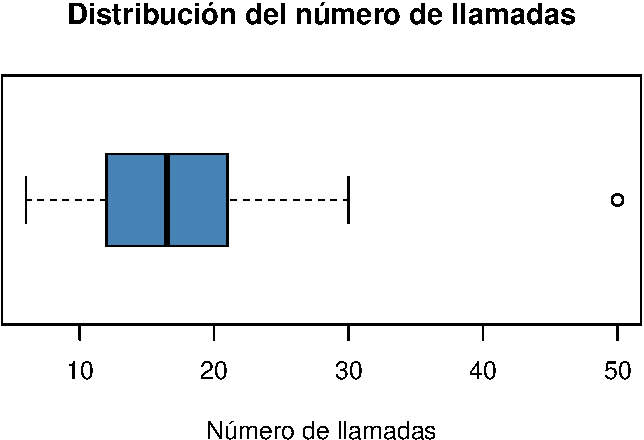
\includegraphics{03-frecuencias-graficos_files/figure-pdf/unnamed-chunk-11-1.pdf}

  \end{tcolorbox}

  \begin{tcolorbox}[enhanced jigsaw, toprule=.15mm, rightrule=.15mm, arc=.35mm, colback=white, colbacktitle=quarto-callout-tip-color!10!white, toptitle=1mm, left=2mm, colframe=quarto-callout-tip-color-frame, opacityback=0, breakable, opacitybacktitle=0.6, bottomtitle=1mm, titlerule=0mm, title=\textcolor{quarto-callout-tip-color}{\faLightbulb}\hspace{0.5em}{Solución 2}, bottomrule=.15mm, coltitle=black, leftrule=.75mm]

  Otra alternativa es usar la función la función
  \href{https://aprendeconalf.es/manual-r/07-graficos.html\#diagramas-de-cajas}{\texttt{geom\_boxplot}}
  del paquete \texttt{ggplot2}.

\begin{Shaded}
\begin{Highlighting}[]
\FunctionTok{library}\NormalTok{(ggplot2)}
\FunctionTok{ggplot}\NormalTok{(df, }\FunctionTok{aes}\NormalTok{(}\AttributeTok{x =}\NormalTok{ llamadas)) }\SpecialCharTok{+}
    \FunctionTok{geom\_boxplot}\NormalTok{(}\AttributeTok{fill =} \StringTok{"steelblue"}\NormalTok{) }\SpecialCharTok{+}
    \FunctionTok{labs}\NormalTok{(}\AttributeTok{title =} \StringTok{"Distribución del número de llamadas"}\NormalTok{, }\AttributeTok{x =} \StringTok{"Número de llamadas"}\NormalTok{)}
\end{Highlighting}
\end{Shaded}

  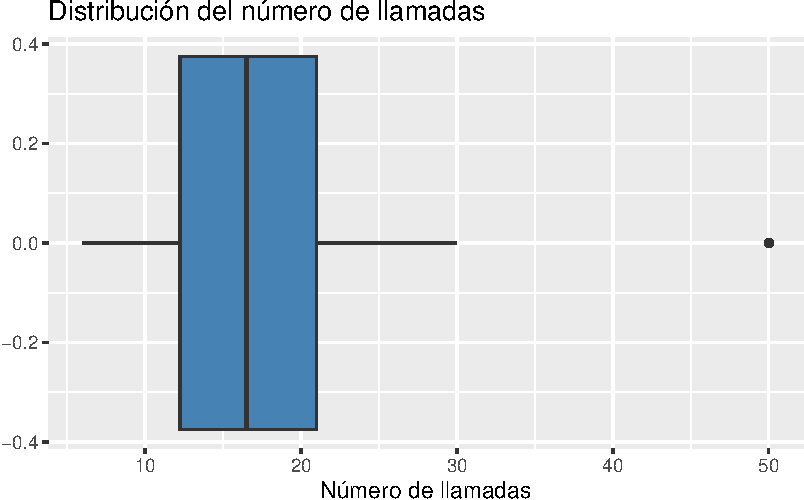
\includegraphics{03-frecuencias-graficos_files/figure-pdf/unnamed-chunk-12-1.pdf}

  Hay un día con 50 llamadas, que es un valor atípico en comparación con
  el resto de días.

  \begin{tcolorbox}[enhanced jigsaw, toprule=.15mm, rightrule=.15mm, arc=.35mm, colback=white, colbacktitle=quarto-callout-tip-color!10!white, toptitle=1mm, left=2mm, colframe=quarto-callout-tip-color-frame, opacityback=0, breakable, opacitybacktitle=0.6, bottomtitle=1mm, titlerule=0mm, title=\textcolor{quarto-callout-tip-color}{\faLightbulb}\hspace{0.5em}{Solución}, bottomrule=.15mm, coltitle=black, leftrule=.75mm]

  La función \texttt{cut}

\begin{Shaded}
\begin{Highlighting}[]
\CommentTok{\# Eliminación del dato atípico.}
\NormalTok{df }\OtherTok{\textless{}{-}}\NormalTok{ df[df}\SpecialCharTok{$}\NormalTok{llamadas }\SpecialCharTok{!=} \DecValTok{50}\NormalTok{, , drop }\OtherTok{=}\NormalTok{ F]}
\end{Highlighting}
\end{Shaded}

  \end{tcolorbox}

  \end{tcolorbox}
\item
  Construir la tabla de frecuencias agrupando en 5 clases.

  \begin{tcolorbox}[enhanced jigsaw, toprule=.15mm, rightrule=.15mm, arc=.35mm, colback=white, colbacktitle=quarto-callout-tip-color!10!white, toptitle=1mm, left=2mm, colframe=quarto-callout-tip-color-frame, opacityback=0, breakable, opacitybacktitle=0.6, bottomtitle=1mm, titlerule=0mm, title=\textcolor{quarto-callout-tip-color}{\faLightbulb}\hspace{0.5em}{Solución 1}, bottomrule=.15mm, coltitle=black, leftrule=.75mm]

  Para agrupar los datos en intervalos se puede utilizar la función
  \href{https://www.rdocumentation.org/packages/base/versions/3.6.2/topics/cut}{\texttt{cut}}
  del paquete base de R, y para contar las frecuencias absolutas y
  relativas las funciones
  \href{https://www.rdocumentation.org/packages/base/versions/3.6.2/topics/table}{\texttt{table}},
  y
  \href{https://www.rdocumentation.org/packages/base/versions/3.6.2/topics/prop.table}{\texttt{prop.table}}
  respectivamente.

\begin{Shaded}
\begin{Highlighting}[]
\CommentTok{\# Frecuencias absolutas. Creación automática de 5 clases con intervalos cerrados a la izquierda.}
\end{Highlighting}
\end{Shaded}

\begin{Shaded}
\begin{Highlighting}[]
\NormalTok{ni }\OtherTok{\textless{}{-}} \FunctionTok{table}\NormalTok{(}\FunctionTok{cut}\NormalTok{(df}\SpecialCharTok{$}\NormalTok{llamadas, }\AttributeTok{breaks =} \DecValTok{5}\NormalTok{, }\AttributeTok{right =}\NormalTok{ F))}
\CommentTok{\# Creación manual de 5 clases.}
\NormalTok{ni }\OtherTok{\textless{}{-}} \FunctionTok{table}\NormalTok{(}\FunctionTok{cut}\NormalTok{(df}\SpecialCharTok{$}\NormalTok{llamadas, }\AttributeTok{breaks =} \FunctionTok{seq}\NormalTok{(}\DecValTok{5}\NormalTok{, }\DecValTok{30}\NormalTok{, }\DecValTok{5}\NormalTok{)))}
\CommentTok{\# Frecuencias relativas}
\NormalTok{fi }\OtherTok{\textless{}{-}} \FunctionTok{prop.table}\NormalTok{(ni)}
\CommentTok{\# Frecuencias acumuladas.}
\NormalTok{Ni }\OtherTok{\textless{}{-}} \FunctionTok{cumsum}\NormalTok{(ni)}
\CommentTok{\# Frecuencias relativas acumuladas.}
\NormalTok{Fi }\OtherTok{\textless{}{-}} \FunctionTok{cumsum}\NormalTok{(fi)}
\CommentTok{\# Creación de un data frame con las frecuencias.}
\NormalTok{tabla\_frec }\OtherTok{\textless{}{-}} \FunctionTok{cbind}\NormalTok{(ni, fi, Ni, Fi)}
\NormalTok{tabla\_frec}
\end{Highlighting}
\end{Shaded}

\begin{verbatim}
        ni        fi Ni        Fi
(5,10]   3 0.1034483  3 0.1034483
(10,15]  9 0.3103448 12 0.4137931
(15,20]  9 0.3103448 21 0.7241379
(20,25]  4 0.1379310 25 0.8620690
(25,30]  4 0.1379310 29 1.0000000
\end{verbatim}

  \end{tcolorbox}

  \begin{tcolorbox}[enhanced jigsaw, toprule=.15mm, rightrule=.15mm, arc=.35mm, colback=white, colbacktitle=quarto-callout-tip-color!10!white, toptitle=1mm, left=2mm, colframe=quarto-callout-tip-color-frame, opacityback=0, breakable, opacitybacktitle=0.6, bottomtitle=1mm, titlerule=0mm, title=\textcolor{quarto-callout-tip-color}{\faLightbulb}\hspace{0.5em}{Solución 2}, bottomrule=.15mm, coltitle=black, leftrule=.75mm]

  Otra alternativa es usar la fución
  \href{https://aprendeconalf.es/manual-r/06-preprocesamiento.html\#conteo-del-n\%C3\%BAmero-de-observaciones}{\texttt{count}}
  del paquete \texttt{dplyr}.

\begin{Shaded}
\begin{Highlighting}[]
\FunctionTok{library}\NormalTok{(dplyr)}
\FunctionTok{library}\NormalTok{(knitr)}
\FunctionTok{library}\NormalTok{(kableExtra)}
\FunctionTok{mutate}\NormalTok{(df, }\AttributeTok{llamadas\_int =} \FunctionTok{cut}\NormalTok{(llamadas, }\AttributeTok{breaks =} \FunctionTok{seq}\NormalTok{(}\DecValTok{5}\NormalTok{, }\DecValTok{30}\NormalTok{, }\DecValTok{5}\NormalTok{))) }\SpecialCharTok{|\textgreater{}} 
    \FunctionTok{count}\NormalTok{(llamadas\_int) }\SpecialCharTok{|\textgreater{}}
    \FunctionTok{mutate}\NormalTok{(}\AttributeTok{fi =}\NormalTok{ n}\SpecialCharTok{/}\FunctionTok{sum}\NormalTok{(n), }\AttributeTok{Ni =} \FunctionTok{cumsum}\NormalTok{(n), }\AttributeTok{Fi =} \FunctionTok{cumsum}\NormalTok{(n)}\SpecialCharTok{/}\FunctionTok{sum}\NormalTok{(n)) }\SpecialCharTok{|\textgreater{}}
    \FunctionTok{kable}\NormalTok{()}
\end{Highlighting}
\end{Shaded}

  \begin{tabular}{l|r|r|r|r}
  \hline
  llamadas\_int & n & fi & Ni & Fi\\
  \hline
  (5,10] & 3 & 0.1034483 & 3 & 0.1034483\\
  \hline
  (10,15] & 9 & 0.3103448 & 12 & 0.4137931\\
  \hline
  (15,20] & 9 & 0.3103448 & 21 & 0.7241379\\
  \hline
  (20,25] & 4 & 0.1379310 & 25 & 0.8620690\\
  \hline
  (25,30] & 4 & 0.1379310 & 29 & 1.0000000\\
  \hline
  \end{tabular}

  \end{tcolorbox}
\item
  Dibujar el histograma de frecuencias absolutas, relativas, absolutas
  acumuladas y relativas acumuladas correspondiente a la tabla anterior.

  \begin{tcolorbox}[enhanced jigsaw, toprule=.15mm, rightrule=.15mm, arc=.35mm, colback=white, colbacktitle=quarto-callout-tip-color!10!white, toptitle=1mm, left=2mm, colframe=quarto-callout-tip-color-frame, opacityback=0, breakable, opacitybacktitle=0.6, bottomtitle=1mm, titlerule=0mm, title=\textcolor{quarto-callout-tip-color}{\faLightbulb}\hspace{0.5em}{Solución 1}, bottomrule=.15mm, coltitle=black, leftrule=.75mm]

  Para dibujar un histograma se puede usar la función
  \href{https://www.rdocumentation.org/packages/graphics/versions/3.6.2/topics/hist}{\texttt{hist}}
  del paquete \texttt{graphics}.

\begin{Shaded}
\begin{Highlighting}[]
\CommentTok{\# Histograma de frecuencias absolutas.}
\NormalTok{histo }\OtherTok{\textless{}{-}} \FunctionTok{hist}\NormalTok{(df}\SpecialCharTok{$}\NormalTok{llamadas, }\AttributeTok{breaks =} \FunctionTok{seq}\NormalTok{(}\DecValTok{5}\NormalTok{, }\DecValTok{30}\NormalTok{, }\DecValTok{5}\NormalTok{), }\AttributeTok{col =} \StringTok{"steelblue"}\NormalTok{, }\AttributeTok{main=}\StringTok{"Distribución del número de llamadas"}\NormalTok{, }\AttributeTok{xlab=}\StringTok{"Llamadas"}\NormalTok{, }\AttributeTok{ylab=}\StringTok{"Frecuencia absoluta"}\NormalTok{)}
\end{Highlighting}
\end{Shaded}

  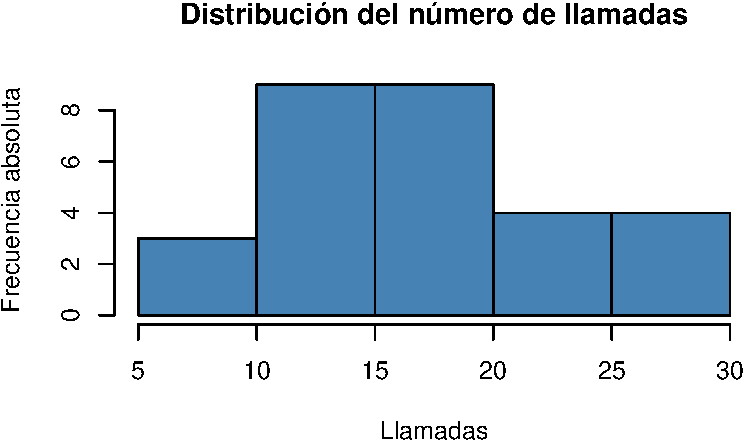
\includegraphics{03-frecuencias-graficos_files/figure-pdf/unnamed-chunk-18-1.pdf}

\begin{Shaded}
\begin{Highlighting}[]
\NormalTok{ni }\OtherTok{\textless{}{-}}\NormalTok{ histo}\SpecialCharTok{$}\NormalTok{counts}
\CommentTok{\# Histograma de frecuencias relativas.}
\NormalTok{histo}\SpecialCharTok{$}\NormalTok{counts }\OtherTok{\textless{}{-}}\NormalTok{ ni}\SpecialCharTok{/}\FunctionTok{sum}\NormalTok{(ni)}
\FunctionTok{plot}\NormalTok{(histo, }\AttributeTok{col =} \StringTok{"steelblue"}\NormalTok{, }\AttributeTok{main=}\StringTok{"Distribución del número de llamadas"}\NormalTok{, }\AttributeTok{xlab=}\StringTok{"Llamadas"}\NormalTok{, }\AttributeTok{ylab=}\StringTok{"Frecuencia relativa"}\NormalTok{)}
\end{Highlighting}
\end{Shaded}

  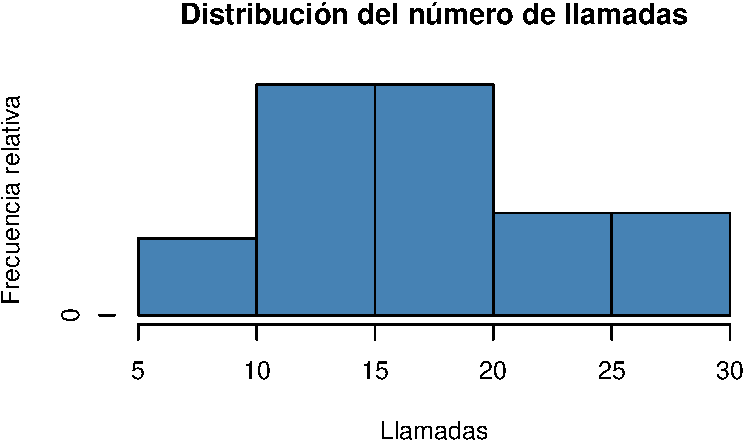
\includegraphics{03-frecuencias-graficos_files/figure-pdf/unnamed-chunk-18-2.pdf}

\begin{Shaded}
\begin{Highlighting}[]
\CommentTok{\# Histograma de frecuencias absolutas acumuladas.}
\NormalTok{histo}\SpecialCharTok{$}\NormalTok{counts }\OtherTok{\textless{}{-}} \FunctionTok{cumsum}\NormalTok{(ni)}
\FunctionTok{plot}\NormalTok{(histo, }\AttributeTok{col =} \StringTok{"steelblue"}\NormalTok{, }\AttributeTok{main=}\StringTok{"Distribución acumulada del número de llamadas"}\NormalTok{, }\AttributeTok{xlab=}\StringTok{"Llamadas"}\NormalTok{, }\AttributeTok{ylab=}\StringTok{"Frecuencia absoluta acumulada"}\NormalTok{)}
\end{Highlighting}
\end{Shaded}

  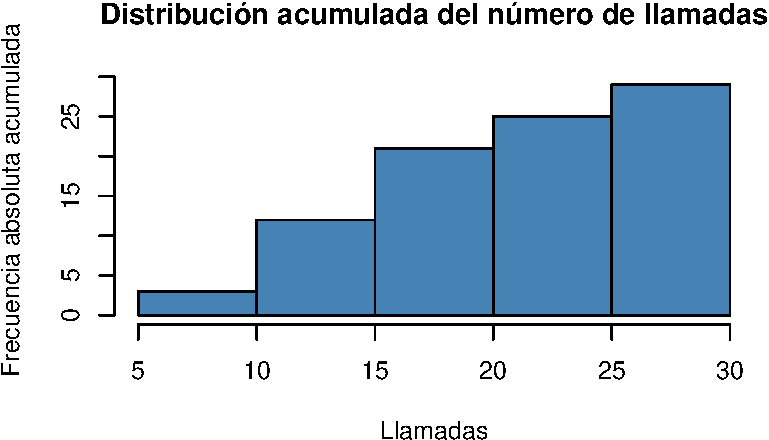
\includegraphics{03-frecuencias-graficos_files/figure-pdf/unnamed-chunk-18-3.pdf}

\begin{Shaded}
\begin{Highlighting}[]
\CommentTok{\# Histograma de frecuencias relativas acumuladas.}
\NormalTok{histo}\SpecialCharTok{$}\NormalTok{counts }\OtherTok{\textless{}{-}} \FunctionTok{cumsum}\NormalTok{(ni)}\SpecialCharTok{/}\FunctionTok{sum}\NormalTok{(ni)}
\FunctionTok{plot}\NormalTok{(histo, }\AttributeTok{col =} \StringTok{"steelblue"}\NormalTok{, }\AttributeTok{main=}\StringTok{"Distribución acumulada del número de llamadas"}\NormalTok{, }\AttributeTok{xlab=}\StringTok{"Llamadas"}\NormalTok{, }\AttributeTok{ylab=}\StringTok{"Frecuencia relativa acumulada"}\NormalTok{, )}
\end{Highlighting}
\end{Shaded}

  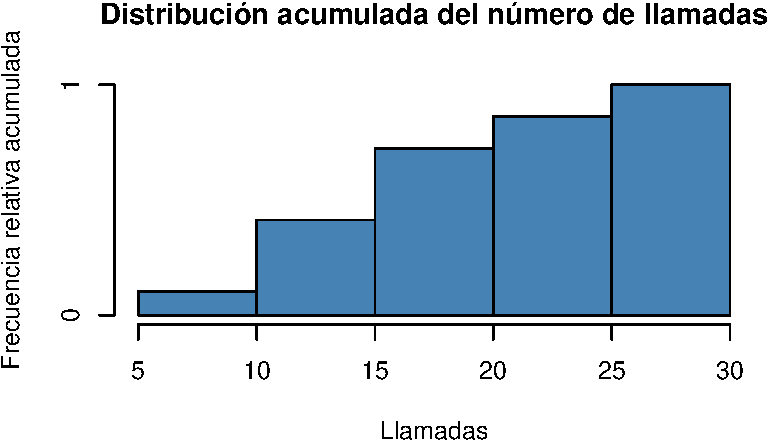
\includegraphics{03-frecuencias-graficos_files/figure-pdf/unnamed-chunk-18-4.pdf}

  \end{tcolorbox}

  \begin{tcolorbox}[enhanced jigsaw, toprule=.15mm, rightrule=.15mm, arc=.35mm, colback=white, colbacktitle=quarto-callout-tip-color!10!white, toptitle=1mm, left=2mm, colframe=quarto-callout-tip-color-frame, opacityback=0, breakable, opacitybacktitle=0.6, bottomtitle=1mm, titlerule=0mm, title=\textcolor{quarto-callout-tip-color}{\faLightbulb}\hspace{0.5em}{Solución 2}, bottomrule=.15mm, coltitle=black, leftrule=.75mm]

  Otra alternativa es usar la función la función
  \href{https://aprendeconalf.es/manual-r/07-graficos.html\#histogramas}{\texttt{geom\_histogram}}
  del paquete \texttt{ggplot2}.

\begin{Shaded}
\begin{Highlighting}[]
\FunctionTok{library}\NormalTok{(ggplot2)}
\CommentTok{\# Histograma de frecuencias absolutas}
\FunctionTok{ggplot}\NormalTok{(df, }\FunctionTok{aes}\NormalTok{(}\AttributeTok{x =}\NormalTok{ llamadas)) }\SpecialCharTok{+}
    \FunctionTok{geom\_histogram}\NormalTok{(}\AttributeTok{breaks =} \FunctionTok{seq}\NormalTok{(}\DecValTok{5}\NormalTok{, }\DecValTok{30}\NormalTok{, }\DecValTok{5}\NormalTok{), }\AttributeTok{fill =} \StringTok{"steelblue"}\NormalTok{, }\AttributeTok{col =} \StringTok{"white"}\NormalTok{) }\SpecialCharTok{+} 
    \FunctionTok{labs}\NormalTok{(}\AttributeTok{title =} \StringTok{"Distribución del número de llamadas"}\NormalTok{, }\AttributeTok{x =} \StringTok{"Número de llamadas"}\NormalTok{, }\AttributeTok{y =} \StringTok{"Frecuencia absoluta"}\NormalTok{)}
\end{Highlighting}
\end{Shaded}

  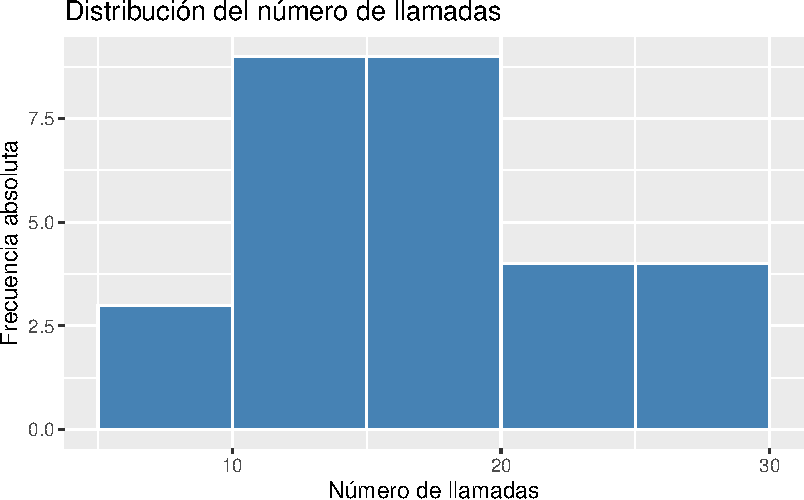
\includegraphics{03-frecuencias-graficos_files/figure-pdf/unnamed-chunk-19-1.pdf}

\begin{Shaded}
\begin{Highlighting}[]
\CommentTok{\# Histograma de frecuencias relativas}
\FunctionTok{ggplot}\NormalTok{(df, }\FunctionTok{aes}\NormalTok{(}\AttributeTok{x =}\NormalTok{ llamadas)) }\SpecialCharTok{+}
    \FunctionTok{geom\_histogram}\NormalTok{(}\FunctionTok{aes}\NormalTok{(}\AttributeTok{y =} \FunctionTok{after\_stat}\NormalTok{(count}\SpecialCharTok{/}\FunctionTok{sum}\NormalTok{(count))), }\AttributeTok{breaks =} \FunctionTok{seq}\NormalTok{(}\DecValTok{5}\NormalTok{, }\DecValTok{30}\NormalTok{, }\DecValTok{5}\NormalTok{), }\AttributeTok{fill =} \StringTok{"steelblue"}\NormalTok{, }\AttributeTok{col =} \StringTok{"white"}\NormalTok{) }\SpecialCharTok{+}
    \FunctionTok{labs}\NormalTok{(}\AttributeTok{title =} \StringTok{"Distribución del número de llamadas"}\NormalTok{, }\AttributeTok{x =} \StringTok{"Número de llamadas"}\NormalTok{, }\AttributeTok{y =} \StringTok{"Frecuencia relativa"}\NormalTok{)}
\end{Highlighting}
\end{Shaded}

  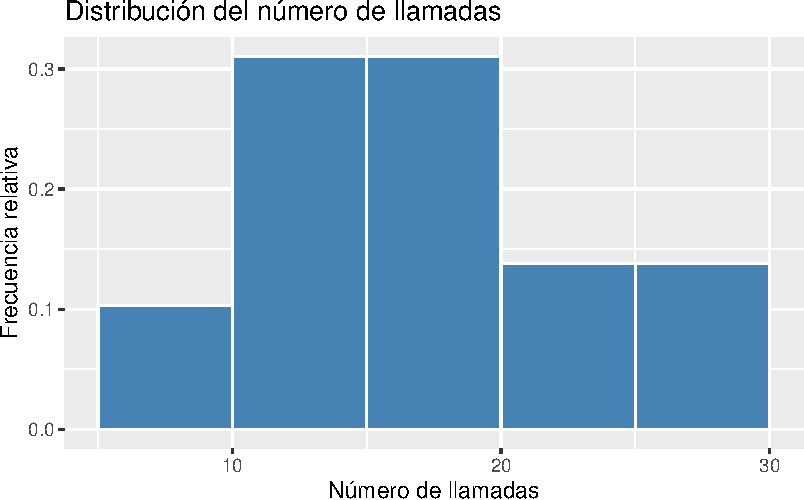
\includegraphics{03-frecuencias-graficos_files/figure-pdf/unnamed-chunk-19-2.pdf}

\begin{Shaded}
\begin{Highlighting}[]
\CommentTok{\# Histograma de frecuencias acumuladas}
\FunctionTok{ggplot}\NormalTok{(df, }\FunctionTok{aes}\NormalTok{(}\AttributeTok{x =}\NormalTok{ llamadas)) }\SpecialCharTok{+}
    \FunctionTok{geom\_histogram}\NormalTok{(}\FunctionTok{aes}\NormalTok{(}\AttributeTok{y =} \FunctionTok{after\_stat}\NormalTok{(}\FunctionTok{cumsum}\NormalTok{(count))), }\AttributeTok{breaks =} \FunctionTok{seq}\NormalTok{(}\DecValTok{5}\NormalTok{, }\DecValTok{30}\NormalTok{, }\DecValTok{5}\NormalTok{), }\AttributeTok{fill =} \StringTok{"steelblue"}\NormalTok{, }\AttributeTok{col =} \StringTok{"white"}\NormalTok{) }\SpecialCharTok{+}
    \FunctionTok{labs}\NormalTok{(}\AttributeTok{title =} \StringTok{"Distribución acumulada del número de llamadas"}\NormalTok{, }\AttributeTok{x =} \StringTok{"Número de llamadas"}\NormalTok{, }\AttributeTok{y =} \StringTok{"Frecuencia absoluta acumulada"}\NormalTok{)}
\end{Highlighting}
\end{Shaded}

  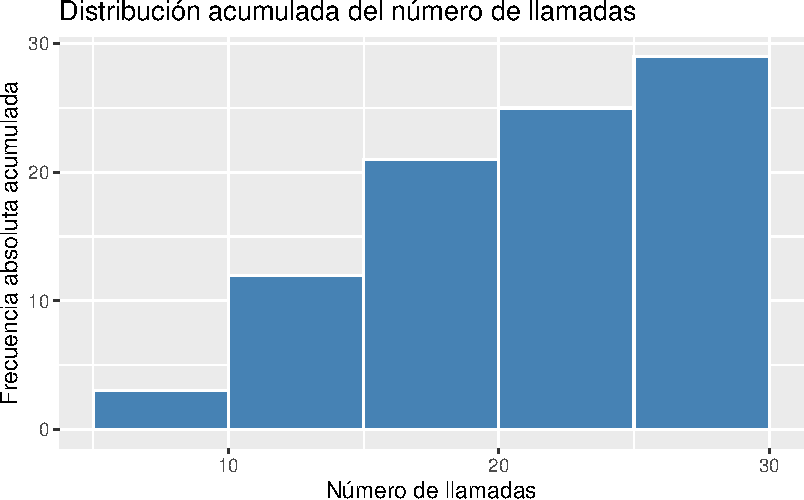
\includegraphics{03-frecuencias-graficos_files/figure-pdf/unnamed-chunk-19-3.pdf}

\begin{Shaded}
\begin{Highlighting}[]
\CommentTok{\# Histograma de frecuencias relativas acumuladas}
\FunctionTok{ggplot}\NormalTok{(df, }\FunctionTok{aes}\NormalTok{(}\AttributeTok{x =}\NormalTok{ llamadas)) }\SpecialCharTok{+}
    \FunctionTok{geom\_histogram}\NormalTok{(}\FunctionTok{aes}\NormalTok{(}\AttributeTok{y =} \FunctionTok{after\_stat}\NormalTok{(}\FunctionTok{cumsum}\NormalTok{(count)}\SpecialCharTok{/}\FunctionTok{sum}\NormalTok{(count))),  }\AttributeTok{breaks =} \FunctionTok{seq}\NormalTok{(}\DecValTok{5}\NormalTok{, }\DecValTok{30}\NormalTok{, }\DecValTok{5}\NormalTok{), }\AttributeTok{fill =} \StringTok{"steelblue"}\NormalTok{, }\AttributeTok{col =} \StringTok{"white"}\NormalTok{) }\SpecialCharTok{+}
    \FunctionTok{labs}\NormalTok{(}\AttributeTok{title =} \StringTok{"Distribución acumulada del número de llamadas"}\NormalTok{, }\AttributeTok{x =} \StringTok{"Número de llamadas"}\NormalTok{, }\AttributeTok{y =} \StringTok{"Frecuencia relativa acumulada"}\NormalTok{)}
\end{Highlighting}
\end{Shaded}

  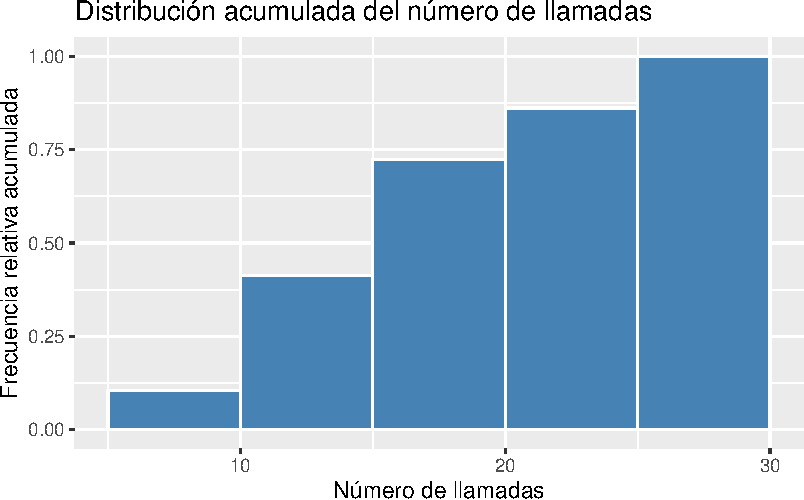
\includegraphics{03-frecuencias-graficos_files/figure-pdf/unnamed-chunk-19-4.pdf}

  \end{tcolorbox}
\item
  Dibujar el polígono de frecuencias relativas acumuladas (ojiva).

  \begin{tcolorbox}[enhanced jigsaw, toprule=.15mm, rightrule=.15mm, arc=.35mm, colback=white, colbacktitle=quarto-callout-tip-color!10!white, toptitle=1mm, left=2mm, colframe=quarto-callout-tip-color-frame, opacityback=0, breakable, opacitybacktitle=0.6, bottomtitle=1mm, titlerule=0mm, title=\textcolor{quarto-callout-tip-color}{\faLightbulb}\hspace{0.5em}{Solución 1}, bottomrule=.15mm, coltitle=black, leftrule=.75mm]

  Para dibujar la ojiva se puede usar la función
  \href{https://www.rdocumentation.org/packages/graphics/versions/3.6.2/topics/plot}{\texttt{plot}}
  del paquete \texttt{graphics}.

\begin{Shaded}
\begin{Highlighting}[]
\CommentTok{\# Ojiva}
\NormalTok{cortes }\OtherTok{=} \FunctionTok{seq}\NormalTok{(}\DecValTok{5}\NormalTok{, }\DecValTok{30}\NormalTok{, }\DecValTok{5}\NormalTok{)}
\NormalTok{ni }\OtherTok{\textless{}{-}} \FunctionTok{table}\NormalTok{(}\FunctionTok{cut}\NormalTok{(df}\SpecialCharTok{$}\NormalTok{llamadas, }\AttributeTok{breaks =}\NormalTok{ cortes))}
\NormalTok{Fi }\OtherTok{\textless{}{-}} \FunctionTok{c}\NormalTok{(}\DecValTok{0}\NormalTok{, }\FunctionTok{cumsum}\NormalTok{(ni)}\SpecialCharTok{/}\FunctionTok{sum}\NormalTok{(ni))}
\FunctionTok{plot}\NormalTok{(cortes, Fi, }\AttributeTok{type =} \StringTok{"l"}\NormalTok{, }\AttributeTok{col =} \StringTok{"steelblue"}\NormalTok{, }\AttributeTok{main =} \StringTok{"Distribución acumulada del número de llamadas"}\NormalTok{, }\AttributeTok{xlab =} \StringTok{"Número de llamadas"}\NormalTok{, }\AttributeTok{ylab =} \StringTok{"Frecuencia relativa acumulada"}\NormalTok{)}
\end{Highlighting}
\end{Shaded}

  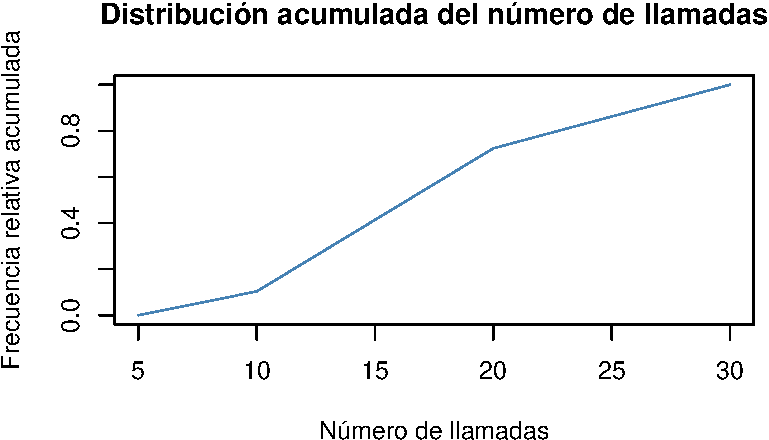
\includegraphics{03-frecuencias-graficos_files/figure-pdf/unnamed-chunk-20-1.pdf}

  \end{tcolorbox}

  \begin{tcolorbox}[enhanced jigsaw, toprule=.15mm, rightrule=.15mm, arc=.35mm, colback=white, colbacktitle=quarto-callout-tip-color!10!white, toptitle=1mm, left=2mm, colframe=quarto-callout-tip-color-frame, opacityback=0, breakable, opacitybacktitle=0.6, bottomtitle=1mm, titlerule=0mm, title=\textcolor{quarto-callout-tip-color}{\faLightbulb}\hspace{0.5em}{Solución 2}, bottomrule=.15mm, coltitle=black, leftrule=.75mm]

  Otra alternativa es usar la función la función
  \href{https://aprendeconalf.es/manual-r/07-graficos.html\#histogramas}{\texttt{geom\_line}}
  del paquete \texttt{ggplot2}.

\begin{Shaded}
\begin{Highlighting}[]
\FunctionTok{library}\NormalTok{(ggplot2)}
\CommentTok{\# Ojiva}
\NormalTok{cortes }\OtherTok{\textless{}{-}} \FunctionTok{seq}\NormalTok{(}\DecValTok{5}\NormalTok{, }\DecValTok{30}\NormalTok{, }\DecValTok{5}\NormalTok{)}
\NormalTok{tabla\_frec }\OtherTok{\textless{}{-}} \FunctionTok{mutate}\NormalTok{(df, }\AttributeTok{llamadas\_int =} \FunctionTok{cut}\NormalTok{(df}\SpecialCharTok{$}\NormalTok{llamadas, }\AttributeTok{breaks =}\NormalTok{ cortes)) }\SpecialCharTok{|\textgreater{}} 
    \FunctionTok{count}\NormalTok{(llamadas\_int) }\SpecialCharTok{|\textgreater{}}
    \FunctionTok{mutate}\NormalTok{(}\AttributeTok{cortes =}\NormalTok{ cortes[}\SpecialCharTok{{-}}\DecValTok{1}\NormalTok{], }\AttributeTok{Fi =} \FunctionTok{cumsum}\NormalTok{(n)}\SpecialCharTok{/}\FunctionTok{sum}\NormalTok{(n)) }\SpecialCharTok{|\textgreater{}}
    \FunctionTok{select}\NormalTok{(cortes, Fi) }
\NormalTok{tabla\_frec }\OtherTok{\textless{}{-}} \FunctionTok{rbind}\NormalTok{(}\FunctionTok{data.frame}\NormalTok{(}\AttributeTok{cortes =}\NormalTok{ cortes[}\DecValTok{1}\NormalTok{], }\AttributeTok{Fi =} \DecValTok{0}\NormalTok{), tabla\_frec)}
\FunctionTok{ggplot}\NormalTok{(tabla\_frec, }\FunctionTok{aes}\NormalTok{(}\AttributeTok{x =}\NormalTok{ cortes , }\AttributeTok{y =}\NormalTok{ Fi)) }\SpecialCharTok{+}
    \FunctionTok{geom\_line}\NormalTok{(}\AttributeTok{col =} \StringTok{"steelblue"}\NormalTok{) }\SpecialCharTok{+}
    \FunctionTok{labs}\NormalTok{(}\AttributeTok{title =} \StringTok{"Distribución del número de llamadas"}\NormalTok{, }\AttributeTok{x =} \StringTok{"Número de llamadas"}\NormalTok{, }\AttributeTok{y =} \StringTok{"Frecuencia relativa acumulada"}\NormalTok{)}
\end{Highlighting}
\end{Shaded}

  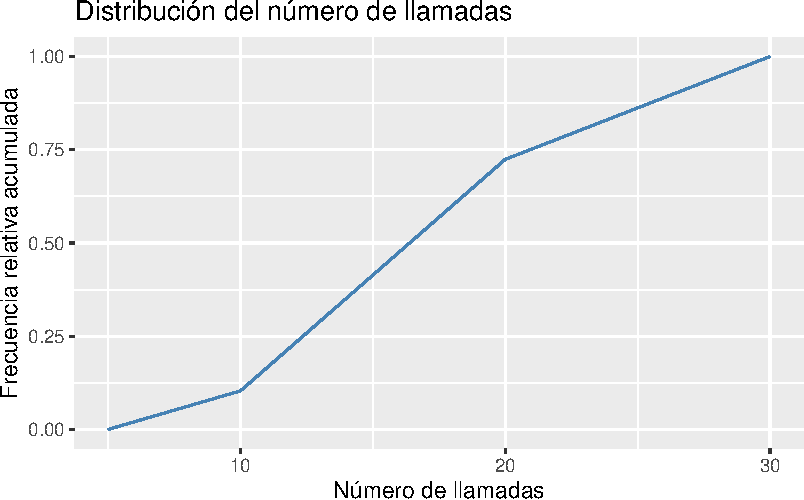
\includegraphics{03-frecuencias-graficos_files/figure-pdf/unnamed-chunk-21-1.pdf}

  \end{tcolorbox}
\end{enumerate}

\end{exercise}

\begin{exercise}[]\protect\hypertarget{exr-frecuencias-graficos-3}{}\label{exr-frecuencias-graficos-3}

Los grupos sanguíneos de una muestra de 30 personas son:

\begin{longtable}[]{@{}
  >{\centering\arraybackslash}p{(\columnwidth - 0\tabcolsep) * \real{1.0000}}@{}}
\toprule\noalign{}
\endhead
\bottomrule\noalign{}
\endlastfoot
A, B, B, A, AB, 0, 0, A, B, B, A, A, A, A, AB, A, A, A, B, 0, B, B, B,
A, A, A, 0, A, AB, 0 \\
\end{longtable}

\begin{enumerate}
\def\labelenumi{\alph{enumi}.}
\item
  Crear un conjunto de datos con la variable \texttt{grupo\_sanguíneo}.

  \begin{tcolorbox}[enhanced jigsaw, toprule=.15mm, rightrule=.15mm, arc=.35mm, colback=white, colbacktitle=quarto-callout-tip-color!10!white, toptitle=1mm, left=2mm, colframe=quarto-callout-tip-color-frame, opacityback=0, breakable, opacitybacktitle=0.6, bottomtitle=1mm, titlerule=0mm, title=\textcolor{quarto-callout-tip-color}{\faLightbulb}\hspace{0.5em}{Solución}, bottomrule=.15mm, coltitle=black, leftrule=.75mm]

\begin{Shaded}
\begin{Highlighting}[]
\NormalTok{df }\OtherTok{\textless{}{-}} \FunctionTok{data.frame}\NormalTok{(}\AttributeTok{grupo\_sanguineo =} \FunctionTok{c}\NormalTok{(}\StringTok{"A"}\NormalTok{, }\StringTok{"B"}\NormalTok{, }\StringTok{"B"}\NormalTok{, }\StringTok{"A"}\NormalTok{, }\StringTok{"AB"}\NormalTok{, }\StringTok{"0"}\NormalTok{, }\StringTok{"0"}\NormalTok{, }\StringTok{"A"}\NormalTok{, }\StringTok{"B"}\NormalTok{, }\StringTok{"B"}\NormalTok{, }\StringTok{"A"}\NormalTok{, }\StringTok{"A"}\NormalTok{, }\StringTok{"A"}\NormalTok{, }\StringTok{"A"}\NormalTok{, }\StringTok{"AB"}\NormalTok{, }\StringTok{"A"}\NormalTok{, }\StringTok{"A"}\NormalTok{, }\StringTok{"A"}\NormalTok{, }\StringTok{"B"}\NormalTok{, }\StringTok{"0"}\NormalTok{, }\StringTok{"B"}\NormalTok{, }\StringTok{"B"}\NormalTok{, }\StringTok{"B"}\NormalTok{, }\StringTok{"A"}\NormalTok{, }\StringTok{"A"}\NormalTok{, }\StringTok{"A"}\NormalTok{, }\StringTok{"0"}\NormalTok{, }\StringTok{"A"}\NormalTok{, }\StringTok{"AB"}\NormalTok{, }\StringTok{"0"}\NormalTok{))}
\end{Highlighting}
\end{Shaded}

  \end{tcolorbox}
\item
  Construir la tabla de frecuencias.

  \begin{tcolorbox}[enhanced jigsaw, toprule=.15mm, rightrule=.15mm, arc=.35mm, colback=white, colbacktitle=quarto-callout-tip-color!10!white, toptitle=1mm, left=2mm, colframe=quarto-callout-tip-color-frame, opacityback=0, breakable, opacitybacktitle=0.6, bottomtitle=1mm, titlerule=0mm, title=\textcolor{quarto-callout-tip-color}{\faLightbulb}\hspace{0.5em}{Solución 1}, bottomrule=.15mm, coltitle=black, leftrule=.75mm]

  Para obtener las frecuencias absolutas se puede usar la función
  \href{https://www.rdocumentation.org/packages/base/versions/3.6.2/topics/table}{\texttt{table}},
  y para las frecuencias relativas la función
  \href{https://www.rdocumentation.org/packages/base/versions/3.6.2/topics/prop.table}{\texttt{prop.table}}
  ambas del paquete base de R.

\begin{Shaded}
\begin{Highlighting}[]
\CommentTok{\# Frecuencias absolutas.}
\NormalTok{ni }\OtherTok{\textless{}{-}} \FunctionTok{table}\NormalTok{(df}\SpecialCharTok{$}\NormalTok{grupo\_sanguineo)}
\CommentTok{\# Frecuencias relativas}
\NormalTok{fi }\OtherTok{\textless{}{-}} \FunctionTok{prop.table}\NormalTok{(ni)}
\NormalTok{tabla\_frec }\OtherTok{\textless{}{-}} \FunctionTok{cbind}\NormalTok{(ni, fi)}
\NormalTok{tabla\_frec}
\end{Highlighting}
\end{Shaded}

\begin{verbatim}
   ni        fi
0   5 0.1666667
A  14 0.4666667
AB  3 0.1000000
B   8 0.2666667
\end{verbatim}

  \end{tcolorbox}

  \begin{tcolorbox}[enhanced jigsaw, toprule=.15mm, rightrule=.15mm, arc=.35mm, colback=white, colbacktitle=quarto-callout-tip-color!10!white, toptitle=1mm, left=2mm, colframe=quarto-callout-tip-color-frame, opacityback=0, breakable, opacitybacktitle=0.6, bottomtitle=1mm, titlerule=0mm, title=\textcolor{quarto-callout-tip-color}{\faLightbulb}\hspace{0.5em}{Solución 2}, bottomrule=.15mm, coltitle=black, leftrule=.75mm]

  Otra alternativa es usar la fución
  \href{https://aprendeconalf.es/manual-r/06-preprocesamiento.html\#conteo-del-n\%C3\%BAmero-de-observaciones}{\texttt{count}}
  del paquete \texttt{dplyr}.

\begin{Shaded}
\begin{Highlighting}[]
\FunctionTok{library}\NormalTok{(dplyr)}
\FunctionTok{library}\NormalTok{(knitr)}
\FunctionTok{library}\NormalTok{(kableExtra)}
\FunctionTok{count}\NormalTok{(df, grupo\_sanguineo) }\SpecialCharTok{|\textgreater{}} 
    \FunctionTok{mutate}\NormalTok{(}\AttributeTok{fi =}\NormalTok{ n}\SpecialCharTok{/}\FunctionTok{sum}\NormalTok{(n)) }\SpecialCharTok{|\textgreater{}}
    \FunctionTok{kable}\NormalTok{()}
\end{Highlighting}
\end{Shaded}

  \begin{tabular}{l|r|r}
  \hline
  grupo\_sanguineo & n & fi\\
  \hline
  0 & 5 & 0.1666667\\
  \hline
  A & 14 & 0.4666667\\
  \hline
  AB & 3 & 0.1000000\\
  \hline
  B & 8 & 0.2666667\\
  \hline
  \end{tabular}

  \end{tcolorbox}
\item
  Dibujar el diagrama de sectores.

  \begin{tcolorbox}[enhanced jigsaw, toprule=.15mm, rightrule=.15mm, arc=.35mm, colback=white, colbacktitle=quarto-callout-tip-color!10!white, toptitle=1mm, left=2mm, colframe=quarto-callout-tip-color-frame, opacityback=0, breakable, opacitybacktitle=0.6, bottomtitle=1mm, titlerule=0mm, title=\textcolor{quarto-callout-tip-color}{\faLightbulb}\hspace{0.5em}{Solución 1}, bottomrule=.15mm, coltitle=black, leftrule=.75mm]

  Para dibujar el diagrama de sectores se puede usar la función
  \href{https://www.rdocumentation.org/packages/graphics/versions/3.6.2/topics/pie}{\texttt{pie}}
  del paquete \texttt{graphics}.

\begin{Shaded}
\begin{Highlighting}[]
\CommentTok{\# Diagrama de sectores}
\FunctionTok{pie}\NormalTok{(ni, }\AttributeTok{col =} \DecValTok{1}\SpecialCharTok{:}\FunctionTok{length}\NormalTok{(ni), }\AttributeTok{main =} \StringTok{"Distribución de los grupos sanguíneos"}\NormalTok{)}
\end{Highlighting}
\end{Shaded}

  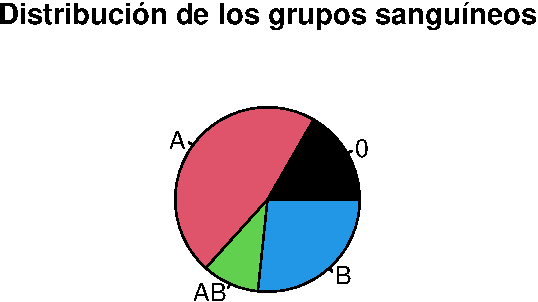
\includegraphics{03-frecuencias-graficos_files/figure-pdf/unnamed-chunk-26-1.pdf}

  \end{tcolorbox}

  \begin{tcolorbox}[enhanced jigsaw, toprule=.15mm, rightrule=.15mm, arc=.35mm, colback=white, colbacktitle=quarto-callout-tip-color!10!white, toptitle=1mm, left=2mm, colframe=quarto-callout-tip-color-frame, opacityback=0, breakable, opacitybacktitle=0.6, bottomtitle=1mm, titlerule=0mm, title=\textcolor{quarto-callout-tip-color}{\faLightbulb}\hspace{0.5em}{Solución 2}, bottomrule=.15mm, coltitle=black, leftrule=.75mm]

  Otra alternativa es usar las fuciones
  \href{https://aprendeconalf.es/manual-r/07-graficos.html\#diagrama-de-sectores}{\texttt{geom\_bar}}
  y \texttt{coor\_polar} del paquete \texttt{ggplot2}.

\begin{Shaded}
\begin{Highlighting}[]
\FunctionTok{ggplot}\NormalTok{(df, }\FunctionTok{aes}\NormalTok{(}\AttributeTok{x =} \StringTok{""}\NormalTok{, }\AttributeTok{fill =}\NormalTok{ grupo\_sanguineo)) }\SpecialCharTok{+}
    \CommentTok{\# Añadir la capa de las barras.}
    \FunctionTok{geom\_bar}\NormalTok{() }\SpecialCharTok{+}
    \CommentTok{\# Añadir el sistema de coordenadas polares}
    \FunctionTok{coord\_polar}\NormalTok{(}\AttributeTok{theta =} \StringTok{"y"}\NormalTok{) }\SpecialCharTok{+}
    \FunctionTok{labs}\NormalTok{(}\AttributeTok{title =} \StringTok{"Distribución de los grupos sanguíneos"}\NormalTok{)}
\end{Highlighting}
\end{Shaded}

  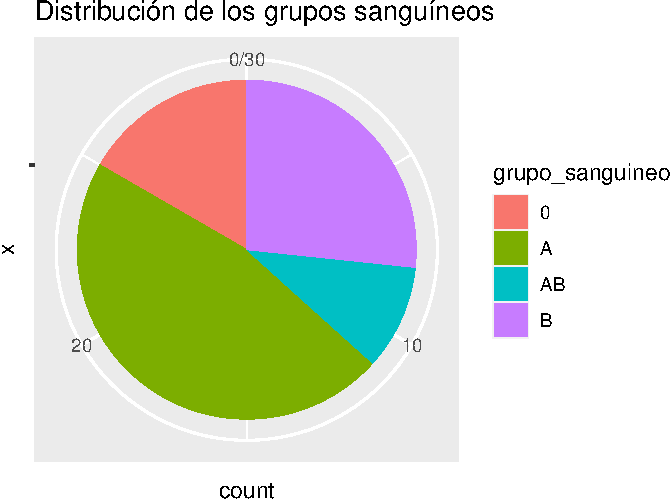
\includegraphics{03-frecuencias-graficos_files/figure-pdf/unnamed-chunk-27-1.pdf}

  \end{tcolorbox}
\end{enumerate}

\end{exercise}

\begin{exercise}[]\protect\hypertarget{exr-frecuencias-graficos-4}{}\label{exr-frecuencias-graficos-4}

En un estudio de población se tomó una muestra de 27 personas, y se les
preguntó por su edad y estado civil, obteniendo los siguientes
resultados:

\begin{longtable}[]{@{}ll@{}}
\toprule\noalign{}
Estado civil & Edad \\
\midrule\noalign{}
\endhead
\bottomrule\noalign{}
\endlastfoot
Soltero & 31, 45, 35, 65, 21, 38, 62, 22, 31 \\
Casado & 62, 39, 62, 59, 21, 62 \\
Viudo & 80, 68, 65, 40, 78, 69, 75 \\
Divorciado & 31, 65, 59, 49, 65 \\
\end{longtable}

\begin{enumerate}
\def\labelenumi{\alph{enumi}.}
\item
  Crear un conjunto de datos con la variables \texttt{estado\_civil} y
  \texttt{edad}.

  \begin{tcolorbox}[enhanced jigsaw, toprule=.15mm, rightrule=.15mm, arc=.35mm, colback=white, colbacktitle=quarto-callout-tip-color!10!white, toptitle=1mm, left=2mm, colframe=quarto-callout-tip-color-frame, opacityback=0, breakable, opacitybacktitle=0.6, bottomtitle=1mm, titlerule=0mm, title=\textcolor{quarto-callout-tip-color}{\faLightbulb}\hspace{0.5em}{Solución}, bottomrule=.15mm, coltitle=black, leftrule=.75mm]

\begin{Shaded}
\begin{Highlighting}[]
\NormalTok{df }\OtherTok{\textless{}{-}} \FunctionTok{data.frame}\NormalTok{(}
    \AttributeTok{edad =} \FunctionTok{c}\NormalTok{(}\DecValTok{31}\NormalTok{, }\DecValTok{45}\NormalTok{, }\DecValTok{35}\NormalTok{, }\DecValTok{65}\NormalTok{, }\DecValTok{21}\NormalTok{, }\DecValTok{38}\NormalTok{, }\DecValTok{62}\NormalTok{, }\DecValTok{22}\NormalTok{, }\DecValTok{31}\NormalTok{, }\DecValTok{62}\NormalTok{, }\DecValTok{39}\NormalTok{, }\DecValTok{62}\NormalTok{, }\DecValTok{59}\NormalTok{, }\DecValTok{21}\NormalTok{, }\DecValTok{62}\NormalTok{, }\DecValTok{80}\NormalTok{, }\DecValTok{68}\NormalTok{, }\DecValTok{65}\NormalTok{, }\DecValTok{40}\NormalTok{, }\DecValTok{78}\NormalTok{, }\DecValTok{69}\NormalTok{, }\DecValTok{75}\NormalTok{, }\DecValTok{31}\NormalTok{, }\DecValTok{65}\NormalTok{, }\DecValTok{59}\NormalTok{, }\DecValTok{49}\NormalTok{, }\DecValTok{65}\NormalTok{), }
    \AttributeTok{estado\_civil =} \FunctionTok{rep}\NormalTok{(}\FunctionTok{c}\NormalTok{(}\StringTok{"Soltero"}\NormalTok{, }\StringTok{"Casado"}\NormalTok{, }\StringTok{"Viudo"}\NormalTok{, }\StringTok{"Divorciado"}\NormalTok{), }\FunctionTok{c}\NormalTok{(}\DecValTok{9}\NormalTok{, }\DecValTok{6}\NormalTok{, }\DecValTok{7}\NormalTok{, }\DecValTok{5}\NormalTok{)))}
\end{Highlighting}
\end{Shaded}

  \end{tcolorbox}
\item
  Calcular los tamaños muestrales según \texttt{estado\_civil}.

  \begin{tcolorbox}[enhanced jigsaw, toprule=.15mm, rightrule=.15mm, arc=.35mm, colback=white, colbacktitle=quarto-callout-tip-color!10!white, toptitle=1mm, left=2mm, colframe=quarto-callout-tip-color-frame, opacityback=0, breakable, opacitybacktitle=0.6, bottomtitle=1mm, titlerule=0mm, title=\textcolor{quarto-callout-tip-color}{\faLightbulb}\hspace{0.5em}{Solución 1}, bottomrule=.15mm, coltitle=black, leftrule=.75mm]

  Usando la función \texttt{table} del paquete base de R podemos obtener
  las frecuencias absolutas del estado civil que es el tamaño muestral
  de cada grupo.

\begin{Shaded}
\begin{Highlighting}[]
\FunctionTok{table}\NormalTok{(df}\SpecialCharTok{$}\NormalTok{estado\_civil)}
\end{Highlighting}
\end{Shaded}

\begin{verbatim}

    Casado Divorciado    Soltero      Viudo 
         6          5          9          7 
\end{verbatim}

  \end{tcolorbox}

  \begin{tcolorbox}[enhanced jigsaw, toprule=.15mm, rightrule=.15mm, arc=.35mm, colback=white, colbacktitle=quarto-callout-tip-color!10!white, toptitle=1mm, left=2mm, colframe=quarto-callout-tip-color-frame, opacityback=0, breakable, opacitybacktitle=0.6, bottomtitle=1mm, titlerule=0mm, title=\textcolor{quarto-callout-tip-color}{\faLightbulb}\hspace{0.5em}{Solución 2}, bottomrule=.15mm, coltitle=black, leftrule=.75mm]

  Usando las funciones \texttt{groub\_by}, \texttt{summarise} y
  \texttt{n} del paquete \texttt{dplyr}.

\begin{Shaded}
\begin{Highlighting}[]
\FunctionTok{library}\NormalTok{(dplyr)}
\NormalTok{df }\SpecialCharTok{|\textgreater{}} \FunctionTok{group\_by}\NormalTok{(estado\_civil) }\SpecialCharTok{|\textgreater{}}
    \FunctionTok{summarise}\NormalTok{(}\AttributeTok{n =} \FunctionTok{n}\NormalTok{())}
\end{Highlighting}
\end{Shaded}

\begin{verbatim}
# A tibble: 4 x 2
  estado_civil     n
  <chr>        <int>
1 Casado           6
2 Divorciado       5
3 Soltero          9
4 Viudo            7
\end{verbatim}

  \end{tcolorbox}
\item
  Construir la tabla de frecuencias de la variable \texttt{edad} para
  cada categoría de la variable \texttt{estado\_civil}.

  \begin{tcolorbox}[enhanced jigsaw, toprule=.15mm, rightrule=.15mm, arc=.35mm, colback=white, colbacktitle=quarto-callout-tip-color!10!white, toptitle=1mm, left=2mm, colframe=quarto-callout-tip-color-frame, opacityback=0, breakable, opacitybacktitle=0.6, bottomtitle=1mm, titlerule=0mm, title=\textcolor{quarto-callout-tip-color}{\faLightbulb}\hspace{0.5em}{Solución}, bottomrule=.15mm, coltitle=black, leftrule=.75mm]

  Para dividir la muestra en grupos se puede usar la función
  \href{https://aprendeconalf.es/manual-r/06-preprocesamiento.html\#res\%C3\%BAmenes-por-grupos}{\texttt{group-by}}
  del paquete \texttt{dplyr}.

\begin{Shaded}
\begin{Highlighting}[]
\FunctionTok{library}\NormalTok{(dplyr)}
\FunctionTok{library}\NormalTok{(knitr)}
\FunctionTok{library}\NormalTok{(kableExtra)}
\FunctionTok{mutate}\NormalTok{(df, }\AttributeTok{edad\_int =} \FunctionTok{cut}\NormalTok{(edad, }\AttributeTok{breaks =} \FunctionTok{seq}\NormalTok{(}\DecValTok{20}\NormalTok{, }\DecValTok{80}\NormalTok{, }\DecValTok{10}\NormalTok{))) }\SpecialCharTok{|\textgreater{}}
    \FunctionTok{group\_by}\NormalTok{(estado\_civil) }\SpecialCharTok{|\textgreater{}}
    \FunctionTok{count}\NormalTok{(edad\_int) }\SpecialCharTok{|\textgreater{}} 
    \FunctionTok{mutate}\NormalTok{(}\AttributeTok{fi =}\NormalTok{ n}\SpecialCharTok{/}\FunctionTok{sum}\NormalTok{(n), }\AttributeTok{Ni =} \FunctionTok{cumsum}\NormalTok{(n), }\AttributeTok{Fi =} \FunctionTok{cumsum}\NormalTok{(n)}\SpecialCharTok{/}\FunctionTok{sum}\NormalTok{(n)) }\SpecialCharTok{|\textgreater{}}
    \FunctionTok{kable}\NormalTok{()}
\end{Highlighting}
\end{Shaded}

  \begin{tabular}{l|l|r|r|r|r}
  \hline
  estado\_civil & edad\_int & n & fi & Ni & Fi\\
  \hline
  Casado & (20,30] & 1 & 0.1666667 & 1 & 0.1666667\\
  \hline
  Casado & (30,40] & 1 & 0.1666667 & 2 & 0.3333333\\
  \hline
  Casado & (50,60] & 1 & 0.1666667 & 3 & 0.5000000\\
  \hline
  Casado & (60,70] & 3 & 0.5000000 & 6 & 1.0000000\\
  \hline
  Divorciado & (30,40] & 1 & 0.2000000 & 1 & 0.2000000\\
  \hline
  Divorciado & (40,50] & 1 & 0.2000000 & 2 & 0.4000000\\
  \hline
  Divorciado & (50,60] & 1 & 0.2000000 & 3 & 0.6000000\\
  \hline
  Divorciado & (60,70] & 2 & 0.4000000 & 5 & 1.0000000\\
  \hline
  Soltero & (20,30] & 2 & 0.2222222 & 2 & 0.2222222\\
  \hline
  Soltero & (30,40] & 4 & 0.4444444 & 6 & 0.6666667\\
  \hline
  Soltero & (40,50] & 1 & 0.1111111 & 7 & 0.7777778\\
  \hline
  Soltero & (60,70] & 2 & 0.2222222 & 9 & 1.0000000\\
  \hline
  Viudo & (30,40] & 1 & 0.1428571 & 1 & 0.1428571\\
  \hline
  Viudo & (60,70] & 3 & 0.4285714 & 4 & 0.5714286\\
  \hline
  Viudo & (70,80] & 3 & 0.4285714 & 7 & 1.0000000\\
  \hline
  \end{tabular}

  \end{tcolorbox}
\item
  Dibujar los diagramas de cajas de la edad según el estado civil.
  ¿Existen datos atípicos? ¿En qué grupo hay mayor dispersión?

  \begin{tcolorbox}[enhanced jigsaw, toprule=.15mm, rightrule=.15mm, arc=.35mm, colback=white, colbacktitle=quarto-callout-tip-color!10!white, toptitle=1mm, left=2mm, colframe=quarto-callout-tip-color-frame, opacityback=0, breakable, opacitybacktitle=0.6, bottomtitle=1mm, titlerule=0mm, title=\textcolor{quarto-callout-tip-color}{\faLightbulb}\hspace{0.5em}{Solución}, bottomrule=.15mm, coltitle=black, leftrule=.75mm]

\begin{Shaded}
\begin{Highlighting}[]
\FunctionTok{library}\NormalTok{(ggplot2)}
\FunctionTok{ggplot}\NormalTok{(df, }\FunctionTok{aes}\NormalTok{(}\AttributeTok{x =}\NormalTok{ edad, }\AttributeTok{fill =}\NormalTok{ estado\_civil)) }\SpecialCharTok{+}
    \FunctionTok{geom\_boxplot}\NormalTok{()}
\end{Highlighting}
\end{Shaded}

  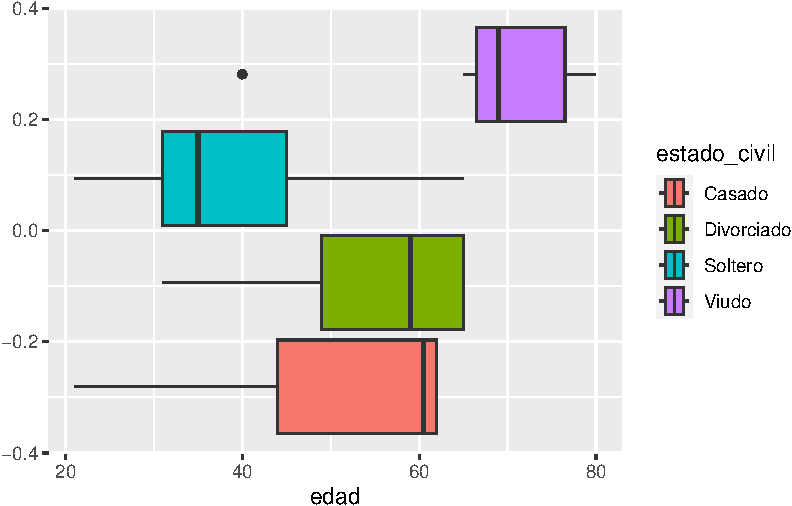
\includegraphics{03-frecuencias-graficos_files/figure-pdf/unnamed-chunk-33-1.pdf}

  \end{tcolorbox}
\item
  Dibujar los histogramas de la edad según el estado civil.

  \begin{tcolorbox}[enhanced jigsaw, toprule=.15mm, rightrule=.15mm, arc=.35mm, colback=white, colbacktitle=quarto-callout-tip-color!10!white, toptitle=1mm, left=2mm, colframe=quarto-callout-tip-color-frame, opacityback=0, breakable, opacitybacktitle=0.6, bottomtitle=1mm, titlerule=0mm, title=\textcolor{quarto-callout-tip-color}{\faLightbulb}\hspace{0.5em}{Solución}, bottomrule=.15mm, coltitle=black, leftrule=.75mm]

\begin{Shaded}
\begin{Highlighting}[]
\FunctionTok{ggplot}\NormalTok{(df, }\FunctionTok{aes}\NormalTok{(}\AttributeTok{x =}\NormalTok{ edad, }\AttributeTok{fill =}\NormalTok{ estado\_civil)) }\SpecialCharTok{+}
    \FunctionTok{geom\_histogram}\NormalTok{(}\AttributeTok{breaks =} \FunctionTok{seq}\NormalTok{(}\DecValTok{20}\NormalTok{, }\DecValTok{80}\NormalTok{, }\DecValTok{10}\NormalTok{), }\AttributeTok{position =} \StringTok{"identity"}\NormalTok{, }\AttributeTok{alpha=}\FloatTok{0.4}\NormalTok{)}
\end{Highlighting}
\end{Shaded}

  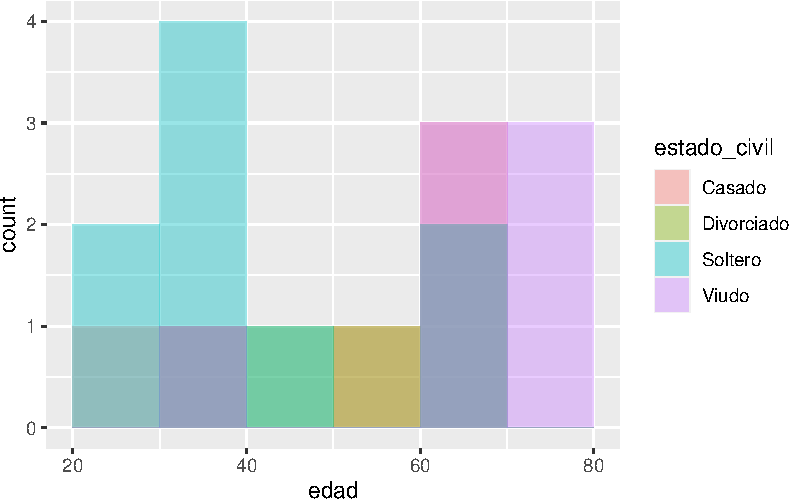
\includegraphics{03-frecuencias-graficos_files/figure-pdf/unnamed-chunk-34-1.pdf}

  Para dibujar cada histograma por separado se puede usar la función
  \href{https://aprendeconalf.es/manual-r/07-graficos.html\#facetas}{\texttt{facet\_wrap}}
  o \texttt{facet\_grid} del paquete \texttt{ggplot2}.

\begin{Shaded}
\begin{Highlighting}[]
\FunctionTok{ggplot}\NormalTok{(df, }\FunctionTok{aes}\NormalTok{(}\AttributeTok{x =}\NormalTok{ edad, }\AttributeTok{fill =}\NormalTok{ estado\_civil)) }\SpecialCharTok{+}
    \FunctionTok{geom\_histogram}\NormalTok{(}\AttributeTok{breaks =} \FunctionTok{seq}\NormalTok{(}\DecValTok{20}\NormalTok{, }\DecValTok{80}\NormalTok{, }\DecValTok{10}\NormalTok{)) }\SpecialCharTok{+}
    \CommentTok{\# Añadir la faceta del estado civil}
    \FunctionTok{facet\_grid}\NormalTok{(}\AttributeTok{rows =} \FunctionTok{vars}\NormalTok{(estado\_civil))}
\end{Highlighting}
\end{Shaded}

  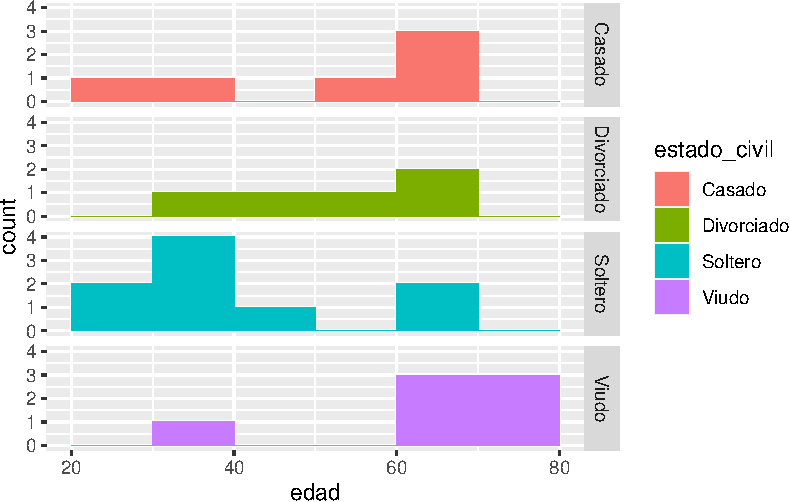
\includegraphics{03-frecuencias-graficos_files/figure-pdf/unnamed-chunk-35-1.pdf}

  \end{tcolorbox}
\end{enumerate}

\end{exercise}

\section{Ejercicios propuestos}\label{ejercicios-propuestos-1}

\begin{exercise}[]\protect\hypertarget{exr-frecuencias-graficos-5}{}\label{exr-frecuencias-graficos-5}

El conjunto de datos \href{datos/neonatos.csv}{neonatos} contiene
información sobre una muestra de 320 recién nacidos en un hospital
durante un año que cumplieron el tiempo normal de gestación.

\begin{enumerate}
\def\labelenumi{\alph{enumi}.}
\item
  Construir la tabla de frecuencias de la puntuación Apgar al minuto de
  nacer. Si se considera que una puntuación Apgar de 3 o menos indica
  que el neonato está deprimido, ¿qué porcentaje de niños está deprimido
  en la muestra?
\item
  Comparar las distribuciones de frecuencias de las puntuaciones Apgar
  al minuto de nacer según si la madre es mayor o menor de 20 años. ¿En
  qué grupo hay más neonatos deprimidos?
\item
  Construir la tabla de frecuencias para el peso de los neonatos,
  agrupando en clases de amplitud \(0.5\) desde el \(2\) hasta el
  \(4.5\). ¿En qué intervalo de peso hay más neonatos?
\item
  Comparar la distribución de frecuencias relativas del peso de los
  neonatos según si la madre fuma o no. Si se considera como peso bajo
  un peso menor de \(2.5\) kg, ¿En qué grupo hay un mayor porcentaje de
  niños con peso bajo?
\item
  Construir el diagrama de barras de la puntuación Apgar al minuto. ¿Qué
  puntuación Apgar es la más frecuente?
\item
  Construir el diagrama de frecuencias relativas acumuladas de la
  puntuación Apgar al minuto. ¿Por debajo de que puntuación estarán la
  mitad de los niños?
\item
  Comparar mediante diagramas de barras de frecuencias relativas las
  distribuciones de las puntuaciones Apgar al minuto según si la madre
  ha fumado o no durante el embarazo. ¿Qué se puede concluir?
\item
  Construir el histograma de pesos, agrupando en clases de amplitud
  \(0.5\) desde el \(2\) hasta el \(4.5\). ¿En qué intervalo de peso hay
  más niños?
\item
  Comparar la distribución de frecuencias relativas del peso de los
  neonatos según si la madre fuma o no. ¿En qué grupo se aprecia menor
  peso de los niños de la muestra?
\item
  Comparar la distribución de frecuencias relativas del peso de los
  neonatos según si la madre fumaba o no antes del embarazo. ¿Qué se
  puede concluir?
\item
  Construir el diagrama de caja y bigotes del peso. ¿Entre qué valores
  se considera que el peso de un neonato es normal? ¿Existen datos
  atípicos?
\item
  Comparar el diagrama de cajas y bigotes del peso, según si la madre
  fumó o no durante el embarazo y si era mayor o no de 20 años. ¿En qué
  grupo el peso tiene más dispersión central? ¿En qué grupo pesan menos
  los niños de la muestra?
\item
  Comparar el diagrama de cajas de la puntuación Apgar al minuto y a los
  cinco minutos. ¿En qué variable hay más dispersión central?
\end{enumerate}

\end{exercise}

\bookmarksetup{startatroot}

\chapter{Estadística Descriptiva}\label{estaduxedstica-descriptiva}

\section{Ejercicios Resueltos}\label{ejercicios-resueltos-2}

Para la realización de esta práctica se requieren los siguientes
paquetes:

\begin{Shaded}
\begin{Highlighting}[]
\FunctionTok{library}\NormalTok{(tidyverse) }
\CommentTok{\# Incluye los siguientes paquetes:}
\CommentTok{\# {-} readr: para la lectura de ficheros csv. }
\CommentTok{\# {-} dplyr: para el preprocesamiento y manipulación de datos.}
\FunctionTok{library}\NormalTok{(vtable) }\CommentTok{\# para resúmenes estadísticos.}
\FunctionTok{library}\NormalTok{(skimr) }\CommentTok{\# para resúmenes estadísticos.}
\FunctionTok{library}\NormalTok{(summarytools) }\CommentTok{\# para resúmenes estadísticos.}
\FunctionTok{library}\NormalTok{(knitr) }\CommentTok{\# para el formateo de tablas.}
\FunctionTok{library}\NormalTok{(kableExtra) }\CommentTok{\# para personalizar el formato de las tablas.}
\end{Highlighting}
\end{Shaded}

\begin{exercise}[]\protect\hypertarget{exr-descriptiva-1}{}\label{exr-descriptiva-1}

En una encuesta a 25 matrimonios sobre el número de hijos que tenían se
obtuvieron los siguientes datos:

\begin{longtable}[]{@{}
  >{\centering\arraybackslash}p{(\columnwidth - 0\tabcolsep) * \real{1.0000}}@{}}
\toprule\noalign{}
\endhead
\bottomrule\noalign{}
\endlastfoot
1, 2, 4, 2, 2, 2, 3, 2, 1, 1, 0, 2, 2, 0, 2, 2, 1, 2, 2, 3, 1, 2, 2, 1,
2 \\
\end{longtable}

\begin{enumerate}
\def\labelenumi{\alph{enumi}.}
\item
  Crear un conjunto de datos con la variable \texttt{hijos}.

  \begin{tcolorbox}[enhanced jigsaw, toprule=.15mm, rightrule=.15mm, arc=.35mm, colback=white, colbacktitle=quarto-callout-tip-color!10!white, toptitle=1mm, left=2mm, colframe=quarto-callout-tip-color-frame, opacityback=0, breakable, opacitybacktitle=0.6, bottomtitle=1mm, titlerule=0mm, title=\textcolor{quarto-callout-tip-color}{\faLightbulb}\hspace{0.5em}{Solución}, bottomrule=.15mm, coltitle=black, leftrule=.75mm]

\begin{Shaded}
\begin{Highlighting}[]
\NormalTok{df }\OtherTok{\textless{}{-}} \FunctionTok{data.frame}\NormalTok{(}\AttributeTok{hijos =} \FunctionTok{c}\NormalTok{(}\DecValTok{1}\NormalTok{, }\DecValTok{2}\NormalTok{, }\DecValTok{4}\NormalTok{, }\DecValTok{2}\NormalTok{, }\DecValTok{2}\NormalTok{, }\DecValTok{2}\NormalTok{, }\DecValTok{3}\NormalTok{, }\DecValTok{2}\NormalTok{, }\DecValTok{1}\NormalTok{, }\DecValTok{1}\NormalTok{, }\DecValTok{0}\NormalTok{, }\DecValTok{2}\NormalTok{, }\DecValTok{2}\NormalTok{, }\DecValTok{0}\NormalTok{, }\DecValTok{2}\NormalTok{, }\DecValTok{2}\NormalTok{, }\DecValTok{1}\NormalTok{, }\DecValTok{2}\NormalTok{, }\DecValTok{2}\NormalTok{, }\DecValTok{3}\NormalTok{, }\DecValTok{1}\NormalTok{, }\DecValTok{2}\NormalTok{, }\DecValTok{2}\NormalTok{, }\DecValTok{1}\NormalTok{, }\DecValTok{2}\NormalTok{))}
\end{Highlighting}
\end{Shaded}

  \end{tcolorbox}
\item
  Calcular el tamaño muestral.

  \begin{tcolorbox}[enhanced jigsaw, toprule=.15mm, rightrule=.15mm, arc=.35mm, colback=white, colbacktitle=quarto-callout-tip-color!10!white, toptitle=1mm, left=2mm, colframe=quarto-callout-tip-color-frame, opacityback=0, breakable, opacitybacktitle=0.6, bottomtitle=1mm, titlerule=0mm, title=\textcolor{quarto-callout-tip-color}{\faLightbulb}\hspace{0.5em}{Solución}, bottomrule=.15mm, coltitle=black, leftrule=.75mm]

\begin{Shaded}
\begin{Highlighting}[]
\FunctionTok{nrow}\NormalTok{(df)}
\end{Highlighting}
\end{Shaded}

\begin{verbatim}
[1] 25
\end{verbatim}

  \end{tcolorbox}
\item
  Calcular la media.

  \begin{tcolorbox}[enhanced jigsaw, toprule=.15mm, rightrule=.15mm, arc=.35mm, colback=white, colbacktitle=quarto-callout-tip-color!10!white, toptitle=1mm, left=2mm, colframe=quarto-callout-tip-color-frame, opacityback=0, breakable, opacitybacktitle=0.6, bottomtitle=1mm, titlerule=0mm, title=\textcolor{quarto-callout-tip-color}{\faLightbulb}\hspace{0.5em}{Solución}, bottomrule=.15mm, coltitle=black, leftrule=.75mm]

\begin{Shaded}
\begin{Highlighting}[]
\FunctionTok{mean}\NormalTok{(df}\SpecialCharTok{$}\NormalTok{hijos)}
\end{Highlighting}
\end{Shaded}

\begin{verbatim}
[1] 1.76
\end{verbatim}

  \end{tcolorbox}
\item
  Calcular la mediana.

  \begin{tcolorbox}[enhanced jigsaw, toprule=.15mm, rightrule=.15mm, arc=.35mm, colback=white, colbacktitle=quarto-callout-tip-color!10!white, toptitle=1mm, left=2mm, colframe=quarto-callout-tip-color-frame, opacityback=0, breakable, opacitybacktitle=0.6, bottomtitle=1mm, titlerule=0mm, title=\textcolor{quarto-callout-tip-color}{\faLightbulb}\hspace{0.5em}{Solución}, bottomrule=.15mm, coltitle=black, leftrule=.75mm]

\begin{Shaded}
\begin{Highlighting}[]
\FunctionTok{median}\NormalTok{(df}\SpecialCharTok{$}\NormalTok{hijos)}
\end{Highlighting}
\end{Shaded}

\begin{verbatim}
[1] 2
\end{verbatim}

  \end{tcolorbox}
\item
  Calcular la moda.

  \begin{tcolorbox}[enhanced jigsaw, toprule=.15mm, rightrule=.15mm, arc=.35mm, colback=white, colbacktitle=quarto-callout-tip-color!10!white, toptitle=1mm, left=2mm, colframe=quarto-callout-tip-color-frame, opacityback=0, breakable, opacitybacktitle=0.6, bottomtitle=1mm, titlerule=0mm, title=\textcolor{quarto-callout-tip-color}{\faLightbulb}\hspace{0.5em}{Solución}, bottomrule=.15mm, coltitle=black, leftrule=.75mm]

  El paquete base de R no tiene implementada ninguna función para
  calcular la moda, así que definiremos nuestra propia función.

\begin{Shaded}
\begin{Highlighting}[]
\NormalTok{moda }\OtherTok{\textless{}{-}} \ControlFlowTok{function}\NormalTok{(x) \{}
\NormalTok{u }\OtherTok{\textless{}{-}} \FunctionTok{unique}\NormalTok{(x) }\CommentTok{\# Vector con los valores de la muestra sin repetir (sin ordenar).}
\NormalTok{tab }\OtherTok{\textless{}{-}} \FunctionTok{tabulate}\NormalTok{(}\FunctionTok{match}\NormalTok{(x, u)) }\CommentTok{\# Frecuencias absolutas de los valores en u.}
\NormalTok{u[tab }\SpecialCharTok{==} \FunctionTok{max}\NormalTok{(tab)] }\CommentTok{\# Valor con la mayor frecuencia.}
\NormalTok{\}}

\FunctionTok{moda}\NormalTok{(df}\SpecialCharTok{$}\NormalTok{hijos)}
\end{Highlighting}
\end{Shaded}

\begin{verbatim}
[1] 2
\end{verbatim}

  \end{tcolorbox}
\item
  Calcular el mínimo.

  \begin{tcolorbox}[enhanced jigsaw, toprule=.15mm, rightrule=.15mm, arc=.35mm, colback=white, colbacktitle=quarto-callout-tip-color!10!white, toptitle=1mm, left=2mm, colframe=quarto-callout-tip-color-frame, opacityback=0, breakable, opacitybacktitle=0.6, bottomtitle=1mm, titlerule=0mm, title=\textcolor{quarto-callout-tip-color}{\faLightbulb}\hspace{0.5em}{Solución}, bottomrule=.15mm, coltitle=black, leftrule=.75mm]

\begin{Shaded}
\begin{Highlighting}[]
\FunctionTok{min}\NormalTok{(df}\SpecialCharTok{$}\NormalTok{hijos)}
\end{Highlighting}
\end{Shaded}

\begin{verbatim}
[1] 0
\end{verbatim}

  \end{tcolorbox}
\item
  Calcular el máximo.

  \begin{tcolorbox}[enhanced jigsaw, toprule=.15mm, rightrule=.15mm, arc=.35mm, colback=white, colbacktitle=quarto-callout-tip-color!10!white, toptitle=1mm, left=2mm, colframe=quarto-callout-tip-color-frame, opacityback=0, breakable, opacitybacktitle=0.6, bottomtitle=1mm, titlerule=0mm, title=\textcolor{quarto-callout-tip-color}{\faLightbulb}\hspace{0.5em}{Solución}, bottomrule=.15mm, coltitle=black, leftrule=.75mm]

\begin{Shaded}
\begin{Highlighting}[]
\FunctionTok{max}\NormalTok{(df}\SpecialCharTok{$}\NormalTok{hijos)}
\end{Highlighting}
\end{Shaded}

\begin{verbatim}
[1] 4
\end{verbatim}

  \end{tcolorbox}
\item
  Calcular los cuartiles.

  \begin{tcolorbox}[enhanced jigsaw, toprule=.15mm, rightrule=.15mm, arc=.35mm, colback=white, colbacktitle=quarto-callout-tip-color!10!white, toptitle=1mm, left=2mm, colframe=quarto-callout-tip-color-frame, opacityback=0, breakable, opacitybacktitle=0.6, bottomtitle=1mm, titlerule=0mm, title=\textcolor{quarto-callout-tip-color}{\faLightbulb}\hspace{0.5em}{Solución}, bottomrule=.15mm, coltitle=black, leftrule=.75mm]

\begin{Shaded}
\begin{Highlighting}[]
\FunctionTok{quantile}\NormalTok{(df}\SpecialCharTok{$}\NormalTok{hijos, }\AttributeTok{prob=}\FunctionTok{c}\NormalTok{(}\FloatTok{0.25}\NormalTok{, }\FloatTok{0.5}\NormalTok{, }\FloatTok{0.75}\NormalTok{))}
\end{Highlighting}
\end{Shaded}

\begin{verbatim}
25% 50% 75% 
  1   2   2 
\end{verbatim}

  \end{tcolorbox}
\item
  Calcular los percentiles 5 y 95.

  \begin{tcolorbox}[enhanced jigsaw, toprule=.15mm, rightrule=.15mm, arc=.35mm, colback=white, colbacktitle=quarto-callout-tip-color!10!white, toptitle=1mm, left=2mm, colframe=quarto-callout-tip-color-frame, opacityback=0, breakable, opacitybacktitle=0.6, bottomtitle=1mm, titlerule=0mm, title=\textcolor{quarto-callout-tip-color}{\faLightbulb}\hspace{0.5em}{Solución}, bottomrule=.15mm, coltitle=black, leftrule=.75mm]

\begin{Shaded}
\begin{Highlighting}[]
\FunctionTok{quantile}\NormalTok{(df}\SpecialCharTok{$}\NormalTok{hijos, }\AttributeTok{prob=}\FunctionTok{c}\NormalTok{(}\FloatTok{0.05}\NormalTok{, }\FloatTok{0.95}\NormalTok{))}
\end{Highlighting}
\end{Shaded}

\begin{verbatim}
 5% 95% 
0.2 3.0 
\end{verbatim}

  \end{tcolorbox}
\item
  Calcular el rango.

  \begin{tcolorbox}[enhanced jigsaw, toprule=.15mm, rightrule=.15mm, arc=.35mm, colback=white, colbacktitle=quarto-callout-tip-color!10!white, toptitle=1mm, left=2mm, colframe=quarto-callout-tip-color-frame, opacityback=0, breakable, opacitybacktitle=0.6, bottomtitle=1mm, titlerule=0mm, title=\textcolor{quarto-callout-tip-color}{\faLightbulb}\hspace{0.5em}{Solución}, bottomrule=.15mm, coltitle=black, leftrule=.75mm]

\begin{Shaded}
\begin{Highlighting}[]
\FunctionTok{max}\NormalTok{(df}\SpecialCharTok{$}\NormalTok{hijos) }\SpecialCharTok{{-}} \FunctionTok{min}\NormalTok{(df}\SpecialCharTok{$}\NormalTok{hijos)}
\end{Highlighting}
\end{Shaded}

\begin{verbatim}
[1] 4
\end{verbatim}

  \end{tcolorbox}
\item
  Calcular el rango intecuartílico.

  \begin{tcolorbox}[enhanced jigsaw, toprule=.15mm, rightrule=.15mm, arc=.35mm, colback=white, colbacktitle=quarto-callout-tip-color!10!white, toptitle=1mm, left=2mm, colframe=quarto-callout-tip-color-frame, opacityback=0, breakable, opacitybacktitle=0.6, bottomtitle=1mm, titlerule=0mm, title=\textcolor{quarto-callout-tip-color}{\faLightbulb}\hspace{0.5em}{Solución}, bottomrule=.15mm, coltitle=black, leftrule=.75mm]

\begin{Shaded}
\begin{Highlighting}[]
\FunctionTok{IQR}\NormalTok{(df}\SpecialCharTok{$}\NormalTok{hijos)}
\end{Highlighting}
\end{Shaded}

\begin{verbatim}
[1] 1
\end{verbatim}

  \end{tcolorbox}
\item
  Calcular la varianza

  \begin{tcolorbox}[enhanced jigsaw, toprule=.15mm, rightrule=.15mm, arc=.35mm, colback=white, colbacktitle=quarto-callout-tip-color!10!white, toptitle=1mm, left=2mm, colframe=quarto-callout-tip-color-frame, opacityback=0, breakable, opacitybacktitle=0.6, bottomtitle=1mm, titlerule=0mm, title=\textcolor{quarto-callout-tip-color}{\faLightbulb}\hspace{0.5em}{Solución}, bottomrule=.15mm, coltitle=black, leftrule=.75mm]

  R dispone de la función \texttt{var} para calcular la
  \emph{cuasivarianza} o \emph{varianza corregida}
  \(\sum \frac{(x_i-\bar x)^2}{n-1}\), pero no dispone de una función
  para calcular la varianza, de manera que para calcularla hay que
  corregir la cuasivarianza.

\begin{Shaded}
\begin{Highlighting}[]
\NormalTok{n }\OtherTok{\textless{}{-}} \FunctionTok{nrow}\NormalTok{(df)}
\CommentTok{\# Cuasivarianza}
\FunctionTok{print}\NormalTok{(}\FunctionTok{paste}\NormalTok{(}\StringTok{"Cuasivarianza:"}\NormalTok{, }\FunctionTok{var}\NormalTok{(df}\SpecialCharTok{$}\NormalTok{hijos)))}
\end{Highlighting}
\end{Shaded}

\begin{verbatim}
[1] "Cuasivarianza: 0.773333333333333"
\end{verbatim}

\begin{Shaded}
\begin{Highlighting}[]
\CommentTok{\# Varianza}
\FunctionTok{print}\NormalTok{(}\FunctionTok{paste}\NormalTok{(}\StringTok{"Varianza: "}\NormalTok{, }\FunctionTok{var}\NormalTok{(df}\SpecialCharTok{$}\NormalTok{hijos)}\SpecialCharTok{*}\NormalTok{(n}\DecValTok{{-}1}\NormalTok{)}\SpecialCharTok{/}\NormalTok{n))}
\end{Highlighting}
\end{Shaded}

\begin{verbatim}
[1] "Varianza:  0.7424"
\end{verbatim}

  \end{tcolorbox}
\item
  Calcular la desviación típica.

  \begin{tcolorbox}[enhanced jigsaw, toprule=.15mm, rightrule=.15mm, arc=.35mm, colback=white, colbacktitle=quarto-callout-tip-color!10!white, toptitle=1mm, left=2mm, colframe=quarto-callout-tip-color-frame, opacityback=0, breakable, opacitybacktitle=0.6, bottomtitle=1mm, titlerule=0mm, title=\textcolor{quarto-callout-tip-color}{\faLightbulb}\hspace{0.5em}{Solución}, bottomrule=.15mm, coltitle=black, leftrule=.75mm]

  R dispone de la función \texttt{sd} para calcular la
  \emph{cuasidesviación típica} o \emph{desviación típica corregida}
  \(\sqrt{\sum \frac{(x_i-\bar x)^2}{n-1}}\), pero no dispone de una
  función para calcular la desviación típica, de manera que para
  calcularla hay que corregir la cuasidesviación típica.

\begin{Shaded}
\begin{Highlighting}[]
\NormalTok{n }\OtherTok{\textless{}{-}} \FunctionTok{nrow}\NormalTok{(df)}
\CommentTok{\# Cuasidesviación típica}
\FunctionTok{print}\NormalTok{(}\FunctionTok{paste}\NormalTok{(}\StringTok{"Cuasidesviación típica:"}\NormalTok{, }\FunctionTok{sd}\NormalTok{(df}\SpecialCharTok{$}\NormalTok{hijos)))}
\end{Highlighting}
\end{Shaded}

\begin{verbatim}
[1] "Cuasidesviación típica: 0.879393730551528"
\end{verbatim}

\begin{Shaded}
\begin{Highlighting}[]
\CommentTok{\# Desviación típica}
\FunctionTok{print}\NormalTok{(}\FunctionTok{paste}\NormalTok{(}\StringTok{"Desviación típica: "}\NormalTok{, }\FunctionTok{sd}\NormalTok{(df}\SpecialCharTok{$}\NormalTok{hijos)}\SpecialCharTok{*}\FunctionTok{sqrt}\NormalTok{((n}\DecValTok{{-}1}\NormalTok{)}\SpecialCharTok{/}\NormalTok{n)))}
\end{Highlighting}
\end{Shaded}

\begin{verbatim}
[1] "Desviación típica:  0.861626369141521"
\end{verbatim}

  \end{tcolorbox}
\item
  Calcular el coeficiente de variación.

  \begin{tcolorbox}[enhanced jigsaw, toprule=.15mm, rightrule=.15mm, arc=.35mm, colback=white, colbacktitle=quarto-callout-tip-color!10!white, toptitle=1mm, left=2mm, colframe=quarto-callout-tip-color-frame, opacityback=0, breakable, opacitybacktitle=0.6, bottomtitle=1mm, titlerule=0mm, title=\textcolor{quarto-callout-tip-color}{\faLightbulb}\hspace{0.5em}{Solución}, bottomrule=.15mm, coltitle=black, leftrule=.75mm]

\begin{Shaded}
\begin{Highlighting}[]
\FunctionTok{sd}\NormalTok{(df}\SpecialCharTok{$}\NormalTok{hijos) }\SpecialCharTok{/} \FunctionTok{abs}\NormalTok{(}\FunctionTok{mean}\NormalTok{(df}\SpecialCharTok{$}\NormalTok{hijos))}
\end{Highlighting}
\end{Shaded}

\begin{verbatim}
[1] 0.4996555
\end{verbatim}

  \end{tcolorbox}
\item
  Calcular el coeficiente de asimetría.

  \begin{tcolorbox}[enhanced jigsaw, toprule=.15mm, rightrule=.15mm, arc=.35mm, colback=white, colbacktitle=quarto-callout-tip-color!10!white, toptitle=1mm, left=2mm, colframe=quarto-callout-tip-color-frame, opacityback=0, breakable, opacitybacktitle=0.6, bottomtitle=1mm, titlerule=0mm, title=\textcolor{quarto-callout-tip-color}{\faLightbulb}\hspace{0.5em}{Solución}, bottomrule=.15mm, coltitle=black, leftrule=.75mm]

  Para calcular el coeficiente de asimetría se utiliza el paquete
  \emph{moments}.

\begin{Shaded}
\begin{Highlighting}[]
\FunctionTok{library}\NormalTok{(moments)}
\FunctionTok{skewness}\NormalTok{(df}\SpecialCharTok{$}\NormalTok{hijos)}
\end{Highlighting}
\end{Shaded}

\begin{verbatim}
[1] 0.1068549
\end{verbatim}

  Como \(g_1\) está próxima a \(0\), la distribución es casi simétrica.

  \end{tcolorbox}
\item
  Calcular el coeficiente de apuntamiento.

  \begin{tcolorbox}[enhanced jigsaw, toprule=.15mm, rightrule=.15mm, arc=.35mm, colback=white, colbacktitle=quarto-callout-tip-color!10!white, toptitle=1mm, left=2mm, colframe=quarto-callout-tip-color-frame, opacityback=0, breakable, opacitybacktitle=0.6, bottomtitle=1mm, titlerule=0mm, title=\textcolor{quarto-callout-tip-color}{\faLightbulb}\hspace{0.5em}{Solución}, bottomrule=.15mm, coltitle=black, leftrule=.75mm]

  Para calcular el coeficiente de apuntamiento se utiliza el paquete
  \emph{moments}.

\begin{Shaded}
\begin{Highlighting}[]
\FunctionTok{library}\NormalTok{(moments)}
\FunctionTok{kurtosis}\NormalTok{(df}\SpecialCharTok{$}\NormalTok{hijos)}
\end{Highlighting}
\end{Shaded}

\begin{verbatim}
[1] 3.71169
\end{verbatim}

  Como \(g_2>0\), la distribución es más apuntada de lo normal
  (leptocúrtica). Como además \(g_2\not\in(-2,2)\) se puede concluir que
  la muestra es demasiado apuntada para provenir de una población
  normal.

  \end{tcolorbox}
\end{enumerate}

\end{exercise}

\begin{exercise}[]\protect\hypertarget{exr-descriptiva-2}{}\label{exr-descriptiva-2}

El fichero \href{datos/colesterol.csv}{\texttt{colesterol.csv}} contiene
información de una muestra de pacientes donde se han medido la edad, el
sexo, el peso, la altura y el nivel de colesterol, además de su nombre.

\begin{enumerate}
\def\labelenumi{\alph{enumi}.}
\item
  Crear un data frame con los datos de todos los pacientes del estudio a
  partir del fichero
  \href{datos/colesterol.csv}{\texttt{colesterol.csv}}.

  \begin{tcolorbox}[enhanced jigsaw, toprule=.15mm, rightrule=.15mm, arc=.35mm, colback=white, colbacktitle=quarto-callout-tip-color!10!white, toptitle=1mm, left=2mm, colframe=quarto-callout-tip-color-frame, opacityback=0, breakable, opacitybacktitle=0.6, bottomtitle=1mm, titlerule=0mm, title=\textcolor{quarto-callout-tip-color}{\faLightbulb}\hspace{0.5em}{Solución}, bottomrule=.15mm, coltitle=black, leftrule=.75mm]

\begin{Shaded}
\begin{Highlighting}[]
\NormalTok{df }\OtherTok{\textless{}{-}} \FunctionTok{read.csv}\NormalTok{(}\StringTok{"https://raw.githubusercontent.com/asalber/estadistica{-}practicas{-}r/main/datos/colesterol.csv"}\NormalTok{)}
\NormalTok{df}
\end{Highlighting}
\end{Shaded}

\begin{verbatim}
                            nombre edad sexo peso altura colesterol
1     José Luis Martínez Izquierdo   18    H   85   1.79        182
2                   Rosa Díaz Díaz   32    M   65   1.73        232
3            Javier García Sánchez   24    H   NA   1.81        191
4              Carmen López Pinzón   35    M   65   1.70        200
5             Marisa López Collado   46    M   51   1.58        148
6                Antonio Ruiz Cruz   68    H   66   1.74        249
7          Antonio Fernández Ocaña   51    H   62   1.72        276
8            Pilar Martín González   22    M   60   1.66         NA
9             Pedro Gálvez Tenorio   35    H   90   1.94        241
10         Santiago Reillo Manzano   46    H   75   1.85        280
11           Macarena Álvarez Luna   53    M   55   1.62        262
12      José María de la Guía Sanz   58    H   78   1.87        198
13 Miguel Angel Cuadrado Gutiérrez   27    H  109   1.98        210
14           Carolina Rubio Moreno   20    M   61   1.77        194
\end{verbatim}

  \end{tcolorbox}
\item
  Calcular el tamaño muestral según el sexo.

  \begin{tcolorbox}[enhanced jigsaw, toprule=.15mm, rightrule=.15mm, arc=.35mm, colback=white, colbacktitle=quarto-callout-tip-color!10!white, toptitle=1mm, left=2mm, colframe=quarto-callout-tip-color-frame, opacityback=0, breakable, opacitybacktitle=0.6, bottomtitle=1mm, titlerule=0mm, title=\textcolor{quarto-callout-tip-color}{\faLightbulb}\hspace{0.5em}{Solución 1}, bottomrule=.15mm, coltitle=black, leftrule=.75mm]

\begin{Shaded}
\begin{Highlighting}[]
\FunctionTok{table}\NormalTok{(df}\SpecialCharTok{$}\NormalTok{sexo)}
\end{Highlighting}
\end{Shaded}

\begin{verbatim}

H M 
8 6 
\end{verbatim}

  \end{tcolorbox}

  \begin{tcolorbox}[enhanced jigsaw, toprule=.15mm, rightrule=.15mm, arc=.35mm, colback=white, colbacktitle=quarto-callout-tip-color!10!white, toptitle=1mm, left=2mm, colframe=quarto-callout-tip-color-frame, opacityback=0, breakable, opacitybacktitle=0.6, bottomtitle=1mm, titlerule=0mm, title=\textcolor{quarto-callout-tip-color}{\faLightbulb}\hspace{0.5em}{Solución 2}, bottomrule=.15mm, coltitle=black, leftrule=.75mm]

\begin{Shaded}
\begin{Highlighting}[]
\FunctionTok{library}\NormalTok{(dplyr)}
\FunctionTok{count}\NormalTok{(df, sexo)}
\end{Highlighting}
\end{Shaded}

\begin{verbatim}
  sexo n
1    H 8
2    M 6
\end{verbatim}

  \end{tcolorbox}
\item
  Calcular la media y la desviación típica del nivel de colesterol sin
  tener en cuenta los datos perdidos.

  \begin{tcolorbox}[enhanced jigsaw, toprule=.15mm, rightrule=.15mm, arc=.35mm, colback=white, colbacktitle=quarto-callout-tip-color!10!white, toptitle=1mm, left=2mm, colframe=quarto-callout-tip-color-frame, opacityback=0, breakable, opacitybacktitle=0.6, bottomtitle=1mm, titlerule=0mm, title=\textcolor{quarto-callout-tip-color}{\faLightbulb}\hspace{0.5em}{Solución}, bottomrule=.15mm, coltitle=black, leftrule=.75mm]

\begin{Shaded}
\begin{Highlighting}[]
\FunctionTok{print}\NormalTok{(}\FunctionTok{paste}\NormalTok{(}\StringTok{"Media:"}\NormalTok{, }\FunctionTok{mean}\NormalTok{(df}\SpecialCharTok{$}\NormalTok{colesterol, }\AttributeTok{na.rm =} \ConstantTok{TRUE}\NormalTok{)))}
\end{Highlighting}
\end{Shaded}

\begin{verbatim}
[1] "Media: 220.230769230769"
\end{verbatim}

\begin{Shaded}
\begin{Highlighting}[]
\FunctionTok{print}\NormalTok{(}\FunctionTok{paste}\NormalTok{(}\StringTok{"Desviación típica:"}\NormalTok{, }\FunctionTok{sd}\NormalTok{(df}\SpecialCharTok{$}\NormalTok{colesterol, }\AttributeTok{na.rm =} \ConstantTok{TRUE}\NormalTok{)))}
\end{Highlighting}
\end{Shaded}

\begin{verbatim}
[1] "Desviación típica: 39.8479481825473"
\end{verbatim}

  \end{tcolorbox}
\item
  Realizar un resumen estadístico con la media, el mínimo, los cuartiles
  y el máximo.

  \begin{tcolorbox}[enhanced jigsaw, toprule=.15mm, rightrule=.15mm, arc=.35mm, colback=white, colbacktitle=quarto-callout-tip-color!10!white, toptitle=1mm, left=2mm, colframe=quarto-callout-tip-color-frame, opacityback=0, breakable, opacitybacktitle=0.6, bottomtitle=1mm, titlerule=0mm, title=\textcolor{quarto-callout-tip-color}{\faLightbulb}\hspace{0.5em}{Solución 1}, bottomrule=.15mm, coltitle=black, leftrule=.75mm]

  Usando el paquete base de R.

\begin{Shaded}
\begin{Highlighting}[]
\FunctionTok{summary}\NormalTok{(df)}
\end{Highlighting}
\end{Shaded}

\begin{verbatim}
    nombre               edad           sexo                peso       
 Length:14          Min.   :18.00   Length:14          Min.   : 51.00  
 Class :character   1st Qu.:24.75   Class :character   1st Qu.: 61.00  
 Mode  :character   Median :35.00   Mode  :character   Median : 65.00  
                    Mean   :38.21                      Mean   : 70.92  
                    3rd Qu.:49.75                      3rd Qu.: 78.00  
                    Max.   :68.00                      Max.   :109.00  
                                                       NA's   :1       
     altura        colesterol   
 Min.   :1.580   Min.   :148.0  
 1st Qu.:1.705   1st Qu.:194.0  
 Median :1.755   Median :210.0  
 Mean   :1.769   Mean   :220.2  
 3rd Qu.:1.840   3rd Qu.:249.0  
 Max.   :1.980   Max.   :280.0  
                 NA's   :1      
\end{verbatim}

  \end{tcolorbox}

  \begin{tcolorbox}[enhanced jigsaw, toprule=.15mm, rightrule=.15mm, arc=.35mm, colback=white, colbacktitle=quarto-callout-tip-color!10!white, toptitle=1mm, left=2mm, colframe=quarto-callout-tip-color-frame, opacityback=0, breakable, opacitybacktitle=0.6, bottomtitle=1mm, titlerule=0mm, title=\textcolor{quarto-callout-tip-color}{\faLightbulb}\hspace{0.5em}{Solución 2}, bottomrule=.15mm, coltitle=black, leftrule=.75mm]

  Usando la función \texttt{st} del paquete
  \href{https://cran.r-project.org/web/packages/vtable/vignettes/sumtable.html}{\texttt{vtable}}.

\begin{Shaded}
\begin{Highlighting}[]
\FunctionTok{library}\NormalTok{(vtable)}
\FunctionTok{st}\NormalTok{(df)}
\end{Highlighting}
\end{Shaded}

  \begin{table}

  \caption{\label{tab:unnamed-chunk-22}Summary Statistics}
  \centering
  \begin{tabular}[t]{llllllll}
  \toprule
  Variable & N & Mean & Std. Dev. & Min & Pctl. 25 & Pctl. 75 & Max\\
  \midrule
  edad & 14 & 38 & 16 & 18 & 25 & 50 & 68\\
  sexo & 14 &  &  &  &  &  & \\
  ... H & 8 & 57\% &  &  &  &  & \\
  ... M & 6 & 43\% &  &  &  &  & \\
  peso & 13 & 71 & 16 & 51 & 61 & 78 & 109\\
  \addlinespace
  altura & 14 & 1.8 & 0.12 & 1.6 & 1.7 & 1.8 & 2\\
  colesterol & 13 & 220 & 40 & 148 & 194 & 249 & 280\\
  \bottomrule
  \end{tabular}
  \end{table}

  \end{tcolorbox}

  \begin{tcolorbox}[enhanced jigsaw, toprule=.15mm, rightrule=.15mm, arc=.35mm, colback=white, colbacktitle=quarto-callout-tip-color!10!white, toptitle=1mm, left=2mm, colframe=quarto-callout-tip-color-frame, opacityback=0, breakable, opacitybacktitle=0.6, bottomtitle=1mm, titlerule=0mm, title=\textcolor{quarto-callout-tip-color}{\faLightbulb}\hspace{0.5em}{Solución 3}, bottomrule=.15mm, coltitle=black, leftrule=.75mm]

  Usando la función \texttt{skim} del paquete
  \href{https://cran.r-project.org/web/packages/skimr/vignettes/skimr.html}{\texttt{skimr}}.

\begin{Shaded}
\begin{Highlighting}[]
\FunctionTok{library}\NormalTok{(skimr)}
\FunctionTok{skim}\NormalTok{(df)}
\end{Highlighting}
\end{Shaded}

  \begin{table}

  \caption{\label{tab:unnamed-chunk-23}Data summary}
  \centering
  \begin{tabular}[t]{l|l}
  \hline
  Name & df\\
  \hline
  Number of rows & 14\\
  \hline
  Number of columns & 6\\
  \hline
  \_\_\_\_\_\_\_\_\_\_\_\_\_\_\_\_\_\_\_\_\_\_\_ & \\
  \hline
  Column type frequency: & \\
  \hline
  character & 2\\
  \hline
  numeric & 4\\
  \hline
  \_\_\_\_\_\_\_\_\_\_\_\_\_\_\_\_\_\_\_\_\_\_\_\_ & \\
  \hline
  Group variables & None\\
  \hline
  \end{tabular}
  \end{table}

  \textbf{Variable type: character}

  \begin{tabular}{l|r|r|r|r|r|r|r}
  \hline
  skim\_variable & n\_missing & complete\_rate & min & max & empty & n\_unique & whitespace\\
  \hline
  nombre & 0 & 1 & 14 & 31 & 0 & 14 & 0\\
  \hline
  sexo & 0 & 1 & 1 & 1 & 0 & 2 & 0\\
  \hline
  \end{tabular}

  \textbf{Variable type: numeric}

  \begin{tabular}{l|r|r|r|r|r|r|r|r|r|l}
  \hline
  skim\_variable & n\_missing & complete\_rate & mean & sd & p0 & p25 & p50 & p75 & p100 & hist\\
  \hline
  edad & 0 & 1.00 & 38.21 & 15.62 & 18.00 & 24.75 & 35.00 & 49.75 & 68.00 & ▇▅▃▅▂\\
  \hline
  peso & 1 & 0.93 & 70.92 & 16.13 & 51.00 & 61.00 & 65.00 & 78.00 & 109.00 & ▇▅▅▂▂\\
  \hline
  altura & 0 & 1.00 & 1.77 & 0.12 & 1.58 & 1.70 & 1.75 & 1.84 & 1.98 & ▆▇▆▃▃\\
  \hline
  colesterol & 1 & 0.93 & 220.23 & 39.85 & 148.00 & 194.00 & 210.00 & 249.00 & 280.00 & ▂▇▂▅▅\\
  \hline
  \end{tabular}

  \end{tcolorbox}

  \begin{tcolorbox}[enhanced jigsaw, toprule=.15mm, rightrule=.15mm, arc=.35mm, colback=white, colbacktitle=quarto-callout-tip-color!10!white, toptitle=1mm, left=2mm, colframe=quarto-callout-tip-color-frame, opacityback=0, breakable, opacitybacktitle=0.6, bottomtitle=1mm, titlerule=0mm, title=\textcolor{quarto-callout-tip-color}{\faLightbulb}\hspace{0.5em}{Solución 4}, bottomrule=.15mm, coltitle=black, leftrule=.75mm]

  Usando las funciones \texttt{descr} y \texttt{dfSummary} del paquete
  \href{https://cran.r-project.org/web/packages/summarytools/vignettes/introduction.html}{\texttt{summarytools}}.

\begin{Shaded}
\begin{Highlighting}[]
\FunctionTok{library}\NormalTok{(summarytools)}
\FunctionTok{descr}\NormalTok{(df) }\SpecialCharTok{|\textgreater{}}
\FunctionTok{kable}\NormalTok{() }\SpecialCharTok{|\textgreater{}}
\FunctionTok{kable\_styling}\NormalTok{()}
\end{Highlighting}
\end{Shaded}

  \begin{table}
  \centering
  \begin{tabular}{l|r|r|r|r}
  \hline
    & altura & colesterol & edad & peso\\
  \hline
  Mean & 1.7685714 & 220.2307692 & 38.2142857 & 70.9230769\\
  \hline
  Std.Dev & 0.1150155 & 39.8479482 & 15.6213787 & 16.1269006\\
  \hline
  Min & 1.5800000 & 148.0000000 & 18.0000000 & 51.0000000\\
  \hline
  Q1 & 1.7000000 & 194.0000000 & 24.0000000 & 61.0000000\\
  \hline
  Median & 1.7550000 & 210.0000000 & 35.0000000 & 65.0000000\\
  \hline
  Q3 & 1.8500000 & 249.0000000 & 51.0000000 & 78.0000000\\
  \hline
  Max & 1.9800000 & 280.0000000 & 68.0000000 & 109.0000000\\
  \hline
  MAD & 0.1111950 & 41.5128000 & 17.7912000 & 14.8260000\\
  \hline
  IQR & 0.1350000 & 55.0000000 & 25.0000000 & 17.0000000\\
  \hline
  CV & 0.0650330 & 0.1809372 & 0.4087837 & 0.2273858\\
  \hline
  Skewness & 0.2052057 & -0.0022401 & 0.3238511 & 0.9149779\\
  \hline
  SE.Skewness & 0.5973799 & 0.6163361 & 0.5973799 & 0.6163361\\
  \hline
  Kurtosis & -0.9852205 & -1.2502343 & -1.2886761 & -0.1208155\\
  \hline
  N.Valid & 14.0000000 & 13.0000000 & 14.0000000 & 13.0000000\\
  \hline
  Pct.Valid & 100.0000000 & 92.8571429 & 100.0000000 & 92.8571429\\
  \hline
  \end{tabular}
  \end{table}

\begin{Shaded}
\begin{Highlighting}[]
\FunctionTok{print}\NormalTok{(}\FunctionTok{dfSummary}\NormalTok{(df, }\AttributeTok{plain.ascii =} \ConstantTok{FALSE}\NormalTok{, }\AttributeTok{style =} \StringTok{"grid"}\NormalTok{), }\AttributeTok{method =} \StringTok{"render"}\NormalTok{)}
\end{Highlighting}
\end{Shaded}

  \begin{longtable}[]{@{}
    >{\centering\arraybackslash}p{(\columnwidth - 12\tabcolsep) * \real{0.1429}}
    >{\raggedright\arraybackslash}p{(\columnwidth - 12\tabcolsep) * \real{0.1429}}
    >{\raggedright\arraybackslash}p{(\columnwidth - 12\tabcolsep) * \real{0.1429}}
    >{\raggedright\arraybackslash}p{(\columnwidth - 12\tabcolsep) * \real{0.1429}}
    >{\raggedright\arraybackslash}p{(\columnwidth - 12\tabcolsep) * \real{0.1429}}
    >{\centering\arraybackslash}p{(\columnwidth - 12\tabcolsep) * \real{0.1429}}
    >{\centering\arraybackslash}p{(\columnwidth - 12\tabcolsep) * \real{0.1429}}@{}}
  \toprule\noalign{}
  \begin{minipage}[b]{\linewidth}\centering
  \textbf{No}
  \end{minipage} & \begin{minipage}[b]{\linewidth}\centering
  \textbf{Variable}
  \end{minipage} & \begin{minipage}[b]{\linewidth}\centering
  \textbf{Stats / Values}
  \end{minipage} & \begin{minipage}[b]{\linewidth}\centering
  \textbf{Freqs (\% of Valid)}
  \end{minipage} & \begin{minipage}[b]{\linewidth}\centering
  \textbf{Graph}
  \end{minipage} & \begin{minipage}[b]{\linewidth}\centering
  \textbf{Valid}
  \end{minipage} & \begin{minipage}[b]{\linewidth}\centering
  \textbf{Missing}
  \end{minipage} \\
  \midrule\noalign{}
  \endhead
  \bottomrule\noalign{}
  \endlastfoot
  1 & nombre {[}character{]} &
  \begin{minipage}[t]{\linewidth}\raggedright
  \begin{longtable}[]{@{}l@{}}
  \toprule\noalign{}
  \endhead
  \bottomrule\noalign{}
  \endlastfoot
  1. Antonio Fernández Ocaña \\
  2. Antonio Ruiz Cruz \\
  3. Carmen López Pinzón \\
  4. Carolina Rubio Moreno \\
  5. Javier García Sánchez \\
  6. José Luis Martínez Izquie \\
  7. José María de la Guía San \\
  8. Macarena Álvarez Luna \\
  9. Marisa López Collado \\
  10. Miguel Angel Cuadrado Gut \\
  {[} 4 others {]} \\
  \end{longtable}
  \end{minipage} & \begin{minipage}[t]{\linewidth}\raggedright
  \begin{longtable}[]{@{}rlrl@{}}
  \toprule\noalign{}
  \endhead
  \bottomrule\noalign{}
  \endlastfoot
  1 & ( & 7.1\% & ) \\
  1 & ( & 7.1\% & ) \\
  1 & ( & 7.1\% & ) \\
  1 & ( & 7.1\% & ) \\
  1 & ( & 7.1\% & ) \\
  1 & ( & 7.1\% & ) \\
  1 & ( & 7.1\% & ) \\
  1 & ( & 7.1\% & ) \\
  1 & ( & 7.1\% & ) \\
  1 & ( & 7.1\% & ) \\
  4 & ( & 28.6\% & ) \\
  \end{longtable}
  \end{minipage} & & 14 (100.0\%) & 0 (0.0\%) \\
  2 & edad {[}integer{]} & \begin{minipage}[t]{\linewidth}\raggedright
  \begin{longtable}[]{@{}l@{}}
  \toprule\noalign{}
  \endhead
  \bottomrule\noalign{}
  \endlastfoot
  Mean (sd) : 38.2 (15.6) \\
  min ≤ med ≤ max: \\
  18 ≤ 35 ≤ 68 \\
  IQR (CV) : 25 (0.4) \\
  \end{longtable}
  \end{minipage} & 12 distinct values & & 14 (100.0\%) & 0 (0.0\%) \\
  3 & sexo {[}character{]} & \begin{minipage}[t]{\linewidth}\raggedright
  \begin{longtable}[]{@{}l@{}}
  \toprule\noalign{}
  \endhead
  \bottomrule\noalign{}
  \endlastfoot
  1. H \\
  2. M \\
  \end{longtable}
  \end{minipage} & \begin{minipage}[t]{\linewidth}\raggedright
  \begin{longtable}[]{@{}rlrl@{}}
  \toprule\noalign{}
  \endhead
  \bottomrule\noalign{}
  \endlastfoot
  8 & ( & 57.1\% & ) \\
  6 & ( & 42.9\% & ) \\
  \end{longtable}
  \end{minipage} & & 14 (100.0\%) & 0 (0.0\%) \\
  4 & peso {[}numeric{]} & \begin{minipage}[t]{\linewidth}\raggedright
  \begin{longtable}[]{@{}l@{}}
  \toprule\noalign{}
  \endhead
  \bottomrule\noalign{}
  \endlastfoot
  Mean (sd) : 70.9 (16.1) \\
  min ≤ med ≤ max: \\
  51 ≤ 65 ≤ 109 \\
  IQR (CV) : 17 (0.2) \\
  \end{longtable}
  \end{minipage} & 12 distinct values & & 13 (92.9\%) & 1 (7.1\%) \\
  5 & altura {[}numeric{]} & \begin{minipage}[t]{\linewidth}\raggedright
  \begin{longtable}[]{@{}l@{}}
  \toprule\noalign{}
  \endhead
  \bottomrule\noalign{}
  \endlastfoot
  Mean (sd) : 1.8 (0.1) \\
  min ≤ med ≤ max: \\
  1.6 ≤ 1.8 ≤ 2 \\
  IQR (CV) : 0.1 (0.1) \\
  \end{longtable}
  \end{minipage} & 14 distinct values & & 14 (100.0\%) & 0 (0.0\%) \\
  6 & colesterol {[}numeric{]} &
  \begin{minipage}[t]{\linewidth}\raggedright
  \begin{longtable}[]{@{}l@{}}
  \toprule\noalign{}
  \endhead
  \bottomrule\noalign{}
  \endlastfoot
  Mean (sd) : 220.2 (39.8) \\
  min ≤ med ≤ max: \\
  148 ≤ 210 ≤ 280 \\
  IQR (CV) : 55 (0.2) \\
  \end{longtable}
  \end{minipage} & 13 distinct values & & 13 (92.9\%) & 1 (7.1\%) \\
  \end{longtable}

  \end{tcolorbox}
\item
  ¿En qué variable es más representativa la media?

  \begin{tcolorbox}[enhanced jigsaw, toprule=.15mm, rightrule=.15mm, arc=.35mm, colback=white, colbacktitle=quarto-callout-tip-color!10!white, toptitle=1mm, left=2mm, colframe=quarto-callout-tip-color-frame, opacityback=0, breakable, opacitybacktitle=0.6, bottomtitle=1mm, titlerule=0mm, title=\textcolor{quarto-callout-tip-color}{\faLightbulb}\hspace{0.5em}{Solución 1}, bottomrule=.15mm, coltitle=black, leftrule=.75mm]

  Usando la función \texttt{sumtable} del paquete
  \href{https://cran.r-project.org/web/packages/vtable/vignettes/sumtable.html}{\texttt{vtable}}.

\begin{Shaded}
\begin{Highlighting}[]
\FunctionTok{library}\NormalTok{(vtable)}
\FunctionTok{sumtable}\NormalTok{(df, }\AttributeTok{summ =} \FunctionTok{c}\NormalTok{(}\StringTok{\textquotesingle{}mean(x)\textquotesingle{}}\NormalTok{, }\StringTok{\textquotesingle{}sd(x)\textquotesingle{}}\NormalTok{, }\StringTok{\textquotesingle{}sd(x)/mean(x)\textquotesingle{}}\NormalTok{),}
\AttributeTok{summ.names =} \FunctionTok{c}\NormalTok{(}\StringTok{"Media"}\NormalTok{, }\StringTok{"Desviación Típica"}\NormalTok{, }\StringTok{"Coef. Variación"}\NormalTok{))}
\end{Highlighting}
\end{Shaded}

  \begin{table}

  \caption{\label{tab:unnamed-chunk-25}Summary Statistics}
  \centering
  \begin{tabular}[t]{llll}
  \toprule
  Variable & Media & Desviación Típica & Coef. Variación\\
  \midrule
  edad & 38 & 16 & 0.41\\
  sexo & 14 &  & \\
  ... H & 8 & 57\% & \\
  ... M & 6 & 43\% & \\
  peso & 71 & 16 & 0.23\\
  \addlinespace
  altura & 1.8 & 0.12 & 0.065\\
  colesterol & 220 & 40 & 0.18\\
  \bottomrule
  \end{tabular}
  \end{table}

  La variable con el coeficiente de variación más pequeño es la altura,
  por lo que es la que tiene la media más representativa.

  \end{tcolorbox}

  \begin{tcolorbox}[enhanced jigsaw, toprule=.15mm, rightrule=.15mm, arc=.35mm, colback=white, colbacktitle=quarto-callout-tip-color!10!white, toptitle=1mm, left=2mm, colframe=quarto-callout-tip-color-frame, opacityback=0, breakable, opacitybacktitle=0.6, bottomtitle=1mm, titlerule=0mm, title=\textcolor{quarto-callout-tip-color}{\faLightbulb}\hspace{0.5em}{Solución 2}, bottomrule=.15mm, coltitle=black, leftrule=.75mm]

  Usando las funciones \texttt{summarise} y \texttt{across} del paquete
  \texttt{dplyr}.

\begin{Shaded}
\begin{Highlighting}[]
\FunctionTok{library}\NormalTok{(dplyr)}
\FunctionTok{summarise}\NormalTok{(df, }\FunctionTok{across}\NormalTok{(}\AttributeTok{.cols =} \FunctionTok{where}\NormalTok{(is.numeric), }\AttributeTok{.fns =} \FunctionTok{list}\NormalTok{(}\AttributeTok{Media =} \SpecialCharTok{\textasciitilde{}} \FunctionTok{mean}\NormalTok{(.x, }\AttributeTok{na.rm =}\NormalTok{ T), }\StringTok{\textasciigrave{}}\AttributeTok{Desviación Típica}\StringTok{\textasciigrave{}} \OtherTok{=} \ErrorTok{\textasciitilde{}} \FunctionTok{sd}\NormalTok{(.x, }\AttributeTok{na.rm =}\NormalTok{ T), }\StringTok{\textasciigrave{}}\AttributeTok{Coef. Variación}\StringTok{\textasciigrave{}} \OtherTok{=} \ErrorTok{\textasciitilde{}} \FunctionTok{sd}\NormalTok{(.x, }\AttributeTok{na.rm=}\NormalTok{T) }\SpecialCharTok{/} \FunctionTok{mean}\NormalTok{(.x, }\AttributeTok{na.rm=}\NormalTok{T)))) }\SpecialCharTok{|\textgreater{}}
\FunctionTok{kable}\NormalTok{() }\SpecialCharTok{|\textgreater{}}
\FunctionTok{kable\_styling}\NormalTok{()}
\end{Highlighting}
\end{Shaded}

  \begin{table}
  \centering
  \begin{tabular}{r|r|r|r|r|r|r|r|r|r|r|r}
  \hline
  edad\_Media & edad\_Desviación Típica & edad\_Coef. Variación & peso\_Media & peso\_Desviación Típica & peso\_Coef. Variación & altura\_Media & altura\_Desviación Típica & altura\_Coef. Variación & colesterol\_Media & colesterol\_Desviación Típica & colesterol\_Coef. Variación\\
  \hline
  38.21429 & 15.62138 & 0.4087837 & 70.92308 & 16.1269 & 0.2273858 & 1.768571 & 0.1150155 & 0.065033 & 220.2308 & 39.84795 & 0.1809372\\
  \hline
  \end{tabular}
  \end{table}

  \end{tcolorbox}

  \begin{tcolorbox}[enhanced jigsaw, toprule=.15mm, rightrule=.15mm, arc=.35mm, colback=white, colbacktitle=quarto-callout-tip-color!10!white, toptitle=1mm, left=2mm, colframe=quarto-callout-tip-color-frame, opacityback=0, breakable, opacitybacktitle=0.6, bottomtitle=1mm, titlerule=0mm, title=\textcolor{quarto-callout-tip-color}{\faLightbulb}\hspace{0.5em}{Solución 3}, bottomrule=.15mm, coltitle=black, leftrule=.75mm]

  Usando las funciones \texttt{group\_by} y \texttt{summarise} del
  paquete \texttt{dplyr} y pivotando el data frame a formato largo.

\begin{Shaded}
\begin{Highlighting}[]
\FunctionTok{library}\NormalTok{(tidyverse)}
\NormalTok{df }\SpecialCharTok{|\textgreater{}} \FunctionTok{select}\NormalTok{(}\FunctionTok{where}\NormalTok{(is.numeric)) }\SpecialCharTok{|\textgreater{}} 
    \FunctionTok{pivot\_longer}\NormalTok{(}\FunctionTok{everything}\NormalTok{(), }\AttributeTok{names\_to =} \StringTok{"Variable"}\NormalTok{, }\AttributeTok{values\_to =} \StringTok{"Valor"}\NormalTok{) }\SpecialCharTok{|\textgreater{}}
    \FunctionTok{group\_by}\NormalTok{(Variable) }\SpecialCharTok{|\textgreater{}}
    \FunctionTok{summarise}\NormalTok{(}\StringTok{"Media"} \OtherTok{=} \FunctionTok{mean}\NormalTok{(Valor, }\AttributeTok{na.rm =}\NormalTok{ T), }
    \StringTok{"Desviación Típica"} \OtherTok{=} \FunctionTok{sd}\NormalTok{(Valor, }\AttributeTok{na.rm =}\NormalTok{ T),}
    \StringTok{"Coef. Variación"} \OtherTok{=} \FunctionTok{sd}\NormalTok{(Valor, }\AttributeTok{na.rm =}\NormalTok{ T) }\SpecialCharTok{/} \FunctionTok{mean}\NormalTok{(Valor, }\AttributeTok{na.rm =}\NormalTok{ T)) }\SpecialCharTok{|\textgreater{}}
    \FunctionTok{kable}\NormalTok{() }\SpecialCharTok{|\textgreater{}}
    \FunctionTok{kable\_styling}\NormalTok{()}
\end{Highlighting}
\end{Shaded}

  \begin{table}
  \centering
  \begin{tabular}{l|r|r|r}
  \hline
  Variable & Media & Desviación Típica & Coef. Variación\\
  \hline
  altura & 1.768571 & 0.1150155 & 0.0650330\\
  \hline
  colesterol & 220.230769 & 39.8479482 & 0.1809372\\
  \hline
  edad & 38.214286 & 15.6213787 & 0.4087837\\
  \hline
  peso & 70.923077 & 16.1269006 & 0.2273858\\
  \hline
  \end{tabular}
  \end{table}

  La variable con el coeficiente de variación más pequeño es la altura,
  por lo que es la que tiene la media más representativa.

  \end{tcolorbox}
\item
  Realizar un resumen estadístico con el coeficiente de asimetría y el
  coeficiente de apuntamiento del peso y la estatura según el sexo. ¿Qué
  grupo tiene peso más normal, los hombres o las mujeres? ¿Y una
  estatura más normal?

  \begin{tcolorbox}[enhanced jigsaw, toprule=.15mm, rightrule=.15mm, arc=.35mm, colback=white, colbacktitle=quarto-callout-tip-color!10!white, toptitle=1mm, left=2mm, colframe=quarto-callout-tip-color-frame, opacityback=0, breakable, opacitybacktitle=0.6, bottomtitle=1mm, titlerule=0mm, title=\textcolor{quarto-callout-tip-color}{\faLightbulb}\hspace{0.5em}{Solución 1}, bottomrule=.15mm, coltitle=black, leftrule=.75mm]

  Usando la función \texttt{sumtable} del paquete
  \href{https://cran.r-project.org/web/packages/vtable/vignettes/sumtable.html}{\texttt{vtable}}.

\begin{Shaded}
\begin{Highlighting}[]
\FunctionTok{library}\NormalTok{(vtable)}
\FunctionTok{sumtable}\NormalTok{(df, }\AttributeTok{vars =} \FunctionTok{c}\NormalTok{(}\StringTok{"peso"}\NormalTok{, }\StringTok{"altura"}\NormalTok{), }\AttributeTok{group =} \StringTok{"sexo"}\NormalTok{, }\AttributeTok{summ =} \FunctionTok{c}\NormalTok{(}\StringTok{\textquotesingle{}skewness(x)\textquotesingle{}}\NormalTok{, }\StringTok{\textquotesingle{}kurtosis(x)\textquotesingle{}}\NormalTok{),}
\AttributeTok{summ.names =} \FunctionTok{c}\NormalTok{(}\StringTok{"Coef. Asimetría"}\NormalTok{, }\StringTok{"Coef. Apuntamiento"}\NormalTok{))}
\end{Highlighting}
\end{Shaded}

  \begin{table}

  \caption{\label{tab:unnamed-chunk-28}Summary Statistics}
  \centering
  \begin{tabular}[t]{lllll}
  \toprule
  \multicolumn{1}{c}{sexo} & \multicolumn{2}{c}{H} & \multicolumn{2}{c}{M} \\
  \cmidrule(l{3pt}r{3pt}){1-1} \cmidrule(l{3pt}r{3pt}){2-3} \cmidrule(l{3pt}r{3pt}){4-5}
  Variable & Coef. Asimetría & Coef. Apuntamiento & Coef. Asimetría & Coef. Apuntamiento\\
  \midrule
  peso & 0.61 & 2.5 & -0.47 & 1.9\\
  altura & 0.27 & 1.9 & -0.07 & 1.8\\
  \bottomrule
  \end{tabular}
  \end{table}

  \end{tcolorbox}

  \begin{tcolorbox}[enhanced jigsaw, toprule=.15mm, rightrule=.15mm, arc=.35mm, colback=white, colbacktitle=quarto-callout-tip-color!10!white, toptitle=1mm, left=2mm, colframe=quarto-callout-tip-color-frame, opacityback=0, breakable, opacitybacktitle=0.6, bottomtitle=1mm, titlerule=0mm, title=\textcolor{quarto-callout-tip-color}{\faLightbulb}\hspace{0.5em}{Solución 2}, bottomrule=.15mm, coltitle=black, leftrule=.75mm]

  Usando las funciones \texttt{group\_by} y \texttt{summarise} del
  paquete \href{}{\texttt{dplyr}}.

\begin{Shaded}
\begin{Highlighting}[]
\FunctionTok{library}\NormalTok{(dplyr)}
\NormalTok{df }\SpecialCharTok{|\textgreater{}} \FunctionTok{select}\NormalTok{(sexo, peso, altura) }\SpecialCharTok{|\textgreater{}}
\FunctionTok{group\_by}\NormalTok{(sexo) }\SpecialCharTok{|\textgreater{}}
\FunctionTok{summarise}\NormalTok{(}\FunctionTok{across}\NormalTok{(}\AttributeTok{.cols =} \FunctionTok{everything}\NormalTok{(), }\AttributeTok{.fns =} \FunctionTok{list}\NormalTok{(}\StringTok{"Coef. Asimetría"} \OtherTok{=} \ErrorTok{\textasciitilde{}} \FunctionTok{skewness}\NormalTok{(.x, }\AttributeTok{na.rm =}\NormalTok{ T), }\StringTok{"Coef. Apuntamiento"} \OtherTok{=} \ErrorTok{\textasciitilde{}} \FunctionTok{kurtosis}\NormalTok{(.x, }\AttributeTok{na.rm =}\NormalTok{ T)))) }\SpecialCharTok{|\textgreater{}}
\FunctionTok{kable}\NormalTok{() }\SpecialCharTok{|\textgreater{}}
\FunctionTok{kable\_styling}\NormalTok{()}
\end{Highlighting}
\end{Shaded}

  \begin{table}
  \centering
  \begin{tabular}{l|r|r|r|r}
  \hline
  sexo & peso\_Coef. Asimetría & peso\_Coef. Apuntamiento & altura\_Coef. Asimetría & altura\_Coef. Apuntamiento\\
  \hline
  H & 0.6107239 & 2.508255 & 0.2668417 & 1.904435\\
  \hline
  M & -0.4661293 & 1.852431 & -0.0699589 & 1.756341\\
  \hline
  \end{tabular}
  \end{table}

  Las mujeres tienen un peso más normal ya que tanto el coeficiente de
  asimetría como el de apuntamiento están más próximos a 0. Lo mismo
  ocurre con la altura.

  \end{tcolorbox}
\end{enumerate}

\end{exercise}

\section{Ejercicios propuestos}\label{ejercicios-propuestos-2}

\begin{exercise}[]\protect\hypertarget{exr-descriptiva-3}{}\label{exr-descriptiva-3}

El fichero
\href{datos/renta-media-comunidades-autonomas.csv}{\texttt{renta-media-comunidades-autonomas.csv}}
contiene información sobre la renta neta media por persona de las
comunidades autónomas desde 2008 a 2021.

\begin{enumerate}
\def\labelenumi{\alph{enumi}.}
\item
  Crear un data frame con los datos de las rentas medias por persona de
  las comunidades a partir del fichero
  \href{datos/renta-media-comunidades-autonomas.csv}{\texttt{renta-media-comunidades-autonomas.csv}}.

  \begin{tcolorbox}[enhanced jigsaw, toprule=.15mm, rightrule=.15mm, arc=.35mm, colback=white, colbacktitle=quarto-callout-tip-color!10!white, toptitle=1mm, left=2mm, colframe=quarto-callout-tip-color-frame, opacityback=0, breakable, opacitybacktitle=0.6, bottomtitle=1mm, titlerule=0mm, title=\textcolor{quarto-callout-tip-color}{\faLightbulb}\hspace{0.5em}{Solución}, bottomrule=.15mm, coltitle=black, leftrule=.75mm]

\begin{Shaded}
\begin{Highlighting}[]
\NormalTok{df }\OtherTok{\textless{}{-}} \FunctionTok{read\_csv2}\NormalTok{(}\StringTok{"https://aprendeconalf.es/estadistica{-}practicas{-}r/datos/renta{-}media{-}comunidades{-}autonomas.csv"}\NormalTok{)}
\NormalTok{df}
\end{Highlighting}
\end{Shaded}

\begin{verbatim}
# A tibble: 19 x 15
   Comunidad      `2021` `2020` `2019` `2018` `2017` `2016` `2015` `2014` `2013`
   <chr>           <dbl>  <dbl>  <dbl>  <dbl>  <dbl>  <dbl>  <dbl>  <dbl>  <dbl>
 1 Andalucía        9915   9990   9160   9258   9116   8398   7942   8079   8408
 2 Aragón          13345  13097  12300  11990  12110  11649  12427  12037  12022
 3 Asturias Prin~  12861  12786  12523  12085  12244  12060  11427  11251  11211
 4 Balears Illes   11235  12658  12410  13240  12665  12222  10828  10660  10386
 5 Canarias        10161   9935   9487   8964   8863   8702   8640   8302   8513
 6 Cantabria       12848  12748  12205  11239  11293  10670  10494   9824   9843
 7 Castilla y Le~  12656  12697  12003  11949  11239  10815  10570  10406  10760
 8 Castilla - La~  10257  10485   9715   9533   9045   8731   8498   8545   8425
 9 Cataluña        14159  14170  13527  13338  12712  12660  12283  12205  12111
10 Comunitat Val~  11237  11332  10611  10232   9801   9265   9098   9144   9375
11 Extremadura      9500   9147   8796   8503   8250   8674   8469   7729   8224
12 Galicia         11453  11469  11218  11239  10753  10439  10212  10235  10106
13 Madrid Comuni~  14836  14580  14199  13279  13099  12647  12534  12597  12823
14 Murcia Región~   9931   9850   8956   9111   8702   8273   7924   7767   8253
15 Navarra Comun~  15269  15094  13937  13585  13583  13408  13300  13221  13608
16 País Vasco      15544  15813  15300  14722  14397  14345  13836  14281  14312
17 Rioja La        12913  13504  12697  12029  12131  11589  11132  11120  10686
18 Ceuta           10397   9853  10164   9784   9676   9435   8512   8712   9336
19 Melilla         12012  11427  11733  12507  10161  10883  10027  11619  11313
# i 5 more variables: `2012` <dbl>, `2011` <dbl>, `2010` <dbl>, `2009` <dbl>,
#   `2008` <dbl>
\end{verbatim}

  \end{tcolorbox}
\item
  Realizar un resumen estadístico con la media y la desviación típica,
  mínimo, cuartiles y máximo de todas las rentas medias.
\item
  Realizar un resumen estadístico con la media y la desviación típica de
  las rentas medias de cada año.
\item
  ¿Qué año presenta una menor variabilidad relativa?
\item
  ¿En qué comunidad autónoma hay menos dispersión relativa con respecto
  a la media?
\item
  ¿En qué comunidad autónoma es más representativa la media de las
  rentas?
\item
  ¿Qué comunidad autónoma presenta una distribución de las rentas más
  normal a lo largo de los años?
\item
  ¿Qué comunidades autónomas tienen una renta media por debajo del
  percentil 10? ¿Y cuáles tienen una renta media por encima del
  percentil 90?
\item
  Crear la variable \texttt{riqueza} que clasifique las comunidades
  según la media de sus rentas en \texttt{baja} (por debajo del primer
  cuartil), \texttt{media} (entre el primer y el tercer cuartil) y
  \texttt{alta} (por encima del tercer cuartil).
\item
  Hacer un resumen estadístico con la media, cuartiles, desviación
  típica, coeficiente de variación, coeficiente de asimetría y
  coeficiente de curtosis de las rentas medias según la riqueza.
\end{enumerate}

\end{exercise}

\bookmarksetup{startatroot}

\chapter{Regresión}\label{regresiuxf3n}

\section{Ejercicios Resueltos}\label{ejercicios-resueltos-3}

Para la realización de esta práctica se requieren los siguientes
paquetes:

\begin{Shaded}
\begin{Highlighting}[]
\FunctionTok{library}\NormalTok{(tidyverse) }
\CommentTok{\# Incluye los siguientes paquetes:}
\CommentTok{\# {-} readr: para la lectura de ficheros csv. }
\CommentTok{\# {-} dplyr: para el preprocesamiento y manipulación de datos.}
\CommentTok{\# {-} tidyr: para la organización de los datos.}
\CommentTok{\# {-} purrr: para aplicar funciones a vectores. }
\FunctionTok{library}\NormalTok{(broom) }\CommentTok{\# para convertir las listas con los resúmenes de los modelos de regresión a formato organizado.}
\FunctionTok{library}\NormalTok{(knitr) }\CommentTok{\# para el formateo de tablas.}
\FunctionTok{library}\NormalTok{(kableExtra) }\CommentTok{\# para personalizar el formato de las tablas.}
\end{Highlighting}
\end{Shaded}

También se necesita conocer las ecuaciones de los principales modelos de
regresión, que se resumen en la siguiente tabla.

\begin{longtable}[]{@{}lc@{}}
\toprule\noalign{}
Modelo & Ecuación general \\
\midrule\noalign{}
\endhead
\bottomrule\noalign{}
\endlastfoot
Lineal & \(y=a+bx\) \\
Parabólico & \(y=a+bx+cx^2\) \\
Polinómico de grado \(n\) & \(y=a_0+a_1x+\cdots+a_nx^n\) \\
Potencial & \(y=ax^b\) \\
Exponencial & \(y=e^{a+bx}\) \\
Logarítmico & \(y=a+b\log x\) \\
Inverso & \(y=a+b/x\) \\
Curva S o Sigmoidal & \(y= e^{a+b/x}\) \\
\end{longtable}

\begin{exercise}[]\protect\hypertarget{exr-regresion-1}{}\label{exr-regresion-1}

Se han medido dos variables \(X\) e \(Y\) en 10 individuos obteniendo
los siguientes resultados:

\[
\begin{array}{lrrrrrrrrrr}
\hline
X & 0 & 1 & 2 & 3 & 4 & 5 & 6 & 7 & 8 & 9 \\
Y & 2 & 5 & 8 & 11 & 14 & 17 & 20 & 23 & 26 & 29\\
\hline
\end{array}
\]

\begin{enumerate}
\def\labelenumi{\alph{enumi}.}
\item
  Crear un conjunto de datos con las variables \texttt{x} e \texttt{y}.

  \begin{tcolorbox}[enhanced jigsaw, toprule=.15mm, rightrule=.15mm, arc=.35mm, colback=white, colbacktitle=quarto-callout-tip-color!10!white, toptitle=1mm, left=2mm, colframe=quarto-callout-tip-color-frame, opacityback=0, breakable, opacitybacktitle=0.6, bottomtitle=1mm, titlerule=0mm, title=\textcolor{quarto-callout-tip-color}{\faLightbulb}\hspace{0.5em}{Solución}, bottomrule=.15mm, coltitle=black, leftrule=.75mm]

\begin{Shaded}
\begin{Highlighting}[]
\NormalTok{df }\OtherTok{\textless{}{-}} \FunctionTok{data.frame}\NormalTok{(}
    \AttributeTok{x =} \FunctionTok{c}\NormalTok{(}\DecValTok{0}\NormalTok{, }\DecValTok{1}\NormalTok{, }\DecValTok{2}\NormalTok{, }\DecValTok{3}\NormalTok{, }\DecValTok{4}\NormalTok{, }\DecValTok{5}\NormalTok{, }\DecValTok{6}\NormalTok{, }\DecValTok{7}\NormalTok{, }\DecValTok{8}\NormalTok{, }\DecValTok{9}\NormalTok{),}
    \AttributeTok{y =} \FunctionTok{c}\NormalTok{(}\DecValTok{2}\NormalTok{, }\DecValTok{5}\NormalTok{, }\DecValTok{8}\NormalTok{, }\DecValTok{11}\NormalTok{, }\DecValTok{14}\NormalTok{, }\DecValTok{17}\NormalTok{, }\DecValTok{20}\NormalTok{, }\DecValTok{23}\NormalTok{, }\DecValTok{26}\NormalTok{, }\DecValTok{29}\NormalTok{)}
\NormalTok{)}
\end{Highlighting}
\end{Shaded}

  \end{tcolorbox}
\item
  Dibujar el diagrama de dispersión correspondiente. ¿Qué tipo de modelo
  de regresión se ajusta mejor a la nube de puntos?

  \begin{tcolorbox}[enhanced jigsaw, toprule=.15mm, rightrule=.15mm, arc=.35mm, colback=white, colbacktitle=quarto-callout-tip-color!10!white, toptitle=1mm, left=2mm, colframe=quarto-callout-tip-color-frame, opacityback=0, breakable, opacitybacktitle=0.6, bottomtitle=1mm, titlerule=0mm, title=\textcolor{quarto-callout-tip-color}{\faLightbulb}\hspace{0.5em}{Solución 1}, bottomrule=.15mm, coltitle=black, leftrule=.75mm]

  Para dibujar un diagrama de dispersión se puede usar la función
  \href{https://www.rdocumentation.org/packages/graphics/versions/3.6.2/topics/plot}{\texttt{plot}}
  del paquete \texttt{graphics}.

\begin{Shaded}
\begin{Highlighting}[]
\FunctionTok{plot}\NormalTok{(df}\SpecialCharTok{$}\NormalTok{x, df}\SpecialCharTok{$}\NormalTok{y, }\AttributeTok{xlab =} \StringTok{"X"}\NormalTok{, }\AttributeTok{ylab =} \StringTok{"Y"}\NormalTok{, }\AttributeTok{main =} \StringTok{"Diagrama de dispersión"}\NormalTok{)}
\end{Highlighting}
\end{Shaded}

  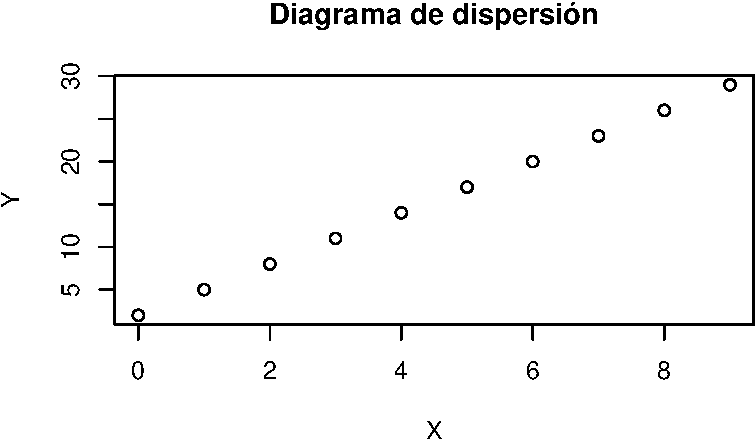
\includegraphics{05-regresion_files/figure-pdf/unnamed-chunk-2-1.pdf}

  \end{tcolorbox}

  \begin{tcolorbox}[enhanced jigsaw, toprule=.15mm, rightrule=.15mm, arc=.35mm, colback=white, colbacktitle=quarto-callout-tip-color!10!white, toptitle=1mm, left=2mm, colframe=quarto-callout-tip-color-frame, opacityback=0, breakable, opacitybacktitle=0.6, bottomtitle=1mm, titlerule=0mm, title=\textcolor{quarto-callout-tip-color}{\faLightbulb}\hspace{0.5em}{Solución 2}, bottomrule=.15mm, coltitle=black, leftrule=.75mm]

  Otra alternativa es usar la función la función
  \href{https://aprendeconalf.es/manual-r/07-graficos.html\#diagramas-de-puntos}{\texttt{geom\_point}}
  del paquete \texttt{ggplot2}.

\begin{Shaded}
\begin{Highlighting}[]
\FunctionTok{library}\NormalTok{(ggplot2)}
\FunctionTok{ggplot}\NormalTok{(df, }\FunctionTok{aes}\NormalTok{(}\AttributeTok{x =}\NormalTok{ x, }\AttributeTok{y =}\NormalTok{ y)) }\SpecialCharTok{+}
    \FunctionTok{geom\_point}\NormalTok{(}\AttributeTok{col =} \StringTok{"red"}\NormalTok{) }\SpecialCharTok{+}
    \FunctionTok{labs}\NormalTok{(}\AttributeTok{title =} \StringTok{"Diagrama de dispersión"}\NormalTok{, }\AttributeTok{x =} \StringTok{"X"}\NormalTok{, }\AttributeTok{y =} \StringTok{"Y"}\NormalTok{)}
\end{Highlighting}
\end{Shaded}

  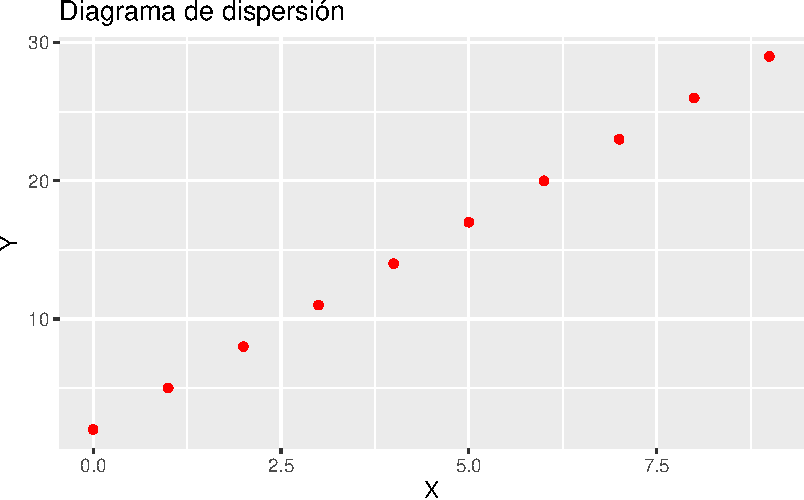
\includegraphics{05-regresion_files/figure-pdf/unnamed-chunk-3-1.pdf}

  El tipo de modelo que mejor se ajusta es lineal, ya que todos los
  puntos están alineados.

  \end{tcolorbox}
\item
  Calcular la recta de regresión de \(Y\) sobre \(X\).

  \begin{tcolorbox}[enhanced jigsaw, toprule=.15mm, rightrule=.15mm, arc=.35mm, colback=white, colbacktitle=quarto-callout-tip-color!10!white, toptitle=1mm, left=2mm, colframe=quarto-callout-tip-color-frame, opacityback=0, breakable, opacitybacktitle=0.6, bottomtitle=1mm, titlerule=0mm, title=\textcolor{quarto-callout-tip-color}{\faLightbulb}\hspace{0.5em}{Solución}, bottomrule=.15mm, coltitle=black, leftrule=.75mm]

  Para ajustar un modelo de regresión se utiliza la función
  \href{https://www.rdocumentation.org/packages/stats/versions/3.6.2/topics/lm}{\texttt{lm}}
  del paquete \texttt{stats}. Esta función requiere que se le pase como
  parámetro la fórmula del modelo de regresión que debe tener la
  sintaxis \texttt{y\ \textasciitilde{}\ f(x)}, donde \texttt{y} es la
  variable dependiente en el modelo, \texttt{x} es la variable
  independiente, y \texttt{f(x)} es una expresión matemática que
  describe el modelo.

\begin{Shaded}
\begin{Highlighting}[]
\NormalTok{recta\_y\_x }\OtherTok{\textless{}{-}} \FunctionTok{lm}\NormalTok{(y }\SpecialCharTok{\textasciitilde{}}\NormalTok{ x, df) }
\FunctionTok{summary}\NormalTok{(recta\_y\_x)}
\end{Highlighting}
\end{Shaded}

\begin{verbatim}

Call:
lm(formula = y ~ x, data = df)

Residuals:
       Min         1Q     Median         3Q        Max 
-3.675e-15 -8.783e-16  5.168e-16  9.646e-16  1.944e-15 

Coefficients:
             Estimate Std. Error   t value Pr(>|t|)    
(Intercept) 2.000e+00  1.049e-15 1.906e+15   <2e-16 ***
x           3.000e+00  1.965e-16 1.527e+16   <2e-16 ***
---
Signif. codes:  0 '***' 0.001 '**' 0.01 '*' 0.05 '.' 0.1 ' ' 1

Residual standard error: 1.785e-15 on 8 degrees of freedom
Multiple R-squared:      1, Adjusted R-squared:      1 
F-statistic: 2.33e+32 on 1 and 8 DF,  p-value: < 2.2e-16
\end{verbatim}

  La recta de regresión de \(Y\) sobre \(X\) es \(y = 2 + 3 x\).

  \end{tcolorbox}
\item
  Obtener el coeficiente de regresión de la recta anterior e
  interpretarlo.

  \begin{tcolorbox}[enhanced jigsaw, toprule=.15mm, rightrule=.15mm, arc=.35mm, colback=white, colbacktitle=quarto-callout-tip-color!10!white, toptitle=1mm, left=2mm, colframe=quarto-callout-tip-color-frame, opacityback=0, breakable, opacitybacktitle=0.6, bottomtitle=1mm, titlerule=0mm, title=\textcolor{quarto-callout-tip-color}{\faLightbulb}\hspace{0.5em}{Solución}, bottomrule=.15mm, coltitle=black, leftrule=.75mm]

  El coeficiente de regresión es la pendiente de la recta de regresión

\begin{Shaded}
\begin{Highlighting}[]
\FunctionTok{cat}\NormalTok{(}\FunctionTok{paste}\NormalTok{(}\StringTok{"Coeficiente de regresión de Y sobre X:"}\NormalTok{, recta\_y\_x}\SpecialCharTok{$}\NormalTok{coefficients[[}\StringTok{"x"}\NormalTok{]]))}
\end{Highlighting}
\end{Shaded}

\begin{verbatim}
Coeficiente de regresión de Y sobre X: 3
\end{verbatim}

  El coeficiente de regresión de \(Y\) sobre \(X\) vale 3, lo que indica
  que \(Y\) aumenta 3 unidades por cada unidad que aumenta \(X\).

  \end{tcolorbox}
\item
  Dibujar la recta de regresión de \(Y\) sobre \(X\) sobre el diagrama
  de dispersión. ¿Cómo son los residuos del modelo de regresión?

  \begin{tcolorbox}[enhanced jigsaw, toprule=.15mm, rightrule=.15mm, arc=.35mm, colback=white, colbacktitle=quarto-callout-tip-color!10!white, toptitle=1mm, left=2mm, colframe=quarto-callout-tip-color-frame, opacityback=0, breakable, opacitybacktitle=0.6, bottomtitle=1mm, titlerule=0mm, title=\textcolor{quarto-callout-tip-color}{\faLightbulb}\hspace{0.5em}{Solución 1}, bottomrule=.15mm, coltitle=black, leftrule=.75mm]

  Para dibujar la recta de regresión se puede usar la función
  \href{https://www.rdocumentation.org/packages/graphics/versions/3.6.2/topics/abline}{\texttt{abline}}
  del paquete \texttt{graphics}.

\begin{Shaded}
\begin{Highlighting}[]
\FunctionTok{plot}\NormalTok{(df}\SpecialCharTok{$}\NormalTok{x, df}\SpecialCharTok{$}\NormalTok{y, }\AttributeTok{xlab =} \StringTok{"X"}\NormalTok{, }\AttributeTok{ylab =} \StringTok{"Y"}\NormalTok{, }\AttributeTok{main =} \StringTok{"Diagrama de dispersión"}\NormalTok{)}
\FunctionTok{abline}\NormalTok{(recta\_y\_x)}
\end{Highlighting}
\end{Shaded}

  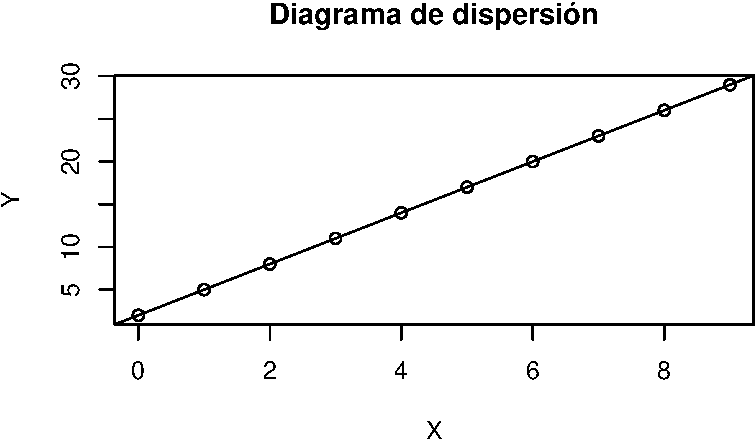
\includegraphics{05-regresion_files/figure-pdf/unnamed-chunk-6-1.pdf}

  \end{tcolorbox}

  \begin{tcolorbox}[enhanced jigsaw, toprule=.15mm, rightrule=.15mm, arc=.35mm, colback=white, colbacktitle=quarto-callout-tip-color!10!white, toptitle=1mm, left=2mm, colframe=quarto-callout-tip-color-frame, opacityback=0, breakable, opacitybacktitle=0.6, bottomtitle=1mm, titlerule=0mm, title=\textcolor{quarto-callout-tip-color}{\faLightbulb}\hspace{0.5em}{Solución 2}, bottomrule=.15mm, coltitle=black, leftrule=.75mm]

  Otra alternativa es usar la geometría de ajuste de regresión por
  mínimos cuadrados
  \href{https://aprendeconalf.es/manual-r/07-graficos.html\#interpolaci\%C3\%B3n-y-ajustes-de-regresi\%C3\%B3n}{\texttt{geom\_smooth}}
  del paquete \texttt{ggplot2}.

\begin{Shaded}
\begin{Highlighting}[]
\FunctionTok{library}\NormalTok{(ggplot2)}
\FunctionTok{ggplot}\NormalTok{(df, }\FunctionTok{aes}\NormalTok{(}\AttributeTok{x =}\NormalTok{ x, }\AttributeTok{y =}\NormalTok{ y)) }\SpecialCharTok{+}
    \FunctionTok{geom\_point}\NormalTok{(}\AttributeTok{col =} \StringTok{"red"}\NormalTok{) }\SpecialCharTok{+}
    \FunctionTok{geom\_smooth}\NormalTok{(}\AttributeTok{method =} \StringTok{"lm"}\NormalTok{) }\SpecialCharTok{+}
    \FunctionTok{labs}\NormalTok{(}\AttributeTok{title =} \StringTok{"Diagrama de dispersión"}\NormalTok{, }\AttributeTok{x =} \StringTok{"X"}\NormalTok{, }\AttributeTok{y =} \StringTok{"Y"}\NormalTok{)}
\end{Highlighting}
\end{Shaded}

  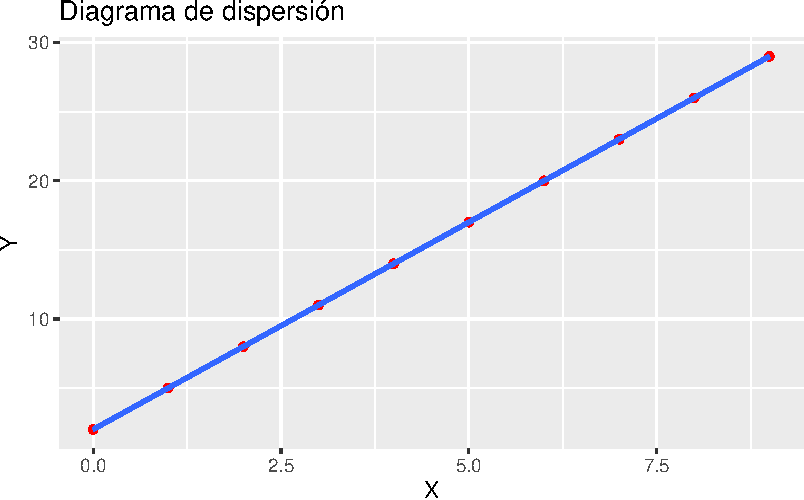
\includegraphics{05-regresion_files/figure-pdf/unnamed-chunk-7-1.pdf}

  Como la recta pasa por todos los puntos del diagrama de dispersión,
  los residuos son nulos.

  \end{tcolorbox}
\item
  Calcular el coeficiente de determinación del modelo lineal e
  interpretarlo.

  \begin{tcolorbox}[enhanced jigsaw, toprule=.15mm, rightrule=.15mm, arc=.35mm, colback=white, colbacktitle=quarto-callout-tip-color!10!white, toptitle=1mm, left=2mm, colframe=quarto-callout-tip-color-frame, opacityback=0, breakable, opacitybacktitle=0.6, bottomtitle=1mm, titlerule=0mm, title=\textcolor{quarto-callout-tip-color}{\faLightbulb}\hspace{0.5em}{Solución}, bottomrule=.15mm, coltitle=black, leftrule=.75mm]

\begin{Shaded}
\begin{Highlighting}[]
\FunctionTok{cat}\NormalTok{(}\FunctionTok{paste}\NormalTok{(}\StringTok{"Coeficiente de determinación lineal R²:"}\NormalTok{, }\FunctionTok{summary}\NormalTok{(recta\_y\_x)}\SpecialCharTok{$}\NormalTok{r.squared))}
\end{Highlighting}
\end{Shaded}

\begin{verbatim}
Coeficiente de determinación lineal R²: 1
\end{verbatim}

  Como el coeficiente de determinación lineal vale 1, el ajuste de la
  recta de regresión es perfecto.

  \end{tcolorbox}
\item
  Calcular la recta de regresión de \(X\) sobre \(Y\). ¿Coincide con la
  recta de regresión de \(Y\) sobre \(X\)?

  \begin{tcolorbox}[enhanced jigsaw, toprule=.15mm, rightrule=.15mm, arc=.35mm, colback=white, colbacktitle=quarto-callout-tip-color!10!white, toptitle=1mm, left=2mm, colframe=quarto-callout-tip-color-frame, opacityback=0, breakable, opacitybacktitle=0.6, bottomtitle=1mm, titlerule=0mm, title=\textcolor{quarto-callout-tip-color}{\faLightbulb}\hspace{0.5em}{Solución}, bottomrule=.15mm, coltitle=black, leftrule=.75mm]

\begin{Shaded}
\begin{Highlighting}[]
\NormalTok{recta\_x\_y }\OtherTok{\textless{}{-}} \FunctionTok{lm}\NormalTok{(x }\SpecialCharTok{\textasciitilde{}}\NormalTok{ y, df) }
\FunctionTok{summary}\NormalTok{(recta\_x\_y)}
\end{Highlighting}
\end{Shaded}

\begin{verbatim}

Call:
lm(formula = x ~ y, data = df)

Residuals:
       Min         1Q     Median         3Q        Max 
-1.435e-15 -5.090e-16 -2.062e-17  3.798e-16  1.943e-15 

Coefficients:
              Estimate Std. Error    t value Pr(>|t|)    
(Intercept) -6.667e-01  6.179e-16 -1.079e+15   <2e-16 ***
y            3.333e-01  3.484e-17  9.567e+15   <2e-16 ***
---
Signif. codes:  0 '***' 0.001 '**' 0.01 '*' 0.05 '.' 0.1 ' ' 1

Residual standard error: 9.494e-16 on 8 degrees of freedom
Multiple R-squared:      1, Adjusted R-squared:      1 
F-statistic: 9.153e+31 on 1 and 8 DF,  p-value: < 2.2e-16
\end{verbatim}

  La recta de regresión de \(X\) sobre \(Y\) es
  \(x = -0.6666667 + 0.3333333 x\), que es la misma que la recta de
  \(Y\) sobre \(X\), ya que el ajuste es perfecto, y tanto los residuos
  en \(Y\) como los residuos en \(X\) valen cero para esta recta.

  \end{tcolorbox}
\end{enumerate}

\end{exercise}

\begin{exercise}[]\protect\hypertarget{exr-regresion-2}{}\label{exr-regresion-2}

El fichero \href{datos/horas-estudio.csv}{\texttt{horas-estudio.csv}}
contiene información sobre las horas de estudio diarias de una muestra
de alumnos de ingeniería, y el número de asignaturas suspendidas al
final del curso.

\begin{enumerate}
\def\labelenumi{\alph{enumi}.}
\item
  Crear un data frame con los datos de las horas de estudio y los
  suspensos a partir del fichero
  \href{https://aprendeconalf.es/estadistica-practicas-r/datos/horas-estudio.csv}{\texttt{horas-estudio.csv}}.

  \begin{tcolorbox}[enhanced jigsaw, toprule=.15mm, rightrule=.15mm, arc=.35mm, colback=white, colbacktitle=quarto-callout-tip-color!10!white, toptitle=1mm, left=2mm, colframe=quarto-callout-tip-color-frame, opacityback=0, breakable, opacitybacktitle=0.6, bottomtitle=1mm, titlerule=0mm, title=\textcolor{quarto-callout-tip-color}{\faLightbulb}\hspace{0.5em}{Solución}, bottomrule=.15mm, coltitle=black, leftrule=.75mm]

\begin{Shaded}
\begin{Highlighting}[]
\FunctionTok{library}\NormalTok{(readr)}
\NormalTok{df }\OtherTok{\textless{}{-}} \FunctionTok{read\_csv}\NormalTok{(}\StringTok{"https://aprendeconalf.es/estadistica{-}practicas{-}r/datos/horas{-}estudio.csv"}\NormalTok{)}
\NormalTok{df}
\end{Highlighting}
\end{Shaded}

\begin{verbatim}
# A tibble: 30 x 2
   Horas Suspensos
   <dbl>     <dbl>
 1   3.5         1
 2   0.6         5
 3   2.8         1
 4   2.5         3
 5   2.6         1
 6   3.9         0
 7   1.5         3
 8   0.7         3
 9   3.6         1
10   3.7         1
# i 20 more rows
\end{verbatim}

  \end{tcolorbox}
\item
  Dibujar el diagrama de dispersión correspondiente. ¿Qué tipo de modelo
  de regresión se ajusta mejor a la nube de puntos?

  \begin{tcolorbox}[enhanced jigsaw, toprule=.15mm, rightrule=.15mm, arc=.35mm, colback=white, colbacktitle=quarto-callout-tip-color!10!white, toptitle=1mm, left=2mm, colframe=quarto-callout-tip-color-frame, opacityback=0, breakable, opacitybacktitle=0.6, bottomtitle=1mm, titlerule=0mm, title=\textcolor{quarto-callout-tip-color}{\faLightbulb}\hspace{0.5em}{Solución}, bottomrule=.15mm, coltitle=black, leftrule=.75mm]

\begin{Shaded}
\begin{Highlighting}[]
\FunctionTok{library}\NormalTok{(ggplot2)}
\FunctionTok{ggplot}\NormalTok{(df, }\FunctionTok{aes}\NormalTok{(}\AttributeTok{x =}\NormalTok{ Horas, }\AttributeTok{y =}\NormalTok{ Suspensos)) }\SpecialCharTok{+}
    \FunctionTok{geom\_point}\NormalTok{(}\AttributeTok{col =} \StringTok{"red"}\NormalTok{) }\SpecialCharTok{+}
    \FunctionTok{labs}\NormalTok{(}\AttributeTok{title =} \StringTok{"Diagrama de dispersión"}\NormalTok{, }\AttributeTok{x =} \StringTok{"Horas de estudio"}\NormalTok{, }\AttributeTok{y =} \StringTok{"Asignaturas suspensas"}\NormalTok{)}
\end{Highlighting}
\end{Shaded}

  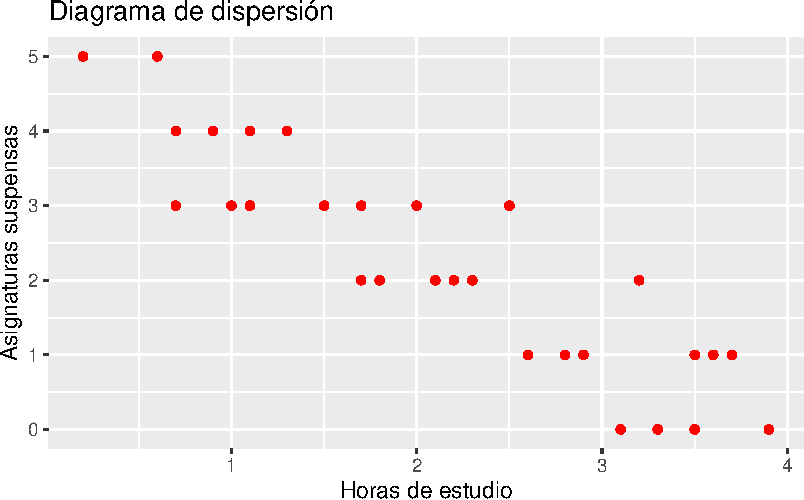
\includegraphics{05-regresion_files/figure-pdf/unnamed-chunk-11-1.pdf}

  El tipo de modelo que mejor se ajusta es lineal, ya que hay una
  tendencia lineal en la nube de puntos y además es inversa.

  \end{tcolorbox}
\item
  Calcular la recta de regresión de los suspensos sobre las horas de
  estudio.

  \begin{tcolorbox}[enhanced jigsaw, toprule=.15mm, rightrule=.15mm, arc=.35mm, colback=white, colbacktitle=quarto-callout-tip-color!10!white, toptitle=1mm, left=2mm, colframe=quarto-callout-tip-color-frame, opacityback=0, breakable, opacitybacktitle=0.6, bottomtitle=1mm, titlerule=0mm, title=\textcolor{quarto-callout-tip-color}{\faLightbulb}\hspace{0.5em}{Solución}, bottomrule=.15mm, coltitle=black, leftrule=.75mm]

\begin{Shaded}
\begin{Highlighting}[]
\NormalTok{recta\_suspensos\_horas }\OtherTok{\textless{}{-}} \FunctionTok{lm}\NormalTok{(Suspensos }\SpecialCharTok{\textasciitilde{}}\NormalTok{ Horas, df) }
\FunctionTok{summary}\NormalTok{(recta\_suspensos\_horas)}
\end{Highlighting}
\end{Shaded}

\begin{verbatim}

Call:
lm(formula = Suspensos ~ Horas, data = df)

Residuals:
     Min       1Q   Median       3Q      Max 
-1.03614 -0.53214 -0.02013  0.49187  1.22587 

Coefficients:
            Estimate Std. Error t value Pr(>|t|)    
(Intercept)   4.8491     0.2622   18.49  < 2e-16 ***
Horas        -1.2300     0.1106  -11.12  8.7e-12 ***
---
Signif. codes:  0 '***' 0.001 '**' 0.01 '*' 0.05 '.' 0.1 ' ' 1

Residual standard error: 0.6359 on 28 degrees of freedom
Multiple R-squared:  0.8155,    Adjusted R-squared:  0.8089 
F-statistic: 123.8 on 1 and 28 DF,  p-value: 8.7e-12
\end{verbatim}

  La recta de regresión de los suspensos sobre las horas es
  \(\textsf{suspensos}= 4.8491273 + -1.2299972 \textsf{horas}\).

  \end{tcolorbox}
\item
  Obtener el coeficiente de regresión de la recta anterior e
  interpretarlo.

  \begin{tcolorbox}[enhanced jigsaw, toprule=.15mm, rightrule=.15mm, arc=.35mm, colback=white, colbacktitle=quarto-callout-tip-color!10!white, toptitle=1mm, left=2mm, colframe=quarto-callout-tip-color-frame, opacityback=0, breakable, opacitybacktitle=0.6, bottomtitle=1mm, titlerule=0mm, title=\textcolor{quarto-callout-tip-color}{\faLightbulb}\hspace{0.5em}{Solución}, bottomrule=.15mm, coltitle=black, leftrule=.75mm]

\begin{Shaded}
\begin{Highlighting}[]
\FunctionTok{cat}\NormalTok{(}\FunctionTok{paste}\NormalTok{(}\StringTok{"Coeficiente de regresión de Suspensos sobre Horas:"}\NormalTok{, recta\_suspensos\_horas}\SpecialCharTok{$}\NormalTok{coefficients[[}\StringTok{"Horas"}\NormalTok{]]))}
\end{Highlighting}
\end{Shaded}

\begin{verbatim}
Coeficiente de regresión de Suspensos sobre Horas: -1.22999717844331
\end{verbatim}

  El coeficiente de regresión de los suspensos sobre las horas de
  estudio vale -1.2299972, lo que indica que por cada hora de estudio se
  obtendrán 1.2299972 suspensos menos al final del curso.

  \end{tcolorbox}
\item
  Dibujar la recta de regresión sobre el diagrama de dispersión. ¿El
  ajuste es mejor o peor que el del ejercicio anterior?

  \begin{tcolorbox}[enhanced jigsaw, toprule=.15mm, rightrule=.15mm, arc=.35mm, colback=white, colbacktitle=quarto-callout-tip-color!10!white, toptitle=1mm, left=2mm, colframe=quarto-callout-tip-color-frame, opacityback=0, breakable, opacitybacktitle=0.6, bottomtitle=1mm, titlerule=0mm, title=\textcolor{quarto-callout-tip-color}{\faLightbulb}\hspace{0.5em}{Solución}, bottomrule=.15mm, coltitle=black, leftrule=.75mm]

\begin{Shaded}
\begin{Highlighting}[]
\FunctionTok{library}\NormalTok{(ggplot2)}
\FunctionTok{ggplot}\NormalTok{(df, }\FunctionTok{aes}\NormalTok{(}\AttributeTok{x =}\NormalTok{ Horas, }\AttributeTok{y =}\NormalTok{ Suspensos)) }\SpecialCharTok{+}
    \FunctionTok{geom\_point}\NormalTok{(}\AttributeTok{col =} \StringTok{"red"}\NormalTok{) }\SpecialCharTok{+}
    \FunctionTok{geom\_smooth}\NormalTok{(}\AttributeTok{method =} \StringTok{"lm"}\NormalTok{) }\SpecialCharTok{+}
    \FunctionTok{labs}\NormalTok{(}\AttributeTok{title =} \StringTok{"Diagrama de dispersión"}\NormalTok{, }\AttributeTok{x =} \StringTok{"Horas de estudio"}\NormalTok{, }\AttributeTok{y =} \StringTok{"Asignaturas suspensas"}\NormalTok{)}
\end{Highlighting}
\end{Shaded}

  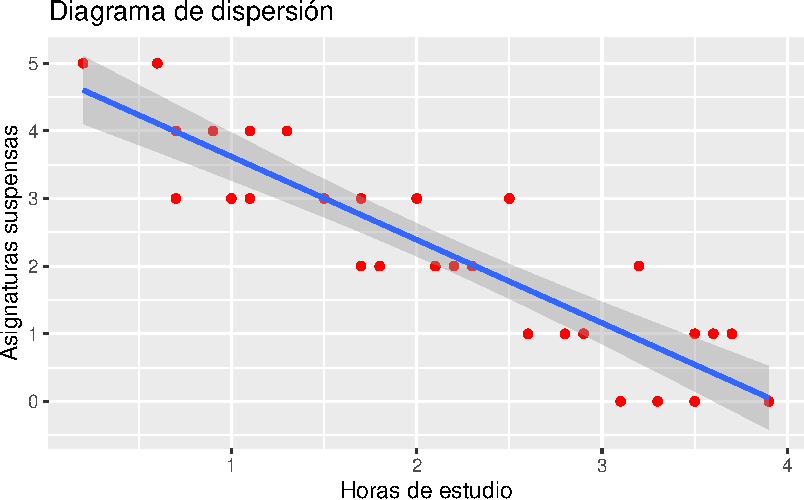
\includegraphics{05-regresion_files/figure-pdf/unnamed-chunk-14-1.pdf}

  En este caso el ajuste no es perfecto, ya que es imposible que la
  recta pase por todos los puntos como ocurría en el ejercicio anterior.
  Por tanto, el ajuste es peor.

  \end{tcolorbox}
\item
  Calcular el coeficiente de determinación del modelo lineal e
  interpretarlo.

  \begin{tcolorbox}[enhanced jigsaw, toprule=.15mm, rightrule=.15mm, arc=.35mm, colback=white, colbacktitle=quarto-callout-tip-color!10!white, toptitle=1mm, left=2mm, colframe=quarto-callout-tip-color-frame, opacityback=0, breakable, opacitybacktitle=0.6, bottomtitle=1mm, titlerule=0mm, title=\textcolor{quarto-callout-tip-color}{\faLightbulb}\hspace{0.5em}{Solución}, bottomrule=.15mm, coltitle=black, leftrule=.75mm]

\begin{Shaded}
\begin{Highlighting}[]
\FunctionTok{cat}\NormalTok{(}\FunctionTok{paste}\NormalTok{(}\StringTok{"Coeficiente de determinación lineal R²:"}\NormalTok{, }\FunctionTok{summary}\NormalTok{(recta\_suspensos\_horas)}\SpecialCharTok{$}\NormalTok{r.squared))}
\end{Highlighting}
\end{Shaded}

\begin{verbatim}
Coeficiente de determinación lineal R²: 0.81549948723949
\end{verbatim}

  Como el coeficiente de determinación lineal vale 0.8154995 que está
  bastante próximo a 1, el ajuste es bueno, y el modelo puede utilizarse
  con fines predictivos.

  \end{tcolorbox}
\item
  Utilizar la recta de regresión para predecir el número de suspensos
  correspondiente a 3 horas de estudio diarias. ¿Es fiable esta
  predicción?

  \begin{tcolorbox}[enhanced jigsaw, toprule=.15mm, rightrule=.15mm, arc=.35mm, colback=white, colbacktitle=quarto-callout-tip-color!10!white, toptitle=1mm, left=2mm, colframe=quarto-callout-tip-color-frame, opacityback=0, breakable, opacitybacktitle=0.6, bottomtitle=1mm, titlerule=0mm, title=\textcolor{quarto-callout-tip-color}{\faLightbulb}\hspace{0.5em}{Solución}, bottomrule=.15mm, coltitle=black, leftrule=.75mm]

\begin{Shaded}
\begin{Highlighting}[]
\FunctionTok{predict.lm}\NormalTok{(recta\_suspensos\_horas, }\AttributeTok{newdata =} \FunctionTok{list}\NormalTok{(}\AttributeTok{Horas =} \DecValTok{3}\NormalTok{))}
\end{Highlighting}
\end{Shaded}

\begin{verbatim}
       1 
1.159136 
\end{verbatim}

  La predicción será fiable ya que el coeficiente de determinación está
  próximo a 1 y el tamaño de la muestra no es muy pequeño.

  \end{tcolorbox}
\item
  Según el modelo lineal, ¿cuántas horas diarias tendrá que estudiar
  como mínimo un alumno si quiere aprobarlo todo?

  \begin{tcolorbox}[enhanced jigsaw, toprule=.15mm, rightrule=.15mm, arc=.35mm, colback=white, colbacktitle=quarto-callout-tip-color!10!white, toptitle=1mm, left=2mm, colframe=quarto-callout-tip-color-frame, opacityback=0, breakable, opacitybacktitle=0.6, bottomtitle=1mm, titlerule=0mm, title=\textcolor{quarto-callout-tip-color}{\faLightbulb}\hspace{0.5em}{Solución}, bottomrule=.15mm, coltitle=black, leftrule=.75mm]

  Como ahora queremos predecir el número de horas de estudio,
  necesitamos calcular la recta de regresión de la horas sobre los
  suspensos.

\begin{Shaded}
\begin{Highlighting}[]
\NormalTok{recta\_horas\_suspensos }\OtherTok{\textless{}{-}} \FunctionTok{lm}\NormalTok{(Horas }\SpecialCharTok{\textasciitilde{}}\NormalTok{ Suspensos, df) }
\FunctionTok{predict.lm}\NormalTok{(recta\_horas\_suspensos, }\AttributeTok{newdata =} \FunctionTok{list}\NormalTok{(}\AttributeTok{Suspensos =} \DecValTok{0}\NormalTok{))}
\end{Highlighting}
\end{Shaded}

\begin{verbatim}
       1 
3.607387 
\end{verbatim}

  \end{tcolorbox}
\end{enumerate}

\end{exercise}

\begin{exercise}[]\protect\hypertarget{exr-regresion-3}{}\label{exr-regresion-3}

Después de tomar un litro de vino se ha medido la concentración de
alcohol en la sangre en distintos instantes, obteniendo los siguientes
datos

\[
\begin{array}{lrrrrrrr}
\hline 
\mbox{Tiempo después (minutos)} & 30 & 60 & 90 & 120 & 150 & 180 & 210\\ 
\mbox{Alcohol (gramos/litro)} & 1.6 & 1.7 & 1.5 & 1.1 & 0.7 & 0.2 & 2.1\\
\hline
\end{array}
\]

\begin{enumerate}
\def\labelenumi{\alph{enumi}.}
\item
  Crear un data frame con los datos del tiempo y la concentración de
  alcohol.

  \begin{tcolorbox}[enhanced jigsaw, toprule=.15mm, rightrule=.15mm, arc=.35mm, colback=white, colbacktitle=quarto-callout-tip-color!10!white, toptitle=1mm, left=2mm, colframe=quarto-callout-tip-color-frame, opacityback=0, breakable, opacitybacktitle=0.6, bottomtitle=1mm, titlerule=0mm, title=\textcolor{quarto-callout-tip-color}{\faLightbulb}\hspace{0.5em}{Solución}, bottomrule=.15mm, coltitle=black, leftrule=.75mm]

\begin{Shaded}
\begin{Highlighting}[]
\NormalTok{df }\OtherTok{\textless{}{-}} \FunctionTok{data.frame}\NormalTok{(}
    \AttributeTok{Tiempo =} \FunctionTok{c}\NormalTok{(}\DecValTok{30}\NormalTok{, }\DecValTok{60}\NormalTok{, }\DecValTok{90}\NormalTok{, }\DecValTok{120}\NormalTok{, }\DecValTok{150}\NormalTok{, }\DecValTok{180}\NormalTok{, }\DecValTok{210}\NormalTok{),}
    \AttributeTok{Alcohol =} \FunctionTok{c}\NormalTok{(}\FloatTok{1.6}\NormalTok{, }\FloatTok{1.7}\NormalTok{, }\FloatTok{1.5}\NormalTok{, }\FloatTok{1.1}\NormalTok{, }\FloatTok{0.7}\NormalTok{, }\FloatTok{0.2}\NormalTok{, }\FloatTok{2.1}\NormalTok{)}
\NormalTok{)}
\NormalTok{df}
\end{Highlighting}
\end{Shaded}

\begin{verbatim}
  Tiempo Alcohol
1     30     1.6
2     60     1.7
3     90     1.5
4    120     1.1
5    150     0.7
6    180     0.2
7    210     2.1
\end{verbatim}

  \end{tcolorbox}
\item
  Calcular el coeficiente de correlación lineal. ¿Existe relación lineal
  entre la concentración de alcohol y el tiempo que pasa?

  \begin{tcolorbox}[enhanced jigsaw, toprule=.15mm, rightrule=.15mm, arc=.35mm, colback=white, colbacktitle=quarto-callout-tip-color!10!white, toptitle=1mm, left=2mm, colframe=quarto-callout-tip-color-frame, opacityback=0, breakable, opacitybacktitle=0.6, bottomtitle=1mm, titlerule=0mm, title=\textcolor{quarto-callout-tip-color}{\faLightbulb}\hspace{0.5em}{Solución}, bottomrule=.15mm, coltitle=black, leftrule=.75mm]

  Para calcular el coeficiente de correlación lineal de Pearson se puede
  utilar la función
  \href{https://www.rdocumentation.org/packages/stats/versions/3.6.2/topics/cor}{\texttt{cor}}
  del paquete \texttt{stats}.

\begin{Shaded}
\begin{Highlighting}[]
\FunctionTok{cor}\NormalTok{(df}\SpecialCharTok{$}\NormalTok{Tiempo, df}\SpecialCharTok{$}\NormalTok{Alcohol)}
\end{Highlighting}
\end{Shaded}

\begin{verbatim}
[1] -0.2730367
\end{verbatim}

  El valore del coeficiente de correlación lineal es muy bajo, por lo
  que aparentemente no hay relación lineal entre la concentración de
  alcohol en sangre y el tiempo que pasa.

  \end{tcolorbox}
\item
  Dibujar el diagrama de dispersión correspondiente y la recta de
  regresión de la concentración de alcohol sobre el tiempo. ¿Por qué el
  ajuste es tan malo?

  \begin{tcolorbox}[enhanced jigsaw, toprule=.15mm, rightrule=.15mm, arc=.35mm, colback=white, colbacktitle=quarto-callout-tip-color!10!white, toptitle=1mm, left=2mm, colframe=quarto-callout-tip-color-frame, opacityback=0, breakable, opacitybacktitle=0.6, bottomtitle=1mm, titlerule=0mm, title=\textcolor{quarto-callout-tip-color}{\faLightbulb}\hspace{0.5em}{Solución}, bottomrule=.15mm, coltitle=black, leftrule=.75mm]

\begin{Shaded}
\begin{Highlighting}[]
\FunctionTok{library}\NormalTok{(ggplot2)}
\FunctionTok{ggplot}\NormalTok{(df, }\FunctionTok{aes}\NormalTok{(}\AttributeTok{x =}\NormalTok{ Tiempo, }\AttributeTok{y =}\NormalTok{ Alcohol)) }\SpecialCharTok{+}
    \FunctionTok{geom\_point}\NormalTok{(}\AttributeTok{col =} \StringTok{"red"}\NormalTok{) }\SpecialCharTok{+}
    \FunctionTok{geom\_smooth}\NormalTok{(}\AttributeTok{method =} \StringTok{"lm"}\NormalTok{) }\SpecialCharTok{+}
    \FunctionTok{labs}\NormalTok{(}\AttributeTok{title =} \StringTok{"Diagrama de dispersión"}\NormalTok{, }\AttributeTok{x =} \StringTok{"Tiempo en minutos"}\NormalTok{, }\AttributeTok{y =} \StringTok{"Concentración de alcohol en sangre (g/l)"}\NormalTok{)}
\end{Highlighting}
\end{Shaded}

  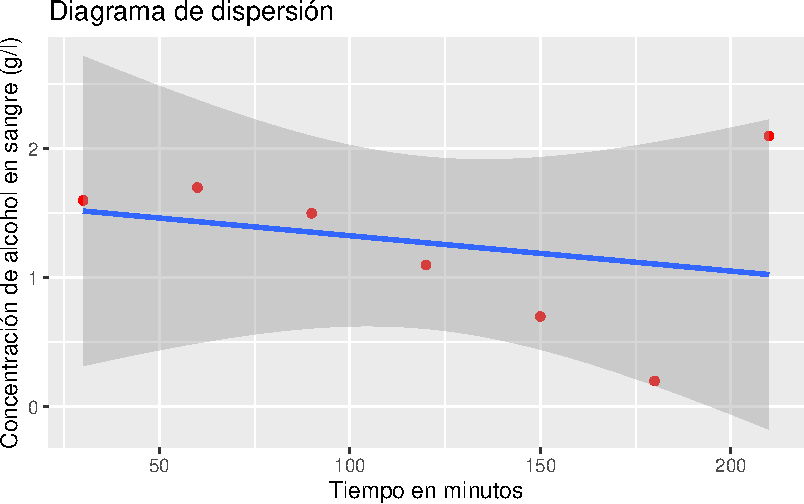
\includegraphics{05-regresion_files/figure-pdf/unnamed-chunk-20-1.pdf}

  El ajuste es malo porque hay un dato atípico que no sigue la misma
  tendencia que el resto.

  \end{tcolorbox}
\item
  Eliminar el dato atípico y calcular la recta de la concentración de
  alcohol sobre el tiempo. ¿Ha mejorado el modelo?

  \begin{tcolorbox}[enhanced jigsaw, toprule=.15mm, rightrule=.15mm, arc=.35mm, colback=white, colbacktitle=quarto-callout-tip-color!10!white, toptitle=1mm, left=2mm, colframe=quarto-callout-tip-color-frame, opacityback=0, breakable, opacitybacktitle=0.6, bottomtitle=1mm, titlerule=0mm, title=\textcolor{quarto-callout-tip-color}{\faLightbulb}\hspace{0.5em}{Solución}, bottomrule=.15mm, coltitle=black, leftrule=.75mm]

\begin{Shaded}
\begin{Highlighting}[]
\CommentTok{\# Eliminamos el dato atípico que está en la fila }
\NormalTok{df }\OtherTok{\textless{}{-}}\NormalTok{ df[}\SpecialCharTok{{-}}\FunctionTok{c}\NormalTok{(}\DecValTok{7}\NormalTok{), ]}
\NormalTok{recta\_alcohol\_tiempo }\OtherTok{\textless{}{-}} \FunctionTok{lm}\NormalTok{(Alcohol }\SpecialCharTok{\textasciitilde{}}\NormalTok{ Tiempo, df) }
\FunctionTok{summary}\NormalTok{(recta\_alcohol\_tiempo)}
\end{Highlighting}
\end{Shaded}

\begin{verbatim}

Call:
lm(formula = Alcohol ~ Tiempo, data = df)

Residuals:
       1        2        3        4        5        6 
-0.27619  0.12095  0.21810  0.11524  0.01238 -0.19048 

Coefficients:
             Estimate Std. Error t value Pr(>|t|)    
(Intercept)  2.173333   0.201927  10.763 0.000423 ***
Tiempo      -0.009905   0.001728  -5.731 0.004591 ** 
---
Signif. codes:  0 '***' 0.001 '**' 0.01 '*' 0.05 '.' 0.1 ' ' 1

Residual standard error: 0.2169 on 4 degrees of freedom
Multiple R-squared:  0.8914,    Adjusted R-squared:  0.8643 
F-statistic: 32.84 on 1 and 4 DF,  p-value: 0.004591
\end{verbatim}

  La recta de regresión de la concentración de alcohol en sangre sobre
  el tiempo es
  \(\textsf{alcohol}= 2.1733333 + -0.0099048 \textsf{tiempo}\).

  El modelo ha mejorado notablemente ya que ahora el coeficiente de
  determinación lineal \(R^2=0.8914286\), que está muy próximo a 1.

  \end{tcolorbox}
\item
  Según el modelo de regresión lineal, ¿a qué velocidad metaboliza esta
  persona el alcohol?

  \begin{tcolorbox}[enhanced jigsaw, toprule=.15mm, rightrule=.15mm, arc=.35mm, colback=white, colbacktitle=quarto-callout-tip-color!10!white, toptitle=1mm, left=2mm, colframe=quarto-callout-tip-color-frame, opacityback=0, breakable, opacitybacktitle=0.6, bottomtitle=1mm, titlerule=0mm, title=\textcolor{quarto-callout-tip-color}{\faLightbulb}\hspace{0.5em}{Solución}, bottomrule=.15mm, coltitle=black, leftrule=.75mm]

\begin{Shaded}
\begin{Highlighting}[]
\FunctionTok{cat}\NormalTok{(}\FunctionTok{paste}\NormalTok{(}\StringTok{"Coeficiente de regresión de la concentración de alchol sobre el tiempo:"}\NormalTok{, recta\_alcohol\_tiempo}\SpecialCharTok{$}\NormalTok{coefficients[[}\StringTok{"Tiempo"}\NormalTok{]]))}
\end{Highlighting}
\end{Shaded}

\begin{verbatim}
Coeficiente de regresión de la concentración de alchol sobre el tiempo: -0.00990476190476191
\end{verbatim}

  Así pues, la velocidad de metabolización del alcohol es 0.0099048
  g/l\(\cdot\)min.

  \end{tcolorbox}
\item
  Si la concentración máxima de alcohol en la sangre que permite la ley
  para poder conducir es \(0.3\) g/l, ¿cuánto tiempo habrá que esperar
  después de tomarse un litro de vino para poder conducir sin infringir
  la ley? ¿Es fiable esta predicción?

  \begin{tcolorbox}[enhanced jigsaw, toprule=.15mm, rightrule=.15mm, arc=.35mm, colback=white, colbacktitle=quarto-callout-tip-color!10!white, toptitle=1mm, left=2mm, colframe=quarto-callout-tip-color-frame, opacityback=0, breakable, opacitybacktitle=0.6, bottomtitle=1mm, titlerule=0mm, title=\textcolor{quarto-callout-tip-color}{\faLightbulb}\hspace{0.5em}{Solución}, bottomrule=.15mm, coltitle=black, leftrule=.75mm]

  Como ahora queremos predecir el tiempo, necesitamos calcular la recta
  de regresión del tiempo sobre la concentración de alcohol.

\begin{Shaded}
\begin{Highlighting}[]
\NormalTok{recta\_tiempo\_alcohol }\OtherTok{\textless{}{-}} \FunctionTok{lm}\NormalTok{(Tiempo }\SpecialCharTok{\textasciitilde{}}\NormalTok{ Alcohol, df) }
\FunctionTok{predict.lm}\NormalTok{(recta\_tiempo\_alcohol, }\AttributeTok{newdata =} \FunctionTok{list}\NormalTok{(}\AttributeTok{Alcohol =} \FloatTok{0.3}\NormalTok{))}
\end{Highlighting}
\end{Shaded}

\begin{verbatim}
  1 
180 
\end{verbatim}

  Aunque el coeficiente de determinación lineal está próximo a 1, el
  tamaño muestral es demasiado pequeño para que la predicción sea
  fiable.

  \end{tcolorbox}
\end{enumerate}

\end{exercise}

\begin{exercise}[]\protect\hypertarget{exr-regresion-4}{}\label{exr-regresion-4}

El fichero \href{datos/pib-usa.csv}{\texttt{pib-usa.csv}} contiene
información sobre el producto interior bruto de Estados Unidos en
billones de dólares americanos desde 1947 hasta 2022.

\begin{enumerate}
\def\labelenumi{\alph{enumi}.}
\item
  Crear un data frame con los datos del PIB y los años a partir del
  fichero
  \href{https://aprendeconalf.es/estadistica-practicas-r/datos/horas-estudio.csv}{\texttt{pib-usa.csv}}.

  \begin{tcolorbox}[enhanced jigsaw, toprule=.15mm, rightrule=.15mm, arc=.35mm, colback=white, colbacktitle=quarto-callout-tip-color!10!white, toptitle=1mm, left=2mm, colframe=quarto-callout-tip-color-frame, opacityback=0, breakable, opacitybacktitle=0.6, bottomtitle=1mm, titlerule=0mm, title=\textcolor{quarto-callout-tip-color}{\faLightbulb}\hspace{0.5em}{Solución}, bottomrule=.15mm, coltitle=black, leftrule=.75mm]

\begin{Shaded}
\begin{Highlighting}[]
\FunctionTok{library}\NormalTok{(readr)}
\NormalTok{df }\OtherTok{\textless{}{-}} \FunctionTok{read\_csv}\NormalTok{(}\StringTok{"https://aprendeconalf.es/estadistica{-}practicas{-}r/datos/pib{-}usa.csv"}\NormalTok{)}
\NormalTok{df}
\end{Highlighting}
\end{Shaded}

\begin{verbatim}
# A tibble: 76 x 2
     Año   PIB
   <dbl> <dbl>
 1  1947  244.
 2  1948  267.
 3  1949  276.
 4  1950  282.
 5  1951  338.
 6  1952  362.
 7  1953  390.
 8  1954  387.
 9  1955  415.
10  1956  443.
# i 66 more rows
\end{verbatim}

  \end{tcolorbox}
\item
  Dibujar el diagrama de dispersión que represente la evolución anual
  del PIB. ¿Qué tipo de modelo de regresión se ajusta mejor a la nube de
  puntos?

  \begin{tcolorbox}[enhanced jigsaw, toprule=.15mm, rightrule=.15mm, arc=.35mm, colback=white, colbacktitle=quarto-callout-tip-color!10!white, toptitle=1mm, left=2mm, colframe=quarto-callout-tip-color-frame, opacityback=0, breakable, opacitybacktitle=0.6, bottomtitle=1mm, titlerule=0mm, title=\textcolor{quarto-callout-tip-color}{\faLightbulb}\hspace{0.5em}{Solución}, bottomrule=.15mm, coltitle=black, leftrule=.75mm]

\begin{Shaded}
\begin{Highlighting}[]
\FunctionTok{library}\NormalTok{(ggplot2)}
\FunctionTok{ggplot}\NormalTok{(df, }\FunctionTok{aes}\NormalTok{(}\AttributeTok{x =}\NormalTok{ Año, }\AttributeTok{y =}\NormalTok{ PIB)) }\SpecialCharTok{+}
    \FunctionTok{geom\_point}\NormalTok{(}\AttributeTok{col =} \StringTok{"red"}\NormalTok{) }\SpecialCharTok{+}
    \FunctionTok{labs}\NormalTok{(}\AttributeTok{title =} \StringTok{"Evolución del PIB de Estados Unidos"}\NormalTok{, }\AttributeTok{x =} \StringTok{"Año"}\NormalTok{, }\AttributeTok{y =} \StringTok{"PIB en billones dólares"}\NormalTok{)}
\end{Highlighting}
\end{Shaded}

  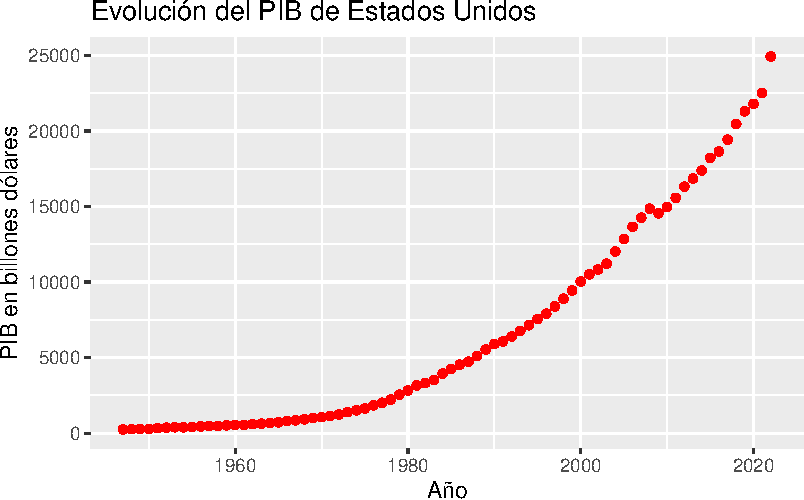
\includegraphics{05-regresion_files/figure-pdf/unnamed-chunk-25-1.pdf}

  A la vista de la forma de la nube de puntos parece que la evolución
  del PIB es exponencial.

  \end{tcolorbox}
\item
  Dibujar el diagrama de dispersión del logaritmo del PIB y los años.

  \begin{tcolorbox}[enhanced jigsaw, toprule=.15mm, rightrule=.15mm, arc=.35mm, colback=white, colbacktitle=quarto-callout-tip-color!10!white, toptitle=1mm, left=2mm, colframe=quarto-callout-tip-color-frame, opacityback=0, breakable, opacitybacktitle=0.6, bottomtitle=1mm, titlerule=0mm, title=\textcolor{quarto-callout-tip-color}{\faLightbulb}\hspace{0.5em}{Solución}, bottomrule=.15mm, coltitle=black, leftrule=.75mm]

\begin{Shaded}
\begin{Highlighting}[]
\FunctionTok{library}\NormalTok{(dplyr)}
\NormalTok{df }\OtherTok{\textless{}{-}} \FunctionTok{mutate}\NormalTok{(df, }\AttributeTok{logPIB =} \FunctionTok{log}\NormalTok{(PIB)) }
\FunctionTok{ggplot}\NormalTok{(df, }\FunctionTok{aes}\NormalTok{(}\AttributeTok{x =}\NormalTok{ Año, }\AttributeTok{y =}\NormalTok{ logPIB)) }\SpecialCharTok{+}
        \FunctionTok{geom\_point}\NormalTok{(}\AttributeTok{col =} \StringTok{"red"}\NormalTok{) }\SpecialCharTok{+}
        \FunctionTok{labs}\NormalTok{(}\AttributeTok{title =} \StringTok{"Evolución del PIB de Estados Unidos"}\NormalTok{, }\AttributeTok{x =} \StringTok{"Año"}\NormalTok{, }\AttributeTok{y =} \StringTok{"Logaritmo del PIB en billones dólares"}\NormalTok{)}
\end{Highlighting}
\end{Shaded}

  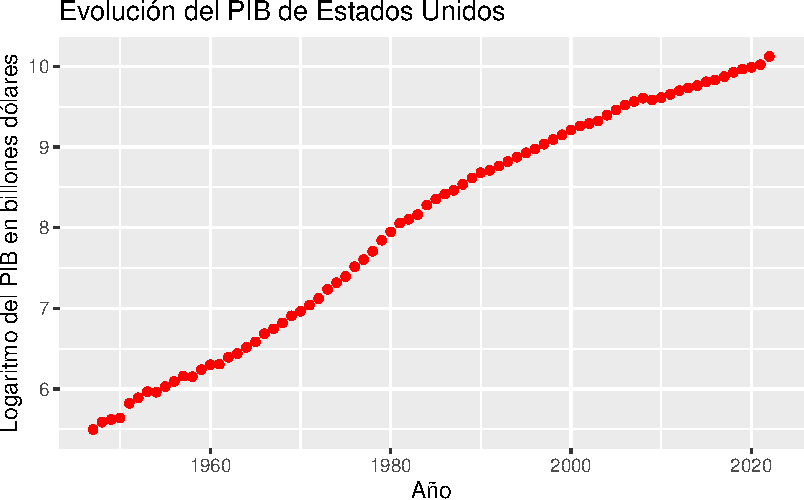
\includegraphics{05-regresion_files/figure-pdf/unnamed-chunk-26-1.pdf}

  La nube de puntos tienen una clara forma lineal, lo que confirma que
  la evolución del PIB es exponencial.

  \end{tcolorbox}
\item
  Calcular el modelo de regresión exponencial del PIB sobre los años.

  \begin{tcolorbox}[enhanced jigsaw, toprule=.15mm, rightrule=.15mm, arc=.35mm, colback=white, colbacktitle=quarto-callout-tip-color!10!white, toptitle=1mm, left=2mm, colframe=quarto-callout-tip-color-frame, opacityback=0, breakable, opacitybacktitle=0.6, bottomtitle=1mm, titlerule=0mm, title=\textcolor{quarto-callout-tip-color}{\faLightbulb}\hspace{0.5em}{Solución}, bottomrule=.15mm, coltitle=black, leftrule=.75mm]

\begin{Shaded}
\begin{Highlighting}[]
\NormalTok{recta\_logPIB\_años }\OtherTok{\textless{}{-}} \FunctionTok{lm}\NormalTok{(}\FunctionTok{log}\NormalTok{(PIB) }\SpecialCharTok{\textasciitilde{}}\NormalTok{ Año, df) }
\FunctionTok{summary}\NormalTok{(recta\_logPIB\_años)}
\end{Highlighting}
\end{Shaded}

\begin{verbatim}

Call:
lm(formula = log(PIB) ~ Año, data = df)

Residuals:
     Min       1Q   Median       3Q      Max 
-0.39115 -0.13495 -0.03532  0.17693  0.29436 

Coefficients:
              Estimate Std. Error t value Pr(>|t|)    
(Intercept) -1.215e+02  1.951e+00  -62.27   <2e-16 ***
Año          6.527e-02  9.832e-04   66.39   <2e-16 ***
---
Signif. codes:  0 '***' 0.001 '**' 0.01 '*' 0.05 '.' 0.1 ' ' 1

Residual standard error: 0.188 on 74 degrees of freedom
Multiple R-squared:  0.9835,    Adjusted R-squared:  0.9833 
F-statistic:  4407 on 1 and 74 DF,  p-value: < 2.2e-16
\end{verbatim}

  El modelo de regresión exponencial que mejor explica la evolución del
  PIB es \(\textsf{PIB}= e^{-121.4998223 + 0.065271 \textsf{Año}}\).

  \end{tcolorbox}
\item
  ¿Cuál es la tasa de crecimiento porcentual anual del PIB?

  \begin{tcolorbox}[enhanced jigsaw, toprule=.15mm, rightrule=.15mm, arc=.35mm, colback=white, colbacktitle=quarto-callout-tip-color!10!white, toptitle=1mm, left=2mm, colframe=quarto-callout-tip-color-frame, opacityback=0, breakable, opacitybacktitle=0.6, bottomtitle=1mm, titlerule=0mm, title=\textcolor{quarto-callout-tip-color}{\faLightbulb}\hspace{0.5em}{Solución}, bottomrule=.15mm, coltitle=black, leftrule=.75mm]

\begin{Shaded}
\begin{Highlighting}[]
\FunctionTok{cat}\NormalTok{(}\FunctionTok{paste}\NormalTok{(}\StringTok{"Coeficiente de regresión del logaritmo del PIB sobre los años:"}\NormalTok{, recta\_logPIB\_años}\SpecialCharTok{$}\NormalTok{coefficients[[}\StringTok{"Año"}\NormalTok{]]))}
\end{Highlighting}
\end{Shaded}

\begin{verbatim}
Coeficiente de regresión del logaritmo del PIB sobre los años: 0.0652710244896027
\end{verbatim}

  El coeficiente de regresión de los suspensos sobre las horas de
  estudio vale 0.065271, lo que indica que la tasa de crecimiento anual
  del PIB es 6.5271024\%.

  \end{tcolorbox}
\item
  Dibujar el modelo de regresión exponencial sobre el diagrama de
  dispersión.

  \begin{tcolorbox}[enhanced jigsaw, toprule=.15mm, rightrule=.15mm, arc=.35mm, colback=white, colbacktitle=quarto-callout-tip-color!10!white, toptitle=1mm, left=2mm, colframe=quarto-callout-tip-color-frame, opacityback=0, breakable, opacitybacktitle=0.6, bottomtitle=1mm, titlerule=0mm, title=\textcolor{quarto-callout-tip-color}{\faLightbulb}\hspace{0.5em}{Solución}, bottomrule=.15mm, coltitle=black, leftrule=.75mm]

\begin{Shaded}
\begin{Highlighting}[]
\FunctionTok{library}\NormalTok{(ggplot2)}
\FunctionTok{ggplot}\NormalTok{(df, }\FunctionTok{aes}\NormalTok{(}\AttributeTok{x =}\NormalTok{ Año, }\AttributeTok{y =}\NormalTok{ PIB)) }\SpecialCharTok{+}
        \FunctionTok{geom\_point}\NormalTok{(}\AttributeTok{col =} \StringTok{"red"}\NormalTok{) }\SpecialCharTok{+}
        \FunctionTok{geom\_smooth}\NormalTok{(}\AttributeTok{method =} \StringTok{"glm"}\NormalTok{, }\AttributeTok{method.args =} \FunctionTok{list}\NormalTok{(}\AttributeTok{family=}\FunctionTok{gaussian}\NormalTok{(}\AttributeTok{link=}\StringTok{"log"}\NormalTok{)))}
\end{Highlighting}
\end{Shaded}

  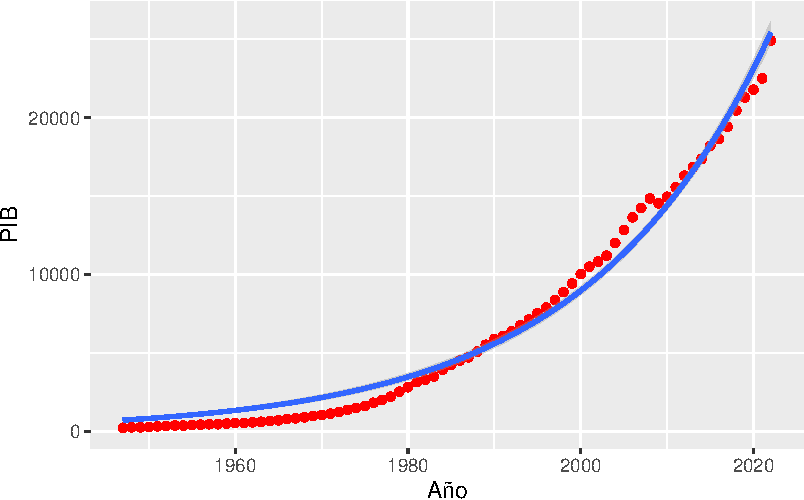
\includegraphics{05-regresion_files/figure-pdf/unnamed-chunk-29-1.pdf}

\begin{Shaded}
\begin{Highlighting}[]
        \FunctionTok{labs}\NormalTok{(}\AttributeTok{title =} \StringTok{"Evolución del PIB de Estados Unidos"}\NormalTok{, }\AttributeTok{x =} \StringTok{"Año"}\NormalTok{, }\AttributeTok{y =} \StringTok{"Logaritmo del PIB en billones dólares"}\NormalTok{)}
\end{Highlighting}
\end{Shaded}

\begin{verbatim}
$x
[1] "Año"

$y
[1] "Logaritmo del PIB en billones dólares"

$title
[1] "Evolución del PIB de Estados Unidos"

attr(,"class")
[1] "labels"
\end{verbatim}

  En este caso el ajuste no es perfecto, ya que es imposible que la
  recta pase por todos los puntos como ocurría en el ejercicio anterior.
  Por tanto, el ajuste es peor.

  \end{tcolorbox}
\item
  ¿Es el modelo de regresión exponencial un buen modelo para explicar la
  evolución del PIB?

  \begin{tcolorbox}[enhanced jigsaw, toprule=.15mm, rightrule=.15mm, arc=.35mm, colback=white, colbacktitle=quarto-callout-tip-color!10!white, toptitle=1mm, left=2mm, colframe=quarto-callout-tip-color-frame, opacityback=0, breakable, opacitybacktitle=0.6, bottomtitle=1mm, titlerule=0mm, title=\textcolor{quarto-callout-tip-color}{\faLightbulb}\hspace{0.5em}{Solución}, bottomrule=.15mm, coltitle=black, leftrule=.75mm]

\begin{Shaded}
\begin{Highlighting}[]
\FunctionTok{cat}\NormalTok{(}\FunctionTok{paste}\NormalTok{(}\StringTok{"Coeficiente de determinación exponencial R²:"}\NormalTok{, }\FunctionTok{summary}\NormalTok{(recta\_logPIB\_años)}\SpecialCharTok{$}\NormalTok{r.squared))}
\end{Highlighting}
\end{Shaded}

\begin{verbatim}
Coeficiente de determinación exponencial R²: 0.983487569858149
\end{verbatim}

  Como el coeficiente de determinación lineal vale 0.9834876 que está
  bastante próximo a 1, el ajuste es bueno, y el modelo exponencial
  explica muy bien la evolución del PIB.

  \end{tcolorbox}
\item
  Utilizar el modelo de regresión exponencial para predecir el PIB del
  año 2024. ¿Es fiable esta predicción?

  \begin{tcolorbox}[enhanced jigsaw, toprule=.15mm, rightrule=.15mm, arc=.35mm, colback=white, colbacktitle=quarto-callout-tip-color!10!white, toptitle=1mm, left=2mm, colframe=quarto-callout-tip-color-frame, opacityback=0, breakable, opacitybacktitle=0.6, bottomtitle=1mm, titlerule=0mm, title=\textcolor{quarto-callout-tip-color}{\faLightbulb}\hspace{0.5em}{Solución}, bottomrule=.15mm, coltitle=black, leftrule=.75mm]

\begin{Shaded}
\begin{Highlighting}[]
\CommentTok{\# El modelo exponencial devuelve el logaritmo del PIB, por lo que hay que aplicar la función exponencial para obtener el PIB.}
\FunctionTok{exp}\NormalTok{(}\FunctionTok{predict.lm}\NormalTok{(recta\_logPIB\_años, }\AttributeTok{newdata =} \FunctionTok{list}\NormalTok{(Año }\OtherTok{=} \DecValTok{2024}\NormalTok{)))}
\end{Highlighting}
\end{Shaded}

\begin{verbatim}
      1 
40486.8 
\end{verbatim}

  La predicción será fiable ya que el coeficiente de determinación está
  próximo a 1, el tamaño de la muestra no es muy pequeño y el año para
  el que se realiza la predicción no está lejos del rango de años de la
  muestra.

  \end{tcolorbox}
\item
  ¿Cuándo se alcanzará un PIB de 50000 billones de dólares?

  \begin{tcolorbox}[enhanced jigsaw, toprule=.15mm, rightrule=.15mm, arc=.35mm, colback=white, colbacktitle=quarto-callout-tip-color!10!white, toptitle=1mm, left=2mm, colframe=quarto-callout-tip-color-frame, opacityback=0, breakable, opacitybacktitle=0.6, bottomtitle=1mm, titlerule=0mm, title=\textcolor{quarto-callout-tip-color}{\faLightbulb}\hspace{0.5em}{Solución}, bottomrule=.15mm, coltitle=black, leftrule=.75mm]

  Como ahora queremos predecir el año en el que se alcanzará el PIB
  dado, necesitamos construir el modelo de regresión de los años sobre
  el PIB. Como la relación entre el PIB y los años es exponencial, la
  relación entre los años y el PIB será la inversa, es decir, el modelo
  logarítmico.

\begin{Shaded}
\begin{Highlighting}[]
\NormalTok{log\_años\_PIB }\OtherTok{\textless{}{-}} \FunctionTok{lm}\NormalTok{(Año }\SpecialCharTok{\textasciitilde{}} \FunctionTok{log}\NormalTok{(PIB), df) }
\FunctionTok{summary}\NormalTok{(log\_años\_PIB)}
\end{Highlighting}
\end{Shaded}

\begin{verbatim}

Call:
lm(formula = Año ~ log(PIB), data = df)

Residuals:
    Min      1Q  Median      3Q     Max 
-4.4049 -2.5367  0.2662  1.7718  6.4965 

Coefficients:
            Estimate Std. Error t value Pr(>|t|)    
(Intercept) 1863.498      1.852 1006.29   <2e-16 ***
log(PIB)      15.068      0.227   66.39   <2e-16 ***
---
Signif. codes:  0 '***' 0.001 '**' 0.01 '*' 0.05 '.' 0.1 ' ' 1

Residual standard error: 2.857 on 74 degrees of freedom
Multiple R-squared:  0.9835,    Adjusted R-squared:  0.9833 
F-statistic:  4407 on 1 and 74 DF,  p-value: < 2.2e-16
\end{verbatim}

  El modelo de regresión logarítmico de los años sobre el PIB es
  \(\textsf{Año}= 1863.4980331 + 15.0677514 \log(\textsf{PIB})\).

\begin{Shaded}
\begin{Highlighting}[]
\FunctionTok{predict.lm}\NormalTok{(log\_años\_PIB, }\AttributeTok{newdata =} \FunctionTok{list}\NormalTok{(}\AttributeTok{PIB =} \DecValTok{50000}\NormalTok{))}
\end{Highlighting}
\end{Shaded}

\begin{verbatim}
       1 
2026.528 
\end{verbatim}

  \end{tcolorbox}
\end{enumerate}

\end{exercise}

\begin{exercise}[]\protect\hypertarget{exr-regresion-5}{}\label{exr-regresion-5}

El fichero \href{datos/dieta.csv}{\texttt{dieta.csv}} contiene
información sobre el los kilos perdidos con una dieta de adelgazamiento.

\begin{enumerate}
\def\labelenumi{\alph{enumi}.}
\item
  Crear un data frame con los datos de la dieta a partir del fichero
  \href{https://aprendeconalf.es/estadistica-practicas-r/datos/dieta.csv}{\texttt{dieta.csv}}.

  \begin{tcolorbox}[enhanced jigsaw, toprule=.15mm, rightrule=.15mm, arc=.35mm, colback=white, colbacktitle=quarto-callout-tip-color!10!white, toptitle=1mm, left=2mm, colframe=quarto-callout-tip-color-frame, opacityback=0, breakable, opacitybacktitle=0.6, bottomtitle=1mm, titlerule=0mm, title=\textcolor{quarto-callout-tip-color}{\faLightbulb}\hspace{0.5em}{Solución}, bottomrule=.15mm, coltitle=black, leftrule=.75mm]

\begin{Shaded}
\begin{Highlighting}[]
\FunctionTok{library}\NormalTok{(readr)}
\NormalTok{df }\OtherTok{\textless{}{-}} \FunctionTok{read\_csv}\NormalTok{(}\StringTok{"https://aprendeconalf.es/estadistica{-}practicas{-}r/datos/dieta.csv"}\NormalTok{)}
\NormalTok{df}
\end{Highlighting}
\end{Shaded}

\begin{verbatim}
# A tibble: 40 x 3
    dias peso.perdido ejercicio
   <dbl>        <dbl> <chr>    
 1    14         2.95 no       
 2    18         5.65 no       
 3    22         6.56 no       
 4    26         3.56 no       
 5    30         6.17 no       
 6    34         9.4  no       
 7    38        12.4  no       
 8    42        12.9  no       
 9    46        13.9  no       
10    50        10.8  no       
# i 30 more rows
\end{verbatim}

  \end{tcolorbox}
\item
  Dibujar el diagrama de dispersión de los kilos perdidos en función del
  número de días con la dieta. ¿Qué tipo de modelo de regresión se
  ajusta mejor a la nube de puntos?

  \begin{tcolorbox}[enhanced jigsaw, toprule=.15mm, rightrule=.15mm, arc=.35mm, colback=white, colbacktitle=quarto-callout-tip-color!10!white, toptitle=1mm, left=2mm, colframe=quarto-callout-tip-color-frame, opacityback=0, breakable, opacitybacktitle=0.6, bottomtitle=1mm, titlerule=0mm, title=\textcolor{quarto-callout-tip-color}{\faLightbulb}\hspace{0.5em}{Solución}, bottomrule=.15mm, coltitle=black, leftrule=.75mm]

\begin{Shaded}
\begin{Highlighting}[]
\FunctionTok{library}\NormalTok{(ggplot2)}
\FunctionTok{ggplot}\NormalTok{(df, }\FunctionTok{aes}\NormalTok{(}\AttributeTok{x =}\NormalTok{ dias, }\AttributeTok{y =}\NormalTok{ peso.perdido)) }\SpecialCharTok{+}
    \FunctionTok{geom\_point}\NormalTok{(}\AttributeTok{col =} \StringTok{"red"}\NormalTok{) }\SpecialCharTok{+}
    \FunctionTok{labs}\NormalTok{(}\AttributeTok{title =} \StringTok{"Diagrama de dispersión del peso perdido y los días de dieta"}\NormalTok{, }\AttributeTok{x =} \StringTok{"Días de dieta"}\NormalTok{, }\AttributeTok{y =} \StringTok{"Peso perdido en Kg"}\NormalTok{)}
\end{Highlighting}
\end{Shaded}

  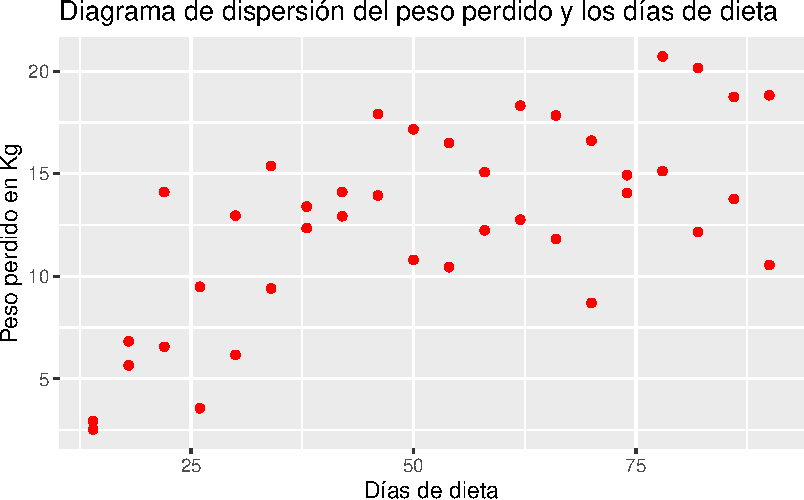
\includegraphics{05-regresion_files/figure-pdf/unnamed-chunk-35-1.pdf}

  La nube de puntos es bastante difusa aunque parece apreciarse una
  tendencia logarítmica o sigmoidal.

  \end{tcolorbox}
\item
  Calcular los coeficientes de determinación lineal, cuadrático,
  exponencial, logarítmico, potencial, inverso y sigmoidal. ¿Qué tipo de
  modelo explica mejor la relación entre los kilos perdidos y el número
  de días de dieta? ¿Qué porcentaje de la variabilidad de peso perdido
  explica el mejor modelo de regresión?

  \begin{tcolorbox}[enhanced jigsaw, toprule=.15mm, rightrule=.15mm, arc=.35mm, colback=white, colbacktitle=quarto-callout-tip-color!10!white, toptitle=1mm, left=2mm, colframe=quarto-callout-tip-color-frame, opacityback=0, breakable, opacitybacktitle=0.6, bottomtitle=1mm, titlerule=0mm, title=\textcolor{quarto-callout-tip-color}{\faLightbulb}\hspace{0.5em}{Solución}, bottomrule=.15mm, coltitle=black, leftrule=.75mm]

\begin{Shaded}
\begin{Highlighting}[]
\FunctionTok{library}\NormalTok{(dplyr)}
\FunctionTok{library}\NormalTok{(tidyr)}
\FunctionTok{library}\NormalTok{(purrr)}
\FunctionTok{library}\NormalTok{(broom)}
\FunctionTok{library}\NormalTok{(kableExtra)}
\CommentTok{\# Construimos un data frame con el ajuste de los modelos.}
\NormalTok{modelos }\OtherTok{\textless{}{-}} \FunctionTok{tibble}\NormalTok{(}
        \AttributeTok{Lineal =} \FunctionTok{list}\NormalTok{(}\FunctionTok{lm}\NormalTok{(peso.perdido }\SpecialCharTok{\textasciitilde{}}\NormalTok{ dias, df)),}
        \AttributeTok{Cuadratico =} \FunctionTok{list}\NormalTok{(}\FunctionTok{lm}\NormalTok{(peso.perdido }\SpecialCharTok{\textasciitilde{}}\NormalTok{ dias }\SpecialCharTok{+} \FunctionTok{I}\NormalTok{(dias}\SpecialCharTok{\^{}}\DecValTok{2}\NormalTok{), df)),}
        \AttributeTok{Exponencial =} \FunctionTok{list}\NormalTok{(}\FunctionTok{lm}\NormalTok{(}\FunctionTok{log}\NormalTok{(peso.perdido) }\SpecialCharTok{\textasciitilde{}}\NormalTok{ dias, df)),}
        \AttributeTok{Logaritmico =} \FunctionTok{list}\NormalTok{(}\FunctionTok{lm}\NormalTok{(peso.perdido }\SpecialCharTok{\textasciitilde{}} \FunctionTok{log}\NormalTok{(dias), df)),}
        \AttributeTok{Potencial =} \FunctionTok{list}\NormalTok{(}\FunctionTok{lm}\NormalTok{(}\FunctionTok{log}\NormalTok{(peso.perdido) }\SpecialCharTok{\textasciitilde{}} \FunctionTok{log}\NormalTok{(dias), df)),}
        \AttributeTok{Inverso =} \FunctionTok{list}\NormalTok{(}\FunctionTok{lm}\NormalTok{(peso.perdido }\SpecialCharTok{\textasciitilde{}} \FunctionTok{I}\NormalTok{(}\DecValTok{1}\SpecialCharTok{/}\NormalTok{dias), df)),}
        \AttributeTok{Sigmoidal =} \FunctionTok{list}\NormalTok{(}\FunctionTok{lm}\NormalTok{(}\FunctionTok{log}\NormalTok{(peso.perdido) }\SpecialCharTok{\textasciitilde{}} \FunctionTok{I}\NormalTok{(}\DecValTok{1}\SpecialCharTok{/}\NormalTok{dias), df)),}
\NormalTok{    )  }\SpecialCharTok{|\textgreater{}} 
    \CommentTok{\# }
    \CommentTok{\# Reestructuramos el data frame para tener todos los modelos en la misma columna.}
    \FunctionTok{pivot\_longer}\NormalTok{(}\FunctionTok{everything}\NormalTok{(), }\AttributeTok{names\_to =} \StringTok{"Tipo\_Modelo"}\NormalTok{, }\AttributeTok{values\_to =} \StringTok{"Modelo"}\NormalTok{)  }\SpecialCharTok{|\textgreater{}} 
    \CommentTok{\# Obtenemos un resumen del ajuste de cada modelo en formato organizado (se obtiene una lista con los parámetros que describen el ajuste de cada modelo).}
    \FunctionTok{mutate}\NormalTok{(}\AttributeTok{Resumen =} \FunctionTok{map}\NormalTok{(Modelo, glance)) }\SpecialCharTok{|\textgreater{}} 
    \CommentTok{\# Desanidamos el resumen (se obtiene una columna para cada parámetro del resumen del ajuste de los modelos).}
    \FunctionTok{unnest}\NormalTok{(Resumen)  }\SpecialCharTok{|\textgreater{}} 
    \CommentTok{\# Ordenamos el data frame por el coeficiente de determinación.}
    \FunctionTok{arrange}\NormalTok{(}\SpecialCharTok{{-}}\NormalTok{r.squared)}

\NormalTok{modelos  }\SpecialCharTok{|\textgreater{}}
    \FunctionTok{select}\NormalTok{(Tipo\_Modelo, r.squared)  }\SpecialCharTok{|\textgreater{}} 
    \FunctionTok{kable}\NormalTok{(}\AttributeTok{col.names =} \FunctionTok{c}\NormalTok{(}\StringTok{"Tipo de Modelo"}\NormalTok{, }\StringTok{"R²"}\NormalTok{)) }\SpecialCharTok{|\textgreater{}}
    \FunctionTok{kable\_styling}\NormalTok{(}\AttributeTok{full\_width =}\NormalTok{ F)}
\end{Highlighting}
\end{Shaded}

  \begin{table}
  \centering
  \begin{tabular}{l|r}
  \hline
  Tipo de Modelo & R²\\
  \hline
  Sigmoidal & 0.6662170\\
  \hline
  Potencial & 0.5684490\\
  \hline
  Inverso & 0.5583853\\
  \hline
  Cuadratico & 0.5397848\\
  \hline
  Logaritmico & 0.5254856\\
  \hline
  Lineal & 0.4356390\\
  \hline
  Exponencial & 0.4308936\\
  \hline
  \end{tabular}
  \end{table}

  El mejor modelo es el Sigmoidal que explica el 66.6216965388749\% de
  la variabilidad del peso perdido.

  \end{tcolorbox}
\item
  Dibujar el diagrama de dispersión de los kilos perdidos en función del
  número de días con la dieta según si la persona hace ejercicio o no.
  ¿Qué conclusiones se pueden sacar?

  \begin{tcolorbox}[enhanced jigsaw, toprule=.15mm, rightrule=.15mm, arc=.35mm, colback=white, colbacktitle=quarto-callout-tip-color!10!white, toptitle=1mm, left=2mm, colframe=quarto-callout-tip-color-frame, opacityback=0, breakable, opacitybacktitle=0.6, bottomtitle=1mm, titlerule=0mm, title=\textcolor{quarto-callout-tip-color}{\faLightbulb}\hspace{0.5em}{Solución}, bottomrule=.15mm, coltitle=black, leftrule=.75mm]

\begin{Shaded}
\begin{Highlighting}[]
\FunctionTok{library}\NormalTok{(ggplot2)}
\FunctionTok{ggplot}\NormalTok{(df, }\FunctionTok{aes}\NormalTok{(}\AttributeTok{x =}\NormalTok{ dias, }\AttributeTok{y =}\NormalTok{ peso.perdido, }\AttributeTok{color =}\NormalTok{ ejercicio)) }\SpecialCharTok{+}
    \FunctionTok{geom\_point}\NormalTok{() }\SpecialCharTok{+}
    \FunctionTok{labs}\NormalTok{(}\AttributeTok{title =} \StringTok{"Diagrama de dispersión del peso perdido y los días de dieta"}\NormalTok{, }\AttributeTok{x =} \StringTok{"Días de dieta"}\NormalTok{, }\AttributeTok{y =} \StringTok{"Peso perdido en Kg"}\NormalTok{)}
\end{Highlighting}
\end{Shaded}

  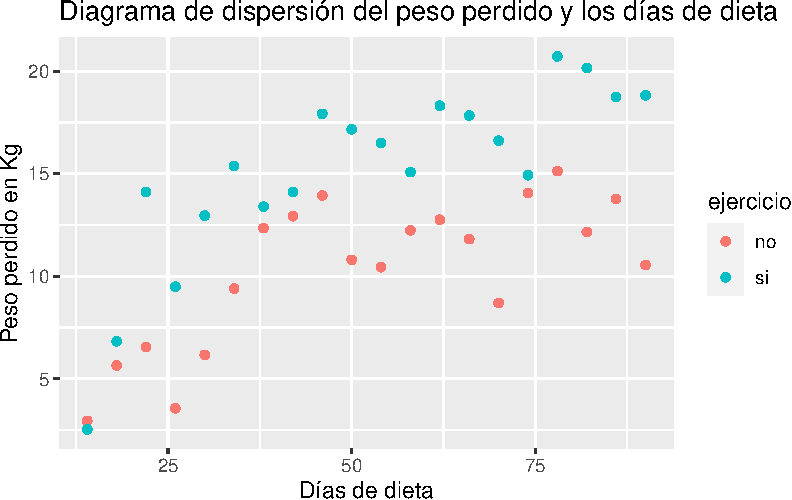
\includegraphics{05-regresion_files/figure-pdf/unnamed-chunk-37-1.pdf}

  Claramente la nube de puntos de las personas que hacen ejercicio está
  por encima de la de los que no hacen ejercicio, lo que indica que
  hacer ejercicio favorece la pérdida de peso. Los más razonable es
  construir modelos de regresión para cada grupo.

  \end{tcolorbox}
\item
  ¿Qué tipo de modelo explica mejor la relación entre el peso perdido y
  los días de dieta en el grupo de las personas que hacen ejercicio? ¿Y
  en el grupo de las que no hacen ejercicio? ¿Han mejorado los modelos
  con respecto al modelo anterior?

  \begin{tcolorbox}[enhanced jigsaw, toprule=.15mm, rightrule=.15mm, arc=.35mm, colback=white, colbacktitle=quarto-callout-tip-color!10!white, toptitle=1mm, left=2mm, colframe=quarto-callout-tip-color-frame, opacityback=0, breakable, opacitybacktitle=0.6, bottomtitle=1mm, titlerule=0mm, title=\textcolor{quarto-callout-tip-color}{\faLightbulb}\hspace{0.5em}{Solución}, bottomrule=.15mm, coltitle=black, leftrule=.75mm]

\begin{Shaded}
\begin{Highlighting}[]
\NormalTok{modelos }\OtherTok{\textless{}{-}}\NormalTok{ df  }\SpecialCharTok{|\textgreater{}} 
    \CommentTok{\# Anidamos por la columna ejercicio.}
    \FunctionTok{nest\_by}\NormalTok{(ejercicio)  }\SpecialCharTok{|\textgreater{}} 
    \CommentTok{\# Ajustamos los modelos de regresión.}
    \FunctionTok{mutate}\NormalTok{(}
        \AttributeTok{Lineal =} \FunctionTok{list}\NormalTok{(}\FunctionTok{lm}\NormalTok{(peso.perdido }\SpecialCharTok{\textasciitilde{}}\NormalTok{ dias, data)),}
        \AttributeTok{Cuadratico =} \FunctionTok{list}\NormalTok{(}\FunctionTok{lm}\NormalTok{(peso.perdido }\SpecialCharTok{\textasciitilde{}}\NormalTok{ dias }\SpecialCharTok{+} \FunctionTok{I}\NormalTok{(dias}\SpecialCharTok{\^{}}\DecValTok{2}\NormalTok{), data)),}
        \AttributeTok{Exponencial =} \FunctionTok{list}\NormalTok{(}\FunctionTok{lm}\NormalTok{(}\FunctionTok{log}\NormalTok{(peso.perdido) }\SpecialCharTok{\textasciitilde{}}\NormalTok{ dias, data)),}
        \AttributeTok{Logaritmico =} \FunctionTok{list}\NormalTok{(}\FunctionTok{lm}\NormalTok{(peso.perdido }\SpecialCharTok{\textasciitilde{}} \FunctionTok{log}\NormalTok{(dias), data)),}
        \AttributeTok{Potencial =} \FunctionTok{list}\NormalTok{(}\FunctionTok{lm}\NormalTok{(}\FunctionTok{log}\NormalTok{(peso.perdido) }\SpecialCharTok{\textasciitilde{}} \FunctionTok{log}\NormalTok{(dias), data)),}
        \AttributeTok{Inverso =} \FunctionTok{list}\NormalTok{(}\FunctionTok{lm}\NormalTok{(peso.perdido }\SpecialCharTok{\textasciitilde{}} \FunctionTok{I}\NormalTok{(}\DecValTok{1}\SpecialCharTok{/}\NormalTok{dias), data)),}
        \AttributeTok{Sigmoidal =} \FunctionTok{list}\NormalTok{(}\FunctionTok{lm}\NormalTok{(}\FunctionTok{log}\NormalTok{(peso.perdido) }\SpecialCharTok{\textasciitilde{}} \FunctionTok{I}\NormalTok{(}\DecValTok{1}\SpecialCharTok{/}\NormalTok{dias), data)),}
\NormalTok{    )  }\SpecialCharTok{|\textgreater{}} 
    \CommentTok{\# Reestructuramos el data frame para tener todos los modelos en la misma columna.}
    \FunctionTok{pivot\_longer}\NormalTok{(}\SpecialCharTok{{-}}\FunctionTok{c}\NormalTok{(ejercicio, data), }\AttributeTok{names\_to =} \StringTok{"Tipo\_Modelo"}\NormalTok{, }\AttributeTok{values\_to =} \StringTok{"Modelo"}\NormalTok{)  }\SpecialCharTok{|\textgreater{}} 
    \CommentTok{\# Obtenemos un resumen del ajuste de cada modelo en formato organizado (se obtiene una lista con los parámetros que describen el ajuste de cada modelo).}
    \FunctionTok{mutate}\NormalTok{(}\AttributeTok{Resumen =} \FunctionTok{map}\NormalTok{(Modelo, glance)) }\SpecialCharTok{|\textgreater{}} 
    \CommentTok{\# Desanidamos el resumen (se obtiene una columna para cada parámetro del resumen del ajuste de los modelos).}
    \FunctionTok{unnest}\NormalTok{(Resumen)  }\SpecialCharTok{|\textgreater{}} 
    \CommentTok{\# Ordenamos el data frame por la columna ejercicio y por el coeficiente de determinación.}
    \FunctionTok{arrange}\NormalTok{(ejercicio, }\SpecialCharTok{{-}}\NormalTok{r.squared)  }
\NormalTok{modelos }\SpecialCharTok{|\textgreater{}} 
    \FunctionTok{select}\NormalTok{(ejercicio, Tipo\_Modelo, r.squared)  }\SpecialCharTok{|\textgreater{}} 
    \FunctionTok{kable}\NormalTok{(}\AttributeTok{col.names =} \FunctionTok{c}\NormalTok{(}\StringTok{"Ejercicio"}\NormalTok{, }\StringTok{"Tipo de Modelo"}\NormalTok{, }\StringTok{"R²"}\NormalTok{)) }\SpecialCharTok{|\textgreater{}}
    \FunctionTok{pack\_rows}\NormalTok{(}\AttributeTok{index =} \FunctionTok{table}\NormalTok{(modelos}\SpecialCharTok{$}\NormalTok{ejercicio))  }\SpecialCharTok{|\textgreater{}} 
    \FunctionTok{kable\_styling}\NormalTok{(}\AttributeTok{full\_width =}\NormalTok{ F)}
\end{Highlighting}
\end{Shaded}

  \begin{table}
  \centering
  \begin{tabular}{l|l|r}
  \hline
  Ejercicio & Tipo de Modelo & R²\\
  \hline
  \multicolumn{3}{l}{\textbf{no}}\\
  \hline
  \hspace{1em}no & Sigmoidal & 0.7401212\\
  \hline
  \hspace{1em}no & Cuadratico & 0.7100610\\
  \hline
  \hspace{1em}no & Inverso & 0.6796880\\
  \hline
  \hspace{1em}no & Potencial & 0.6700051\\
  \hline
  \hspace{1em}no & Logaritmico & 0.6494521\\
  \hline
  \hspace{1em}no & Lineal & 0.5286338\\
  \hline
  \hspace{1em}no & Exponencial & 0.5222832\\
  \hline
  \multicolumn{3}{l}{\textbf{si}}\\
  \hline
  \hspace{1em}si & Inverso & 0.8470993\\
  \hline
  \hspace{1em}si & Sigmoidal & 0.8305013\\
  \hline
  \hspace{1em}si & Logaritmico & 0.7885173\\
  \hline
  \hspace{1em}si & Cuadratico & 0.7791671\\
  \hline
  \hspace{1em}si & Potencial & 0.6704843\\
  \hline
  \hspace{1em}si & Lineal & 0.6623502\\
  \hline
  \hspace{1em}si & Exponencial & 0.4945564\\
  \hline
  \end{tabular}
  \end{table}

  El mejor modelo en el grupo de los que hacen ejercicio es el inverso y
  en el grupo de los que no el sigmoidal. Los modelos han mejorado
  bastante con respecto al modelo anterior, sobre todo el del grupo de
  personas que hace ejercicio.

  \end{tcolorbox}
\item
  Construir el mejor modelo de regresión del peso perdido sobre los días
  de dieta para el grupo de las personas que hacen ejercicio y para el
  grupo de las que no.

  \begin{tcolorbox}[enhanced jigsaw, toprule=.15mm, rightrule=.15mm, arc=.35mm, colback=white, colbacktitle=quarto-callout-tip-color!10!white, toptitle=1mm, left=2mm, colframe=quarto-callout-tip-color-frame, opacityback=0, breakable, opacitybacktitle=0.6, bottomtitle=1mm, titlerule=0mm, title=\textcolor{quarto-callout-tip-color}{\faLightbulb}\hspace{0.5em}{Solución}, bottomrule=.15mm, coltitle=black, leftrule=.75mm]

  Construimos el modelo inverso para el grupo de las personas que hacen
  ejercicio.

\begin{Shaded}
\begin{Highlighting}[]
\NormalTok{inverso\_ejercicio }\OtherTok{\textless{}{-}} \FunctionTok{lm}\NormalTok{(peso.perdido }\SpecialCharTok{\textasciitilde{}} \FunctionTok{I}\NormalTok{(}\DecValTok{1}\SpecialCharTok{/}\NormalTok{dias), df[df}\SpecialCharTok{$}\NormalTok{ejercicio }\SpecialCharTok{==} \StringTok{"si"}\NormalTok{, ])}
\FunctionTok{summary}\NormalTok{(inverso\_ejercicio)}
\end{Highlighting}
\end{Shaded}

\begin{verbatim}

Call:
lm(formula = peso.perdido ~ I(1/dias), data = df[df$ejercicio == 
    "si", ])

Residuals:
    Min      1Q  Median      3Q     Max 
-3.1866 -1.3268  0.0011  0.9810  4.1456 

Coefficients:
             Estimate Std. Error t value Pr(>|t|)    
(Intercept)   21.5655     0.7653  28.181 2.42e-16 ***
I(1/dias)   -255.2249    25.5579  -9.986 9.12e-09 ***
---
Signif. codes:  0 '***' 0.001 '**' 0.01 '*' 0.05 '.' 0.1 ' ' 1

Residual standard error: 1.811 on 18 degrees of freedom
Multiple R-squared:  0.8471,    Adjusted R-squared:  0.8386 
F-statistic: 99.72 on 1 and 18 DF,  p-value: 9.123e-09
\end{verbatim}

  Y ahora el modelo sigmoidal para el grupo de las personas que no hacen
  ejercicio.

\begin{Shaded}
\begin{Highlighting}[]
\NormalTok{sigmoidal\_no\_ejercicio }\OtherTok{\textless{}{-}} \FunctionTok{lm}\NormalTok{(}\FunctionTok{log}\NormalTok{(peso.perdido) }\SpecialCharTok{\textasciitilde{}} \FunctionTok{I}\NormalTok{(}\DecValTok{1}\SpecialCharTok{/}\NormalTok{dias), df[df}\SpecialCharTok{$}\NormalTok{ejercicio }\SpecialCharTok{==} \StringTok{"no"}\NormalTok{, ])}
\FunctionTok{summary}\NormalTok{(sigmoidal\_no\_ejercicio)}
\end{Highlighting}
\end{Shaded}

\begin{verbatim}

Call:
lm(formula = log(peso.perdido) ~ I(1/dias), data = df[df$ejercicio == 
    "no", ])

Residuals:
     Min       1Q   Median       3Q      Max 
-0.66026 -0.07192  0.04678  0.13142  0.29633 

Coefficients:
            Estimate Std. Error t value Pr(>|t|)    
(Intercept)   2.8694     0.1021   28.09 2.55e-16 ***
I(1/dias)   -24.4226     3.4111   -7.16 1.15e-06 ***
---
Signif. codes:  0 '***' 0.001 '**' 0.01 '*' 0.05 '.' 0.1 ' ' 1

Residual standard error: 0.2417 on 18 degrees of freedom
Multiple R-squared:  0.7401,    Adjusted R-squared:  0.7257 
F-statistic: 51.26 on 1 and 18 DF,  p-value: 1.146e-06
\end{verbatim}

  \end{tcolorbox}
\item
  Según los mejores modelos de regresión en cada caso, ¿cuántos kilos
  perderá una persona que hace ejercicio tras 100 días de dieta? ¿Y una
  que no hace ejercicio?

  \begin{tcolorbox}[enhanced jigsaw, toprule=.15mm, rightrule=.15mm, arc=.35mm, colback=white, colbacktitle=quarto-callout-tip-color!10!white, toptitle=1mm, left=2mm, colframe=quarto-callout-tip-color-frame, opacityback=0, breakable, opacitybacktitle=0.6, bottomtitle=1mm, titlerule=0mm, title=\textcolor{quarto-callout-tip-color}{\faLightbulb}\hspace{0.5em}{Solución}, bottomrule=.15mm, coltitle=black, leftrule=.75mm]

  Hacemos primero la predicción del peso perdido para la persona que
  hace ejercicio usando el modelo inverso.

\begin{Shaded}
\begin{Highlighting}[]
\FunctionTok{predict.lm}\NormalTok{(inverso\_ejercicio, }\AttributeTok{newdata =} \FunctionTok{list}\NormalTok{(}\AttributeTok{dias =} \DecValTok{100}\NormalTok{))}
\end{Highlighting}
\end{Shaded}

\begin{verbatim}
       1 
19.01329 
\end{verbatim}

  Y ahora hacemos la predicción del peso perdido para la persona que no
  hace ejercicio usando el modelo sigmoidal.

\begin{Shaded}
\begin{Highlighting}[]
\CommentTok{\# El modelo sigmoidal devuelve el logaritmo del peso perdido por lo que hay que aplicar la función exponencial para obtener el peso perdido.}
\FunctionTok{exp}\NormalTok{(}\FunctionTok{predict.lm}\NormalTok{(sigmoidal\_no\_ejercicio, }\AttributeTok{newdata =} \FunctionTok{list}\NormalTok{(}\AttributeTok{dias =} \DecValTok{100}\NormalTok{)))}
\end{Highlighting}
\end{Shaded}

\begin{verbatim}
       1 
13.80634 
\end{verbatim}

  \end{tcolorbox}
\end{enumerate}

\end{exercise}

\section{Ejercicios propuestos}\label{ejercicios-propuestos-3}

\begin{exercise}[]\protect\hypertarget{exr-regresion-6}{}\label{exr-regresion-6}

El conjunto de datos
\href{https://aprendeconalf.es/estadistica-practicas-r/datos/neonatos.csv}{\texttt{neonatos}}
contiene información sobre una muestra de 320 recién nacidos en un
hospital durante un año que cumplieron el tiempo normal de gestación.

\begin{enumerate}
\def\labelenumi{\alph{enumi}.}
\item
  Crear un data frame a con los datos de los neonatos a partir del
  fichero anterior.
\item
  Construir la recta de regresión del peso de los recién nacidos sobre
  el número de cigarros fumados al día por las madres. ¿Existe una
  relación lineal fuerte entre el peso y el número de cigarros?
\item
  Dibujar la recta de regresión calculada en el apartado anterior. ¿Por
  qué la recta no se ajusta bien a la nube de puntos?
\item
  Calcular y dibujar la recta de regresión del peso de los recién
  nacidos sobre el número de cigarros fumados al día por las madres en
  el grupo de las madres que si fumaron durante el embarazo. ¿Es este
  modelo mejor o pero que la recta del apartado anterior?
\item
  Según este modelo, ¿cuánto disminuirá el peso del recién nacido por
  cada cigarro más diario que fume la madre?
\item
  Según el modelo anterior, ¿qué peso tendrá un recién nacido de una
  madre que ha fumado 5 cigarros diarios durante el embarazo? ¿Y si la
  madre ha fumado 30 cigarros diarios durante el embarazo? ¿Son fiables
  estas predicciones?
\item
  ¿Existe la misma relación lineal entre el peso de los recién nacidos y
  el número de cigarros fumados al día por las madres que fumaron
  durante el embarazo en el grupo de las madres menores de 20 y en el
  grupo de las madres mayores de 20? ¿Qué se puede concluir?
\end{enumerate}

\end{exercise}

\begin{exercise}[]\protect\hypertarget{exr-regresion-7}{}\label{exr-regresion-7}

El conjunto de datos
\href{https://aprendeconalf.es/estadistica-practicas-r/datos/edad-estatura.csv}{\texttt{edad.estatura}}
contiene la edad y la estatura de 30 personas.

\begin{enumerate}
\def\labelenumi{\alph{enumi}.}
\item
  Crear un data frame con los datos de las edades y las estaturas a
  partir del fichero anterior.
\item
  Calcular la recta de regresión de la estatura sobre la edad. ¿Es un
  buen modelo la recta de regresión?
\item
  Dibujar el diagrama de dispersión de la estatura sobre la edad.
  ¿Alrededor de qué edad se observa un cambio en la tendencia?
\item
  Recodificar la variable edad en dos grupos para mayores y menores de
  20 años.
\item
  Calcular la recta de regresión de la estatura sobre la edad para cada
  grupo de edad. ¿En qué grupo explica mejor la recta de regresión la
  relación entre la estatura y la edad?
\item
  Dibujar las rectas de regresión anteriores.
\item
  ¿Qué estatura se espera que tenga una persona de 14 años? ¿Y una de
  38?
\end{enumerate}

\end{exercise}

\begin{exercise}[]\protect\hypertarget{exr-regresion-8}{}\label{exr-regresion-8}

El conjunto de datos \texttt{gapminder} del paquete \texttt{gapminder}
contiene información sobre la esperanza de vida, la población, y el PIB
per cápita en dólares PPP de los principales países en un rango de años.

\begin{enumerate}
\def\labelenumi{\alph{enumi}.}
\item
  Instalar el paquete \texttt{gapminder} y cargarlo.
\item
  ¿Qué tipo de modelo explica mejor la evolución de la población con los
  años? Construir ese modelo.
\item
  ¿Qué tipo de modelo explica mejor la relación entre la esperanza de
  vida y el PIB per cápita?
\item
  ¿Qué tipo de modelo explica mejor la relación entre la esperanza de
  vida y el PIB r cápita para cada continente? Construir el mejor modelo
  en cada caso y utilizarlo para predecir la esperanza de vida de una
  persona de cada continente con un PIB per cápita de 1000 dólares PPP.
\end{enumerate}

\end{exercise}

\bookmarksetup{startatroot}

\chapter{Distribuciones de
probabilidad}\label{distribuciones-de-probabilidad}

\section{Ejercicios Resueltos}\label{ejercicios-resueltos-4}

Para la realización de esta práctica se requieren los siguientes
paquetes:

\begin{Shaded}
\begin{Highlighting}[]
\FunctionTok{library}\NormalTok{(tidyverse) }
\CommentTok{\# Incluye los siguientes paquetes:}
\CommentTok{\# {-} dplyr: para el preprocesamiento y manipulación de datos.}
\CommentTok{\# {-} ggplot2: para la representación gráfica.}
\CommentTok{\# {-} purrr: para aplicar funciones a vectores. }
\FunctionTok{library}\NormalTok{(extraDistr) }\CommentTok{\# para distribuciones de probabilidad adicionales.}
\FunctionTok{library}\NormalTok{(knitr) }\CommentTok{\# para el formateo de tablas.}
\FunctionTok{library}\NormalTok{(kableExtra) }\CommentTok{\# para personalizar el formato de las tablas.}
\end{Highlighting}
\end{Shaded}

\begin{exercise}[]\protect\hypertarget{exr-distribuciones-probabilidad-1}{}\label{exr-distribuciones-probabilidad-1}

Sea \(X\) la variable que mide el resultado obtenido al lanzar un dado.

\begin{enumerate}
\def\labelenumi{\alph{enumi}.}
\item
  ¿Qué tipo de modelo de distribución de probabilidad sigue \(X\)?
  Construir su función de probabilidad.

  \begin{tcolorbox}[enhanced jigsaw, toprule=.15mm, rightrule=.15mm, arc=.35mm, colback=white, colbacktitle=quarto-callout-tip-color!10!white, toptitle=1mm, left=2mm, colframe=quarto-callout-tip-color-frame, opacityback=0, breakable, opacitybacktitle=0.6, bottomtitle=1mm, titlerule=0mm, title=\textcolor{quarto-callout-tip-color}{\faLightbulb}\hspace{0.5em}{Solución}, bottomrule=.15mm, coltitle=black, leftrule=.75mm]

  Se trata de una
  \href{https://es.wikipedia.org/wiki/Distribuci\%C3\%B3n_uniforme_discreta}{distribución
  uniforme discreta} \(U(1, 6)\). Para calcular probabilidades con el
  modelo uniforme discreto se utiliza la función
  \href{https://www.rdocumentation.org/packages/extraDistr/versions/1.9.1/topics/DiscreteUniform}{\texttt{ddunif(x,\ min,\ max)}}
  del paquete \texttt{extraDistr}, donde \texttt{min} es el mínimo valor
  que puede tomar la variable, \texttt{max} es el máximo valor que puede
  tomar la variable y \texttt{x} es el valor de la variable.

\begin{Shaded}
\begin{Highlighting}[]
\FunctionTok{library}\NormalTok{(extraDistr)}
\FunctionTok{library}\NormalTok{(kableExtra)}
\NormalTok{x }\OtherTok{\textless{}{-}} \DecValTok{1}\SpecialCharTok{:}\DecValTok{6}
\NormalTok{f }\OtherTok{\textless{}{-}} \FunctionTok{ddunif}\NormalTok{(x, }\DecValTok{1}\NormalTok{, }\DecValTok{6}\NormalTok{)}
\NormalTok{df }\OtherTok{\textless{}{-}} \FunctionTok{data.frame}\NormalTok{(x, f)}
\NormalTok{df }\SpecialCharTok{|\textgreater{}} 
    \FunctionTok{kable}\NormalTok{() }\SpecialCharTok{|\textgreater{}} 
    \FunctionTok{kable\_styling}\NormalTok{(}\AttributeTok{full\_width =}\NormalTok{ F)}
\end{Highlighting}
\end{Shaded}

  \begin{table}
  \centering
  \begin{tabular}{r|r}
  \hline
  x & f\\
  \hline
  1 & 0.1666667\\
  \hline
  2 & 0.1666667\\
  \hline
  3 & 0.1666667\\
  \hline
  4 & 0.1666667\\
  \hline
  5 & 0.1666667\\
  \hline
  6 & 0.1666667\\
  \hline
  \end{tabular}
  \end{table}

  \end{tcolorbox}
\item
  Dibujar la gráfica de la función de probabilidad del modelo de
  probabilidad anterior.

  \begin{tcolorbox}[enhanced jigsaw, toprule=.15mm, rightrule=.15mm, arc=.35mm, colback=white, colbacktitle=quarto-callout-tip-color!10!white, toptitle=1mm, left=2mm, colframe=quarto-callout-tip-color-frame, opacityback=0, breakable, opacitybacktitle=0.6, bottomtitle=1mm, titlerule=0mm, title=\textcolor{quarto-callout-tip-color}{\faLightbulb}\hspace{0.5em}{Solución}, bottomrule=.15mm, coltitle=black, leftrule=.75mm]

\begin{Shaded}
\begin{Highlighting}[]
\FunctionTok{library}\NormalTok{(ggplot2)}
\FunctionTok{ggplot}\NormalTok{(df, }\FunctionTok{aes}\NormalTok{(}\AttributeTok{x =}\NormalTok{ x, }\AttributeTok{y =}\NormalTok{ f)) }\SpecialCharTok{+}
    \FunctionTok{geom\_point}\NormalTok{(}\AttributeTok{color =} \StringTok{"steelblue"}\NormalTok{) }\SpecialCharTok{+}
    \FunctionTok{labs}\NormalTok{(}\AttributeTok{title =} \StringTok{"Función de probabilidad uniforme U(1,6)"}\NormalTok{, }\AttributeTok{x =} \StringTok{"Número obtenido"}\NormalTok{, }\AttributeTok{y =} \StringTok{"Probabilidad"}\NormalTok{)}
\end{Highlighting}
\end{Shaded}

  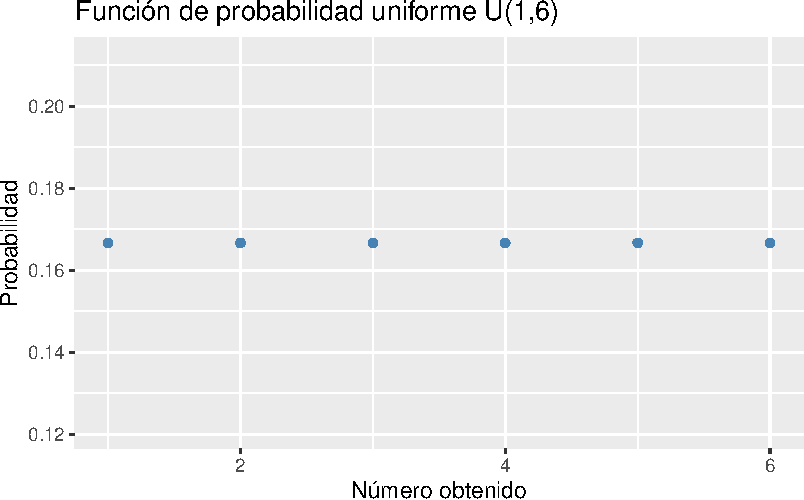
\includegraphics{06-distribuciones-probabilidad_files/figure-pdf/unnamed-chunk-2-1.pdf}

  \end{tcolorbox}
\item
  Simular el experimento aleatorio del lanzamiento de un dado. Repetir
  el lanzamiento un millón de veces y dibujar el diagrama de barras de
  la distribución de frecuencias resultante. ¿Se parece a la
  distribución de probabilidad anterior?

  \begin{tcolorbox}[enhanced jigsaw, toprule=.15mm, rightrule=.15mm, arc=.35mm, colback=white, colbacktitle=quarto-callout-tip-color!10!white, toptitle=1mm, left=2mm, colframe=quarto-callout-tip-color-frame, opacityback=0, breakable, opacitybacktitle=0.6, bottomtitle=1mm, titlerule=0mm, title=\textcolor{quarto-callout-tip-color}{\faLightbulb}\hspace{0.5em}{Solución}, bottomrule=.15mm, coltitle=black, leftrule=.75mm]

\begin{Shaded}
\begin{Highlighting}[]
\CommentTok{\# Fijamos una semilla de aleatorización para obtener resultados reproducibles.}
\FunctionTok{set.seed}\NormalTok{(}\DecValTok{123}\NormalTok{)}
\FunctionTok{data.frame}\NormalTok{(}\AttributeTok{x =} \FunctionTok{rdunif}\NormalTok{(}\DecValTok{10}\SpecialCharTok{\^{}}\DecValTok{6}\NormalTok{, }\DecValTok{1}\NormalTok{, }\DecValTok{6}\NormalTok{))  }\SpecialCharTok{|\textgreater{}} 
    \FunctionTok{ggplot}\NormalTok{(}\FunctionTok{aes}\NormalTok{(}\AttributeTok{x =}\NormalTok{ x)) }\SpecialCharTok{+}
    \FunctionTok{geom\_bar}\NormalTok{(}\FunctionTok{aes}\NormalTok{(}\AttributeTok{y =} \FunctionTok{after\_stat}\NormalTok{(count}\SpecialCharTok{/}\FunctionTok{sum}\NormalTok{(count))), }\AttributeTok{fill =} \StringTok{"steelblue"}\NormalTok{) }\SpecialCharTok{+}
    \FunctionTok{labs}\NormalTok{(}\AttributeTok{title =} \StringTok{"Distribución de frecuencias del lanzamiento de un dado"}\NormalTok{, }\AttributeTok{x =} \StringTok{"Número obtenido"}\NormalTok{, }\AttributeTok{y =} \StringTok{"Frecuencia relativa"}\NormalTok{)}
\end{Highlighting}
\end{Shaded}

  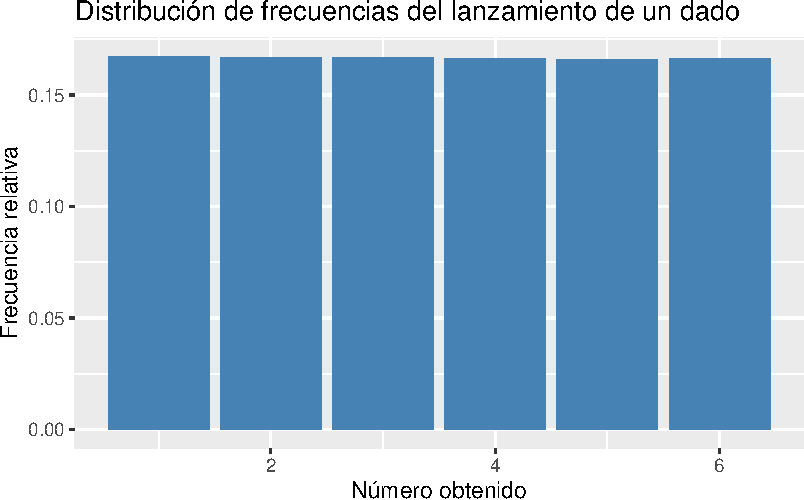
\includegraphics{06-distribuciones-probabilidad_files/figure-pdf/unnamed-chunk-3-1.pdf}

  La distribución experimental obtenida es casi idéntica a la
  distribución teórica del modelo uniforme \(U(1,6)\).

  \end{tcolorbox}
\end{enumerate}

\end{exercise}

\begin{exercise}[]\protect\hypertarget{exr-distribuciones-probabilidad-2}{}\label{exr-distribuciones-probabilidad-2}

Un test consta de 10 preguntas de opción múltiple con cuatro posibles
respuestas para cada pregunta.

\begin{enumerate}
\def\labelenumi{\alph{enumi}.}
\item
  ¿Qué tipo de modelo de distribución de probabilidad sigue la variable
  que mide el número de aciertos al responder todas las preguntas
  aleatoriamente? Construir su función de probabilidad.

  \begin{tcolorbox}[enhanced jigsaw, toprule=.15mm, rightrule=.15mm, arc=.35mm, colback=white, colbacktitle=quarto-callout-tip-color!10!white, toptitle=1mm, left=2mm, colframe=quarto-callout-tip-color-frame, opacityback=0, breakable, opacitybacktitle=0.6, bottomtitle=1mm, titlerule=0mm, title=\textcolor{quarto-callout-tip-color}{\faLightbulb}\hspace{0.5em}{Solución}, bottomrule=.15mm, coltitle=black, leftrule=.75mm]

  Se trata de una
  \href{https://es.wikipedia.org/wiki/Distribuci\%C3\%B3n_binomial}{distribución
  binomial} \(B(10, 0.25)\). Para calcular probabilidades con el modelo
  binomial se utiliza la función
  \href{https://www.rdocumentation.org/packages/stats/versions/3.3/topics/Binomial}{\texttt{dbinom(x,\ n,\ p)}}
  del paquete \texttt{stats}, donde \texttt{n} es el número de
  repeticiones, \texttt{p} es la probabilidad de éxito, y \texttt{x} es
  el valor de la variable.

\begin{Shaded}
\begin{Highlighting}[]
\FunctionTok{library}\NormalTok{(kableExtra)}
\NormalTok{x }\OtherTok{\textless{}{-}} \DecValTok{0}\SpecialCharTok{:}\DecValTok{10}
\NormalTok{f }\OtherTok{\textless{}{-}} \FunctionTok{dbinom}\NormalTok{(x, }\DecValTok{10}\NormalTok{, }\FloatTok{0.25}\NormalTok{)}
\NormalTok{df }\OtherTok{\textless{}{-}} \FunctionTok{data.frame}\NormalTok{(x, f)}
\NormalTok{df }\SpecialCharTok{|\textgreater{}} 
    \FunctionTok{kable}\NormalTok{() }\SpecialCharTok{|\textgreater{}} 
    \FunctionTok{kable\_styling}\NormalTok{(}\AttributeTok{full\_width =}\NormalTok{ F)}
\end{Highlighting}
\end{Shaded}

  \begin{table}
  \centering
  \begin{tabular}{r|r}
  \hline
  x & f\\
  \hline
  0 & 0.0563135\\
  \hline
  1 & 0.1877117\\
  \hline
  2 & 0.2815676\\
  \hline
  3 & 0.2502823\\
  \hline
  4 & 0.1459980\\
  \hline
  5 & 0.0583992\\
  \hline
  6 & 0.0162220\\
  \hline
  7 & 0.0030899\\
  \hline
  8 & 0.0003862\\
  \hline
  9 & 0.0000286\\
  \hline
  10 & 0.0000010\\
  \hline
  \end{tabular}
  \end{table}

  \end{tcolorbox}
\item
  Dibujar la gráfica de la función de probabilidad del modelo de
  probabilidad anterior. ¿Cómo es la asimetría de la distribución de
  probabilidad? ¿Cómo afecta a la asimetría de la distribución el número
  de respuestas posibles en cada pregunta del test?

  \begin{tcolorbox}[enhanced jigsaw, toprule=.15mm, rightrule=.15mm, arc=.35mm, colback=white, colbacktitle=quarto-callout-tip-color!10!white, toptitle=1mm, left=2mm, colframe=quarto-callout-tip-color-frame, opacityback=0, breakable, opacitybacktitle=0.6, bottomtitle=1mm, titlerule=0mm, title=\textcolor{quarto-callout-tip-color}{\faLightbulb}\hspace{0.5em}{Solución}, bottomrule=.15mm, coltitle=black, leftrule=.75mm]

\begin{Shaded}
\begin{Highlighting}[]
\FunctionTok{library}\NormalTok{(ggplot2)}
\FunctionTok{ggplot}\NormalTok{(df, }\FunctionTok{aes}\NormalTok{(}\AttributeTok{x =}\NormalTok{ x, }\AttributeTok{y =}\NormalTok{ f)) }\SpecialCharTok{+}
    \FunctionTok{geom\_point}\NormalTok{(}\AttributeTok{color =} \StringTok{"steelblue"}\NormalTok{) }\SpecialCharTok{+}
    \FunctionTok{labs}\NormalTok{(}\AttributeTok{title =} \StringTok{"Función de probabilidad B(10,0.25)"}\NormalTok{, }\AttributeTok{x =} \StringTok{"Número de preguntas acertadas"}\NormalTok{, }\AttributeTok{y =} \StringTok{"Probabilidad"}\NormalTok{)}
\end{Highlighting}
\end{Shaded}

  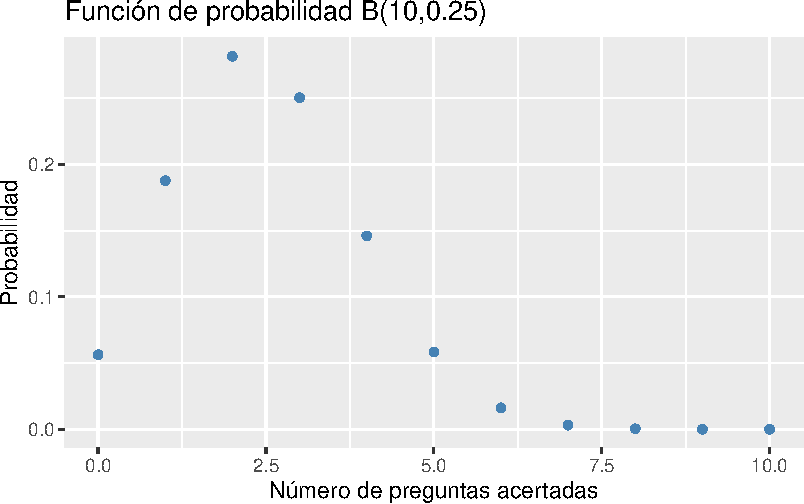
\includegraphics{06-distribuciones-probabilidad_files/figure-pdf/unnamed-chunk-5-1.pdf}

  La distribución es asimétrica hacia la derecha. A medida que aumenta
  el número de posibles respuestas, la probabilidad de acertar disminuye
  y la distribución binomial se hace más asimétrica hacia la derecha.

  \end{tcolorbox}
\item
  Dibujar la gráfica de la función de distribución del modelo de
  probabilidad anterior.

  \begin{tcolorbox}[enhanced jigsaw, toprule=.15mm, rightrule=.15mm, arc=.35mm, colback=white, colbacktitle=quarto-callout-tip-color!10!white, toptitle=1mm, left=2mm, colframe=quarto-callout-tip-color-frame, opacityback=0, breakable, opacitybacktitle=0.6, bottomtitle=1mm, titlerule=0mm, title=\textcolor{quarto-callout-tip-color}{\faLightbulb}\hspace{0.5em}{Solución}, bottomrule=.15mm, coltitle=black, leftrule=.75mm]

  Para calcular probabilidades acumuladas con el modelo binomial se
  utiliza la función
  \href{https://www.rdocumentation.org/packages/stats/versions/3.3/topics/Binomial}{\texttt{pbinom(x,\ n,\ p)}}
  del paquete \texttt{stats}, donde \texttt{n} es el número de
  repeticiones, \texttt{p} es la probabilidad de éxito, y \texttt{x} es
  el valor de la variable.

\begin{Shaded}
\begin{Highlighting}[]
\FunctionTok{library}\NormalTok{(ggplot2)}
\NormalTok{df}\SpecialCharTok{$}\NormalTok{F }\OtherTok{\textless{}{-}} \FunctionTok{pbinom}\NormalTok{(x, }\DecValTok{10}\NormalTok{, }\FloatTok{0.25}\NormalTok{)}
\FunctionTok{ggplot}\NormalTok{(df, }\FunctionTok{aes}\NormalTok{(}\AttributeTok{x =}\NormalTok{ x, }\AttributeTok{y =}\NormalTok{ F)) }\SpecialCharTok{+}
    \FunctionTok{geom\_point}\NormalTok{(}\AttributeTok{color =} \StringTok{"steelblue"}\NormalTok{) }\SpecialCharTok{+}
    \FunctionTok{labs}\NormalTok{(}\AttributeTok{title =} \StringTok{"Función de distribución B(10,0.25)"}\NormalTok{, }\AttributeTok{x =} \StringTok{"Número de preguntas acertadas"}\NormalTok{, }\AttributeTok{y =} \StringTok{"Probabilidad acumulada"}\NormalTok{)}
\end{Highlighting}
\end{Shaded}

  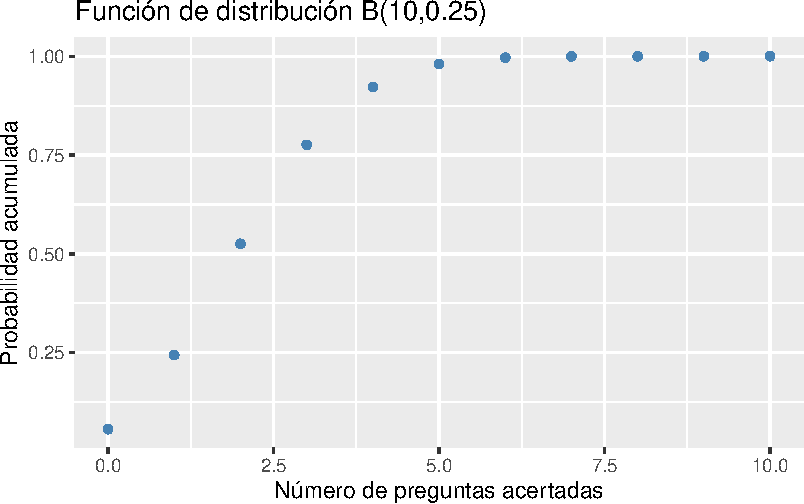
\includegraphics{06-distribuciones-probabilidad_files/figure-pdf/unnamed-chunk-6-1.pdf}

  La distribución es asimétrica hacia la derecha.

  \end{tcolorbox}
\item
  ¿Cuál es la probabilidad de sacar 3 puntos o menos en el test si se
  contestan todas las preguntas al azar?

  \begin{tcolorbox}[enhanced jigsaw, toprule=.15mm, rightrule=.15mm, arc=.35mm, colback=white, colbacktitle=quarto-callout-tip-color!10!white, toptitle=1mm, left=2mm, colframe=quarto-callout-tip-color-frame, opacityback=0, breakable, opacitybacktitle=0.6, bottomtitle=1mm, titlerule=0mm, title=\textcolor{quarto-callout-tip-color}{\faLightbulb}\hspace{0.5em}{Solución}, bottomrule=.15mm, coltitle=black, leftrule=.75mm]

\begin{Shaded}
\begin{Highlighting}[]
\FunctionTok{pbinom}\NormalTok{(}\DecValTok{3}\NormalTok{, }\DecValTok{10}\NormalTok{, }\FloatTok{0.25}\NormalTok{)}
\end{Highlighting}
\end{Shaded}

\begin{verbatim}
[1] 0.7758751
\end{verbatim}

  \end{tcolorbox}
\item
  ¿Cuál es la probabilidad de aprobar el test si se contestan todas las
  preguntas al azar?

  \begin{tcolorbox}[enhanced jigsaw, toprule=.15mm, rightrule=.15mm, arc=.35mm, colback=white, colbacktitle=quarto-callout-tip-color!10!white, toptitle=1mm, left=2mm, colframe=quarto-callout-tip-color-frame, opacityback=0, breakable, opacitybacktitle=0.6, bottomtitle=1mm, titlerule=0mm, title=\textcolor{quarto-callout-tip-color}{\faLightbulb}\hspace{0.5em}{Solución}, bottomrule=.15mm, coltitle=black, leftrule=.75mm]

  En este caso se trata de una probabilidad acumulada hacia la derecha,
  es decir, por encima del valor dado. Para ello hay que añadir el
  parámetro \texttt{lower.tail\ =\ FALSE} a la función \texttt{pbinom}.

  \begin{tcolorbox}[enhanced jigsaw, toprule=.15mm, rightrule=.15mm, arc=.35mm, colback=white, colbacktitle=quarto-callout-warning-color!10!white, toptitle=1mm, left=2mm, colframe=quarto-callout-warning-color-frame, opacityback=0, breakable, opacitybacktitle=0.6, bottomtitle=1mm, titlerule=0mm, title=\textcolor{quarto-callout-warning-color}{\faExclamationTriangle}\hspace{0.5em}{Advertencia}, bottomrule=.15mm, coltitle=black, leftrule=.75mm]

  Las funciones de distribución en \(R\) incluyen la probabilidad del
  valor dado cuando la cola de acumulación es hacia la izquierda, es
  decir, se calcula \(P(X\leq x)\), pero no lo incluyen cuando la cola
  de acumulación es hacia la derecha, es decir, se calcula \(P(X>x)\).

  \end{tcolorbox}

\begin{Shaded}
\begin{Highlighting}[]
\FunctionTok{pbinom}\NormalTok{(}\DecValTok{4}\NormalTok{, }\DecValTok{10}\NormalTok{, }\FloatTok{0.25}\NormalTok{, }\AttributeTok{lower.tail =} \ConstantTok{FALSE}\NormalTok{)}
\end{Highlighting}
\end{Shaded}

\begin{verbatim}
[1] 0.07812691
\end{verbatim}

\begin{Shaded}
\begin{Highlighting}[]
\CommentTok{\# o bien}
\DecValTok{1} \SpecialCharTok{{-}} \FunctionTok{pbinom}\NormalTok{(}\DecValTok{4}\NormalTok{, }\DecValTok{10}\NormalTok{, }\FloatTok{0.25}\NormalTok{)}
\end{Highlighting}
\end{Shaded}

\begin{verbatim}
[1] 0.07812691
\end{verbatim}

  \end{tcolorbox}
\item
  ¿Cuál es la probabilidad de tener un notable si se contestan todas las
  preguntas al azar?

  \begin{tcolorbox}[enhanced jigsaw, toprule=.15mm, rightrule=.15mm, arc=.35mm, colback=white, colbacktitle=quarto-callout-tip-color!10!white, toptitle=1mm, left=2mm, colframe=quarto-callout-tip-color-frame, opacityback=0, breakable, opacitybacktitle=0.6, bottomtitle=1mm, titlerule=0mm, title=\textcolor{quarto-callout-tip-color}{\faLightbulb}\hspace{0.5em}{Solución}, bottomrule=.15mm, coltitle=black, leftrule=.75mm]

  El notable se corresponde con una nota de 7 u 8, por lo que hay que
  calcular la probabilidad \(P(7\leq X\leq 8)\).

\begin{Shaded}
\begin{Highlighting}[]
\FunctionTok{pbinom}\NormalTok{(}\DecValTok{8}\NormalTok{, }\DecValTok{10}\NormalTok{, }\FloatTok{0.25}\NormalTok{) }\SpecialCharTok{{-}} \FunctionTok{pbinom}\NormalTok{(}\DecValTok{6}\NormalTok{, }\DecValTok{10}\NormalTok{, }\FloatTok{0.25}\NormalTok{)}
\end{Highlighting}
\end{Shaded}

\begin{verbatim}
[1] 0.003476143
\end{verbatim}

  \end{tcolorbox}
\end{enumerate}

\end{exercise}

\begin{exercise}[]\protect\hypertarget{exr-distribuciones-probabilidad-3}{}\label{exr-distribuciones-probabilidad-3}

El número medio de llamadas telefónicas que llegan a un servicio de
teleasistencia es de 4 por minuto en horario laborable.

\begin{enumerate}
\def\labelenumi{\alph{enumi}.}
\item
  ¿Qué tipo de modelo de distribución de probabilidad sigue la variable
  que mide el número de llamadas que llegan al servicio de
  teleasistencia en un minuto? Construir su función de probabilidad.

  \begin{tcolorbox}[enhanced jigsaw, toprule=.15mm, rightrule=.15mm, arc=.35mm, colback=white, colbacktitle=quarto-callout-tip-color!10!white, toptitle=1mm, left=2mm, colframe=quarto-callout-tip-color-frame, opacityback=0, breakable, opacitybacktitle=0.6, bottomtitle=1mm, titlerule=0mm, title=\textcolor{quarto-callout-tip-color}{\faLightbulb}\hspace{0.5em}{Solución}, bottomrule=.15mm, coltitle=black, leftrule=.75mm]

  Se trata de una
  \href{https://es.wikipedia.org/wiki/Distribuci\%C3\%B3n_de_Poisson}{distribución
  de Poisson} \(P(4)\). Para calcular probabilidades con el modelo
  Poisson se utiliza la función
  \href{https://www.rdocumentation.org/packages/stats/versions/3.6.2/topics/Poisson}{\texttt{dpois(x,\ lambda)}}
  del paquete \texttt{stats}, donde \texttt{lambda} es el número medio
  de sucesos en el intervalo considerado y \texttt{x} es el valor de la
  variable.

\begin{Shaded}
\begin{Highlighting}[]
\FunctionTok{library}\NormalTok{(kableExtra)}
\NormalTok{x }\OtherTok{\textless{}{-}} \DecValTok{0}\SpecialCharTok{:}\DecValTok{15}
\NormalTok{f }\OtherTok{\textless{}{-}} \FunctionTok{dpois}\NormalTok{(x, }\DecValTok{4}\NormalTok{)}
\NormalTok{df }\OtherTok{\textless{}{-}} \FunctionTok{data.frame}\NormalTok{(x, f)}
\NormalTok{df }\SpecialCharTok{|\textgreater{}} 
    \FunctionTok{kable}\NormalTok{() }\SpecialCharTok{|\textgreater{}} 
    \FunctionTok{kable\_styling}\NormalTok{(}\AttributeTok{full\_width =}\NormalTok{ F)}
\end{Highlighting}
\end{Shaded}

  \begin{table}
  \centering
  \begin{tabular}{r|r}
  \hline
  x & f\\
  \hline
  0 & 0.0183156\\
  \hline
  1 & 0.0732626\\
  \hline
  2 & 0.1465251\\
  \hline
  3 & 0.1953668\\
  \hline
  4 & 0.1953668\\
  \hline
  5 & 0.1562935\\
  \hline
  6 & 0.1041956\\
  \hline
  7 & 0.0595404\\
  \hline
  8 & 0.0297702\\
  \hline
  9 & 0.0132312\\
  \hline
  10 & 0.0052925\\
  \hline
  11 & 0.0019245\\
  \hline
  12 & 0.0006415\\
  \hline
  13 & 0.0001974\\
  \hline
  14 & 0.0000564\\
  \hline
  15 & 0.0000150\\
  \hline
  \end{tabular}
  \end{table}

  \end{tcolorbox}
\item
  Dibujar la gráfica de la función de probabilidad del modelo de
  probabilidad anterior. ¿Cómo es la asimetría de la distribución de
  probabilidad?

  \begin{tcolorbox}[enhanced jigsaw, toprule=.15mm, rightrule=.15mm, arc=.35mm, colback=white, colbacktitle=quarto-callout-tip-color!10!white, toptitle=1mm, left=2mm, colframe=quarto-callout-tip-color-frame, opacityback=0, breakable, opacitybacktitle=0.6, bottomtitle=1mm, titlerule=0mm, title=\textcolor{quarto-callout-tip-color}{\faLightbulb}\hspace{0.5em}{Solución}, bottomrule=.15mm, coltitle=black, leftrule=.75mm]

\begin{Shaded}
\begin{Highlighting}[]
\FunctionTok{library}\NormalTok{(ggplot2)}
\FunctionTok{ggplot}\NormalTok{(df, }\FunctionTok{aes}\NormalTok{(}\AttributeTok{x =}\NormalTok{ x, }\AttributeTok{y =}\NormalTok{ f)) }\SpecialCharTok{+}
    \FunctionTok{geom\_point}\NormalTok{(}\AttributeTok{color =} \StringTok{"steelblue"}\NormalTok{) }\SpecialCharTok{+}
    \FunctionTok{labs}\NormalTok{(}\AttributeTok{title =} \StringTok{"Función de probabilidad P(4)"}\NormalTok{, }\AttributeTok{x =} \StringTok{"Número de llamadas en 1 minuto"}\NormalTok{, }\AttributeTok{y =} \StringTok{"Probabilidad"}\NormalTok{)}
\end{Highlighting}
\end{Shaded}

  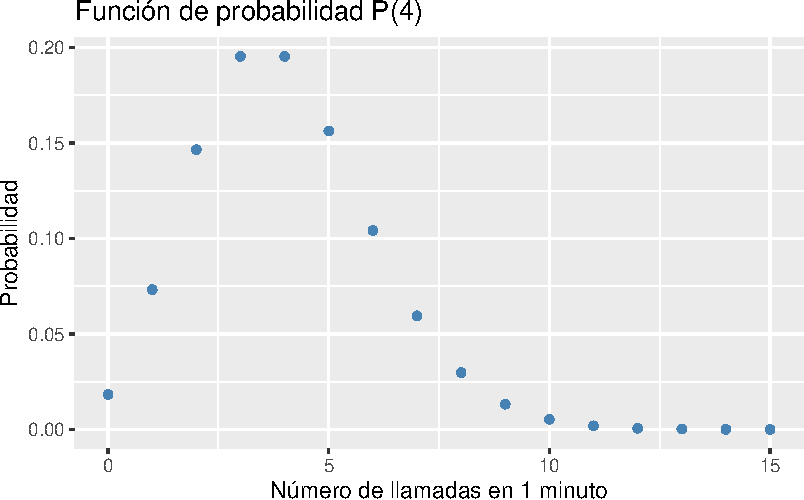
\includegraphics{06-distribuciones-probabilidad_files/figure-pdf/unnamed-chunk-11-1.pdf}

  La distribución es asimétrica hacia la derecha.

  \end{tcolorbox}
\item
  ¿Cuál es la probabilidad de que lleguen menos de 2 llamadas en un
  minuto?

  \begin{tcolorbox}[enhanced jigsaw, toprule=.15mm, rightrule=.15mm, arc=.35mm, colback=white, colbacktitle=quarto-callout-tip-color!10!white, toptitle=1mm, left=2mm, colframe=quarto-callout-tip-color-frame, opacityback=0, breakable, opacitybacktitle=0.6, bottomtitle=1mm, titlerule=0mm, title=\textcolor{quarto-callout-tip-color}{\faLightbulb}\hspace{0.5em}{Solución}, bottomrule=.15mm, coltitle=black, leftrule=.75mm]

\begin{Shaded}
\begin{Highlighting}[]
\FunctionTok{ppois}\NormalTok{(}\DecValTok{1}\NormalTok{, }\DecValTok{4}\NormalTok{)}
\end{Highlighting}
\end{Shaded}

\begin{verbatim}
[1] 0.09157819
\end{verbatim}

  \end{tcolorbox}
\item
  Si la empresa que da el servicio tiene operadores para atener como
  máximo 30 llamadas cada 5 minutos, ¿cuál es la probabilidad de que en
  un intervalo de 5 minutos no se puedan atender todas las llamadas?

  \begin{tcolorbox}[enhanced jigsaw, toprule=.15mm, rightrule=.15mm, arc=.35mm, colback=white, colbacktitle=quarto-callout-tip-color!10!white, toptitle=1mm, left=2mm, colframe=quarto-callout-tip-color-frame, opacityback=0, breakable, opacitybacktitle=0.6, bottomtitle=1mm, titlerule=0mm, title=\textcolor{quarto-callout-tip-color}{\faLightbulb}\hspace{0.5em}{Solución}, bottomrule=.15mm, coltitle=black, leftrule=.75mm]

  Como el intervalo de tiempo ahora es de 5 minutos, el número medio de
  llamadas en este intervalo de tiempo es 4\cdot 5 = 20, y por tanto,
  hay que trabajar con un modelo de Poisson \(P(20)\).

  Por otro lado, como ahora queremos calcular una probabilidad acumulada
  hacia la derechea, es decir, por encima del valor, hay que añadir el
  parámetro \texttt{lower.tail\ =\ FALSE} a la función \texttt{ppois}.

\begin{Shaded}
\begin{Highlighting}[]
\FunctionTok{ppois}\NormalTok{(}\DecValTok{30}\NormalTok{, }\DecValTok{20}\NormalTok{, }\AttributeTok{lower.tail =} \ConstantTok{FALSE}\NormalTok{)}
\end{Highlighting}
\end{Shaded}

\begin{verbatim}
[1] 0.01347468
\end{verbatim}

  \end{tcolorbox}
\end{enumerate}

\end{exercise}

\begin{exercise}[]\protect\hypertarget{exr-distribuciones-probabilidad-4}{}\label{exr-distribuciones-probabilidad-4}

La \href{https://en.wikipedia.org/wiki/Poisson_limit_theorem}{ley de los
casos raros} establece que la función de probabilidad de un modelo de
Poison \(P(\lambda)\) se obtiene en el límite cuando \(n\) tiende a
\(\infty\) y \(p\) tiende a \(0\) de la función de probabilidad de un
modelo Binomial \(B(n,p)\), donde \(\lambda = np\).

\begin{enumerate}
\def\labelenumi{\alph{enumi}.}
\item
  Aproximar un modelo binomial \(B(10, 0.2)\) mediante el
  correspondiente modelo Poisson aplicando la ley de los casos raros y
  comparar las gráficas de las distribuciones de probabilidad de ambos
  modelos. ¿Es una buena aproximación?

  \begin{tcolorbox}[enhanced jigsaw, toprule=.15mm, rightrule=.15mm, arc=.35mm, colback=white, colbacktitle=quarto-callout-tip-color!10!white, toptitle=1mm, left=2mm, colframe=quarto-callout-tip-color-frame, opacityback=0, breakable, opacitybacktitle=0.6, bottomtitle=1mm, titlerule=0mm, title=\textcolor{quarto-callout-tip-color}{\faLightbulb}\hspace{0.5em}{Solución}, bottomrule=.15mm, coltitle=black, leftrule=.75mm]

  Según la ley de los casos raros \(B(10, 0.3) \approx P(3)\).

\begin{Shaded}
\begin{Highlighting}[]
\FunctionTok{library}\NormalTok{(kableExtra)}
\FunctionTok{library}\NormalTok{(tidyverse)}
\FunctionTok{library}\NormalTok{(ggplot2)}
\NormalTok{x }\OtherTok{\textless{}{-}} \DecValTok{0}\SpecialCharTok{:}\DecValTok{10}
\NormalTok{fbinom }\OtherTok{\textless{}{-}} \FunctionTok{dbinom}\NormalTok{(x, }\DecValTok{10}\NormalTok{, }\FloatTok{0.3}\NormalTok{)}
\NormalTok{fpois }\OtherTok{\textless{}{-}} \FunctionTok{dpois}\NormalTok{(x, }\DecValTok{3}\NormalTok{)}
\NormalTok{df }\OtherTok{\textless{}{-}} \FunctionTok{data.frame}\NormalTok{(x, fbinom, fpois)}
\NormalTok{df  }\SpecialCharTok{|\textgreater{}} 
    \FunctionTok{pivot\_longer}\NormalTok{(}\SpecialCharTok{{-}}\NormalTok{x, }\AttributeTok{names\_to =} \StringTok{"Distribución"}\NormalTok{, }\AttributeTok{values\_to =} \StringTok{"Probabilidad"}\NormalTok{)  }\SpecialCharTok{|\textgreater{}} 
    \FunctionTok{ggplot}\NormalTok{(}\FunctionTok{aes}\NormalTok{(}\AttributeTok{x =}\NormalTok{ x, }\AttributeTok{y =}\NormalTok{ Probabilidad, }\AttributeTok{color =}\NormalTok{ Distribución)) }\SpecialCharTok{+} 
    \FunctionTok{geom\_point}\NormalTok{() }\SpecialCharTok{+}
    \FunctionTok{labs}\NormalTok{(}\AttributeTok{title =} \StringTok{"Función de probabilidad de los modelos B(10, 0.3) y P(3)"}\NormalTok{)}
\end{Highlighting}
\end{Shaded}

  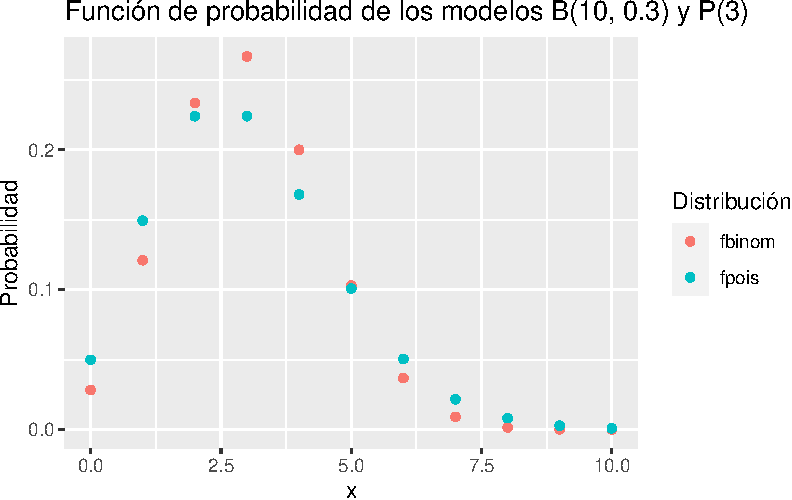
\includegraphics{06-distribuciones-probabilidad_files/figure-pdf/unnamed-chunk-14-1.pdf}

  Vamos a calcular el error en la aproximación.

\begin{Shaded}
\begin{Highlighting}[]
\NormalTok{df  }\SpecialCharTok{|\textgreater{}} 
    \FunctionTok{mutate}\NormalTok{(}\AttributeTok{error =} \FunctionTok{abs}\NormalTok{(fbinom }\SpecialCharTok{{-}}\NormalTok{ fpois))  }\SpecialCharTok{|\textgreater{}} 
    \FunctionTok{summarize}\NormalTok{(}\AttributeTok{error =} \FunctionTok{sum}\NormalTok{(error))}
\end{Highlighting}
\end{Shaded}

\begin{verbatim}
      error
1 0.1725254
\end{verbatim}

  Así pues, la aproximación no es buena pues el error es mayor del 17\%.

  \end{tcolorbox}
\item
  Aproximar \(B(30, 0.1)\) mediante el correspondiente modelo Poisson
  aplicando la ley de los casos raros y comparar las gráficas de las
  distribuciones de probabilidad de ambos modelos. ¿Es una buena
  aproximación?

  \begin{tcolorbox}[enhanced jigsaw, toprule=.15mm, rightrule=.15mm, arc=.35mm, colback=white, colbacktitle=quarto-callout-tip-color!10!white, toptitle=1mm, left=2mm, colframe=quarto-callout-tip-color-frame, opacityback=0, breakable, opacitybacktitle=0.6, bottomtitle=1mm, titlerule=0mm, title=\textcolor{quarto-callout-tip-color}{\faLightbulb}\hspace{0.5em}{Solución}, bottomrule=.15mm, coltitle=black, leftrule=.75mm]

  Según la ley de los casos raros \(B(30, 0.1) \approx P(3)\).

\begin{Shaded}
\begin{Highlighting}[]
\NormalTok{x }\OtherTok{\textless{}{-}} \DecValTok{0}\SpecialCharTok{:}\DecValTok{30}
\NormalTok{fbinom }\OtherTok{\textless{}{-}} \FunctionTok{dbinom}\NormalTok{(x, }\DecValTok{30}\NormalTok{, }\FloatTok{0.1}\NormalTok{)}
\NormalTok{fpois }\OtherTok{\textless{}{-}} \FunctionTok{dpois}\NormalTok{(x, }\DecValTok{3}\NormalTok{)}
\NormalTok{df }\OtherTok{\textless{}{-}} \FunctionTok{data.frame}\NormalTok{(x, fbinom, fpois)}
\NormalTok{df  }\SpecialCharTok{|\textgreater{}} 
    \FunctionTok{pivot\_longer}\NormalTok{(}\SpecialCharTok{{-}}\NormalTok{x, }\AttributeTok{names\_to =} \StringTok{"Distribución"}\NormalTok{, }\AttributeTok{values\_to =} \StringTok{"Probabilidad"}\NormalTok{)  }\SpecialCharTok{|\textgreater{}} 
    \FunctionTok{ggplot}\NormalTok{(}\FunctionTok{aes}\NormalTok{(}\AttributeTok{x =}\NormalTok{ x, }\AttributeTok{y =}\NormalTok{ Probabilidad, }\AttributeTok{color =}\NormalTok{ Distribución)) }\SpecialCharTok{+} 
    \FunctionTok{geom\_point}\NormalTok{() }\SpecialCharTok{+}
    \FunctionTok{labs}\NormalTok{(}\AttributeTok{title =} \StringTok{"Función de probabilidad de los modelos B(30, 0.1) y P(3)"}\NormalTok{)}
\end{Highlighting}
\end{Shaded}

  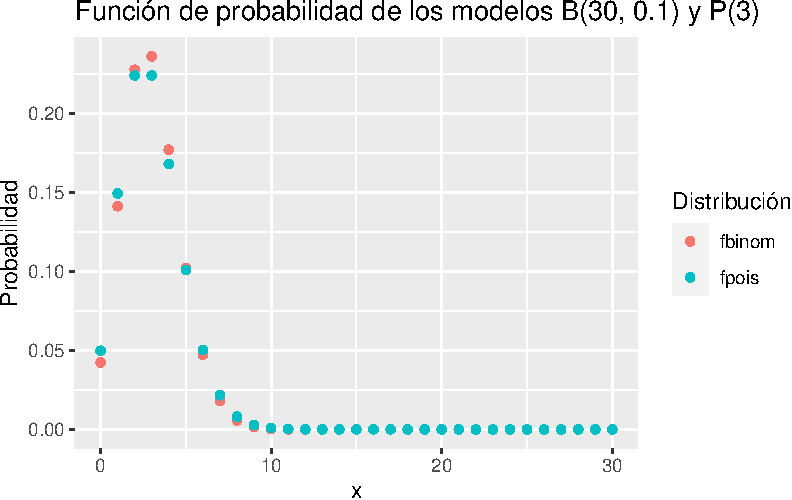
\includegraphics{06-distribuciones-probabilidad_files/figure-pdf/unnamed-chunk-16-1.pdf}

  Vamos a calcular el error en la aproximación.

\begin{Shaded}
\begin{Highlighting}[]
\NormalTok{df  }\SpecialCharTok{|\textgreater{}} 
    \FunctionTok{mutate}\NormalTok{(}\AttributeTok{error =} \FunctionTok{abs}\NormalTok{(fbinom }\SpecialCharTok{{-}}\NormalTok{ fpois))  }\SpecialCharTok{|\textgreater{}} 
    \FunctionTok{summarize}\NormalTok{(}\AttributeTok{error =} \FunctionTok{sum}\NormalTok{(error))}
\end{Highlighting}
\end{Shaded}

\begin{verbatim}
       error
1 0.05236218
\end{verbatim}

  Ahora la aproximación es mucho mejor, ya que el error es menor del
  5\%.

  \end{tcolorbox}
\item
  Definir una función para repetir los procedimientos de los apartados
  anteriores para cualquier modelo binomial, y utilizarla para una
  binomial \(B(100, 0.03)\).

  \begin{tcolorbox}[enhanced jigsaw, toprule=.15mm, rightrule=.15mm, arc=.35mm, colback=white, colbacktitle=quarto-callout-tip-color!10!white, toptitle=1mm, left=2mm, colframe=quarto-callout-tip-color-frame, opacityback=0, breakable, opacitybacktitle=0.6, bottomtitle=1mm, titlerule=0mm, title=\textcolor{quarto-callout-tip-color}{\faLightbulb}\hspace{0.5em}{Solución}, bottomrule=.15mm, coltitle=black, leftrule=.75mm]

\begin{Shaded}
\begin{Highlighting}[]
\NormalTok{casos\_raros }\OtherTok{\textless{}{-}} \ControlFlowTok{function}\NormalTok{ (n, p)\{}
    \CommentTok{\# Definimos el rango del modelo binomial.}
\NormalTok{    x }\OtherTok{\textless{}{-}} \DecValTok{0}\SpecialCharTok{:}\NormalTok{n}
    \CommentTok{\# Función de probabilidad del modelo binomial.}
\NormalTok{    fbinom }\OtherTok{\textless{}{-}} \FunctionTok{dbinom}\NormalTok{(x, n, p)}
    \CommentTok{\# Función de distribución del modelo Poisson equivalente.}
\NormalTok{    fpois }\OtherTok{\textless{}{-}} \FunctionTok{dpois}\NormalTok{(x, n}\SpecialCharTok{*}\NormalTok{p)}
    \CommentTok{\# Creamos un data frame con las dos funciones de probabilidad.}
\NormalTok{    df }\OtherTok{\textless{}{-}} \FunctionTok{data.frame}\NormalTok{(x, fbinom, fpois)}
    \CommentTok{\# Dibujamos las gráficas de las funciones de probabilidad.}
\NormalTok{    grafico }\OtherTok{\textless{}{-}}\NormalTok{ df  }\SpecialCharTok{|\textgreater{}} 
        \FunctionTok{pivot\_longer}\NormalTok{(}\SpecialCharTok{{-}}\NormalTok{x, }\AttributeTok{names\_to =} \StringTok{"Distribución"}\NormalTok{, }\AttributeTok{values\_to =} \StringTok{"Probabilidad"}\NormalTok{)  }\SpecialCharTok{|\textgreater{}} 
        \FunctionTok{ggplot}\NormalTok{(}\FunctionTok{aes}\NormalTok{(}\AttributeTok{x =}\NormalTok{ x, }\AttributeTok{y =}\NormalTok{ Probabilidad, }\AttributeTok{color =}\NormalTok{ Distribución)) }\SpecialCharTok{+} 
        \FunctionTok{geom\_point}\NormalTok{() }\SpecialCharTok{+}
        \FunctionTok{labs}\NormalTok{(}\AttributeTok{title =} \FunctionTok{paste0}\NormalTok{(}\StringTok{"Función de probabilidad de los modelos B("}\NormalTok{, n, }\StringTok{","}\NormalTok{, p, }\StringTok{") y P("}\NormalTok{, n}\SpecialCharTok{*}\NormalTok{p, }\StringTok{")"}\NormalTok{))}
    \CommentTok{\# Calculamos el error de la aproximación.}
\NormalTok{    error }\OtherTok{\textless{}{-}}\NormalTok{ df  }\SpecialCharTok{|\textgreater{}} 
        \FunctionTok{mutate}\NormalTok{(}\AttributeTok{error =} \FunctionTok{abs}\NormalTok{(fbinom }\SpecialCharTok{{-}}\NormalTok{ fpois))  }\SpecialCharTok{|\textgreater{}} 
        \FunctionTok{summarize}\NormalTok{(}\AttributeTok{error =} \FunctionTok{sum}\NormalTok{(error))}
    \FunctionTok{return}\NormalTok{(}\FunctionTok{list}\NormalTok{(grafico, error))}
\NormalTok{\}}

\FunctionTok{casos\_raros}\NormalTok{(}\DecValTok{100}\NormalTok{, }\FloatTok{0.03}\NormalTok{) }
\end{Highlighting}
\end{Shaded}

\begin{verbatim}
[[1]]
\end{verbatim}

  \includegraphics{06-distribuciones-probabilidad_files/figure-pdf/unnamed-chunk-18-1.pdf}

\begin{verbatim}

[[2]]
       error
1 0.01521393
\end{verbatim}

  \end{tcolorbox}
\item
  Dibujar una gráfica con los errores en las aproximaciones de un modelo
  binomial \(B(n,p)\) mediante un modelo Poisson \(P(3)\) para valores
  de \$n desde \(n=4\) hasta \(n=100\). ¿A partir de que \(n\) la ley de
  los casos raros da un error menor del 5\%?

  \begin{tcolorbox}[enhanced jigsaw, toprule=.15mm, rightrule=.15mm, arc=.35mm, colback=white, colbacktitle=quarto-callout-tip-color!10!white, toptitle=1mm, left=2mm, colframe=quarto-callout-tip-color-frame, opacityback=0, breakable, opacitybacktitle=0.6, bottomtitle=1mm, titlerule=0mm, title=\textcolor{quarto-callout-tip-color}{\faLightbulb}\hspace{0.5em}{Solución}, bottomrule=.15mm, coltitle=black, leftrule=.75mm]

\begin{Shaded}
\begin{Highlighting}[]
\FunctionTok{library}\NormalTok{(purrr)}
\NormalTok{error\_casos\_raros }\OtherTok{\textless{}{-}} \ControlFlowTok{function}\NormalTok{ (n)\{}
    \CommentTok{\# Definimos el rango del modelo binomial.}
\NormalTok{    x }\OtherTok{\textless{}{-}} \DecValTok{0}\SpecialCharTok{:}\NormalTok{n}
    \CommentTok{\# Función de probabilidad del modelo binomial.}
\NormalTok{    fbinom }\OtherTok{\textless{}{-}} \FunctionTok{dbinom}\NormalTok{(x, n, }\DecValTok{3}\SpecialCharTok{/}\NormalTok{n)}
    \CommentTok{\# Función de distribución del modelo Poisson equivalente.}
\NormalTok{    fpois }\OtherTok{\textless{}{-}} \FunctionTok{dpois}\NormalTok{(x, }\DecValTok{3}\NormalTok{)}
    \CommentTok{\# Calculamos los errores para cada n.}
\NormalTok{    error }\OtherTok{=} \FunctionTok{abs}\NormalTok{(fbinom }\SpecialCharTok{{-}}\NormalTok{ fpois)}
    \CommentTok{\# Devolvemos la suma de los errores}
    \FunctionTok{return}\NormalTok{(}\FunctionTok{sum}\NormalTok{(error))}
\NormalTok{\}}

\FunctionTok{data.frame}\NormalTok{(}\AttributeTok{n =} \DecValTok{4}\SpecialCharTok{:}\DecValTok{100}\NormalTok{)  }\SpecialCharTok{|\textgreater{}} 
    \FunctionTok{mutate}\NormalTok{(}\AttributeTok{error =} \FunctionTok{map\_dbl}\NormalTok{(n, error\_casos\_raros))  }\SpecialCharTok{|\textgreater{}} 
    \FunctionTok{ggplot}\NormalTok{(}\FunctionTok{aes}\NormalTok{(}\AttributeTok{x =}\NormalTok{ n, }\AttributeTok{y =}\NormalTok{ error)) }\SpecialCharTok{+}
    \FunctionTok{geom\_point}\NormalTok{(}\AttributeTok{color =} \StringTok{"steelblue"}\NormalTok{) }\SpecialCharTok{+}
    \FunctionTok{geom\_hline}\NormalTok{(}\AttributeTok{yintercept =} \FloatTok{0.05}\NormalTok{, }\AttributeTok{color =} \StringTok{"red"}\NormalTok{) }\SpecialCharTok{+}
    \FunctionTok{labs}\NormalTok{(}\AttributeTok{title =} \StringTok{"Error en la aproximación de un modelo B(n,p) con otro P(np)"}\NormalTok{)}
\end{Highlighting}
\end{Shaded}

  \includegraphics{06-distribuciones-probabilidad_files/figure-pdf/unnamed-chunk-19-1.pdf}

  \end{tcolorbox}
\end{enumerate}

\end{exercise}

\begin{exercise}[]\protect\hypertarget{exr-distribuciones-probabilidad-5}{}\label{exr-distribuciones-probabilidad-5}

La vida media de un tipo de batería es de 50 días.

\begin{enumerate}
\def\labelenumi{\alph{enumi}.}
\item
  ¿Qué tipo de modelo de distribución de probabilidad sigue la variable
  que mide la duración de este tipo de baterías? Construir su función de
  densidad.

  \begin{tcolorbox}[enhanced jigsaw, toprule=.15mm, rightrule=.15mm, arc=.35mm, colback=white, colbacktitle=quarto-callout-tip-color!10!white, toptitle=1mm, left=2mm, colframe=quarto-callout-tip-color-frame, opacityback=0, breakable, opacitybacktitle=0.6, bottomtitle=1mm, titlerule=0mm, title=\textcolor{quarto-callout-tip-color}{\faLightbulb}\hspace{0.5em}{Solución}, bottomrule=.15mm, coltitle=black, leftrule=.75mm]

  Se trata de una
  \href{https://es.wikipedia.org/wiki/Distribuci\%C3\%B3n_exponencial}{distribución
  exponencial} \(Exp(1/50)\). Para calcular probabilidades con el modelo
  exponencial se utiliza la función
  \href{https://www.rdocumentation.org/packages/stats/versions/3.3/topics/Exponential}{\texttt{dexp(x,\ lambda)}}
  del paquete \texttt{stats}, donde \texttt{lambda} es el inverso de la
  media y \texttt{x} es el valor de la variable.

\begin{Shaded}
\begin{Highlighting}[]
\NormalTok{x }\OtherTok{\textless{}{-}} \FunctionTok{seq}\NormalTok{(}\DecValTok{0}\NormalTok{,}\DecValTok{300}\NormalTok{,}\FloatTok{0.1}\NormalTok{)}
\NormalTok{f }\OtherTok{\textless{}{-}} \FunctionTok{dexp}\NormalTok{(x, }\DecValTok{1}\SpecialCharTok{/}\DecValTok{50}\NormalTok{)}
\NormalTok{df }\OtherTok{\textless{}{-}} \FunctionTok{data.frame}\NormalTok{(x, f)}
\FunctionTok{ggplot}\NormalTok{(df, }\FunctionTok{aes}\NormalTok{(}\AttributeTok{x =}\NormalTok{ x, }\AttributeTok{y =}\NormalTok{ f)) }\SpecialCharTok{+}
    \FunctionTok{geom\_line}\NormalTok{(}\AttributeTok{color =} \StringTok{"steelblue"}\NormalTok{) }\SpecialCharTok{+}
    \FunctionTok{labs}\NormalTok{(}\AttributeTok{title =} \StringTok{"Función de densidad Exp(1/50)"}\NormalTok{, }\AttributeTok{x =} \StringTok{"Días de duración"}\NormalTok{, }\AttributeTok{y =} \StringTok{"Densidad de probabilidad"}\NormalTok{)}
\end{Highlighting}
\end{Shaded}

  \includegraphics{06-distribuciones-probabilidad_files/figure-pdf/unnamed-chunk-20-1.pdf}

  \end{tcolorbox}
\item
  Calcula la probabilidad de que la batería dure menos de 50 días.

  \begin{tcolorbox}[enhanced jigsaw, toprule=.15mm, rightrule=.15mm, arc=.35mm, colback=white, colbacktitle=quarto-callout-tip-color!10!white, toptitle=1mm, left=2mm, colframe=quarto-callout-tip-color-frame, opacityback=0, breakable, opacitybacktitle=0.6, bottomtitle=1mm, titlerule=0mm, title=\textcolor{quarto-callout-tip-color}{\faLightbulb}\hspace{0.5em}{Solución}, bottomrule=.15mm, coltitle=black, leftrule=.75mm]

  Para calcular probabilidades con el modelo exponencial se utiliza la
  función
  \href{https://www.rdocumentation.org/packages/stats/versions/3.3/topics/Exponential}{\texttt{pexp(x,\ lambda)}}
  del paquete \texttt{stats}, donde \texttt{lambda} es el inverso de la
  media y \texttt{x} es el valor de la variable.

\begin{Shaded}
\begin{Highlighting}[]
\FunctionTok{pexp}\NormalTok{(}\DecValTok{50}\NormalTok{, }\DecValTok{1}\SpecialCharTok{/}\DecValTok{50}\NormalTok{)}
\end{Highlighting}
\end{Shaded}

\begin{verbatim}
[1] 0.6321206
\end{verbatim}

  \end{tcolorbox}
\item
  Calcula la probabilidad de que la batería dure más de 100 días.

  \begin{tcolorbox}[enhanced jigsaw, toprule=.15mm, rightrule=.15mm, arc=.35mm, colback=white, colbacktitle=quarto-callout-tip-color!10!white, toptitle=1mm, left=2mm, colframe=quarto-callout-tip-color-frame, opacityback=0, breakable, opacitybacktitle=0.6, bottomtitle=1mm, titlerule=0mm, title=\textcolor{quarto-callout-tip-color}{\faLightbulb}\hspace{0.5em}{Solución}, bottomrule=.15mm, coltitle=black, leftrule=.75mm]

  En este caso hay que calcular una probabilidad acumulada hacia la
  derecha, es decir, por encima del valor dado. Para ello hay añadir el
  parámetro \texttt{lower.tail\ =\ FALSE} a la función \texttt{pexp}.

\begin{Shaded}
\begin{Highlighting}[]
\FunctionTok{pexp}\NormalTok{(}\DecValTok{100}\NormalTok{, }\DecValTok{1}\SpecialCharTok{/}\DecValTok{50}\NormalTok{, }\AttributeTok{lower.tail =} \ConstantTok{FALSE}\NormalTok{)}
\end{Highlighting}
\end{Shaded}

\begin{verbatim}
[1] 0.1353353
\end{verbatim}

  \end{tcolorbox}
\item
  Calcula la probabilidad de que la batería dure entre 50 y 100 días.

  \begin{tcolorbox}[enhanced jigsaw, toprule=.15mm, rightrule=.15mm, arc=.35mm, colback=white, colbacktitle=quarto-callout-tip-color!10!white, toptitle=1mm, left=2mm, colframe=quarto-callout-tip-color-frame, opacityback=0, breakable, opacitybacktitle=0.6, bottomtitle=1mm, titlerule=0mm, title=\textcolor{quarto-callout-tip-color}{\faLightbulb}\hspace{0.5em}{Solución}, bottomrule=.15mm, coltitle=black, leftrule=.75mm]

\begin{Shaded}
\begin{Highlighting}[]
\FunctionTok{pexp}\NormalTok{(}\DecValTok{100}\NormalTok{, }\DecValTok{1}\SpecialCharTok{/}\DecValTok{50}\NormalTok{) }\SpecialCharTok{{-}} \FunctionTok{pexp}\NormalTok{(}\DecValTok{50}\NormalTok{, }\DecValTok{1}\SpecialCharTok{/}\DecValTok{50}\NormalTok{)}
\end{Highlighting}
\end{Shaded}

\begin{verbatim}
[1] 0.2325442
\end{verbatim}

  \end{tcolorbox}
\item
  Calcular los cuartiles de la distribución del tiempo de duración de
  las baterías.

  \begin{tcolorbox}[enhanced jigsaw, toprule=.15mm, rightrule=.15mm, arc=.35mm, colback=white, colbacktitle=quarto-callout-tip-color!10!white, toptitle=1mm, left=2mm, colframe=quarto-callout-tip-color-frame, opacityback=0, breakable, opacitybacktitle=0.6, bottomtitle=1mm, titlerule=0mm, title=\textcolor{quarto-callout-tip-color}{\faLightbulb}\hspace{0.5em}{Solución}, bottomrule=.15mm, coltitle=black, leftrule=.75mm]

  Para calcular percentiles con el modelo exponencial se utiliza la
  función
  \href{https://www.rdocumentation.org/packages/stats/versions/3.3/topics/Exponential}{\texttt{qexp(x,\ lambda)}}
  del paquete \texttt{stats}, donde \texttt{lambda} es el inverso de la
  media y \texttt{x} es la probabilidad acumulada del percentil.

\begin{Shaded}
\begin{Highlighting}[]
\NormalTok{cuartiles }\OtherTok{\textless{}{-}} \FunctionTok{qexp}\NormalTok{(}\FunctionTok{c}\NormalTok{(}\FloatTok{0.25}\NormalTok{, }\FloatTok{0.5}\NormalTok{, }\FloatTok{0.75}\NormalTok{), }\DecValTok{1}\SpecialCharTok{/}\DecValTok{50}\NormalTok{)}
\FunctionTok{names}\NormalTok{(cuartiles) }\OtherTok{\textless{}{-}} \FunctionTok{c}\NormalTok{(}\StringTok{"C1"}\NormalTok{, }\StringTok{"C2"}\NormalTok{, }\StringTok{"C3"}\NormalTok{)}
\NormalTok{cuartiles}
\end{Highlighting}
\end{Shaded}

\begin{verbatim}
      C1       C2       C3 
14.38410 34.65736 69.31472 
\end{verbatim}

  \end{tcolorbox}
\end{enumerate}

\end{exercise}

\begin{exercise}[]\protect\hypertarget{exr-distribuciones-probabilidad-6}{}\label{exr-distribuciones-probabilidad-6}

Se sabe que el nivel de colesterol en hombres de una determinada
población sigue una distribución Normal \(N(220, 20)\) en mg/dl.

\begin{enumerate}
\def\labelenumi{\alph{enumi}.}
\item
  Dibujar la función de densidad de este modelo.

  \begin{tcolorbox}[enhanced jigsaw, toprule=.15mm, rightrule=.15mm, arc=.35mm, colback=white, colbacktitle=quarto-callout-tip-color!10!white, toptitle=1mm, left=2mm, colframe=quarto-callout-tip-color-frame, opacityback=0, breakable, opacitybacktitle=0.6, bottomtitle=1mm, titlerule=0mm, title=\textcolor{quarto-callout-tip-color}{\faLightbulb}\hspace{0.5em}{Solución}, bottomrule=.15mm, coltitle=black, leftrule=.75mm]

  Para calcular densidades de probabilidad de una
  \href{https://es.wikipedia.org/wiki/Distribuci\%C3\%B3n_normal}{distribución
  normal} se utiliza la función
  \href{https://www.rdocumentation.org/packages/stats/versions/3.3/topics/Normal}{\texttt{dnorm(x,\ mean,\ sd)}}
  del paquete \texttt{stats}, donde \texttt{mean} es la media,
  \texttt{sd} es la desviación típica y \texttt{x} es el valor de la
  variable.

\begin{Shaded}
\begin{Highlighting}[]
\NormalTok{x }\OtherTok{\textless{}{-}} \FunctionTok{seq}\NormalTok{(}\DecValTok{160}\NormalTok{,}\DecValTok{280}\NormalTok{,}\FloatTok{0.1}\NormalTok{)}
\NormalTok{f }\OtherTok{\textless{}{-}} \FunctionTok{dnorm}\NormalTok{(x, }\DecValTok{220}\NormalTok{, }\DecValTok{20}\NormalTok{)}
\NormalTok{df }\OtherTok{\textless{}{-}} \FunctionTok{data.frame}\NormalTok{(x, f)}
\FunctionTok{ggplot}\NormalTok{(df, }\FunctionTok{aes}\NormalTok{(}\AttributeTok{x =}\NormalTok{ x, }\AttributeTok{y =}\NormalTok{ f)) }\SpecialCharTok{+}
    \FunctionTok{geom\_line}\NormalTok{(}\AttributeTok{color =} \StringTok{"steelblue"}\NormalTok{) }\SpecialCharTok{+}
    \FunctionTok{labs}\NormalTok{(}\AttributeTok{title =} \StringTok{"Función de densidad N(220,20)"}\NormalTok{, }\AttributeTok{x =} \StringTok{"Nivel de colesterol"}\NormalTok{, }\AttributeTok{y =} \StringTok{"Densidad de probabilidad"}\NormalTok{)}
\end{Highlighting}
\end{Shaded}

  \includegraphics{06-distribuciones-probabilidad_files/figure-pdf/unnamed-chunk-25-1.pdf}

  \end{tcolorbox}
\item
  Dibujar la gráfica de la función de distribución del modelo de
  probabilidad anterior.

  \begin{tcolorbox}[enhanced jigsaw, toprule=.15mm, rightrule=.15mm, arc=.35mm, colback=white, colbacktitle=quarto-callout-tip-color!10!white, toptitle=1mm, left=2mm, colframe=quarto-callout-tip-color-frame, opacityback=0, breakable, opacitybacktitle=0.6, bottomtitle=1mm, titlerule=0mm, title=\textcolor{quarto-callout-tip-color}{\faLightbulb}\hspace{0.5em}{Solución}, bottomrule=.15mm, coltitle=black, leftrule=.75mm]

  Para calcular probabilidades acumuladas con el modelo normal se
  utiliza la función
  \href{https://www.rdocumentation.org/packages/stats/versions/3.3/topics/Normal}{\texttt{pnorm(x,\ mean,\ sd)}}
  del paquete \texttt{stats}, donde \texttt{mean} es la media,
  \texttt{sd} es la desviación típica y \texttt{x} es el valor de la
  variable.

\begin{Shaded}
\begin{Highlighting}[]
\NormalTok{df}\SpecialCharTok{$}\NormalTok{F }\OtherTok{\textless{}{-}} \FunctionTok{pnorm}\NormalTok{(x, }\DecValTok{220}\NormalTok{, }\DecValTok{20}\NormalTok{)}
\FunctionTok{ggplot}\NormalTok{(df, }\FunctionTok{aes}\NormalTok{(}\AttributeTok{x =}\NormalTok{ x, }\AttributeTok{y =}\NormalTok{ F)) }\SpecialCharTok{+}
    \FunctionTok{geom\_line}\NormalTok{(}\AttributeTok{color =} \StringTok{"steelblue"}\NormalTok{) }\SpecialCharTok{+}
    \FunctionTok{labs}\NormalTok{(}\AttributeTok{title =} \StringTok{"Función de distribución N(220,20)"}\NormalTok{, }\AttributeTok{x =} \StringTok{"Nivel de colesterol"}\NormalTok{, }\AttributeTok{y =} \StringTok{"Probabilidad acumulada"}\NormalTok{)}
\end{Highlighting}
\end{Shaded}

  \includegraphics{06-distribuciones-probabilidad_files/figure-pdf/unnamed-chunk-26-1.pdf}

  \end{tcolorbox}
\item
  Calcular la probabilidad de tener un nivel de colesterol por debajo de
  220 mg/dl.

  \begin{tcolorbox}[enhanced jigsaw, toprule=.15mm, rightrule=.15mm, arc=.35mm, colback=white, colbacktitle=quarto-callout-tip-color!10!white, toptitle=1mm, left=2mm, colframe=quarto-callout-tip-color-frame, opacityback=0, breakable, opacitybacktitle=0.6, bottomtitle=1mm, titlerule=0mm, title=\textcolor{quarto-callout-tip-color}{\faLightbulb}\hspace{0.5em}{Solución}, bottomrule=.15mm, coltitle=black, leftrule=.75mm]

\begin{Shaded}
\begin{Highlighting}[]
\FunctionTok{pnorm}\NormalTok{(}\DecValTok{220}\NormalTok{, }\DecValTok{220}\NormalTok{, }\DecValTok{20}\NormalTok{)}
\end{Highlighting}
\end{Shaded}

\begin{verbatim}
[1] 0.5
\end{verbatim}

  \end{tcolorbox}
\item
  Calcular la probabilidad de tener un nivel de colesterol por encima de
  260 mg/dl.

  \begin{tcolorbox}[enhanced jigsaw, toprule=.15mm, rightrule=.15mm, arc=.35mm, colback=white, colbacktitle=quarto-callout-tip-color!10!white, toptitle=1mm, left=2mm, colframe=quarto-callout-tip-color-frame, opacityback=0, breakable, opacitybacktitle=0.6, bottomtitle=1mm, titlerule=0mm, title=\textcolor{quarto-callout-tip-color}{\faLightbulb}\hspace{0.5em}{Solución}, bottomrule=.15mm, coltitle=black, leftrule=.75mm]

  En este caso hay que calcular una probabilidad acumulada hacia la
  derecha, es decir, por encima del valor dado, y hay añadir el
  parámetro \texttt{lower.tail\ =\ FALSE} a la función \texttt{pnorm}.

\begin{Shaded}
\begin{Highlighting}[]
\FunctionTok{pnorm}\NormalTok{(}\DecValTok{260}\NormalTok{, }\DecValTok{220}\NormalTok{, }\DecValTok{20}\NormalTok{, }\AttributeTok{lower.tail =} \ConstantTok{FALSE}\NormalTok{)}
\end{Highlighting}
\end{Shaded}

\begin{verbatim}
[1] 0.02275013
\end{verbatim}

  \end{tcolorbox}
\item
  ¿Qué porcentaje de la población presentará un nivel de colesterol
  entre \(\mu-\sigma\) y \(\mu+\sigma\)?

  \begin{tcolorbox}[enhanced jigsaw, toprule=.15mm, rightrule=.15mm, arc=.35mm, colback=white, colbacktitle=quarto-callout-tip-color!10!white, toptitle=1mm, left=2mm, colframe=quarto-callout-tip-color-frame, opacityback=0, breakable, opacitybacktitle=0.6, bottomtitle=1mm, titlerule=0mm, title=\textcolor{quarto-callout-tip-color}{\faLightbulb}\hspace{0.5em}{Solución}, bottomrule=.15mm, coltitle=black, leftrule=.75mm]

  Como \(\mu=200\) y \(\sigma=20\), se tiene
  \((\mu-\sigma, \mu+\sigma) = (200, 240)\).

\begin{Shaded}
\begin{Highlighting}[]
\FunctionTok{pnorm}\NormalTok{(}\DecValTok{240}\NormalTok{, }\DecValTok{220}\NormalTok{, }\DecValTok{20}\NormalTok{) }\SpecialCharTok{{-}} \FunctionTok{pnorm}\NormalTok{(}\DecValTok{200}\NormalTok{, }\DecValTok{220}\NormalTok{, }\DecValTok{20}\NormalTok{)}
\end{Highlighting}
\end{Shaded}

\begin{verbatim}
[1] 0.6826895
\end{verbatim}

  Por tanto, habrá un 68.27 \% de la población.

  \end{tcolorbox}
\item
  ¿Qué porcentaje de la población presentará un nivel de colesterol
  entre \(\mu-2\sigma\) y \(\mu+2\sigma\)?

  \begin{tcolorbox}[enhanced jigsaw, toprule=.15mm, rightrule=.15mm, arc=.35mm, colback=white, colbacktitle=quarto-callout-tip-color!10!white, toptitle=1mm, left=2mm, colframe=quarto-callout-tip-color-frame, opacityback=0, breakable, opacitybacktitle=0.6, bottomtitle=1mm, titlerule=0mm, title=\textcolor{quarto-callout-tip-color}{\faLightbulb}\hspace{0.5em}{Solución}, bottomrule=.15mm, coltitle=black, leftrule=.75mm]

  Como \(\mu=200\) y \(\sigma=20\), se tiene
  \((\mu-2\sigma, \mu+2\sigma) = (180, 260)\).

\begin{Shaded}
\begin{Highlighting}[]
\FunctionTok{pnorm}\NormalTok{(}\DecValTok{260}\NormalTok{, }\DecValTok{220}\NormalTok{, }\DecValTok{20}\NormalTok{) }\SpecialCharTok{{-}} \FunctionTok{pnorm}\NormalTok{(}\DecValTok{180}\NormalTok{, }\DecValTok{220}\NormalTok{, }\DecValTok{20}\NormalTok{)}
\end{Highlighting}
\end{Shaded}

\begin{verbatim}
[1] 0.9544997
\end{verbatim}

  Por tanto, habrá un 95.45 \% de la población.

  \end{tcolorbox}
\item
  ¿Qué porcentaje de la población presentará un nivel de colesterol
  entre \(\mu-3\sigma\) y \(\mu+3\sigma\)?

  \begin{tcolorbox}[enhanced jigsaw, toprule=.15mm, rightrule=.15mm, arc=.35mm, colback=white, colbacktitle=quarto-callout-tip-color!10!white, toptitle=1mm, left=2mm, colframe=quarto-callout-tip-color-frame, opacityback=0, breakable, opacitybacktitle=0.6, bottomtitle=1mm, titlerule=0mm, title=\textcolor{quarto-callout-tip-color}{\faLightbulb}\hspace{0.5em}{Solución}, bottomrule=.15mm, coltitle=black, leftrule=.75mm]

  Como \(\mu=200\) y \(\sigma=20\), se tiene
  \((\mu-3\sigma, \mu+3\sigma) = (160, 280)\).

\begin{Shaded}
\begin{Highlighting}[]
\FunctionTok{pnorm}\NormalTok{(}\DecValTok{280}\NormalTok{, }\DecValTok{220}\NormalTok{, }\DecValTok{20}\NormalTok{) }\SpecialCharTok{{-}} \FunctionTok{pnorm}\NormalTok{(}\DecValTok{160}\NormalTok{, }\DecValTok{220}\NormalTok{, }\DecValTok{20}\NormalTok{)}
\end{Highlighting}
\end{Shaded}

\begin{verbatim}
[1] 0.9973002
\end{verbatim}

  Por tanto, habrá un 99.73 \% de la población.

  \end{tcolorbox}
\item
  Calcular el rango intercuartílico de la distribución.

  \begin{tcolorbox}[enhanced jigsaw, toprule=.15mm, rightrule=.15mm, arc=.35mm, colback=white, colbacktitle=quarto-callout-tip-color!10!white, toptitle=1mm, left=2mm, colframe=quarto-callout-tip-color-frame, opacityback=0, breakable, opacitybacktitle=0.6, bottomtitle=1mm, titlerule=0mm, title=\textcolor{quarto-callout-tip-color}{\faLightbulb}\hspace{0.5em}{Solución}, bottomrule=.15mm, coltitle=black, leftrule=.75mm]

  Para calcular percentiles con el modelo normal se utiliza la función
  \href{https://www.rdocumentation.org/packages/stats/versions/3.3/topics/Normal}{\texttt{qnorm(x,\ mean,\ sd)}}
  del paquete \texttt{stats}, donde \texttt{mean} es la media,
  \texttt{sd} es la desviación típica y \texttt{x} es la probabilidad
  acumulada del percentil.

\begin{Shaded}
\begin{Highlighting}[]
\FunctionTok{qnorm}\NormalTok{(}\FloatTok{0.75}\NormalTok{, }\DecValTok{220}\NormalTok{, }\DecValTok{20}\NormalTok{) }\SpecialCharTok{{-}} \FunctionTok{qnorm}\NormalTok{(}\FloatTok{0.25}\NormalTok{, }\DecValTok{220}\NormalTok{, }\DecValTok{20}\NormalTok{)}
\end{Highlighting}
\end{Shaded}

\begin{verbatim}
[1] 26.97959
\end{verbatim}

  \end{tcolorbox}
\end{enumerate}

\end{exercise}

\begin{exercise}[]\protect\hypertarget{exr-distribuciones-probabilidad-7}{}\label{exr-distribuciones-probabilidad-7}

El
\href{https://es.wikipedia.org/wiki/Teorema_del_l\%C3\%ADmite_central}{teorema
central del límite} establece que la suma de \(n\) variables aleatorias
independientes, con media y varianza finitas, se aproxima a una
distribución normal. En este ejercicio comprobaremos su certeza
experimentalmente.

\begin{enumerate}
\def\labelenumi{\alph{enumi}.}
\item
  Generar una muestra aleatoria de tamaño 1000000 de una variable
  aleatoria uniforme discreta U(1,10) y dibujar la gráfica de su
  distribución de frecuencias.

  \begin{tcolorbox}[enhanced jigsaw, toprule=.15mm, rightrule=.15mm, arc=.35mm, colback=white, colbacktitle=quarto-callout-tip-color!10!white, toptitle=1mm, left=2mm, colframe=quarto-callout-tip-color-frame, opacityback=0, breakable, opacitybacktitle=0.6, bottomtitle=1mm, titlerule=0mm, title=\textcolor{quarto-callout-tip-color}{\faLightbulb}\hspace{0.5em}{Solución}, bottomrule=.15mm, coltitle=black, leftrule=.75mm]

\begin{Shaded}
\begin{Highlighting}[]
\FunctionTok{library}\NormalTok{(ggplot2)}
\FunctionTok{set.seed}\NormalTok{(}\DecValTok{123}\NormalTok{)}
\NormalTok{df }\OtherTok{\textless{}{-}} \FunctionTok{data.frame}\NormalTok{(}\AttributeTok{x1 =} \FunctionTok{rdunif}\NormalTok{(}\DecValTok{10}\SpecialCharTok{\^{}}\DecValTok{6}\NormalTok{, }\DecValTok{1}\NormalTok{, }\DecValTok{10}\NormalTok{))  }
\FunctionTok{ggplot}\NormalTok{(df, }\FunctionTok{aes}\NormalTok{(}\AttributeTok{x =}\NormalTok{ x1)) }\SpecialCharTok{+}
    \FunctionTok{geom\_bar}\NormalTok{(}\FunctionTok{aes}\NormalTok{(}\AttributeTok{y =} \FunctionTok{after\_stat}\NormalTok{(count}\SpecialCharTok{/}\FunctionTok{sum}\NormalTok{(count))), }\AttributeTok{fill =} \StringTok{"steelblue"}\NormalTok{) }\SpecialCharTok{+}
    \FunctionTok{labs}\NormalTok{(}\AttributeTok{title =} \StringTok{"Distribución de frecuencias U(1,10)"}\NormalTok{, }\AttributeTok{x =} \StringTok{"X"}\NormalTok{, }\AttributeTok{y =} \StringTok{"Frecuencia relativa"}\NormalTok{)}
\end{Highlighting}
\end{Shaded}

  \includegraphics{06-distribuciones-probabilidad_files/figure-pdf/unnamed-chunk-33-1.pdf}

  \end{tcolorbox}
\item
  Generar otra muestra aleatoria de tamaño 1000000 de una variable
  aleatoria uniforme discreta U(1,10) y dibujar la gráfica de su
  distribución de frecuencias de la suma de esta variable y la anterior.

  \begin{tcolorbox}[enhanced jigsaw, toprule=.15mm, rightrule=.15mm, arc=.35mm, colback=white, colbacktitle=quarto-callout-tip-color!10!white, toptitle=1mm, left=2mm, colframe=quarto-callout-tip-color-frame, opacityback=0, breakable, opacitybacktitle=0.6, bottomtitle=1mm, titlerule=0mm, title=\textcolor{quarto-callout-tip-color}{\faLightbulb}\hspace{0.5em}{Solución}, bottomrule=.15mm, coltitle=black, leftrule=.75mm]

\begin{Shaded}
\begin{Highlighting}[]
\NormalTok{df  }\SpecialCharTok{|\textgreater{}} 
    \FunctionTok{mutate}\NormalTok{(}\AttributeTok{x2 =} \FunctionTok{rdunif}\NormalTok{(}\DecValTok{10}\SpecialCharTok{\^{}}\DecValTok{6}\NormalTok{, }\DecValTok{1}\NormalTok{, }\DecValTok{10}\NormalTok{), }\AttributeTok{suma =}\NormalTok{ x1 }\SpecialCharTok{+}\NormalTok{ x2)  }\SpecialCharTok{|\textgreater{}} 
    \FunctionTok{ggplot}\NormalTok{(}\FunctionTok{aes}\NormalTok{(}\AttributeTok{x =}\NormalTok{ suma)) }\SpecialCharTok{+}
    \FunctionTok{geom\_bar}\NormalTok{(}\FunctionTok{aes}\NormalTok{(}\AttributeTok{y =} \FunctionTok{after\_stat}\NormalTok{(count}\SpecialCharTok{/}\FunctionTok{sum}\NormalTok{(count))), }\AttributeTok{fill =} \StringTok{"steelblue"}\NormalTok{) }\SpecialCharTok{+}
    \FunctionTok{labs}\NormalTok{(}\AttributeTok{title =} \StringTok{"Distribución de frecuencias de la suma de dos variables U(1,10) independientes"}\NormalTok{, }\AttributeTok{x =} \StringTok{"Suma"}\NormalTok{, }\AttributeTok{y =} \StringTok{"Frecuencia relativa"}\NormalTok{)}
\end{Highlighting}
\end{Shaded}

  \includegraphics{06-distribuciones-probabilidad_files/figure-pdf/unnamed-chunk-34-1.pdf}

  \end{tcolorbox}
\item
  Definir una función que genere \(n\) muestras independientes de tamaño
  1000000 de una variable uniforme discreta \(U(1,10)\) y devuelva su
  suma. Utilizar la función para dibujar el diagrama de barras de la
  distribución de frecuencias de la suma de 30 variables uniformes
  discretas \(U(1,10)\).

  \begin{tcolorbox}[enhanced jigsaw, toprule=.15mm, rightrule=.15mm, arc=.35mm, colback=white, colbacktitle=quarto-callout-tip-color!10!white, toptitle=1mm, left=2mm, colframe=quarto-callout-tip-color-frame, opacityback=0, breakable, opacitybacktitle=0.6, bottomtitle=1mm, titlerule=0mm, title=\textcolor{quarto-callout-tip-color}{\faLightbulb}\hspace{0.5em}{Solución}, bottomrule=.15mm, coltitle=black, leftrule=.75mm]

\begin{Shaded}
\begin{Highlighting}[]
\NormalTok{distribucion\_suma }\OtherTok{\textless{}{-}} \ControlFlowTok{function}\NormalTok{(n) \{}
\NormalTok{    df }\OtherTok{\textless{}{-}} \FunctionTok{data.frame}\NormalTok{(}\AttributeTok{suma =} \FunctionTok{rep}\NormalTok{(}\DecValTok{0}\NormalTok{, }\DecValTok{10}\SpecialCharTok{\^{}}\DecValTok{6}\NormalTok{))}
    \ControlFlowTok{for}\NormalTok{ (i }\ControlFlowTok{in} \DecValTok{1}\SpecialCharTok{:}\NormalTok{n) \{}
\NormalTok{        df[[}\FunctionTok{paste0}\NormalTok{(}\StringTok{"x"}\NormalTok{, i)]] }\OtherTok{\textless{}{-}} \FunctionTok{rdunif}\NormalTok{(}\DecValTok{10}\SpecialCharTok{\^{}}\DecValTok{6}\NormalTok{, }\DecValTok{1}\NormalTok{, }\DecValTok{10}\NormalTok{)}
\NormalTok{        df}\SpecialCharTok{$}\NormalTok{suma }\OtherTok{\textless{}{-}}\NormalTok{ df}\SpecialCharTok{$}\NormalTok{suma }\SpecialCharTok{+}\NormalTok{ df[[}\FunctionTok{paste0}\NormalTok{(}\StringTok{"x"}\NormalTok{, i)]]}
\NormalTok{    \}}
    \FunctionTok{return}\NormalTok{(df)}
\NormalTok{\}}

\FunctionTok{ggplot}\NormalTok{(}\FunctionTok{distribucion\_suma}\NormalTok{(}\DecValTok{30}\NormalTok{), }\FunctionTok{aes}\NormalTok{(}\AttributeTok{x =}\NormalTok{ suma)) }\SpecialCharTok{+} 
    \FunctionTok{geom\_bar}\NormalTok{(}\FunctionTok{aes}\NormalTok{(}\AttributeTok{y =} \FunctionTok{after\_stat}\NormalTok{(count}\SpecialCharTok{/}\FunctionTok{sum}\NormalTok{(count))), }\AttributeTok{fill =} \StringTok{"steelblue"}\NormalTok{) }\SpecialCharTok{+}
    \FunctionTok{labs}\NormalTok{(}\AttributeTok{title =} \FunctionTok{paste0}\NormalTok{(}\StringTok{"Distribución de frecuencias de la suma de 30 variables U(1,10) independientes"}\NormalTok{), }\AttributeTok{x =} \StringTok{"Suma"}\NormalTok{, }\AttributeTok{y =} \StringTok{"Frecuencia relativa"}\NormalTok{)}
\end{Highlighting}
\end{Shaded}

  \includegraphics{06-distribuciones-probabilidad_files/figure-pdf/unnamed-chunk-35-1.pdf}

  \end{tcolorbox}
\end{enumerate}

\end{exercise}

\section{Ejercicios propuestos}\label{ejercicios-propuestos-4}

\begin{exercise}[]\protect\hypertarget{exr-distribuciones-probabilidad-7}{}\label{exr-distribuciones-probabilidad-7}

Una máquina de chips produce un 0.02\% de chips defectuosos. Si la
máquina produce 120 chips cada hora.

\begin{enumerate}
\def\labelenumi{\alph{enumi}.}
\item
  Calcular la probabilidad de que la máquina produzca algún chip
  defectuoso en 5 minutos.
\item
  Calcular la probabilidad de que produzca más de 1 chip defectuoso en
  10 minutos.
\item
  Calcular la probabilidad de que produzca entre 1 y 3 chips defectuosos
  (ambos incluidos) en 10 minutos.
\end{enumerate}

\end{exercise}

\begin{exercise}[]\protect\hypertarget{exr-distribuciones-probabilidad-8}{}\label{exr-distribuciones-probabilidad-8}

Las ventas medias de un libro en un comercio electrónico son de 15
unidades diarias.

\begin{enumerate}
\def\labelenumi{\alph{enumi}.}
\item
  ¿Cuál es la probabilidad de que un día concreto no se venda ningún
  libro?
\item
  ¿Cuál es la probabilidad de que un día concreto se vendan entre 10 y
  20 libros?
\item
  Si en el almacén que hace los envíos se dispone de un stock de 125
  libros, ¿cuál es la probabilidad de que no puedan satisfacer todos los
  pedidos en una semana?
\end{enumerate}

\end{exercise}

\begin{exercise}[]\protect\hypertarget{exr-distribuciones-probabilidad-9}{}\label{exr-distribuciones-probabilidad-9}

Dibujar las gráficas de las funciones de probabilidad y distribución de
una variable geométrica \(Geom(0.2)\).

\end{exercise}

\begin{exercise}[]\protect\hypertarget{exr-distribuciones-probabilidad-10}{}\label{exr-distribuciones-probabilidad-10}

Generar 10 muestras aleatorias de una distribución y calcular la suma de
sus cuadrados. Dibujar el diagrama de barras de la distribución de
frecuencias de la muestra obtenida sumando los cuadrados. Compararla con
la función de probabilidad de una distribución Chi-cuadrado con 10
grados de libertad.

\end{exercise}

\begin{exercise}[]\protect\hypertarget{exr-distribuciones-probabilidad-11}{}\label{exr-distribuciones-probabilidad-11}

Dibujar las gráficas de las funciones de densidad y distribución de una
variable T de Student \(T(12)\).

\end{exercise}

\bookmarksetup{startatroot}

\chapter{Intervalos de confianza para medias y proporciones de una
población}\label{intervalos-de-confianza-para-medias-y-proporciones-de-una-poblaciuxf3n}

\section{Ejercicios Resueltos}\label{ejercicios-resueltos-5}

Para la realización de esta práctica se requieren los siguientes
paquetes:

\begin{Shaded}
\begin{Highlighting}[]
\FunctionTok{library}\NormalTok{(tidyverse)}
\CommentTok{\# Incluye los siguientes paquetes:}
\CommentTok{\# {-} dplyr: para el preprocesamiento y manipulación de datos.}
\CommentTok{\# {-} ggplot2: para la representación gráfica.}
\CommentTok{\# {-} purrr: para aplicar funciones a vectores.}
\FunctionTok{library}\NormalTok{(broom) }\CommentTok{\# para convertir las listas con los resúmenes de los modelos de regresión a formato organizado.}
\FunctionTok{library}\NormalTok{(qwraps2) }\CommentTok{\# para el cálculo de intervalos de confianza para la media.}
\FunctionTok{library}\NormalTok{(samplingbook) }\CommentTok{\# para el cálculo de tamaños muestrales.}
\FunctionTok{library}\NormalTok{(knitr) }\CommentTok{\# para el formateo de tablas.}
\FunctionTok{library}\NormalTok{(kableExtra) }\CommentTok{\# para personalizar el formato de las tablas.}
\end{Highlighting}
\end{Shaded}

\begin{exercise}[]\protect\hypertarget{exr-intervalo-media-principio-activo}{}\label{exr-intervalo-media-principio-activo}

Se sabe que para que un fármaco sea efectivo, la concentración de su
principio activo debe ser de al menos \(16\) mg/mm\(^3\). Una farmacia
va a comprar un lote de este medicamento, pero antes quiere asegurarse
de que los medicamentos del lote son efectivos y para ello analiza la
concentración de principio activo en una muestra aleatoria de \(10\)
envases tomados del lote, obteniendo los siguientes resultados en
mg/mm\(^{3}\):

\[
17.6 \quad 19.2 \quad 21.3 \quad 15.1 \quad 17.6 \quad 18.9 \quad 16.2 \quad 18.3 \quad 19.0 \quad 16.4
\]

\begin{enumerate}
\def\labelenumi{\alph{enumi}.}
\item
  Crear un conjunto de datos con los datos de la muestra.

  \begin{tcolorbox}[enhanced jigsaw, toprule=.15mm, rightrule=.15mm, arc=.35mm, colback=white, colbacktitle=quarto-callout-tip-color!10!white, toptitle=1mm, left=2mm, colframe=quarto-callout-tip-color-frame, opacityback=0, breakable, opacitybacktitle=0.6, bottomtitle=1mm, titlerule=0mm, title=\textcolor{quarto-callout-tip-color}{\faLightbulb}\hspace{0.5em}{Solución}, bottomrule=.15mm, coltitle=black, leftrule=.75mm]

\begin{Shaded}
\begin{Highlighting}[]
\NormalTok{df }\OtherTok{\textless{}{-}} \FunctionTok{data.frame}\NormalTok{(}\AttributeTok{concentracion =} \FunctionTok{c}\NormalTok{(}\FloatTok{17.6}\NormalTok{, }\FloatTok{19.2}\NormalTok{, }\FloatTok{21.3}\NormalTok{, }\FloatTok{15.1}\NormalTok{, }\FloatTok{17.6}\NormalTok{, }\FloatTok{18.9}\NormalTok{, }\FloatTok{16.2}\NormalTok{, }\FloatTok{18.3}\NormalTok{, }\FloatTok{19.0}\NormalTok{, }\FloatTok{16.4}\NormalTok{ ))}
\end{Highlighting}
\end{Shaded}

  \end{tcolorbox}
\item
  Calcular la concentración media de principio activo de la muestra.
  ¿Puede afirmarse que los medicamentos del lote son efectivos?

  \begin{tcolorbox}[enhanced jigsaw, toprule=.15mm, rightrule=.15mm, arc=.35mm, colback=white, colbacktitle=quarto-callout-tip-color!10!white, toptitle=1mm, left=2mm, colframe=quarto-callout-tip-color-frame, opacityback=0, breakable, opacitybacktitle=0.6, bottomtitle=1mm, titlerule=0mm, title=\textcolor{quarto-callout-tip-color}{\faLightbulb}\hspace{0.5em}{Solución}, bottomrule=.15mm, coltitle=black, leftrule=.75mm]

\begin{Shaded}
\begin{Highlighting}[]
\FunctionTok{mean}\NormalTok{(df}\SpecialCharTok{$}\NormalTok{concentracion)}
\end{Highlighting}
\end{Shaded}

\begin{verbatim}
[1] 17.96
\end{verbatim}

  A pesar de la concentración media está por encima de \(16\)
  mg/mm\(^3\), se trata de una estimación puntual, y por tanto, no
  podemos garantizar que la media poblacional esté por encima de \(16\)
  mg/mm\(^3\). ¿Puede afirmarse con este nivel de confianza que los
  medicamentos del lote son efectivos?

  \end{tcolorbox}
\item
  Calcular el intervalo de confianza para la media de la concentración
  del lote con nivel de confianza del \(95\%\) (nivel de significación
  \(\alpha =0.05\)). ¿Puede afirmarse ahora que los medicamentos del
  lote son efectivos?

  \begin{tcolorbox}[enhanced jigsaw, toprule=.15mm, rightrule=.15mm, arc=.35mm, colback=white, colbacktitle=quarto-callout-tip-color!10!white, toptitle=1mm, left=2mm, colframe=quarto-callout-tip-color-frame, opacityback=0, breakable, opacitybacktitle=0.6, bottomtitle=1mm, titlerule=0mm, title=\textcolor{quarto-callout-tip-color}{\faLightbulb}\hspace{0.5em}{Solución}, bottomrule=.15mm, coltitle=black, leftrule=.75mm]

\begin{Shaded}
\begin{Highlighting}[]
\NormalTok{t1 }\OtherTok{\textless{}{-}} \FunctionTok{t.test}\NormalTok{(df}\SpecialCharTok{$}\NormalTok{concentracion)}
\NormalTok{t1}\SpecialCharTok{$}\NormalTok{conf.int}
\end{Highlighting}
\end{Shaded}

\begin{verbatim}
[1] 16.68158 19.23842
attr(,"conf.level")
[1] 0.95
\end{verbatim}

  Como el intervalo entero está por encima de \(16\) mg/mm\(^3\),
  podemos afirmar con una confianza del \(95\%\) que la concentración
  media de principio activo del lote está por encima de \(16\)
  mg/mm\(^3\) y por tanto podemos concluir que los medicamentos del lote
  son efectivos.

  \end{tcolorbox}
\item
  ¿Puede afirmarse que los medicamentos del lote son efectivos con un
  \(99\%\) de confianza?

  \begin{tcolorbox}[enhanced jigsaw, toprule=.15mm, rightrule=.15mm, arc=.35mm, colback=white, colbacktitle=quarto-callout-tip-color!10!white, toptitle=1mm, left=2mm, colframe=quarto-callout-tip-color-frame, opacityback=0, breakable, opacitybacktitle=0.6, bottomtitle=1mm, titlerule=0mm, title=\textcolor{quarto-callout-tip-color}{\faLightbulb}\hspace{0.5em}{Solución}, bottomrule=.15mm, coltitle=black, leftrule=.75mm]

\begin{Shaded}
\begin{Highlighting}[]
\NormalTok{t2 }\OtherTok{\textless{}{-}} \FunctionTok{t.test}\NormalTok{(df}\SpecialCharTok{$}\NormalTok{concentracion, }\AttributeTok{conf.level =} \FloatTok{0.99}\NormalTok{)}
\NormalTok{t2}\SpecialCharTok{$}\NormalTok{conf.int}
\end{Highlighting}
\end{Shaded}

\begin{verbatim}
[1] 16.1234 19.7966
attr(,"conf.level")
[1] 0.99
\end{verbatim}

  Como el intervalo entero sigue estando por encima de \(16\)
  mg/mm\(^3\), podemos afirmar con una confianza del \(99\%\) que los
  medicamentos del lote son efectivos.

  \end{tcolorbox}
\item
  Si definimos la precisión del intervalo como la inversa de su
  amplitud, ¿cómo afecta a la precisión del intervalo de confianza el
  tomar niveles de significación cada vez más altos? ¿Cuál puede ser la
  explicación?

  \begin{tcolorbox}[enhanced jigsaw, toprule=.15mm, rightrule=.15mm, arc=.35mm, colback=white, colbacktitle=quarto-callout-tip-color!10!white, toptitle=1mm, left=2mm, colframe=quarto-callout-tip-color-frame, opacityback=0, breakable, opacitybacktitle=0.6, bottomtitle=1mm, titlerule=0mm, title=\textcolor{quarto-callout-tip-color}{\faLightbulb}\hspace{0.5em}{Solución}, bottomrule=.15mm, coltitle=black, leftrule=.75mm]

\begin{Shaded}
\begin{Highlighting}[]
\FunctionTok{cat}\NormalTok{(}\FunctionTok{paste0}\NormalTok{(}\StringTok{"Amplitud intervalo 95\%: "}\NormalTok{, t1}\SpecialCharTok{$}\NormalTok{conf.int[}\DecValTok{2}\NormalTok{] }\SpecialCharTok{{-}}\NormalTok{ t1}\SpecialCharTok{$}\NormalTok{conf.int[}\DecValTok{1}\NormalTok{]))}
\end{Highlighting}
\end{Shaded}

\begin{verbatim}
Amplitud intervalo 95%: 2.55684921520655
\end{verbatim}

\begin{Shaded}
\begin{Highlighting}[]
\FunctionTok{cat}\NormalTok{(}\FunctionTok{paste0}\NormalTok{(}\StringTok{"Amplitud intervalo 99\%: "}\NormalTok{, t2}\SpecialCharTok{$}\NormalTok{conf.int[}\DecValTok{2}\NormalTok{] }\SpecialCharTok{{-}}\NormalTok{ t2}\SpecialCharTok{$}\NormalTok{conf.int[}\DecValTok{1}\NormalTok{]))}
\end{Highlighting}
\end{Shaded}

\begin{verbatim}
Amplitud intervalo 99%: 3.67319282263829
\end{verbatim}

  Como se ve, al aumentar el nivel de confianza del intervalo, la
  precisión disminuye. Ello es debido a que para tener más confianza de
  capturar el verdadero valor de la media en el intervalo, debemos hacer
  mayor el intervalo.

  \end{tcolorbox}
\item
  ¿Qué tamaño muestral sería necesario para obtener una estimación del
  contenido medio de principio activo con un margen de error de
  \(\pm 0.5\) mg/mm\(^3\) y una confianza del 95\%?

  \begin{tcolorbox}[enhanced jigsaw, toprule=.15mm, rightrule=.15mm, arc=.35mm, colback=white, colbacktitle=quarto-callout-tip-color!10!white, toptitle=1mm, left=2mm, colframe=quarto-callout-tip-color-frame, opacityback=0, breakable, opacitybacktitle=0.6, bottomtitle=1mm, titlerule=0mm, title=\textcolor{quarto-callout-tip-color}{\faLightbulb}\hspace{0.5em}{Solución}, bottomrule=.15mm, coltitle=black, leftrule=.75mm]

  El tamaño muestral necesario para construir un intervalo de confianza
  para la media depende del nivel de confianza deseado (\(0.95\) en este
  caso), del error o semiamplitud del intervalo deseado (\(0.5\) en este
  caso) y de la desviación típica poblacional, que no se conoce, pero se
  puede estimar mediante la cuasidesviación típica muestral.

\begin{Shaded}
\begin{Highlighting}[]
\FunctionTok{library}\NormalTok{(samplingbook)}
\end{Highlighting}
\end{Shaded}

\begin{verbatim}
Loading required package: pps
\end{verbatim}

\begin{verbatim}
Loading required package: sampling
\end{verbatim}

\begin{verbatim}
Loading required package: survey
\end{verbatim}

\begin{verbatim}
Loading required package: grid
\end{verbatim}

\begin{verbatim}
Loading required package: Matrix
\end{verbatim}

\begin{verbatim}
Loading required package: survival
\end{verbatim}

\begin{verbatim}

Attaching package: 'survival'
\end{verbatim}

\begin{verbatim}
The following objects are masked from 'package:sampling':

    cluster, strata
\end{verbatim}

\begin{verbatim}

Attaching package: 'survey'
\end{verbatim}

\begin{verbatim}
The following object is masked from 'package:graphics':

    dotchart
\end{verbatim}

\begin{Shaded}
\begin{Highlighting}[]
\FunctionTok{sample.size.mean}\NormalTok{(}\AttributeTok{e =} \FloatTok{0.5}\NormalTok{, }\AttributeTok{S =} \FunctionTok{sd}\NormalTok{(df}\SpecialCharTok{$}\NormalTok{concentracion), }\AttributeTok{level =} \FloatTok{0.95}\NormalTok{)}
\end{Highlighting}
\end{Shaded}

\begin{verbatim}

sample.size.mean object: Sample size for mean estimate
Without finite population correction: N=Inf, precision e=0.5 and standard deviation S=1.7871

Sample size needed: 50
\end{verbatim}

  \end{tcolorbox}
\end{enumerate}

\end{exercise}

\begin{exercise}[]\protect\hypertarget{exr-intervalo-media-grasa-leche}{}\label{exr-intervalo-media-grasa-leche}

Una central de productos lácteos recibe diariamente la leche de dos
granjas \(X\) e \(Y\). Para analizar la calidad de la leche, durante una
temporada, se controla el porcentaje de materia grasa de la leche que
proviene de ambas granjas, con los siguientes resultados:

\[
\begin{array}{c|c}
X & Y \\
\hline
\begin{array}[t]{rr}
3.4 & 3.4 \\
3.2 & 3.5 \\
3.3 & 3.3 \\
3.2 & 3.2 \\
3.3 & 3.0 \\
3.1 & 3.2 \\
\end{array}
&
\begin{array}[t]{rr}
2.8 & 2.9 \\
3.0 & 3.2 \\
3.2 & 3.1 \\
2.9 & 2.9 \\
3.1 & 3.2 \\
2.9 & 3.1 \\
3.3 & 3.2 \\
3.2 & 3.3 \\
\end{array}
\end{array}
\]

\begin{enumerate}
\def\labelenumi{\alph{enumi}.}
\item
  Crear un conjunto de datos con los datos de la muestra.

  \begin{tcolorbox}[enhanced jigsaw, toprule=.15mm, rightrule=.15mm, arc=.35mm, colback=white, colbacktitle=quarto-callout-tip-color!10!white, toptitle=1mm, left=2mm, colframe=quarto-callout-tip-color-frame, opacityback=0, breakable, opacitybacktitle=0.6, bottomtitle=1mm, titlerule=0mm, title=\textcolor{quarto-callout-tip-color}{\faLightbulb}\hspace{0.5em}{Solución}, bottomrule=.15mm, coltitle=black, leftrule=.75mm]

\begin{Shaded}
\begin{Highlighting}[]
\FunctionTok{library}\NormalTok{(tidyverse)}
\NormalTok{df }\OtherTok{\textless{}{-}} \FunctionTok{tibble}\NormalTok{(}
    \AttributeTok{grasa =} \FunctionTok{c}\NormalTok{(}\FloatTok{3.4}\NormalTok{, }\FloatTok{3.2}\NormalTok{, }\FloatTok{3.3}\NormalTok{, }\FloatTok{3.2}\NormalTok{, }\FloatTok{3.3}\NormalTok{, }\FloatTok{3.1}\NormalTok{, }\FloatTok{3.4}\NormalTok{, }\FloatTok{3.5}\NormalTok{, }\FloatTok{3.3}\NormalTok{, }\FloatTok{3.2}\NormalTok{, }\FloatTok{3.0}\NormalTok{, }\FloatTok{3.2}\NormalTok{, }\FloatTok{2.8}\NormalTok{, }\FloatTok{3.0}\NormalTok{, }\FloatTok{3.2}\NormalTok{, }\FloatTok{2.9}\NormalTok{, }\FloatTok{3.1}\NormalTok{, }\FloatTok{2.9}\NormalTok{, }\FloatTok{3.3}\NormalTok{, }\FloatTok{3.2}\NormalTok{, }\FloatTok{2.9}\NormalTok{, }\FloatTok{3.2}\NormalTok{, }\FloatTok{3.1}\NormalTok{, }\FloatTok{2.9}\NormalTok{, }\FloatTok{3.2}\NormalTok{, }\FloatTok{3.1}\NormalTok{, }\FloatTok{3.2}\NormalTok{, }\FloatTok{3.3}\NormalTok{),}
    \AttributeTok{granja =} \FunctionTok{factor}\NormalTok{(}\FunctionTok{c}\NormalTok{(}\FunctionTok{rep}\NormalTok{(}\StringTok{"X"}\NormalTok{, }\DecValTok{12}\NormalTok{), }\FunctionTok{rep}\NormalTok{(}\StringTok{"Y"}\NormalTok{, }\DecValTok{16}\NormalTok{)))}
\NormalTok{)}
\end{Highlighting}
\end{Shaded}

  \end{tcolorbox}
\item
  Calcular el contenido medio de materia grasa de la muestra de leche
  cada granja y los respectivos intervalos de confianza con un \(95\%\)
  de confianza. Dibujar los intervalos de confianza obtenidos.

  \begin{tcolorbox}[enhanced jigsaw, toprule=.15mm, rightrule=.15mm, arc=.35mm, colback=white, colbacktitle=quarto-callout-tip-color!10!white, toptitle=1mm, left=2mm, colframe=quarto-callout-tip-color-frame, opacityback=0, breakable, opacitybacktitle=0.6, bottomtitle=1mm, titlerule=0mm, title=\textcolor{quarto-callout-tip-color}{\faLightbulb}\hspace{0.5em}{Solución}, bottomrule=.15mm, coltitle=black, leftrule=.75mm]

  \section{\texorpdfstring{\texttt{stats}}{stats}}

\begin{Shaded}
\begin{Highlighting}[]
\FunctionTok{library}\NormalTok{(kableExtra)}
\end{Highlighting}
\end{Shaded}

\begin{verbatim}

Attaching package: 'kableExtra'
\end{verbatim}

\begin{verbatim}
The following object is masked from 'package:dplyr':

    group_rows
\end{verbatim}

\begin{Shaded}
\begin{Highlighting}[]
\CommentTok{\#| message: false}
\NormalTok{tabla\_ic }\OtherTok{\textless{}{-}}\NormalTok{ df }\SpecialCharTok{|\textgreater{}} 
    \FunctionTok{group\_by}\NormalTok{(granja) }\SpecialCharTok{|\textgreater{}}
    \FunctionTok{summarise}\NormalTok{(}\StringTok{"Media"} \OtherTok{=} \FunctionTok{mean}\NormalTok{(grasa, }\AttributeTok{na.rm =}\NormalTok{ T), }
    \StringTok{"IC 95\% Inf"} \OtherTok{=} \FunctionTok{t.test}\NormalTok{(grasa)}\SpecialCharTok{$}\NormalTok{conf.int[}\DecValTok{1}\NormalTok{], }
    \StringTok{"IC 95\% Sup"} \OtherTok{=} \FunctionTok{t.test}\NormalTok{(grasa)}\SpecialCharTok{$}\NormalTok{conf.int[}\DecValTok{2}\NormalTok{]) }

\NormalTok{tabla\_ic }\SpecialCharTok{|\textgreater{}} 
    \FunctionTok{kable}\NormalTok{() }\SpecialCharTok{|\textgreater{}}
    \FunctionTok{kable\_styling}\NormalTok{()}
\end{Highlighting}
\end{Shaded}

  \begin{table}
  \centering
  \begin{tabular}{l|r|r|r}
  \hline
  granja & Media & IC 95\% Inf & IC 95\% Sup\\
  \hline
  X & 3.258333 & 3.170719 & 3.345948\\
  \hline
  Y & 3.081250 & 2.995950 & 3.166550\\
  \hline
  \end{tabular}
  \end{table}

  \section{\texorpdfstring{\texttt{qwraps2}}{qwraps2}}

\begin{Shaded}
\begin{Highlighting}[]
\FunctionTok{library}\NormalTok{(qwraps2)}
\FunctionTok{library}\NormalTok{(kableExtra)}
\NormalTok{df }\SpecialCharTok{|\textgreater{}} 
    \FunctionTok{group\_by}\NormalTok{(granja)  }\SpecialCharTok{|\textgreater{}} 
    \FunctionTok{summarise}\NormalTok{(}\AttributeTok{N =} \FunctionTok{n}\NormalTok{(), }\StringTok{"Media (IC 95\%)"} \OtherTok{=} \FunctionTok{frmtci}\NormalTok{(}\FunctionTok{mean\_ci}\NormalTok{(grasa, }\AttributeTok{alpha =} \FloatTok{0.05}\NormalTok{, }\AttributeTok{qdist =}\NormalTok{ qt, }\AttributeTok{qdist.args =} \FunctionTok{list}\NormalTok{(}\AttributeTok{df =}\NormalTok{ N}\DecValTok{{-}1}\NormalTok{)), }\AttributeTok{digits =} \DecValTok{4}\NormalTok{))  }\SpecialCharTok{|\textgreater{}} 
    \FunctionTok{kable}\NormalTok{()  }\SpecialCharTok{|\textgreater{}} 
    \FunctionTok{kable\_styling}\NormalTok{()}
\end{Highlighting}
\end{Shaded}

  \begin{table}
  \centering
  \begin{tabular}{l|r|l}
  \hline
  granja & N & Media (IC 95\%)\\
  \hline
  X & 12 & 3.2583 (3.1707, 3.3459)\\
  \hline
  Y & 16 & 3.0812 (2.9960, 3.1665)\\
  \hline
  \end{tabular}
  \end{table}

\begin{Shaded}
\begin{Highlighting}[]
\NormalTok{tabla\_ic  }\SpecialCharTok{|\textgreater{}} 
    \FunctionTok{ggplot}\NormalTok{(}\FunctionTok{aes}\NormalTok{(}\AttributeTok{x =}\NormalTok{ granja, }\AttributeTok{y =}\NormalTok{ Media, }\AttributeTok{color =}\NormalTok{ granja)) }\SpecialCharTok{+}
    \FunctionTok{geom\_point}\NormalTok{(}\AttributeTok{size =} \DecValTok{3}\NormalTok{) }\SpecialCharTok{+}
    \FunctionTok{geom\_errorbar}\NormalTok{(}\FunctionTok{aes}\NormalTok{(}\AttributeTok{ymin =} \StringTok{\textasciigrave{}}\AttributeTok{IC 95\% Inf}\StringTok{\textasciigrave{}}\NormalTok{, }\AttributeTok{ymax =} \StringTok{\textasciigrave{}}\AttributeTok{IC 95\% Sup}\StringTok{\textasciigrave{}}\NormalTok{), }\AttributeTok{width =} \FloatTok{0.2}\NormalTok{) }\SpecialCharTok{+}
    \FunctionTok{labs}\NormalTok{(}\AttributeTok{title =} \StringTok{"Intervalos de confianza del 95\% para la media"}\NormalTok{, }\AttributeTok{x =} \StringTok{"Granja"}\NormalTok{, }\AttributeTok{y =} \StringTok{"Porcentaje de grasa"}\NormalTok{)}
\end{Highlighting}
\end{Shaded}

  \includegraphics{07-intervalos-confianza-1-poblacion_files/figure-pdf/unnamed-chunk-10-1.pdf}

  \end{tcolorbox}
\item
  A la vista de los intervalos de confianza obtenidos ¿Existen
  diferencias estadísticamente significativas entre los contenidos
  medios de grasa de la leche de las dos granjas? En tal caso, ¿qué
  granja produce leche con más grasa?

  \begin{tcolorbox}[enhanced jigsaw, toprule=.15mm, rightrule=.15mm, arc=.35mm, colback=white, colbacktitle=quarto-callout-tip-color!10!white, toptitle=1mm, left=2mm, colframe=quarto-callout-tip-color-frame, opacityback=0, breakable, opacitybacktitle=0.6, bottomtitle=1mm, titlerule=0mm, title=\textcolor{quarto-callout-tip-color}{\faLightbulb}\hspace{0.5em}{Solución}, bottomrule=.15mm, coltitle=black, leftrule=.75mm]

  Como los intervalos no se solapan, es decir, no tienen valores en
  común, podemos concluir que los contenidos medios de grasa de las
  leches de las dos granjas son significativamente diferentes con un
  \(95\%\) de confianza. Además se aprecia que el intervalo de la granja
  \(X\) tiene valores mayores que el de la granja \(Y\), por lo que la
  leche de la granja \(X\) tiene más contenido de grasa que la de la
  granja \(Y\).

  \end{tcolorbox}
\item
  Repetir los cálculos anteriores tomando una confianza del \(99\%\).
  ¿Existen diferencias estadísticamente significativas entre el
  contenido medio de grasa de las leches de las dos granjas con este
  nivel de confianza?

  \begin{tcolorbox}[enhanced jigsaw, toprule=.15mm, rightrule=.15mm, arc=.35mm, colback=white, colbacktitle=quarto-callout-tip-color!10!white, toptitle=1mm, left=2mm, colframe=quarto-callout-tip-color-frame, opacityback=0, breakable, opacitybacktitle=0.6, bottomtitle=1mm, titlerule=0mm, title=\textcolor{quarto-callout-tip-color}{\faLightbulb}\hspace{0.5em}{Solución}, bottomrule=.15mm, coltitle=black, leftrule=.75mm]

\begin{Shaded}
\begin{Highlighting}[]
\NormalTok{tabla\_ic\_99 }\OtherTok{\textless{}{-}}\NormalTok{ df }\SpecialCharTok{|\textgreater{}} 
    \FunctionTok{group\_by}\NormalTok{(granja) }\SpecialCharTok{|\textgreater{}}
    \FunctionTok{summarise}\NormalTok{(}\StringTok{"Media"} \OtherTok{=} \FunctionTok{mean}\NormalTok{(grasa, }\AttributeTok{na.rm =}\NormalTok{ T), }
    \StringTok{"IC 99\% Inf"} \OtherTok{=} \FunctionTok{t.test}\NormalTok{(grasa, }\AttributeTok{conf.level =} \FloatTok{0.99}\NormalTok{)}\SpecialCharTok{$}\NormalTok{conf.int[}\DecValTok{1}\NormalTok{], }
    \StringTok{"IC 99\% Sup"} \OtherTok{=} \FunctionTok{t.test}\NormalTok{(grasa, }\AttributeTok{conf.level =} \FloatTok{0.99}\NormalTok{)}\SpecialCharTok{$}\NormalTok{conf.int[}\DecValTok{2}\NormalTok{]) }

\NormalTok{tabla\_ic\_99 }\SpecialCharTok{|\textgreater{}} 
    \FunctionTok{kable}\NormalTok{() }\SpecialCharTok{|\textgreater{}}
    \FunctionTok{kable\_styling}\NormalTok{()}
\end{Highlighting}
\end{Shaded}

  \begin{table}
  \centering
  \begin{tabular}{l|r|r|r}
  \hline
  granja & Media & IC 99\% Inf & IC 99\% Sup\\
  \hline
  X & 3.258333 & 3.134701 & 3.381966\\
  \hline
  Y & 3.081250 & 2.963324 & 3.199176\\
  \hline
  \end{tabular}
  \end{table}

\begin{Shaded}
\begin{Highlighting}[]
\NormalTok{tabla\_ic\_99  }\SpecialCharTok{|\textgreater{}} 
    \FunctionTok{ggplot}\NormalTok{(}\FunctionTok{aes}\NormalTok{(}\AttributeTok{x =}\NormalTok{ granja, }\AttributeTok{y =}\NormalTok{ Media, }\AttributeTok{color =}\NormalTok{ granja)) }\SpecialCharTok{+}
    \FunctionTok{geom\_point}\NormalTok{(}\AttributeTok{size =} \DecValTok{3}\NormalTok{) }\SpecialCharTok{+}
    \FunctionTok{geom\_errorbar}\NormalTok{(}\FunctionTok{aes}\NormalTok{(}\AttributeTok{ymin =} \StringTok{\textasciigrave{}}\AttributeTok{IC 99\% Inf}\StringTok{\textasciigrave{}}\NormalTok{, }\AttributeTok{ymax =} \StringTok{\textasciigrave{}}\AttributeTok{IC 99\% Sup}\StringTok{\textasciigrave{}}\NormalTok{), }\AttributeTok{width =} \FloatTok{0.2}\NormalTok{) }\SpecialCharTok{+}
    \FunctionTok{labs}\NormalTok{(}\AttributeTok{title =} \StringTok{"Intervalos de confianza del 99\% para la media"}\NormalTok{, }\AttributeTok{x =} \StringTok{"Granja"}\NormalTok{, }\AttributeTok{y =} \StringTok{"Porcentaje de grasa"}\NormalTok{)}
\end{Highlighting}
\end{Shaded}

  \includegraphics{07-intervalos-confianza-1-poblacion_files/figure-pdf/unnamed-chunk-11-1.pdf}

  Como se ve, ahora los dos intervalos se solapan y por tanto las medias
  del contenido de grasa de las leches de las dos granjas podrían ser
  iguales. Por tanto, no existen diferencias estadísticamente
  significativas entre el contenido medio de grasa de las leches de las
  dos granjas con un \(99º%
  \) de confianza.

  \end{tcolorbox}
\end{enumerate}

\end{exercise}

\begin{exercise}[]\protect\hypertarget{exr-uso-biblioteca}{}\label{exr-uso-biblioteca}

El conjunto de datos
\href{https://aprendeconalf.es/estadistica-practicas-r/datos/biblioteca.csv}{\texttt{biblioteca.csv}}
contiene los resultados de una encuesta realizada en una universidad,
sobre si el alumnado utiliza habitualmente (al menos una vez a la
semana) la biblioteca.

\begin{enumerate}
\def\labelenumi{\alph{enumi}.}
\item
  Crear conjunto de datos con los datos de la muestra a partir del
  fichero
  \href{https://aprendeconalf.es/estadistica-practicas-r/datos/biblioteca.csv}{\texttt{biblioteca.csv}}.

  \begin{tcolorbox}[enhanced jigsaw, toprule=.15mm, rightrule=.15mm, arc=.35mm, colback=white, colbacktitle=quarto-callout-tip-color!10!white, toptitle=1mm, left=2mm, colframe=quarto-callout-tip-color-frame, opacityback=0, breakable, opacitybacktitle=0.6, bottomtitle=1mm, titlerule=0mm, title=\textcolor{quarto-callout-tip-color}{\faLightbulb}\hspace{0.5em}{Solución}, bottomrule=.15mm, coltitle=black, leftrule=.75mm]

\begin{Shaded}
\begin{Highlighting}[]
\FunctionTok{library}\NormalTok{(tidyverse)}
\NormalTok{df }\OtherTok{\textless{}{-}} \FunctionTok{read\_csv}\NormalTok{(}\StringTok{"https://aprendeconalf.es/estadistica{-}practicas{-}r/datos/biblioteca.csv"}\NormalTok{)}
\end{Highlighting}
\end{Shaded}

  \end{tcolorbox}
\item
  Calcular el intervalo de confianza con \(\alpha=0.01\) para la
  proporción del alumnado que utiliza habitualmente la biblioteca. ¿Cómo
  es la precisión del intervalo?

  \begin{tcolorbox}[enhanced jigsaw, toprule=.15mm, rightrule=.15mm, arc=.35mm, colback=white, colbacktitle=quarto-callout-tip-color!10!white, toptitle=1mm, left=2mm, colframe=quarto-callout-tip-color-frame, opacityback=0, breakable, opacitybacktitle=0.6, bottomtitle=1mm, titlerule=0mm, title=\textcolor{quarto-callout-tip-color}{\faLightbulb}\hspace{0.5em}{Solución}, bottomrule=.15mm, coltitle=black, leftrule=.75mm]

  \section{Básica}

\begin{Shaded}
\begin{Highlighting}[]
\NormalTok{frec }\OtherTok{\textless{}{-}} \FunctionTok{table}\NormalTok{(df}\SpecialCharTok{$}\NormalTok{respuesta)}
\FunctionTok{prop.test}\NormalTok{(frec[}\StringTok{"si"}\NormalTok{], }\FunctionTok{nrow}\NormalTok{(df))}\SpecialCharTok{$}\NormalTok{conf.int}
\end{Highlighting}
\end{Shaded}

\begin{verbatim}
[1] 0.3016124 0.6460318
attr(,"conf.level")
[1] 0.95
\end{verbatim}

  \section{\texorpdfstring{\texttt{broom}}{broom}}

  Usando el paquete
  \href{https://broom.tidymodels.org/articles/broom.html}{\texttt{broom}}.

\begin{Shaded}
\begin{Highlighting}[]
\FunctionTok{library}\NormalTok{(broom)}
\FunctionTok{library}\NormalTok{(kableExtra)}
\NormalTok{frec }\OtherTok{\textless{}{-}} \FunctionTok{table}\NormalTok{(df}\SpecialCharTok{$}\NormalTok{respuesta)}
\FunctionTok{tidy}\NormalTok{(}\FunctionTok{prop.test}\NormalTok{(frec[}\StringTok{"si"}\NormalTok{], }\FunctionTok{nrow}\NormalTok{(df), }\AttributeTok{conf.level =} \FloatTok{0.99}\NormalTok{)) }\SpecialCharTok{|\textgreater{}} 
\FunctionTok{select}\NormalTok{(estimate, conf.low, conf.high) }\SpecialCharTok{|\textgreater{}} 
\FunctionTok{kable}\NormalTok{()}
\end{Highlighting}
\end{Shaded}

  \begin{tabular}{r|r|r}
  \hline
  estimate & conf.low & conf.high\\
  \hline
  0.4705882 & 0.261705 & 0.6896622\\
  \hline
  \end{tabular}

  Se trata de un intervalo poco preciso, ya que su amplitud es bastante
  grande.

  \end{tcolorbox}
\item
  ¿Qué tamaño muestral sería necesario para obtener una estimación del
  porcentaje de alumnos que utilizan regularmente la biblioteca con un
  margen de error de un \(1\%\) y una confianza del \(95\%\)?

  \begin{tcolorbox}[enhanced jigsaw, toprule=.15mm, rightrule=.15mm, arc=.35mm, colback=white, colbacktitle=quarto-callout-tip-color!10!white, toptitle=1mm, left=2mm, colframe=quarto-callout-tip-color-frame, opacityback=0, breakable, opacitybacktitle=0.6, bottomtitle=1mm, titlerule=0mm, title=\textcolor{quarto-callout-tip-color}{\faLightbulb}\hspace{0.5em}{Solución}, bottomrule=.15mm, coltitle=black, leftrule=.75mm]

  El tamaño muestral necesario para construir un intervalo de confianza
  para la media depende del nivel de confianza deseado (\(0.95\) en este
  caso), del error o semiamplitud del intervalo deseado (\(0.01\) en
  este caso) y de proporción poblacional, que no se conoce, pero se
  puede estimar mediante la proporción muestral.

\begin{Shaded}
\begin{Highlighting}[]
\FunctionTok{library}\NormalTok{(samplingbook)}
\FunctionTok{sample.size.prop}\NormalTok{(}\AttributeTok{e =} \FloatTok{0.01}\NormalTok{, }\AttributeTok{P =}\NormalTok{ frec[}\StringTok{"si"}\NormalTok{]}\SpecialCharTok{/}\FunctionTok{nrow}\NormalTok{(df), }\AttributeTok{level =} \FloatTok{0.95}\NormalTok{)}
\end{Highlighting}
\end{Shaded}

\begin{verbatim}

sample.size.prop object: Sample size for proportion estimate
Without finite population correction: N=Inf, precision e=0.01 and expected proportion P=0.4706

Sample size needed: 9571
\end{verbatim}

  \end{tcolorbox}
\item
  Calcular los intervalo de confianza para las proporciones de chicas y
  chicos que utilizan regularmente la biblioteca. ¿Existe una diferencia
  estadísticamente significativa entre la proporción de chicas y chicos
  que utilizan regularmente la biblioteca? En tal caso, ¿quiénes
  utilizan más la biblioteca?

  \begin{tcolorbox}[enhanced jigsaw, toprule=.15mm, rightrule=.15mm, arc=.35mm, colback=white, colbacktitle=quarto-callout-tip-color!10!white, toptitle=1mm, left=2mm, colframe=quarto-callout-tip-color-frame, opacityback=0, breakable, opacitybacktitle=0.6, bottomtitle=1mm, titlerule=0mm, title=\textcolor{quarto-callout-tip-color}{\faLightbulb}\hspace{0.5em}{Solución}, bottomrule=.15mm, coltitle=black, leftrule=.75mm]

\begin{Shaded}
\begin{Highlighting}[]
\NormalTok{df }\SpecialCharTok{|\textgreater{}} 
    \FunctionTok{group\_by}\NormalTok{(sexo) }\SpecialCharTok{|\textgreater{}} 
    \FunctionTok{count}\NormalTok{(respuesta) }\SpecialCharTok{|\textgreater{}} 
    \FunctionTok{mutate}\NormalTok{(}\AttributeTok{ic =} \FunctionTok{map}\NormalTok{(n, \textbackslash{}(x) }\FunctionTok{tidy}\NormalTok{(}\FunctionTok{prop.test}\NormalTok{(x, }\FunctionTok{sum}\NormalTok{(n))))) }\SpecialCharTok{|\textgreater{}}     
    \FunctionTok{unnest}\NormalTok{(ic) }\SpecialCharTok{|\textgreater{}}
    \FunctionTok{select}\NormalTok{(sexo, respuesta, n, estimate, conf.low, conf.high) }\SpecialCharTok{|\textgreater{}}  
    \FunctionTok{kable}\NormalTok{() }
\end{Highlighting}
\end{Shaded}

  \begin{tabular}{l|l|r|r|r|r}
  \hline
  sexo & respuesta & n & estimate & conf.low & conf.high\\
  \hline
  H & no & 13 & 0.8125000 & 0.5369234 & 0.9502687\\
  \hline
  H & si & 3 & 0.1875000 & 0.0497313 & 0.4630766\\
  \hline
  M & no & 5 & 0.2777778 & 0.1071258 & 0.5359420\\
  \hline
  M & si & 13 & 0.7222222 & 0.4640580 & 0.8928742\\
  \hline
  \end{tabular}

  Como los intervalos de confianza para las proporciones de chicos y
  chicas que utilizan regularmente la biblioteca no se solapan, es
  decir, no tienen valores en común, podemos concluir que existe una
  diferencia estadísticamente significativa entre ambas proporciones con
  un \(95\%\) de confianza. Como además el intervalo de confianza para
  la proporción de chicas está claramente por encima del de chicos, se
  concluye que hay más chicas utilizan regularmente la biblioteca.

  \end{tcolorbox}
\end{enumerate}

\end{exercise}

\begin{exercise}[]\protect\hypertarget{exr-intencion-voto}{}\label{exr-intencion-voto}

En un sondeo preelectoral se ha tomado una muestra de \(500\) personas y
se ha observado que \(220\) votarían al partido \(A\) y \(180\) votarían
al partido \(B\).

\begin{enumerate}
\def\labelenumi{\alph{enumi}.}
\item
  Calcular el intervalo de confianza para el porcentaje de voto al
  partido \(A\).

  \begin{tcolorbox}[enhanced jigsaw, toprule=.15mm, rightrule=.15mm, arc=.35mm, colback=white, colbacktitle=quarto-callout-tip-color!10!white, toptitle=1mm, left=2mm, colframe=quarto-callout-tip-color-frame, opacityback=0, breakable, opacitybacktitle=0.6, bottomtitle=1mm, titlerule=0mm, title=\textcolor{quarto-callout-tip-color}{\faLightbulb}\hspace{0.5em}{Solución}, bottomrule=.15mm, coltitle=black, leftrule=.75mm]

\begin{Shaded}
\begin{Highlighting}[]
\FunctionTok{library}\NormalTok{(broom)}
\FunctionTok{library}\NormalTok{(kableExtra)}
\FunctionTok{tidy}\NormalTok{(}\FunctionTok{prop.test}\NormalTok{(}\DecValTok{220}\NormalTok{, }\DecValTok{500}\NormalTok{)) }\SpecialCharTok{|\textgreater{}} 
\FunctionTok{select}\NormalTok{(estimate, conf.low, conf.high) }\SpecialCharTok{|\textgreater{}} 
\FunctionTok{mutate}\NormalTok{(}\FunctionTok{across}\NormalTok{(}\FunctionTok{everything}\NormalTok{(), }\SpecialCharTok{\textasciitilde{}}\NormalTok{ .x }\SpecialCharTok{*} \DecValTok{100}\NormalTok{)) }\SpecialCharTok{|\textgreater{}} 
\FunctionTok{kable}\NormalTok{()}
\end{Highlighting}
\end{Shaded}

  \begin{tabular}{r|r|r}
  \hline
  estimate & conf.low & conf.high\\
  \hline
  44 & 39.613 & 48.48059\\
  \hline
  \end{tabular}

  \end{tcolorbox}
\item
  Calcular el intervalo de confianza para el porcentaje de voto al
  partido \(A\).

  \begin{tcolorbox}[enhanced jigsaw, toprule=.15mm, rightrule=.15mm, arc=.35mm, colback=white, colbacktitle=quarto-callout-tip-color!10!white, toptitle=1mm, left=2mm, colframe=quarto-callout-tip-color-frame, opacityback=0, breakable, opacitybacktitle=0.6, bottomtitle=1mm, titlerule=0mm, title=\textcolor{quarto-callout-tip-color}{\faLightbulb}\hspace{0.5em}{Solución}, bottomrule=.15mm, coltitle=black, leftrule=.75mm]

\begin{Shaded}
\begin{Highlighting}[]
\FunctionTok{tidy}\NormalTok{(}\FunctionTok{prop.test}\NormalTok{(}\DecValTok{180}\NormalTok{, }\DecValTok{500}\NormalTok{)) }\SpecialCharTok{|\textgreater{}} 
\FunctionTok{select}\NormalTok{(estimate, conf.low, conf.high) }\SpecialCharTok{|\textgreater{}} 
\FunctionTok{mutate}\NormalTok{(}\FunctionTok{across}\NormalTok{(}\FunctionTok{everything}\NormalTok{(), }\SpecialCharTok{\textasciitilde{}}\NormalTok{ .x }\SpecialCharTok{*} \DecValTok{100}\NormalTok{)) }\SpecialCharTok{|\textgreater{}} 
\FunctionTok{kable}\NormalTok{()}
\end{Highlighting}
\end{Shaded}

  \begin{tabular}{r|r|r}
  \hline
  estimate & conf.low & conf.high\\
  \hline
  36 & 31.81744 & 40.40109\\
  \hline
  \end{tabular}

  \end{tcolorbox}
\item
  A la vista de los intervalos de confianza, ¿se puede asegurar con un
  \(95\%\) de confianza qué partido ganará las elecciones?

  \begin{tcolorbox}[enhanced jigsaw, toprule=.15mm, rightrule=.15mm, arc=.35mm, colback=white, colbacktitle=quarto-callout-tip-color!10!white, toptitle=1mm, left=2mm, colframe=quarto-callout-tip-color-frame, opacityback=0, breakable, opacitybacktitle=0.6, bottomtitle=1mm, titlerule=0mm, title=\textcolor{quarto-callout-tip-color}{\faLightbulb}\hspace{0.5em}{Solución}, bottomrule=.15mm, coltitle=black, leftrule=.75mm]

  Como ambos intervalos se solapan, no existe una diferencia
  estadísticamente significativa entre los porcentajes de votos a ambos
  partidos, y por tanto, no se puede asegurar con un \(95\%\) de
  confianza qué partido ganará las elecciones.

  \end{tcolorbox}
\end{enumerate}

\end{exercise}

\section{Ejercicios propuestos}\label{ejercicios-propuestos-5}

\begin{exercise}[]\protect\hypertarget{exr-intervalos-confianza-1-poblacion-neonatos}{}\label{exr-intervalos-confianza-1-poblacion-neonatos}

El conjunto de datos
\href{https://aprendeconalf.es/estadistica-practicas-r/datos/neonatos.csv}{\texttt{neonatos}}
contiene información sobre una muestra de 320 recién nacidos en un
hospital durante un año que cumplieron el tiempo normal de gestación.

\begin{enumerate}
\def\labelenumi{\alph{enumi}.}
\item
  Calcular el intervalo de confianza del \(99\%\) para el peso medio de
  los recién nacidos. ¿Entre qué valores estará el peso medio?
\item
  Calcular el intervalo de confianza para la puntuación media del Apgar
  al minuto de nacer y compararlo con el de la puntuación Apgar a los 5
  minutos. ¿Existe una diferencia estadísticamente significativa entre
  las medias de las dos puntuaciones?
\item
  Calcular el intervalo de confianza para el porcentaje de niños con
  peso menor o igual que \(2.5\) Kg en el grupo de las madres que han
  fumado durante el embarazo y en el de las que no. ¿Podemos afirmar con
  un \(95\%\) de confianza que el que la madre fume influye
  significativamente en el peso de los recién nacidos?
\end{enumerate}

\end{exercise}

\begin{exercise}[]\protect\hypertarget{exr-intervalos-confianza-1-poblacion-piezas-defectuosas}{}\label{exr-intervalos-confianza-1-poblacion-piezas-defectuosas}

En una fábrica de componentes electrónicos, hay dos máquinas que
producen un mismo tipo de chips. Se ha tomado una muestra de chips de
cada máquina y se ha observado que en la primera máquina hubo 12 chips
defectuosos de un total de 200, mientras que en la segunda máquina hubo
un total de 10 chips defectuosos de un total de 300. ¿Se puede afirmar
con un \(90\%\) de confianza que la segunda máquina produce menos chips
defectuosos que la primera?

\end{exercise}



\end{document}
